%\documentclass[handout]{ximera}
\documentclass{ximera}

\usepackage{gensymb}
\usepackage{tabularx}
\usepackage{mdframed}
\usepackage{pdfpages}
%\usepackage{chngcntr}

\let\problem\relax
\let\endproblem\relax

\newcommand{\property}[2]{#1#2}




\newtheoremstyle{SlantTheorem}{\topsep}{\fill}%%% space between body and thm
 {\slshape}                      %%% Thm body font
 {}                              %%% Indent amount (empty = no indent)
 {\bfseries\sffamily}            %%% Thm head font
 {}                              %%% Punctuation after thm head
 {3ex}                           %%% Space after thm head
 {\thmname{#1}\thmnumber{ #2}\thmnote{ \bfseries(#3)}} %%% Thm head spec
\theoremstyle{SlantTheorem}
\newtheorem{problem}{Problem}[]

%\counterwithin*{problem}{section}



%%%%%%%%%%%%%%%%%%%%%%%%%%%%Jenny's code%%%%%%%%%%%%%%%%%%%%

%%% Solution environment
%\newenvironment{solution}{
%\ifhandout\setbox0\vbox\bgroup\else
%\begin{trivlist}\item[\hskip \labelsep\small\itshape\bfseries Solution\hspace{2ex}]
%\par\noindent\upshape\small
%\fi}
%{\ifhandout\egroup\else
%\end{trivlist}
%\fi}
%
%
%%% instructorIntro environment
%\ifhandout
%\newenvironment{instructorIntro}[1][false]%
%{%
%\def\givenatend{\boolean{#1}}\ifthenelse{\boolean{#1}}{\begin{trivlist}\item}{\setbox0\vbox\bgroup}{}
%}
%{%
%\ifthenelse{\givenatend}{\end{trivlist}}{\egroup}{}
%}
%\else
%\newenvironment{instructorIntro}[1][false]%
%{%
%  \ifthenelse{\boolean{#1}}{\begin{trivlist}\item[\hskip \labelsep\bfseries Instructor Notes:\hspace{2ex}]}
%{\begin{trivlist}\item[\hskip \labelsep\bfseries Instructor Notes:\hspace{2ex}]}
%{}
%}
%% %% line at the bottom} 
%{\end{trivlist}\par\addvspace{.5ex}\nobreak\noindent\hung} 
%\fi
%
%


\let\instructorNotes\relax
\let\endinstructorNotes\relax
%%% instructorNotes environment
\ifhandout
\newenvironment{instructorNotes}[1][false]%
{%
\def\givenatend{\boolean{#1}}\ifthenelse{\boolean{#1}}{\begin{trivlist}\item}{\setbox0\vbox\bgroup}{}
}
{%
\ifthenelse{\givenatend}{\end{trivlist}}{\egroup}{}
}
\else
\newenvironment{instructorNotes}[1][false]%
{%
  \ifthenelse{\boolean{#1}}{\begin{trivlist}\item[\hskip \labelsep\bfseries {\Large Instructor Notes: \\} \hspace{\textwidth} ]}
{\begin{trivlist}\item[\hskip \labelsep\bfseries {\Large Instructor Notes: \\} \hspace{\textwidth} ]}
{}
}
{\end{trivlist}}
\fi


%% Suggested Timing
\newcommand{\timing}[1]{{\bf Suggested Timing: \hspace{2ex}} #1}




\hypersetup{
    colorlinks=true,       % false: boxed links; true: colored links
    linkcolor=blue,          % color of internal links (change box color with linkbordercolor)
    citecolor=green,        % color of links to bibliography
    filecolor=magenta,      % color of file links
    urlcolor=cyan           % color of external links
}

\title{}
\author{Bart Snapp and Brad Findell}

\outcome{Learning outcome goes here.}

\begin{document}
\begin{abstract}
Abstract goes here.  
\end{abstract}
\maketitle




%\newpage
\section{Shemp: A Prequel to Home Base}\label{A:shemp}

\begin{prob}
Long before recorded history, Shemp, a shepherd, wanted to make sure all his sheep returned from the field.  But back then, no one had any concept of ``counting.''  One day, Shemp found a big pile of necklaces big enough for sheep.  Shemp figured out a scheme, using a bunch of pegs hammered into his cave wall, that would help him know whether his sheep had come in from the field.  What do you think his scheme was?
\end{prob}

\begin{prob}
Eons later, two Stooges (shepherds who were using Shemp's necklace scheme) wanted to know who had ``more'' sheep.  They still had no concept of ``counting,'' but Moe figured out how to solve the problem by using the necklaces.  What do you think Moe did?
\end{prob}

\begin{prob}
Centuries later, the Stooges discovered that they could make marks on their cave walls instead of using pegs and necklaces.  So, for example, Grog might have this written on his cave wall:  $||||||||||||||||||||||||$ while Greg would have this on his cave wall:  $||||||||||||||||||$.  To see if their sheep had all returned, they would just point to one mark, then go on to the next, and the next, and so on (saying ``ni'' for each mark).  Now, when arguing over which had more, each could bring a papyrus copy of the cave wall markings.  How might this system work?
\end{prob}

\begin{prob}
Finally, Larry the Finer, invaded Stooge Valley and wanted to know ``how many'' sheep each shepherd had.  Since the Stooge People had never thought of the idea of ``how many,'' Larry told them to give different names to each of the marks on their wall.  How might this work?  
\end{prob}

\begin{prob}
But Larry was impatient.  If a shepherd's wall looked like $$|||||||||||||||||||||||||||||||||||||||||||||||||||||||||||||||||||||||||||||||||||||||||||||||||||||||||||||||||||||||||||||||||||||||||||||||||||$$
he couldn't tell quickly how many sheep there were.   Describe two or three steps that would solve Larry's problem.   
\end{prob}

\begin{prob}
What does it mean for someone to be able to ``count''?
\end{prob}
 
\documentclass{ximera}

\usepackage{gensymb}
\usepackage{tabularx}
\usepackage{mdframed}
\usepackage{pdfpages}
%\usepackage{chngcntr}

\let\problem\relax
\let\endproblem\relax

\newcommand{\property}[2]{#1#2}




\newtheoremstyle{SlantTheorem}{\topsep}{\fill}%%% space between body and thm
 {\slshape}                      %%% Thm body font
 {}                              %%% Indent amount (empty = no indent)
 {\bfseries\sffamily}            %%% Thm head font
 {}                              %%% Punctuation after thm head
 {3ex}                           %%% Space after thm head
 {\thmname{#1}\thmnumber{ #2}\thmnote{ \bfseries(#3)}} %%% Thm head spec
\theoremstyle{SlantTheorem}
\newtheorem{problem}{Problem}[]

%\counterwithin*{problem}{section}



%%%%%%%%%%%%%%%%%%%%%%%%%%%%Jenny's code%%%%%%%%%%%%%%%%%%%%

%%% Solution environment
%\newenvironment{solution}{
%\ifhandout\setbox0\vbox\bgroup\else
%\begin{trivlist}\item[\hskip \labelsep\small\itshape\bfseries Solution\hspace{2ex}]
%\par\noindent\upshape\small
%\fi}
%{\ifhandout\egroup\else
%\end{trivlist}
%\fi}
%
%
%%% instructorIntro environment
%\ifhandout
%\newenvironment{instructorIntro}[1][false]%
%{%
%\def\givenatend{\boolean{#1}}\ifthenelse{\boolean{#1}}{\begin{trivlist}\item}{\setbox0\vbox\bgroup}{}
%}
%{%
%\ifthenelse{\givenatend}{\end{trivlist}}{\egroup}{}
%}
%\else
%\newenvironment{instructorIntro}[1][false]%
%{%
%  \ifthenelse{\boolean{#1}}{\begin{trivlist}\item[\hskip \labelsep\bfseries Instructor Notes:\hspace{2ex}]}
%{\begin{trivlist}\item[\hskip \labelsep\bfseries Instructor Notes:\hspace{2ex}]}
%{}
%}
%% %% line at the bottom} 
%{\end{trivlist}\par\addvspace{.5ex}\nobreak\noindent\hung} 
%\fi
%
%


\let\instructorNotes\relax
\let\endinstructorNotes\relax
%%% instructorNotes environment
\ifhandout
\newenvironment{instructorNotes}[1][false]%
{%
\def\givenatend{\boolean{#1}}\ifthenelse{\boolean{#1}}{\begin{trivlist}\item}{\setbox0\vbox\bgroup}{}
}
{%
\ifthenelse{\givenatend}{\end{trivlist}}{\egroup}{}
}
\else
\newenvironment{instructorNotes}[1][false]%
{%
  \ifthenelse{\boolean{#1}}{\begin{trivlist}\item[\hskip \labelsep\bfseries {\Large Instructor Notes: \\} \hspace{\textwidth} ]}
{\begin{trivlist}\item[\hskip \labelsep\bfseries {\Large Instructor Notes: \\} \hspace{\textwidth} ]}
{}
}
{\end{trivlist}}
\fi


%% Suggested Timing
\newcommand{\timing}[1]{{\bf Suggested Timing: \hspace{2ex}} #1}




\hypersetup{
    colorlinks=true,       % false: boxed links; true: colored links
    linkcolor=blue,          % color of internal links (change box color with linkbordercolor)
    citecolor=green,        % color of links to bibliography
    filecolor=magenta,      % color of file links
    urlcolor=cyan           % color of external links
}

\title{Shelby and Scotty}

\author{Bart Snapp and Brad Findell}


\outcome{Understand base conversion.}

\begin{document}
\begin{abstract}
We find algorithms for changing bases.
\end{abstract}
\maketitle

\label{A:SS}

Note: In this activity, we use words (rather than numerals) to indicate bases.  
And we use use a subscript after a numeral to specify its base.  

Shelby and Scotty want to express the (base ten) number $27$ in base
four. However, they used very different methods to do this. Let's check
them out.

\begin{teachingnote}
Consider first asking students to do this problem themselves.  Then they are more likely ready to interpret the methods below, and chances are some students will do it like Shelby and others like Scotty. 
\end{teachingnote}

\begin{problem} Consider Shelby's work:
\[
4\,\begin{tabular}[b]{@{}r@{} r}
$6$ &\, R\,$\boldsymbol{3}$\\ \cline{1-1}
\Big)\begin{tabular}[t]{@{}l@{}}
$27$ 
\end{tabular}
\end{tabular}
\qquad
4\,\begin{tabular}[b]{@{}r@{} r}
$1$ &\, R\,$\boldsymbol{2}$\\ \cline{1-1}
\Big)\begin{tabular}[t]{@{}l@{}}
$6$ 
\end{tabular}
\end{tabular}
\qquad
4\,\begin{tabular}[b]{@{}r@{} r}
$0$ &\, R\,$\boldsymbol{1}$\\ \cline{1-1}
\Big)\begin{tabular}[t]{@{}l@{}}
$1$ 
\end{tabular}
\end{tabular} \qquad \Rightarrow \qquad \fbox{$123_\textrm{four}$}
\]
\begin{enumerate}
\item Describe how to perform this algorithm.
\item Provide an additional relevant and revealing example
  demonstrating that you understand the algorithm.
\end{enumerate}
\end{problem}

\begin{problem} 
Using the $27$ marks below, create an illustration (or series of illustrations) that models Shelby's method for changing bases.
\[
|\;\;|\;\;|\;\;|\;\;|\;\;|\;\;|\;\;|\;\;|\;\;|\;\;|\;\;|\;\;|\;\;|\;\;|\;\;|\;\;|\;\;|\;\;|\;\;|\;\;|\;\;|\;\;|\;\;|\;\;|\;\;|\;\;|
\]
Further, explain why Shelby's method works. 
\end{problem}


\begin{problem} Consider Scotty's work:
\[
4^3\,\begin{tabular}[b]{@{}r@{} r}
$0$ &\, R\,$27$\\ \cline{1-1}
\Big)\begin{tabular}[t]{@{}l@{}}
$27$ 
\end{tabular}
\end{tabular}
\qquad
4^2\,\begin{tabular}[b]{@{}r@{} r}
$\boldsymbol{1}$ &\, R\,$11$\\ \cline{1-1}
\Big)\begin{tabular}[t]{@{}l@{}}
$27$ 
\end{tabular}
\end{tabular}
\qquad
4\,\begin{tabular}[b]{@{}r@{} r}
$\boldsymbol{2}$ &\, R\,$\boldsymbol{3}$\\ \cline{1-1}
\Big)\begin{tabular}[t]{@{}l@{}}
$11$ 
\end{tabular}
\end{tabular} \qquad \Rightarrow \qquad \fbox{$123_\textrm{four}$}
\]
\begin{enumerate}
\item Describe how to perform this algorithm.
\item Provide an additional relevant and revealing example
  demonstrating that you understand the algorithm.
\end{enumerate}
\end{problem}


\begin{problem} 
Using the $27$ marks below, create an illustration (or series of illustrations) that models Scotty's method for changing bases.
\[
|\;\;|\;\;|\;\;|\;\;|\;\;|\;\;|\;\;|\;\;|\;\;|\;\;|\;\;|\;\;|\;\;|\;\;|\;\;|\;\;|\;\;|\;\;|\;\;|\;\;|\;\;|\;\;|\;\;|\;\;|\;\;|\;\;|
\]
Further, explain why Scotty's method works. 
\end{problem}

\begin{problem}
Use both methods to write $1644_\textrm{ten}$ in base seven.
\end{problem}

\begin{problem}
Now let's try to be more efficient.  
\begin{enumerate}
\item Convert $8630_\textrm{ten}$ to base thirteen.  Use $A$ for ten, $B$ for eleven, and $C$ for twelve.  
\item Quickly convert $2102_\textrm{three}$ to base nine.
\item Without using base ten, convert $341_\textrm{six}$ to base four.  
\item Without using base ten, convert $341_\textrm{six}$ to base eleven.
\end{enumerate}
\end{problem}
\end{document}

  % Shelby and Scotty
%\documentclass[handout]{ximera}
\documentclass{ximera}

\usepackage{gensymb}
\usepackage{tabularx}
\usepackage{mdframed}
\usepackage{pdfpages}
%\usepackage{chngcntr}

\let\problem\relax
\let\endproblem\relax

\newcommand{\property}[2]{#1#2}




\newtheoremstyle{SlantTheorem}{\topsep}{\fill}%%% space between body and thm
 {\slshape}                      %%% Thm body font
 {}                              %%% Indent amount (empty = no indent)
 {\bfseries\sffamily}            %%% Thm head font
 {}                              %%% Punctuation after thm head
 {3ex}                           %%% Space after thm head
 {\thmname{#1}\thmnumber{ #2}\thmnote{ \bfseries(#3)}} %%% Thm head spec
\theoremstyle{SlantTheorem}
\newtheorem{problem}{Problem}[]

%\counterwithin*{problem}{section}



%%%%%%%%%%%%%%%%%%%%%%%%%%%%Jenny's code%%%%%%%%%%%%%%%%%%%%

%%% Solution environment
%\newenvironment{solution}{
%\ifhandout\setbox0\vbox\bgroup\else
%\begin{trivlist}\item[\hskip \labelsep\small\itshape\bfseries Solution\hspace{2ex}]
%\par\noindent\upshape\small
%\fi}
%{\ifhandout\egroup\else
%\end{trivlist}
%\fi}
%
%
%%% instructorIntro environment
%\ifhandout
%\newenvironment{instructorIntro}[1][false]%
%{%
%\def\givenatend{\boolean{#1}}\ifthenelse{\boolean{#1}}{\begin{trivlist}\item}{\setbox0\vbox\bgroup}{}
%}
%{%
%\ifthenelse{\givenatend}{\end{trivlist}}{\egroup}{}
%}
%\else
%\newenvironment{instructorIntro}[1][false]%
%{%
%  \ifthenelse{\boolean{#1}}{\begin{trivlist}\item[\hskip \labelsep\bfseries Instructor Notes:\hspace{2ex}]}
%{\begin{trivlist}\item[\hskip \labelsep\bfseries Instructor Notes:\hspace{2ex}]}
%{}
%}
%% %% line at the bottom} 
%{\end{trivlist}\par\addvspace{.5ex}\nobreak\noindent\hung} 
%\fi
%
%


\let\instructorNotes\relax
\let\endinstructorNotes\relax
%%% instructorNotes environment
\ifhandout
\newenvironment{instructorNotes}[1][false]%
{%
\def\givenatend{\boolean{#1}}\ifthenelse{\boolean{#1}}{\begin{trivlist}\item}{\setbox0\vbox\bgroup}{}
}
{%
\ifthenelse{\givenatend}{\end{trivlist}}{\egroup}{}
}
\else
\newenvironment{instructorNotes}[1][false]%
{%
  \ifthenelse{\boolean{#1}}{\begin{trivlist}\item[\hskip \labelsep\bfseries {\Large Instructor Notes: \\} \hspace{\textwidth} ]}
{\begin{trivlist}\item[\hskip \labelsep\bfseries {\Large Instructor Notes: \\} \hspace{\textwidth} ]}
{}
}
{\end{trivlist}}
\fi


%% Suggested Timing
\newcommand{\timing}[1]{{\bf Suggested Timing: \hspace{2ex}} #1}




\hypersetup{
    colorlinks=true,       % false: boxed links; true: colored links
    linkcolor=blue,          % color of internal links (change box color with linkbordercolor)
    citecolor=green,        % color of links to bibliography
    filecolor=magenta,      % color of file links
    urlcolor=cyan           % color of external links
}

\title{Hieroglyphical Arithmetic}
\author{Bart Snapp and Brad Findell}

\outcome{Learning outcome goes here.}

\begin{document}
\begin{abstract}
Abstract goes here.  
\end{abstract}
\maketitle

\label{A:HAr}
\emph{Note: This activity is based on an activity originally designed by Lee Wayand.}

%\symbolfootnote[0]{This activity is based on an activity originally designed by Lee Wayand.}

%\newcommand{\lo}{\vcenter{\hbox{\PHbee}}}
%\newcommand{\loo}{\vcenter{\hbox{\PHboomerang}}}
%\newcommand{\la}{\vcenter{\hbox{\PHcat}}}
%\newcommand{\lb}{\vcenter{\hbox{\PHdove}}}
%\newcommand{\lc}{\vcenter{\hbox{\PHpedestrian}}}
%\newcommand{\ld}{\vcenter{\hbox{\PHplaneTree}}}
%\newcommand{\lf}{\vcenter{\hbox{\PHplumedHead}}}
%\newcommand{\lh}{\vcenter{\hbox{\PHram}}}
%\newcommand{\li}{\vcenter{\hbox{\PHrosette}}}
%\newcommand{\lx}{\vcenter{\hbox{\PHsaw}}}
%\newcommand{\ly}{\vcenter{\hbox{\PHship}}}
%\newcommand{\lz}{\vcenter{\hbox{\PHstrainer}}}
%\newcommand{\lw}{\vcenter{\hbox{\PHtunny}}}


\newcommand{\lo}{\vcenter{\hbox{\textproto{a}}}}
\newcommand{\loo}{\vcenter{\hbox{\textproto{d}}}}
\newcommand{\la}{\vcenter{\hbox{\textproto{w}}}}
\newcommand{\lb}{\vcenter{\hbox{\textproto{H}}}}
\newcommand{\lc}{\vcenter{\hbox{\textproto{T}}}}
\newcommand{\ld}{\vcenter{\hbox{\textproto{K}}}}
\newcommand{\lf}{\vcenter{\hbox{\textproto{E}}}}
\newcommand{\lh}{\vcenter{\hbox{\textproto{l}}}}
\newcommand{\li}{\vcenter{\hbox{\textproto{o}}}}
\newcommand{\lx}{\vcenter{\hbox{\textproto{x}}}}
\newcommand{\ly}{\vcenter{\hbox{\textproto{R}}}}
\newcommand{\lz}{\vcenter{\hbox{\textproto{v}}}}
\newcommand{\lw}{\vcenter{\hbox{\textproto{q}}}}


\fixnote{Fix the width on the tables below.}

Consider the following addition and multiplication tables:

\[
{\renewcommand{\arraystretch}{1.8}
\begin{array}{clc}
{\renewcommand{\arraystretch}{1.8}
\begin{array}{|c||c|c|c|c|c|c|c|c|c|}\hline
 +  &\loo & \la & \lo & \lb & \lc & \ld & \lf & \lh & \li \\ \hline\hline
\loo& \ld & \lh &\loo & \li & \lb & \lo & \la & \lf & \lc \\ \hline
\la & \lh & \li & \la & \ld &\loo & \lf & \lb & \lc & \lo \\ \hline
\lo &\loo & \la & \lo & \lb & \lc & \ld & \lf & \lh & \li \\ \hline
\lb & \li & \ld & \lb & \lh & \la & \lc &\loo & \lo & \lf \\ \hline
\lc & \lb &\loo & \lc & \la & \lf & \li & \lo & \ld & \lh \\ \hline
\ld & \lo & \lf & \ld & \lc & \li &\loo & \lh & \la & \lb \\ \hline
\lf & \la & \lb & \lf &\loo & \lo & \lh & \lc & \li & \ld \\ \hline
\lh & \lf & \lc & \lh & \lo & \ld & \la & \li & \lb &\loo \\ \hline
\li & \lc & \lo & \li & \lf & \lh & \lb & \ld &\loo & \la \\ \hline
\end{array}}
\vspace{.5cm}
& 
\begin{array}{l}
\text{$\loo =$ fish} \\ 
\text{$\la =$ lolly-pop} \\ 
\text{$\lo =$ skull} \\ 
\text{$\lb =$ cinder-block} \\ 
\text{$\lc =$ DNA} \\ 
\text{$\ld =$ fork} \\ 
\text{$\lf =$ man} \\ 
\text{$\lh =$ balloon} \\ 
\text{$\li =$ eyeball} 
\end{array}
&
{\renewcommand{\arraystretch}{1.8}
\begin{array}{|c||c|c|c|c|c|c|c|c|c|}\hline
\cdot & \ld & \li & \lh & \lf & \lo & \la & \lb & \lc &\loo \\ \hline\hline
\ld   &\loo & \la & \lb & \lc & \lo & \li & \lh & \lf & \ld \\ \hline
\li   & \la & \lh & \lf & \ld & \lo & \lb & \lc &\loo & \li \\ \hline
\lh   & \lb & \lf & \ld & \la & \lo & \lc &\loo & \li & \lh \\ \hline
\lf   & \lc & \ld & \la & \lb & \lo &\loo & \li & \lh & \lf \\ \hline
\lo   & \lo & \lo & \lo & \lo & \lo & \lo & \lo & \lo & \lo \\ \hline
\la   & \li & \lb & \lc &\loo & \lo & \lh & \lf & \ld & \la \\ \hline
\lb   & \lh & \lc &\loo & \li & \lo & \lf & \ld & \la & \lb \\ \hline
\lc   & \lf &\loo & \li & \lh & \lo & \ld & \la & \lb & \lc \\ \hline
\loo  & \ld & \li & \lh & \lf & \lo & \la & \lb & \lc &\loo \\ \hline
\end{array}}
\end{array}}
\]



\newpage

\begin{problem} 
Use the addition table to compute the following:
\[
\lb + \la \qquad\text{and}\qquad \lc + \lf
\]
\end{problem}

\begin{problem} 
Do you notice any patterns in the addition table? Tell us about them.
\begin{teachingnote}
Discuss \textbf{commutativity}, which can be seen by symmetry across the main diagonal of the table.  (This symmetry is much easier to see if these hieroglyphics are replaced by familiar symbols, such as Latin (or even Greek) letters.)  

Discuss \textbf{closure}, which is demonstrated by the fact that every entry in the interior of the table appears as both a row and a column heading.  For comparison, in the operation table for single-digit addition, 13 appears in the interior of the table but not as a row or column heading.  

For \textbf{associativity}, there is not a simple test in the table.  The naive approach requires checking that $(a + b) + c = a + (b + c)$ for all triples $a, b, c$.  
\end{teachingnote}
\end{problem}

\begin{problem} 
Can you tell me which glyph represents $0$? How did you arrive at this
conclusion?
\begin{teachingnote}
Call $\lo$ the \textbf{additive identity} in this number system.
\end{teachingnote}
\end{problem}

\begin{problem} 
Use the multiplication table to compute the following:
\[
\li \cdot \lb \qquad\text{and}\qquad \la \cdot \lf
\]
\end{problem}

\begin{problem} 
Do you notice any patterns in the multiplication table? Tell us about them.
\begin{teachingnote}
Again discuss \textbf{commutativity} and \textbf{closure}.  And again note that \textbf{associativity} is tedious to check fully.  
\end{teachingnote}

\end{problem}

\begin{problem} 
Can you tell me which glyph represents $1$? How did you arrive at this
conclusion?
\begin{teachingnote}
Call $\loo$ the \textbf{multiplicative identity}.  
\end{teachingnote}
\end{problem}


\begin{problem} Compute:
\[
\loo - \la \qquad\text{and}\qquad \ld - \lc
\]
\begin{teachingnote}
Most students will do the computation by solving (i.e., finding the unknowns in) the equations  
\[
\la + x = \loo  \qquad\text{and}\qquad \lc + x = \ld
\]
And the answers are $\lc$ and $\lh$, respectively.  

New questions and answers:  
\begin{itemize}
\item Q: Find $-\la$ and $-\lc$.  
\item A: From the table, $-\la=\li$ and $-\lc=\lf$.  Call these \textbf{additive inverses}, and note that the sum of a value and its additive inverse is the additive identity.  
\item Q: Use $-\la$ and $-\lc$ to make the computations $\loo - \la$ and $\ld - \lc$ directly. 
\item A: First, $\loo - \la = \loo + \li =\lc$.  Then, $\ld - \lc = \ld + \lf = \lh$.  
\end {itemize}

The upshot is that there are (at least) two ways of thinking about subtraction:  Solving an addition equation, and adding an additive inverse.  

Note: In the expression $\loo - \la$, the negative sign indicates a binary operation, subtraction.  In the expression $-\la$, the negative sign indicates a unary operation, negation.  This ``double use'' of the negative sign obscures some subtleties here.  
\end{teachingnote}
\end{problem}

\begin{problem} Compute:
\[
\lf \div \lc \qquad\text{and}\qquad \lh \div \li
\]
\begin{teachingnote}
Analogous to the previous problem, aim for two ways of thinking about division:  Solving a multiplication equation, and multiplying by multiplicative inverse. 
\[
\lf \div \lc = \ld \qquad\text{and}\qquad \lh \div \li = \li. \\
\]
It happens that $\lc$ are $\li$ multiplicative inverses of each other.  

Note:  The notations $a^{-1}$ and $1/a$ are both confusing and also far from $1\div a$, upon which the ideas are based.  
\end{teachingnote}
\end{problem}

\begin{problem} 
Keen Kelley was working with our tables above. All of a sudden, she
writes
\[
\loo + \loo + \loo = \lo
\]
and shouts ``Weird!'' Why is she so surprised? Try repeated addition
with other glyphs. What do you find? Can you explain this?
\begin{teachingnote}
Students might notice that for all elements in this set, the sum of three copies of an element is always the additive identity (i.e., $x + x + x = 0$).  This is a feature of this number system, which (for what its worth) is the field with 9 elements.  
\end{teachingnote}
\end{problem}


\begin{problem}
Can you find any other oddities of the arithmetic above? Hint: Try
repeated multiplication!
\begin{teachingnote}
One possibility: Students might use the shorthand that $\loo = 1$ and $\lo = 0$, and then conclude that $\ld = -1$ because $\loo+\ld=\lo$.  Then they might notice that $\lh\cdot \lh = \ld$, so $\lh$ is like $i$, a ``square root of negative 1.''
\end{teachingnote}
\end{problem}

\end{document}

%\documentclass[handout]{ximera}
\documentclass{ximera}

\usepackage{gensymb}
\usepackage{tabularx}
\usepackage{mdframed}
\usepackage{pdfpages}
%\usepackage{chngcntr}

\let\problem\relax
\let\endproblem\relax

\newcommand{\property}[2]{#1#2}




\newtheoremstyle{SlantTheorem}{\topsep}{\fill}%%% space between body and thm
 {\slshape}                      %%% Thm body font
 {}                              %%% Indent amount (empty = no indent)
 {\bfseries\sffamily}            %%% Thm head font
 {}                              %%% Punctuation after thm head
 {3ex}                           %%% Space after thm head
 {\thmname{#1}\thmnumber{ #2}\thmnote{ \bfseries(#3)}} %%% Thm head spec
\theoremstyle{SlantTheorem}
\newtheorem{problem}{Problem}[]

%\counterwithin*{problem}{section}



%%%%%%%%%%%%%%%%%%%%%%%%%%%%Jenny's code%%%%%%%%%%%%%%%%%%%%

%%% Solution environment
%\newenvironment{solution}{
%\ifhandout\setbox0\vbox\bgroup\else
%\begin{trivlist}\item[\hskip \labelsep\small\itshape\bfseries Solution\hspace{2ex}]
%\par\noindent\upshape\small
%\fi}
%{\ifhandout\egroup\else
%\end{trivlist}
%\fi}
%
%
%%% instructorIntro environment
%\ifhandout
%\newenvironment{instructorIntro}[1][false]%
%{%
%\def\givenatend{\boolean{#1}}\ifthenelse{\boolean{#1}}{\begin{trivlist}\item}{\setbox0\vbox\bgroup}{}
%}
%{%
%\ifthenelse{\givenatend}{\end{trivlist}}{\egroup}{}
%}
%\else
%\newenvironment{instructorIntro}[1][false]%
%{%
%  \ifthenelse{\boolean{#1}}{\begin{trivlist}\item[\hskip \labelsep\bfseries Instructor Notes:\hspace{2ex}]}
%{\begin{trivlist}\item[\hskip \labelsep\bfseries Instructor Notes:\hspace{2ex}]}
%{}
%}
%% %% line at the bottom} 
%{\end{trivlist}\par\addvspace{.5ex}\nobreak\noindent\hung} 
%\fi
%
%


\let\instructorNotes\relax
\let\endinstructorNotes\relax
%%% instructorNotes environment
\ifhandout
\newenvironment{instructorNotes}[1][false]%
{%
\def\givenatend{\boolean{#1}}\ifthenelse{\boolean{#1}}{\begin{trivlist}\item}{\setbox0\vbox\bgroup}{}
}
{%
\ifthenelse{\givenatend}{\end{trivlist}}{\egroup}{}
}
\else
\newenvironment{instructorNotes}[1][false]%
{%
  \ifthenelse{\boolean{#1}}{\begin{trivlist}\item[\hskip \labelsep\bfseries {\Large Instructor Notes: \\} \hspace{\textwidth} ]}
{\begin{trivlist}\item[\hskip \labelsep\bfseries {\Large Instructor Notes: \\} \hspace{\textwidth} ]}
{}
}
{\end{trivlist}}
\fi


%% Suggested Timing
\newcommand{\timing}[1]{{\bf Suggested Timing: \hspace{2ex}} #1}




\hypersetup{
    colorlinks=true,       % false: boxed links; true: colored links
    linkcolor=blue,          % color of internal links (change box color with linkbordercolor)
    citecolor=green,        % color of links to bibliography
    filecolor=magenta,      % color of file links
    urlcolor=cyan           % color of external links
}

\title{More Playing with Blocks}
\author{Bart Snapp and Brad Findell}

\outcome{Learning outcome goes here.}

\begin{document}
\begin{abstract}
Abstract goes here.  
\end{abstract}
\maketitle

\label{A:B2}\index{base-ten blocks} 
%Did you put your blocks away? Darn---there is still more to be
%done! Just so that we are all on the same page, here are the basic
%blocks:
%\[
%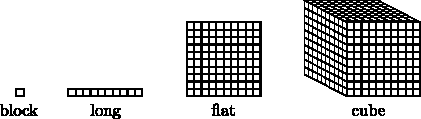
\includegraphics{../graphics/baseTenBlocks.pdf}
%\]

\fixnote{The division doesn't look good with slanted digits.  
Furthermore, the division might not be typesetting properly.  The tilde is intended to 
space by digitwidth, but this definition was commented out in the preamble because 
it caused the title control sequence to generate an error.}

\begin{problem}
Now Oscar is modeling the basic multiplication algorithm:
\[
\begin{tabular}{@{}r@{}}
11~~\\
234\\
$\times$~~3\\ \hline
702
\end{tabular}
\]
\begin{image}
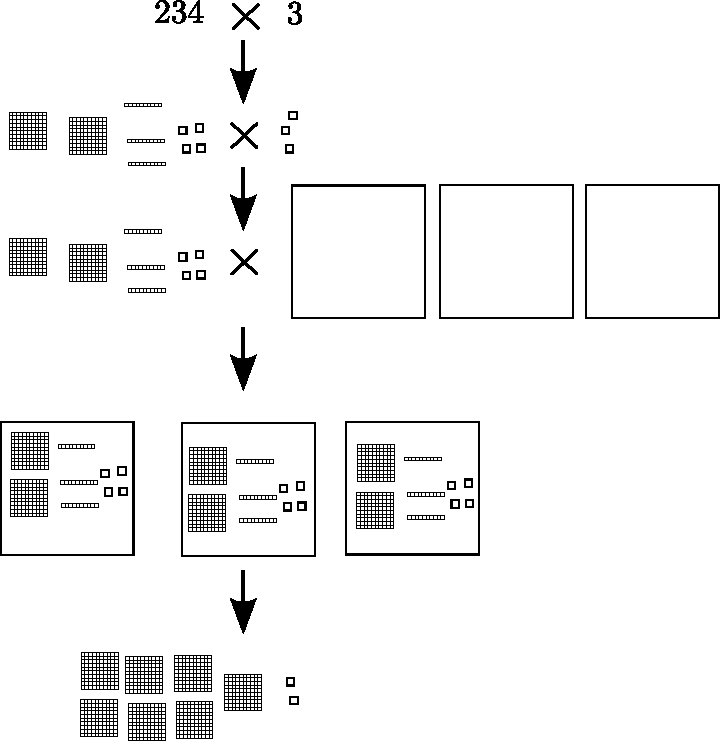
\includegraphics[scale=0.9]{oscarMult.pdf}
\end{image}
Can you explain what is going on?  Does his model illustrate the algorithm?  If so, explain how.  If not, describe how to use base ten blocks to explain the algorithm.  
\end{problem}

\begin{teachingnote}
This model doesn't show the separate steps in the algorithm.  It creates the three copies of 243 all at once rather than one place value at a time.  

The standard algorithm can be explained with blocks:  
\begin{itemize}
\item Three copies of four blocks makes 12 blocks.  Regroup as 1 long and 2 blocks. Write 2 below in blocks column and 1 above in longs column.
\item Three copies of three longs makes 9 longs.  Plus 1 long (from regrouping) makes 10 longs.  Regroup as 1 flat and 0 longs.  Write 0 below in the longs column and 1 above in the flats column.  
\item Three copies of 2 flats makes 6 flats.  Plus 1 flat (from regrouping) makes 7 flats.  Write 7 below in the flats column.  
\end{itemize}

And here is the ``behind the scenes algebra.''

\begin{align*}
234 \times 3 & = (2\cdot 10^2 + 3\cdot 10 + 4)\times 3 \\
&= 3\cdot 2\cdot 10^2 + 3\cdot 3\cdot 10 + 3\cdot 4 \\
&= 3\cdot 2\cdot 10^2 + 3\cdot 3\cdot 10 + 12 \\
&= 3\cdot 2\cdot 10^2 + 3\cdot 3\cdot 10 + 10 + 2\\
&= 3\cdot 2\cdot 10^2 + (3\cdot 3 + 1)\cdot 10 + 2\\
&= 3\cdot 2\cdot 10^2 + 10 \cdot 10 + 2\\
&= (3\cdot 2 + 1) \cdot 10^2 + 0 \cdot 10 + 2\\
&= 7\cdot 10^2 + 0 \cdot 10 + 2\\
&=702
\end{align*}
\end{teachingnote}

 
\begin{problem}
Here is an example of the basic division algorithm:
\[
3\,\begin{tabular}[b]{@{}r@{}r} 
67 &\, R$1$\\ 
\cline{1-1}
\Big)\begin{tabular}[t]{@{}l@{}} 202\\ 
18 \\ 
\divrule{0}{2}  ~22 \\
 ~21\\
 \divrule{1}{2}
~~1
\end{tabular}
\end{tabular}
\]
Explain how to model this algorithm with base-ten blocks, assuming that you start with 202 as two flats and two blocks and that you intend to organize them into three equal piles.  
\end{problem}

\begin{teachingnote}
\begin{itemize}
\item Encourage both 3 groups and groups of 3.  
\item For $202\div 3$, 3 doesn't go into 2 flats.  Regroup the 2 flats as 20 longs.  Then 3 groups gives 6 longs with for a total of 18 longs.  After subtraction, 2 longs are remaining. 
\item Regroup the 2 remaining longs as 20 blocks and combine with the 2 blocks to give 22 blocks.  
\item Organize the blocks into 3 groups give 7 blocks in each group for a total of 21 blocks.  After subtraction 1 block remains.  
\end{itemize}
\end{teachingnote}

\end{document}

%\documentclass[handout]{ximera}
\documentclass{ximera}

\usepackage{gensymb}
\usepackage{tabularx}
\usepackage{mdframed}
\usepackage{pdfpages}
%\usepackage{chngcntr}

\let\problem\relax
\let\endproblem\relax

\newcommand{\property}[2]{#1#2}




\newtheoremstyle{SlantTheorem}{\topsep}{\fill}%%% space between body and thm
 {\slshape}                      %%% Thm body font
 {}                              %%% Indent amount (empty = no indent)
 {\bfseries\sffamily}            %%% Thm head font
 {}                              %%% Punctuation after thm head
 {3ex}                           %%% Space after thm head
 {\thmname{#1}\thmnumber{ #2}\thmnote{ \bfseries(#3)}} %%% Thm head spec
\theoremstyle{SlantTheorem}
\newtheorem{problem}{Problem}[]

%\counterwithin*{problem}{section}



%%%%%%%%%%%%%%%%%%%%%%%%%%%%Jenny's code%%%%%%%%%%%%%%%%%%%%

%%% Solution environment
%\newenvironment{solution}{
%\ifhandout\setbox0\vbox\bgroup\else
%\begin{trivlist}\item[\hskip \labelsep\small\itshape\bfseries Solution\hspace{2ex}]
%\par\noindent\upshape\small
%\fi}
%{\ifhandout\egroup\else
%\end{trivlist}
%\fi}
%
%
%%% instructorIntro environment
%\ifhandout
%\newenvironment{instructorIntro}[1][false]%
%{%
%\def\givenatend{\boolean{#1}}\ifthenelse{\boolean{#1}}{\begin{trivlist}\item}{\setbox0\vbox\bgroup}{}
%}
%{%
%\ifthenelse{\givenatend}{\end{trivlist}}{\egroup}{}
%}
%\else
%\newenvironment{instructorIntro}[1][false]%
%{%
%  \ifthenelse{\boolean{#1}}{\begin{trivlist}\item[\hskip \labelsep\bfseries Instructor Notes:\hspace{2ex}]}
%{\begin{trivlist}\item[\hskip \labelsep\bfseries Instructor Notes:\hspace{2ex}]}
%{}
%}
%% %% line at the bottom} 
%{\end{trivlist}\par\addvspace{.5ex}\nobreak\noindent\hung} 
%\fi
%
%


\let\instructorNotes\relax
\let\endinstructorNotes\relax
%%% instructorNotes environment
\ifhandout
\newenvironment{instructorNotes}[1][false]%
{%
\def\givenatend{\boolean{#1}}\ifthenelse{\boolean{#1}}{\begin{trivlist}\item}{\setbox0\vbox\bgroup}{}
}
{%
\ifthenelse{\givenatend}{\end{trivlist}}{\egroup}{}
}
\else
\newenvironment{instructorNotes}[1][false]%
{%
  \ifthenelse{\boolean{#1}}{\begin{trivlist}\item[\hskip \labelsep\bfseries {\Large Instructor Notes: \\} \hspace{\textwidth} ]}
{\begin{trivlist}\item[\hskip \labelsep\bfseries {\Large Instructor Notes: \\} \hspace{\textwidth} ]}
{}
}
{\end{trivlist}}
\fi


%% Suggested Timing
\newcommand{\timing}[1]{{\bf Suggested Timing: \hspace{2ex}} #1}




\hypersetup{
    colorlinks=true,       % false: boxed links; true: colored links
    linkcolor=blue,          % color of internal links (change box color with linkbordercolor)
    citecolor=green,        % color of links to bibliography
    filecolor=magenta,      % color of file links
    urlcolor=cyan           % color of external links
}

\title{Comparative Arithmetic}
\author{Bart Snapp and Brad Findell}

\outcome{Learning outcome goes here.}

\begin{document}
\begin{abstract}
Abstract goes here.  
\end{abstract}
\maketitle

\label{A:CA}

\begin{teachingnote}
The point of the activity is that polynomial arithmetic is analogous to familiar base-ten algorithms, except there is no ``regrouping'' (i.e., carrying or borrowing).  Ultimately, we want students to see polynomials as numbers in base $x$ and to see base-ten numbers as polynomials in 10.
\end{teachingnote}

\begin{problem} Compute:
\[
\begin{array}{@{}r@{}}
131\\
+122\\ \hline
\end{array}
\qquad\text{and}
\qquad
\begin{array}{@{}r@{}}
x^2+3x+1\\
+x^2+2x+2\\ \hline
\end{array}
\]

\vspace{0.5in}
Compare, contrast, and describe your experiences.
\end{problem}

\begin{problem} Compute:
\[
\begin{array}{@{}r@{}}
139\\
+122\\ \hline
\end{array}
\qquad\text{and}
\qquad
\begin{array}{@{}r@{}}
x^2+3x+9\\
+x^2+2x+2\\ \hline
\end{array}
\]

\vspace{0.5in}
Compare, contrast, and describe your experiences. In particular,
discuss how this is different from the first problem.
\end{problem}


\begin{problem} Compute:
\[
\begin{array}{@{}r@{}}
121\\
\times 32\\ \hline
\end{array}
\qquad\text{and}
\qquad
\begin{array}{@{}r@{}}
x^2+2x+1\\
\times~~~3x+2\\ \hline
\end{array}
\]
\vspace{0.8in}

Compare, contrast, and describe your experiences.
\end{problem}

\begin{problem}
Expand:
\[
(x^2 + 2x + 1)(3x+2)
\]

\vspace{0.2in}
Compare, contrast, and describe your experiences. In particular, discuss how this problem relates to the one above.
\end{problem}

\begin{problem} Compute:
\[
\begin{array}{@{}r@{}}
214\\
\times 53\\ \hline
\end{array}
\qquad\text{and}
\qquad
\begin{array}{@{}r@{}}
2x^2+x+4\\
\times~~~5x+3\\ \hline
\end{array}
\]
Compare, contrast, and describe your experiences.
\end{problem}

\begin{problem}
Use long division to compute $2785\div 23$ and $(2x^3+7x^2+8x+5)\div (2x+3)$.  Compare, contrast, and describe your experiences.  
\end{problem}

\begin{problem}
Use long division to compute $6529\div 34$ and $(6x^3+5x^2+2x+9)\div (3x+4)$.  Compare, contrast, and describe your experiences.  
\end{problem}

\end{document}

\documentclass{ximera}

\usepackage{gensymb}
\usepackage{tabularx}
\usepackage{mdframed}
\usepackage{pdfpages}
%\usepackage{chngcntr}

\let\problem\relax
\let\endproblem\relax

\newcommand{\property}[2]{#1#2}




\newtheoremstyle{SlantTheorem}{\topsep}{\fill}%%% space between body and thm
 {\slshape}                      %%% Thm body font
 {}                              %%% Indent amount (empty = no indent)
 {\bfseries\sffamily}            %%% Thm head font
 {}                              %%% Punctuation after thm head
 {3ex}                           %%% Space after thm head
 {\thmname{#1}\thmnumber{ #2}\thmnote{ \bfseries(#3)}} %%% Thm head spec
\theoremstyle{SlantTheorem}
\newtheorem{problem}{Problem}[]

%\counterwithin*{problem}{section}



%%%%%%%%%%%%%%%%%%%%%%%%%%%%Jenny's code%%%%%%%%%%%%%%%%%%%%

%%% Solution environment
%\newenvironment{solution}{
%\ifhandout\setbox0\vbox\bgroup\else
%\begin{trivlist}\item[\hskip \labelsep\small\itshape\bfseries Solution\hspace{2ex}]
%\par\noindent\upshape\small
%\fi}
%{\ifhandout\egroup\else
%\end{trivlist}
%\fi}
%
%
%%% instructorIntro environment
%\ifhandout
%\newenvironment{instructorIntro}[1][false]%
%{%
%\def\givenatend{\boolean{#1}}\ifthenelse{\boolean{#1}}{\begin{trivlist}\item}{\setbox0\vbox\bgroup}{}
%}
%{%
%\ifthenelse{\givenatend}{\end{trivlist}}{\egroup}{}
%}
%\else
%\newenvironment{instructorIntro}[1][false]%
%{%
%  \ifthenelse{\boolean{#1}}{\begin{trivlist}\item[\hskip \labelsep\bfseries Instructor Notes:\hspace{2ex}]}
%{\begin{trivlist}\item[\hskip \labelsep\bfseries Instructor Notes:\hspace{2ex}]}
%{}
%}
%% %% line at the bottom} 
%{\end{trivlist}\par\addvspace{.5ex}\nobreak\noindent\hung} 
%\fi
%
%


\let\instructorNotes\relax
\let\endinstructorNotes\relax
%%% instructorNotes environment
\ifhandout
\newenvironment{instructorNotes}[1][false]%
{%
\def\givenatend{\boolean{#1}}\ifthenelse{\boolean{#1}}{\begin{trivlist}\item}{\setbox0\vbox\bgroup}{}
}
{%
\ifthenelse{\givenatend}{\end{trivlist}}{\egroup}{}
}
\else
\newenvironment{instructorNotes}[1][false]%
{%
  \ifthenelse{\boolean{#1}}{\begin{trivlist}\item[\hskip \labelsep\bfseries {\Large Instructor Notes: \\} \hspace{\textwidth} ]}
{\begin{trivlist}\item[\hskip \labelsep\bfseries {\Large Instructor Notes: \\} \hspace{\textwidth} ]}
{}
}
{\end{trivlist}}
\fi


%% Suggested Timing
\newcommand{\timing}[1]{{\bf Suggested Timing: \hspace{2ex}} #1}




\hypersetup{
    colorlinks=true,       % false: boxed links; true: colored links
    linkcolor=blue,          % color of internal links (change box color with linkbordercolor)
    citecolor=green,        % color of links to bibliography
    filecolor=magenta,      % color of file links
    urlcolor=cyan           % color of external links
}

\title{Addition with Integers}
\author{Vic Ferdinand, Betsy McNeal, Jenny Sheldon}

\begin{document}

\begin{abstract}
We look at adding integers.
\end{abstract}
\maketitle



Recall that when we think of addition as combining, we are taking two disjoint sets and joining them together into a new set.  The sum of the two sets' amounts is the amount in the newly formed set.  We also think of addition in a ``join add-to'' context, where we begin with one set and join a disjoint set to it.  Let's recall our most basic addition example.
\begin{example}
Johnny has $5$ apples, and Suzy has $3$ apples.  How many apples do Johnny and Suzy have all together?  Write an expression using the addition sign which solves this problem. $\answer[given]{5 + 3}$
\end{example}

If we change this example to a story about checks and bills, we might use the following instead.
\begin{example}
In yesterday's mail, Johnny received a check for \$$5$ and another check for \$$3$.  What is the total value of Johnny's checks and bills from yesterday?  Write an expression using the addition sign which solves this problem. $\answer[given]{5 + 3}$
\end{example}
Now we can easily extend our story to one involving negative numbers.
\begin{example}
In yesterday's mail, Johnny received a bill for \$$8$ and a check for \$$4$.  What is the total value of Johnny's checks and bills from yesterday?  Write an expression using the addition sign which solves this problem. $\answer[given]{-8 + 4}$
\end{example}
\begin{example}
In yesterday's mail, Johnny received a bill for \$$22$ and another bill for \$$54$.  What is the total value of Johnny's checks and bills from yesterday?  Write an expression using the addition sign which solves this problem. $\answer[given]{-22 + (-54)}$
\end{example}

There are several important things to notice with these examples.  First, our story gives us a good idea whether the overall answer of the story should be positive or negative.  In the case of two checks, we expect a positive number.  In the case of two bills, we expect a negative number.  In the case of a check and a bill, we would need to know the values of the objects.  This observation sets the stage for some important questions we want to consider about multiplying with negative numbers.  In particular, we would like to develop an intuition for why the product of two negative numbers is negative.  You might pause for a few minutes here to see if you already have some ideas about this concept.

Second, we need to exercise care with the question we ask in our checks and bills stories.  For instance, if we used the example of receiving two checks, one for \$$5$ and one for \$$3$, we could ask, ``What is our net worth now?''  In this case, we don't actually have enough information to answer the question.  If we began the day with a net worth of \$$84$, our new net worth would be \$$(84 + 5 + 3)$.  If instead we began the day in debt \$$9$, we are now in debt \$$1$.  We can modify this question to add the information that we began the day with no profit and no debt, but then our net worth would be \$$(0 + 5 + 3)$.  We now get the correct numerical value of \$$8$, since adding zero doesn't change our answer, but this is a different expression than \$$(5 + 3)$.  Be on the lookout for similar pitfalls as you write your own story problems.  You may find the ``join add-to'' model of addition easier to work with.
\begin{example}
Johnny has a net worth of \$$-4$, and then he receives a check for \$$14$.  What is Johnny's net worth now?  Write an expression using the addition sign which solves this problem.  $\answer[given]{-4+14}$.
\end{example}

Next, let's use a number line to solve some addition problems with integers.

\begin{question}
Imagine using a number line like the one below to solve the addition problem $5 + 3$.
\begin{center}
\begin{tikzpicture}[font=\Large]
\draw[<->] (-0.5,0) -- (12.5,0);
\foreach \x in {0,1.5, 3, 4.5, 6, 7.5, 9, 10.5,12}
\draw[shift={(\x,0)},color=black] (0pt,3pt) -- (0pt,-2pt);
\draw (0,0) node[below]{$-4$};
\draw (1.5,0) node[below]{$-3$};
\draw (3,0) node[below]{$-2$};
\draw (4.5,0) node[below]{$-1$};
\draw (6,0) node[below]{$0$};
\draw (7.5,0) node[below]{$1$};
\draw (9,0) node[below]{$2$};
\draw (10.5,0) node[below]{$3$};
\draw (12,0) node[below]{$4$};
\end{tikzpicture}  
\end{center}
We begin by standing on the number line at the tick marked with $\answer[given]{5}$.  Since we are adding, we face towards the \wordChoice{\choice[correct]{right} \choice{left}}.  We will move $\answer[given]{3}$ spaces \wordChoice{\choice[correct]{forward} \choice{backward}}, since $3$ is positive.  Where on the number line are we now? $\answer[given]{8}$
\end{question}

\begin{question}
Imagine using a number line like the one below to solve the addition problem $-8 + 4$.
\begin{center}
\begin{tikzpicture}[font=\Large]
\draw[<->] (-0.5,0) -- (12.5,0);
\foreach \x in {0,1.5, 3, 4.5, 6, 7.5, 9, 10.5,12}
\draw[shift={(\x,0)},color=black] (0pt,3pt) -- (0pt,-2pt);
\draw (0,0) node[below]{$-4$};
\draw (1.5,0) node[below]{$-3$};
\draw (3,0) node[below]{$-2$};
\draw (4.5,0) node[below]{$-1$};
\draw (6,0) node[below]{$0$};
\draw (7.5,0) node[below]{$1$};
\draw (9,0) node[below]{$2$};
\draw (10.5,0) node[below]{$3$};
\draw (12,0) node[below]{$4$};
\end{tikzpicture}  
\end{center}
We begin by standing on the number line at the tick marked with $\answer[given]{-8}$.  Since we are adding, we face towards the \wordChoice{\choice[correct]{right} \choice{left}}.  We will move $\answer[given]{4}$ spaces \wordChoice{\choice[correct]{forward} \choice{backward}}, since $4$ is positive.  Where on the number line are we now? $\answer[given]{-4}$
\end{question}

\begin{question}
Imagine using a number line like the one below to solve the addition problem $(-22) + (-54)$.
\begin{center}
\begin{tikzpicture}[font=\Large]
\draw[<->] (-0.5,0) -- (12.5,0);
\foreach \x in {0,1.5, 3, 4.5, 6, 7.5, 9, 10.5,12}
\draw[shift={(\x,0)},color=black] (0pt,3pt) -- (0pt,-2pt);
\draw (0,0) node[below]{$-4$};
\draw (1.5,0) node[below]{$-3$};
\draw (3,0) node[below]{$-2$};
\draw (4.5,0) node[below]{$-1$};
\draw (6,0) node[below]{$0$};
\draw (7.5,0) node[below]{$1$};
\draw (9,0) node[below]{$2$};
\draw (10.5,0) node[below]{$3$};
\draw (12,0) node[below]{$4$};
\end{tikzpicture}  
\end{center}
We begin by standing on the number line at the tick marked with $\answer[given]{-22}$.  Since we are adding, we face towards the \wordChoice{\choice[correct]{right} \choice{left}}.  We will move $\answer[given]{54}$ spaces \wordChoice{\choice{forward} \choice[correct]{backward}}, since $54$ is negative.  Where on the number line are we now? $\answer[given]{-76}$
\end{question}

Again, notice that our movement on the number line gives us a sense as to whether the final answer should be positive or negative!

Finally, we investigate addition of negative numbers via patterns.
\begin{example}
Consider the sequence of addition problems.
\begin{align*}
5 + 4 &= \answer[given]{9} \\
5 + 3 &= \answer[given]{8} \\
5 + 2 &= \answer[given]{7} \\
5 + 1 &= \answer[given]{6} \\
5 + 0 &= \answer[given]{5}
\end{align*}
As we move down the chart, moving one row down results in the final answer decreasing by $\answer[given]{1}$.  So, if the pattern continues to hold, we expect the answer to $5 + (-1)$ to be $\answer[given]{4}$, since it is one less than $5$.
\end{example}
Try your hand at recognizing patterns with some other addition problems.

Finally, notice that no matter how we approach the problems in this section, we are getting consistent answers.  Whether we use a combining or join add-to addition structure, we get the same answer.  Whether we use a checks and bills story, a number line, or a pattern, we are always getting the same answer.  This is not only comforting, it is necessary for addition as an operation!

\end{document}
%\documentclass[handout]{ximera}
\documentclass{ximera}

\usepackage{gensymb}
\usepackage{tabularx}
\usepackage{mdframed}
\usepackage{pdfpages}
%\usepackage{chngcntr}

\let\problem\relax
\let\endproblem\relax

\newcommand{\property}[2]{#1#2}




\newtheoremstyle{SlantTheorem}{\topsep}{\fill}%%% space between body and thm
 {\slshape}                      %%% Thm body font
 {}                              %%% Indent amount (empty = no indent)
 {\bfseries\sffamily}            %%% Thm head font
 {}                              %%% Punctuation after thm head
 {3ex}                           %%% Space after thm head
 {\thmname{#1}\thmnumber{ #2}\thmnote{ \bfseries(#3)}} %%% Thm head spec
\theoremstyle{SlantTheorem}
\newtheorem{problem}{Problem}[]

%\counterwithin*{problem}{section}



%%%%%%%%%%%%%%%%%%%%%%%%%%%%Jenny's code%%%%%%%%%%%%%%%%%%%%

%%% Solution environment
%\newenvironment{solution}{
%\ifhandout\setbox0\vbox\bgroup\else
%\begin{trivlist}\item[\hskip \labelsep\small\itshape\bfseries Solution\hspace{2ex}]
%\par\noindent\upshape\small
%\fi}
%{\ifhandout\egroup\else
%\end{trivlist}
%\fi}
%
%
%%% instructorIntro environment
%\ifhandout
%\newenvironment{instructorIntro}[1][false]%
%{%
%\def\givenatend{\boolean{#1}}\ifthenelse{\boolean{#1}}{\begin{trivlist}\item}{\setbox0\vbox\bgroup}{}
%}
%{%
%\ifthenelse{\givenatend}{\end{trivlist}}{\egroup}{}
%}
%\else
%\newenvironment{instructorIntro}[1][false]%
%{%
%  \ifthenelse{\boolean{#1}}{\begin{trivlist}\item[\hskip \labelsep\bfseries Instructor Notes:\hspace{2ex}]}
%{\begin{trivlist}\item[\hskip \labelsep\bfseries Instructor Notes:\hspace{2ex}]}
%{}
%}
%% %% line at the bottom} 
%{\end{trivlist}\par\addvspace{.5ex}\nobreak\noindent\hung} 
%\fi
%
%


\let\instructorNotes\relax
\let\endinstructorNotes\relax
%%% instructorNotes environment
\ifhandout
\newenvironment{instructorNotes}[1][false]%
{%
\def\givenatend{\boolean{#1}}\ifthenelse{\boolean{#1}}{\begin{trivlist}\item}{\setbox0\vbox\bgroup}{}
}
{%
\ifthenelse{\givenatend}{\end{trivlist}}{\egroup}{}
}
\else
\newenvironment{instructorNotes}[1][false]%
{%
  \ifthenelse{\boolean{#1}}{\begin{trivlist}\item[\hskip \labelsep\bfseries {\Large Instructor Notes: \\} \hspace{\textwidth} ]}
{\begin{trivlist}\item[\hskip \labelsep\bfseries {\Large Instructor Notes: \\} \hspace{\textwidth} ]}
{}
}
{\end{trivlist}}
\fi


%% Suggested Timing
\newcommand{\timing}[1]{{\bf Suggested Timing: \hspace{2ex}} #1}




\hypersetup{
    colorlinks=true,       % false: boxed links; true: colored links
    linkcolor=blue,          % color of internal links (change box color with linkbordercolor)
    citecolor=green,        % color of links to bibliography
    filecolor=magenta,      % color of file links
    urlcolor=cyan           % color of external links
}

\title{Integer Multiplication}
\author{Bart Snapp and Brad Findell}

\outcome{Learning outcome goes here.}

\begin{document}
\begin{abstract}
Abstract goes here.  
\end{abstract}
\maketitle

\label{A:integerMultiplication}

In this activity, we explore various models and strategies for 
making sense of multiplication of integers.  

\subsection*{Continuing patterns}
\begin{problem}
\begin{enumerate}
\item Continue the following patterns, and explain why it makes sense to continue them in that way.    

\fixnote{Table doesn't look great.}

\begin{minipage}{0.45\textwidth}
\begin{align*}
4\times 3 &= 12 \\
4\times 2 &= \\
4\times 1 &= \\
4\times 0 &= \\
4\times (-1) &= \\
4\times (-2) &= \\
4\times (-3) &= \\
\end{align*}
\end{minipage}
\begin{minipage}{0.45\textwidth}
\begin{align*}
3\times 6 &= 18 \\
2\times 6 &= \\
1\times 6 &= \\
0\times 6 &= \\
(-1)\times 6 &= \\
(-2)\times 6 &= \\
(-3)\times 6 &= \\
\end{align*}
\end{minipage}
\begin{minipage}{0.45\textwidth}
\begin{align*}
(-7)\times 3 &= -21 \\
(-7)\times 2 &= \\
(-7)\times 1 &= \\
(-7)\times 0 &= \\
(-7)\times (-1) &= \\
(-7)\times (-2) &= \\
(-7)\times (-3) &= \\
\end{align*}
\end{minipage}

\item What rule of multiplication might a student infer from the first pattern? 
\item What rule of multiplication might a student infer from the second pattern?
\item What rule of multiplication might a student infer from the third pattern?
\end{enumerate}
\begin{teachingnote}
As a shorthand, consider each pattern of the form $ab = c$.  We want students to describe the following:  
\begin{itemize}
\item First pattern:  For $4\cdot b = c$, decreasing $b$ by one results in a decrease of $c$ by 4.  Then notice that $4(-b) = -4b$, which illustrates that a positive times a negative should be negative. 
\item Second pattern:  For $a\cdot 6= c$, decreasing $a$ by one results in a decrease of $c$ by 6.  Then notice that $(-a)6 = -(a\cdot 6)$, which illustrates that a negative times a positive should be negative.  
\item Third pattern:  For $(-7)\cdot b= c$, decreasing $b$ by one results in a increase of $c$ by 7.  Then notice that $-7\cdot (-b) = 7b $, which illustrates that a negative times a negative should be positive. 
\end{itemize}
These illustrations are not proofs, but they reveal that the distributive property is in play.  
\end{teachingnote}
\end{problem}

\subsection*{Using properties of operations}

\begin{problem}
Suppose we \emph{do not know} how to multiply negative numbers but we do know that $4\times 6=24$. We will use this fact and the properties of operations to reason about products involving negative numbers.  
\begin{enumerate}
\item What do we know about $A$ and $B$ if $A+B=0$?  
\item Use the distributive property to show that the expression $4\times 6 + 4\times(-6)$ is equal to $0$.  
Then use that fact to reason about what $4\times(-6)$ should be.  
\item Use the distributive property to show that the expression $4\times (-6) + (-4)\times (-6)$ is equal to $0$.  
Then use that fact to reason about what $(-4)\times(-6)$ should be.  
\end{enumerate}
\end{problem}

\subsection*{Walking on a number line}
\begin{teachingnote}
Again there are two decisions to make: (1) distinguishing positive and negative for the multiplicand; (2) distinguishing positive and negative for the multiplier.
\end{teachingnote}
\begin{problem} 
Matt is a member of the Ohio State University
  Marching Band. Being rather capable, Matt can take $x$ steps of size
  $y$ inches for all integer values of $x$ and $y$.  If $x$ is
  positive it means \textit{face North and take $x$ steps.} If $x$ is
  negative it means \textit{face South and take $|x|$ steps.} If $y$
  is positive it means your step is a \textit{forward step of $y$
    inches.} If $y$ is negative it means your step \textit{is a
    backward step of $|y|$ inches.}
\begin{enumerate}
\item Discuss what the expressions $x \cdot y$ means in this
  context. In particular, what happens if $x = 1$? What if $y=1$?
\item If $x$ and $y$ are both positive, how does this fit with the ``repeated addition'' model of multiplication?    
\item Using the context above and specific numbers, 
demonstrate the general rule:
\[
\text{negative}\cdot \text{positive} = \text{negative}
\]
Clearly explain how your problem shows this.
\item Using the context above and specific numbers, 
demonstrate the general rule:
\[
\text{positive}\cdot \text{negative} = \text{negative}
\]
Clearly explain how your problem shows this.\item Using the context above and specific numbers, 
demonstrate the general rule:
\[
\text{negative}\cdot \text{negative} = \text{positive}
\]
Clearly explain how your problem shows this.
\end{enumerate}
\end{problem}

\end{document}
\newpage
\section{What Can Division Mean?}\label{A:dm}
\begin{teachingnote}
Two models of division:  
\begin{itemize}
\item ``How many in one group?'' questions use the ``sharing'' model of division.  
\item ``How many groups?'' questions use what is sometimes called the ``measurement'' model of division.  
\end{itemize}
Division problems can have many types of answers, depending on the numbers and the context:
\begin{enumerate}
\item exact division (i.e., no remainder)
\item complete division (e.g., with a fractional part)
\item quotient and remainder (i.e., two numbers with different meanings)
\item just the quotient (i.e.,ignoring a non-zero remainder, rounding down)
\item quotient rounded up 
\item just the remainder
\end{enumerate}
\end{teachingnote}
Solve each of the problems below, explain your reasoning, and indicate whether the problem is asking ``\textbf{How many in one group?}'' or ``\textbf{How many groups?}'' or something else entirely.

\begin{prob}
There are a total of $35$ hard candies. If there are $5$ boxes with an
equal number of candies in each box---and all the candy is accounted
for, then how many candies are in each box? What if you had $39$
candies?
\end{prob}

\begin{prob}
There are a total of $28$ hard candies. If there are $4$ candies in
each box, how many boxes are there? What if you had $34$ candies?
\end{prob}


\begin{prob}
There is a total of 29 gallons of milk to be put in 6 containers.  If
each container holds the same amount of milk and all the milk is
accounted for, how much milk will each container hold?
\end{prob}

 
\begin{prob}
There is a total of 29 gallons of milk to be sold in containers holding
6 gallons each.  If all the milk is used, how many containers can be sold?
\end{prob}

\begin{prob}
There is a total of 29 gallons of milk to be sold in containers holding
6 gallons each.  If all the milk is used, how much milk cannot be sold?
\end{prob}
 
\begin{prob}
If there are 29 kids and each van holds 6 kids, how many vans do
we need for the field trip?
\end{prob}


%\begin{prob}
%Paolo has a total of $48$ outfits (shirts and pants) he can wear. If
%he has $8$ shirts, how many pants does he have?
%\end{prob}

%\begin{prob}
%A chart has $72$ cells and $8$ rows. How many columns does it have?
%\end{prob}

%\begin{prob} 
%A rectangle has a length of $6$ inches and an area of $42$ square
%inches. What is its width?
%\end{prob}

%\begin{prob} 
%Can you think of a division problem that is fundamentally different
%from the problems above?
%\end{prob}

%\begin{prob} 
%In the context of the problems above, what might ``division by zero''
%mean?
%\end{prob}



%\documentclass[handout]{ximera}
\documentclass{ximera}

\usepackage{gensymb}
\usepackage{tabularx}
\usepackage{mdframed}
\usepackage{pdfpages}
%\usepackage{chngcntr}

\let\problem\relax
\let\endproblem\relax

\newcommand{\property}[2]{#1#2}




\newtheoremstyle{SlantTheorem}{\topsep}{\fill}%%% space between body and thm
 {\slshape}                      %%% Thm body font
 {}                              %%% Indent amount (empty = no indent)
 {\bfseries\sffamily}            %%% Thm head font
 {}                              %%% Punctuation after thm head
 {3ex}                           %%% Space after thm head
 {\thmname{#1}\thmnumber{ #2}\thmnote{ \bfseries(#3)}} %%% Thm head spec
\theoremstyle{SlantTheorem}
\newtheorem{problem}{Problem}[]

%\counterwithin*{problem}{section}



%%%%%%%%%%%%%%%%%%%%%%%%%%%%Jenny's code%%%%%%%%%%%%%%%%%%%%

%%% Solution environment
%\newenvironment{solution}{
%\ifhandout\setbox0\vbox\bgroup\else
%\begin{trivlist}\item[\hskip \labelsep\small\itshape\bfseries Solution\hspace{2ex}]
%\par\noindent\upshape\small
%\fi}
%{\ifhandout\egroup\else
%\end{trivlist}
%\fi}
%
%
%%% instructorIntro environment
%\ifhandout
%\newenvironment{instructorIntro}[1][false]%
%{%
%\def\givenatend{\boolean{#1}}\ifthenelse{\boolean{#1}}{\begin{trivlist}\item}{\setbox0\vbox\bgroup}{}
%}
%{%
%\ifthenelse{\givenatend}{\end{trivlist}}{\egroup}{}
%}
%\else
%\newenvironment{instructorIntro}[1][false]%
%{%
%  \ifthenelse{\boolean{#1}}{\begin{trivlist}\item[\hskip \labelsep\bfseries Instructor Notes:\hspace{2ex}]}
%{\begin{trivlist}\item[\hskip \labelsep\bfseries Instructor Notes:\hspace{2ex}]}
%{}
%}
%% %% line at the bottom} 
%{\end{trivlist}\par\addvspace{.5ex}\nobreak\noindent\hung} 
%\fi
%
%


\let\instructorNotes\relax
\let\endinstructorNotes\relax
%%% instructorNotes environment
\ifhandout
\newenvironment{instructorNotes}[1][false]%
{%
\def\givenatend{\boolean{#1}}\ifthenelse{\boolean{#1}}{\begin{trivlist}\item}{\setbox0\vbox\bgroup}{}
}
{%
\ifthenelse{\givenatend}{\end{trivlist}}{\egroup}{}
}
\else
\newenvironment{instructorNotes}[1][false]%
{%
  \ifthenelse{\boolean{#1}}{\begin{trivlist}\item[\hskip \labelsep\bfseries {\Large Instructor Notes: \\} \hspace{\textwidth} ]}
{\begin{trivlist}\item[\hskip \labelsep\bfseries {\Large Instructor Notes: \\} \hspace{\textwidth} ]}
{}
}
{\end{trivlist}}
\fi


%% Suggested Timing
\newcommand{\timing}[1]{{\bf Suggested Timing: \hspace{2ex}} #1}




\hypersetup{
    colorlinks=true,       % false: boxed links; true: colored links
    linkcolor=blue,          % color of internal links (change box color with linkbordercolor)
    citecolor=green,        % color of links to bibliography
    filecolor=magenta,      % color of file links
    urlcolor=cyan           % color of external links
}

\title{Divisibility Statements}
\author{Bart Snapp and Brad Findell}

\outcome{Learning outcome goes here.}

\begin{document}
\begin{abstract}
Abstract goes here.  
\end{abstract}
\maketitle

\label{A:divisibilityStatements}

Let $a|b$ mean $b=aq$ for some integer $q$.  (Read $a|b$ as ``$a$ divides $b$''.)  

\begin{problem}
Using the numbers 56 and 7, make some true statements using the notation above and one or more of the words factor, multiple, divisor, and divides.  
\end{problem}

\begin{problem}
Use the definition of \emph{divides} to decide which of the following are true and which are false.  If a statement is true, find $q$ satisfying the definition of divides.  If it is false, give an explanation.  (Hint:  Try to reason about multiplication without actually multiplying.)
\begin{enumerate}
\item $21|2121$
\item $3|(9\times 41)$
\item $6|(2^4\times 3^2\times 7^3\times 13^5)$
\item $100000|(2^3\times 3^9\times 5^{11}\times 17^8)$
\item $6000|(2^{21}\times 3^7 \times 5^{17}\times 29^5)$
\item $p^3q^5r|(p^5q^{13}r^7s^2t^{27})$
\item $7|(5\times 21 + 14)$
\end{enumerate}
\end{problem}

\begin{teachingnote}
Some students will write $2^4\cdot 3^2=6^6$.  Some students will insist on multiplying and dividing with their calculators. 

The following problems are challenging but worth the time.
\end{teachingnote}

\begin{problem}
If $a|b$ does $a|(bc)$?  Explain. 
\end{problem}

\begin{problem}
If $a|(bc)$ does $a|b$?  Explain. 
\end{problem}

\begin{problem}
If $a|b$ and $a|c$ does $a|(b+c)$?  Explain.  
\end{problem}

\begin{problem}
If $a|(b+c)$ does $a|b$ and $a|c$?  Explain.  
\end{problem}

\begin{problem}
If $a|(b+c)$ and $a|c$ does $a|b$?  Explain.  
\end{problem}

\begin{problem}
Suppose that $$(3^5\cdot 7^9\cdot 11^x\cdot 13^y)|(3^a\cdot 7^b\cdot 11^{19}\cdot 13^7)$$
What values of $a$, $b$, $x$, and $y$ make true statements? 
\end{problem}

\end{document}

\newpage
\section{Hall of Shoes}\label{A:Hall}
  
\begin{prob}  
\textit{Incognito's Hall of Shoes} is a shoe store that just
  opened in Myrtle Beach, South Carolina. At the moment, they have 100
  pairs of shoes in stock. At their grand opening 100 customers showed
  up. The first customer tried on every pair of shoes, the second
  customer tried on every 2nd pair, the third customer tried on every
  3rd pair, and so on until the 100th customer, who only tried on the
  last pair of shoes.
\begin{enumerate}
\item Which shoes were tried on by only 1 customer?
\item Which shoes were tried on by exactly 2 customers?
\item Which shoes were tried on by exactly 3 customers?
\item Which shoes were tried on by exactly 4 customers?
\item How many customers tried on the 45th pair?  
\item How many customers tried on the 81st pair?  
\item Challenge:  Which shoes were tried on by the most customers?  
\end{enumerate}
In each case, explain your reasoning.
\end{prob}

\begin{prob}
Which pairs of shoes were tried on by both 
\begin{enumerate}
\item customers 3 and 5?
\item customers 6 and 8?
\item customers 12 and 30?
\item customers 7 and 13?
\item customers $a$ and $b$?  
\end{enumerate}
\end{prob}

\begin{prob}
Which customers tried on both 
\begin{enumerate}
\item pairs 24 and 36?
\item pairs 30 and 60?
\item pairs 42 and 12?
\item pairs 28 and 15?
\item pairs $a$ and $b$?  
\end{enumerate}
\end{prob}



\newpage
\section{Sieving It All Out}\label{A:Sieve}

\begin{prob} 
Try to find all the primes from $1$ to $120$ \textit{without}
doing any division.  Try to circle numbers that are prime and 
cross out numbers that are not prime.  
As a gesture of friendship, here are the numbers from $1$ to $120$.
\[
\begin{tabular}{r r r r r r r r r r}

  1 &   2 &   3 &   4 &   5 &   6 &   7 &   8 &   9 &  10\\
  \\
 11 &  12 &  13 &  14 &  15 &  16 &  17 &  18 &  19 &  20\\
 \\
 21 &  22 &  23 &  24 &  25 &  26 &  27 &  28 &  29 &  30\\
 \\
 31 &  32 &  33 &  34 &  35 &  36 &  37 &  38 &  39 &  40\\
 \\
 41 &  42 &  43 &  44 &  45 &  46 &  47 &  48 &  49 &  50\\
 \\
 51 &  52 &  53 &  54 &  55 &  56 &  57 &  58 &  59 &  60\\
 \\
 61 &  62 &  63 &  64 &  65 &  66 &  67 &  68 &  69 &  70\\
 \\
 71 &  72 &  73 &  74 &  75 &  76 &  77 &  78 &  79 &  80\\
 \\
 81 &  82 &  83 &  84 &  85 &  86 &  87 &  88 &  89 &  90\\
 \\
 91 &  92 &  93 &  94 &  95 &  96 &  97 &  98 &  99 & 100\\
 \\
101 & 102 & 103 & 104 & 105 & 106 & 107 & 108 & 109 & 110\\
\\
111 & 112 & 113 & 114 & 115 & 116 & 117 & 118 & 119 & 120\\
\end{tabular}
\]

Describe your method.  
\end{prob}

\newpage

\begin{prob}
Now let's be systematic.  Ignore 1 (we'll talk about why later).   
As you identify a prime, first circle it, then cross out its multiples that are not already crossed out.  
Keep track of your work so that you can answer the following questions:  
\begin{enumerate}
\item After circling a new prime, note the first number crossed out with that prime.  Record your results in a table.
\marginfigure{%\footnotesize\sffamily
{\renewcommand{\arraystretch}{1.4}
\begin{tabular}{c|c}
        prime    & first \# crossed out \\
%                     & crossed out   \\
\hline
         2       &                      \\
                 &                      \\
                 &                      \\
                 &                      \\
                 &                      \\
\end{tabular}
}}
\item What was the biggest prime for which you crossed out at least one multiple?
\end{enumerate}

\begin{teachingnote}
When being systematic, the first number crossed out should be the square of the circled prime.  (All earlier multiples should have been crossed out because of smaller primes.)  

A quick check for the carefulness of the process is to look at $119 = 7 \times 17$. 

Side note:  When the sieve is done in six columns, we can observe that any prime greater than 3 must be one more or one less than a multiple of 6.
\end{teachingnote}

\[
\begin{tabular}{r r r r r r r r r r}

  1 &   2 &   3 &   4 &   5 &   6 &   7 &   8 &   9 &  10\\
  \\
 11 &  12 &  13 &  14 &  15 &  16 &  17 &  18 &  19 &  20\\
 \\
 21 &  22 &  23 &  24 &  25 &  26 &  27 &  28 &  29 &  30\\
 \\
 31 &  32 &  33 &  34 &  35 &  36 &  37 &  38 &  39 &  40\\
 \\
 41 &  42 &  43 &  44 &  45 &  46 &  47 &  48 &  49 &  50\\
 \\
 51 &  52 &  53 &  54 &  55 &  56 &  57 &  58 &  59 &  60\\
 \\
 61 &  62 &  63 &  64 &  65 &  66 &  67 &  68 &  69 &  70\\
 \\
 71 &  72 &  73 &  74 &  75 &  76 &  77 &  78 &  79 &  80\\
 \\
 81 &  82 &  83 &  84 &  85 &  86 &  87 &  88 &  89 &  90\\
 \\
 91 &  92 &  93 &  94 &  95 &  96 &  97 &  98 &  99 & 100\\
 \\
101 & 102 & 103 & 104 & 105 & 106 & 107 & 108 & 109 & 110\\
\\
111 & 112 & 113 & 114 & 115 & 116 & 117 & 118 & 119 & 120\\
\end{tabular}
\]
\end{prob}


%\begin{prob}
%Find all of the prime factors of 1008. How can you be sure you've
%found them all?
%\end{prob}

%\documentclass[handout]{ximera}
\documentclass[nooutcomes]{ximera}

\usepackage{gensymb}
\usepackage{tabularx}
\usepackage{mdframed}
\usepackage{pdfpages}
%\usepackage{chngcntr}

\let\problem\relax
\let\endproblem\relax

\newcommand{\property}[2]{#1#2}




\newtheoremstyle{SlantTheorem}{\topsep}{\fill}%%% space between body and thm
 {\slshape}                      %%% Thm body font
 {}                              %%% Indent amount (empty = no indent)
 {\bfseries\sffamily}            %%% Thm head font
 {}                              %%% Punctuation after thm head
 {3ex}                           %%% Space after thm head
 {\thmname{#1}\thmnumber{ #2}\thmnote{ \bfseries(#3)}} %%% Thm head spec
\theoremstyle{SlantTheorem}
\newtheorem{problem}{Problem}[]

%\counterwithin*{problem}{section}



%%%%%%%%%%%%%%%%%%%%%%%%%%%%Jenny's code%%%%%%%%%%%%%%%%%%%%

%%% Solution environment
%\newenvironment{solution}{
%\ifhandout\setbox0\vbox\bgroup\else
%\begin{trivlist}\item[\hskip \labelsep\small\itshape\bfseries Solution\hspace{2ex}]
%\par\noindent\upshape\small
%\fi}
%{\ifhandout\egroup\else
%\end{trivlist}
%\fi}
%
%
%%% instructorIntro environment
%\ifhandout
%\newenvironment{instructorIntro}[1][false]%
%{%
%\def\givenatend{\boolean{#1}}\ifthenelse{\boolean{#1}}{\begin{trivlist}\item}{\setbox0\vbox\bgroup}{}
%}
%{%
%\ifthenelse{\givenatend}{\end{trivlist}}{\egroup}{}
%}
%\else
%\newenvironment{instructorIntro}[1][false]%
%{%
%  \ifthenelse{\boolean{#1}}{\begin{trivlist}\item[\hskip \labelsep\bfseries Instructor Notes:\hspace{2ex}]}
%{\begin{trivlist}\item[\hskip \labelsep\bfseries Instructor Notes:\hspace{2ex}]}
%{}
%}
%% %% line at the bottom} 
%{\end{trivlist}\par\addvspace{.5ex}\nobreak\noindent\hung} 
%\fi
%
%


\let\instructorNotes\relax
\let\endinstructorNotes\relax
%%% instructorNotes environment
\ifhandout
\newenvironment{instructorNotes}[1][false]%
{%
\def\givenatend{\boolean{#1}}\ifthenelse{\boolean{#1}}{\begin{trivlist}\item}{\setbox0\vbox\bgroup}{}
}
{%
\ifthenelse{\givenatend}{\end{trivlist}}{\egroup}{}
}
\else
\newenvironment{instructorNotes}[1][false]%
{%
  \ifthenelse{\boolean{#1}}{\begin{trivlist}\item[\hskip \labelsep\bfseries {\Large Instructor Notes: \\} \hspace{\textwidth} ]}
{\begin{trivlist}\item[\hskip \labelsep\bfseries {\Large Instructor Notes: \\} \hspace{\textwidth} ]}
{}
}
{\end{trivlist}}
\fi


%% Suggested Timing
\newcommand{\timing}[1]{{\bf Suggested Timing: \hspace{2ex}} #1}




\hypersetup{
    colorlinks=true,       % false: boxed links; true: colored links
    linkcolor=blue,          % color of internal links (change box color with linkbordercolor)
    citecolor=green,        % color of links to bibliography
    filecolor=magenta,      % color of file links
    urlcolor=cyan           % color of external links
}

\title{There's Always Another Prime}
\author{Bart Snapp and Brad Findell}

\outcome{Learning outcome goes here.}

\begin{document}
\begin{abstract}
  We think about the number of prime numbers.
\end{abstract}
\maketitle

\label{A:Pr}

We'll start off with easy questions, then move to harder ones.  

\begin{problem}
Use the Division Theorem to explain why neither $2$ nor $3$ divides
$2\cdot 3+1$.  (Hint:  Do not multiply and add.  Use the expression 
as written to reason what the quotient and remainder must be.)
\end{problem}

\begin{problem}
Use the Division Theorem to explain why neither $2$ nor $3$ nor $5$ divides
$2\cdot 3\cdot 5+1$.
\end{problem}

\begin{problem} 
Let $p_1,\dots, p_n$ be the first $n$ primes. Do any of these primes divide 
\[
p_1p_2\cdots p_n + 1?
\]
Explain your reasoning.
\end{problem}


\begin{problem} 
Suppose there were only a finite number of primes, say there were only
$n$ of them. Call them $p_1,\dots, p_n$. Could any of them divide
\[
p_1p_2\cdots p_n + 1?
\]
what does that mean? Can there really only be a finite number of
primes?
\end{problem}


\begin{problem} 
Consider the following:
\[
2\cdot 3\cdot 5\cdot 7 \cdot 11\cdot 13 + 1 = 59\cdot 509
\] 
Does this contradict our work above? If so, explain why. If not, explain
why not.
\end{problem}

\end{document}

%\documentclass[handout]{ximera}
\documentclass[nooutcomes]{ximera}

\usepackage{gensymb}
\usepackage{tabularx}
\usepackage{mdframed}
\usepackage{pdfpages}
%\usepackage{chngcntr}

\let\problem\relax
\let\endproblem\relax

\newcommand{\property}[2]{#1#2}




\newtheoremstyle{SlantTheorem}{\topsep}{\fill}%%% space between body and thm
 {\slshape}                      %%% Thm body font
 {}                              %%% Indent amount (empty = no indent)
 {\bfseries\sffamily}            %%% Thm head font
 {}                              %%% Punctuation after thm head
 {3ex}                           %%% Space after thm head
 {\thmname{#1}\thmnumber{ #2}\thmnote{ \bfseries(#3)}} %%% Thm head spec
\theoremstyle{SlantTheorem}
\newtheorem{problem}{Problem}[]

%\counterwithin*{problem}{section}



%%%%%%%%%%%%%%%%%%%%%%%%%%%%Jenny's code%%%%%%%%%%%%%%%%%%%%

%%% Solution environment
%\newenvironment{solution}{
%\ifhandout\setbox0\vbox\bgroup\else
%\begin{trivlist}\item[\hskip \labelsep\small\itshape\bfseries Solution\hspace{2ex}]
%\par\noindent\upshape\small
%\fi}
%{\ifhandout\egroup\else
%\end{trivlist}
%\fi}
%
%
%%% instructorIntro environment
%\ifhandout
%\newenvironment{instructorIntro}[1][false]%
%{%
%\def\givenatend{\boolean{#1}}\ifthenelse{\boolean{#1}}{\begin{trivlist}\item}{\setbox0\vbox\bgroup}{}
%}
%{%
%\ifthenelse{\givenatend}{\end{trivlist}}{\egroup}{}
%}
%\else
%\newenvironment{instructorIntro}[1][false]%
%{%
%  \ifthenelse{\boolean{#1}}{\begin{trivlist}\item[\hskip \labelsep\bfseries Instructor Notes:\hspace{2ex}]}
%{\begin{trivlist}\item[\hskip \labelsep\bfseries Instructor Notes:\hspace{2ex}]}
%{}
%}
%% %% line at the bottom} 
%{\end{trivlist}\par\addvspace{.5ex}\nobreak\noindent\hung} 
%\fi
%
%


\let\instructorNotes\relax
\let\endinstructorNotes\relax
%%% instructorNotes environment
\ifhandout
\newenvironment{instructorNotes}[1][false]%
{%
\def\givenatend{\boolean{#1}}\ifthenelse{\boolean{#1}}{\begin{trivlist}\item}{\setbox0\vbox\bgroup}{}
}
{%
\ifthenelse{\givenatend}{\end{trivlist}}{\egroup}{}
}
\else
\newenvironment{instructorNotes}[1][false]%
{%
  \ifthenelse{\boolean{#1}}{\begin{trivlist}\item[\hskip \labelsep\bfseries {\Large Instructor Notes: \\} \hspace{\textwidth} ]}
{\begin{trivlist}\item[\hskip \labelsep\bfseries {\Large Instructor Notes: \\} \hspace{\textwidth} ]}
{}
}
{\end{trivlist}}
\fi


%% Suggested Timing
\newcommand{\timing}[1]{{\bf Suggested Timing: \hspace{2ex}} #1}




\hypersetup{
    colorlinks=true,       % false: boxed links; true: colored links
    linkcolor=blue,          % color of internal links (change box color with linkbordercolor)
    citecolor=green,        % color of links to bibliography
    filecolor=magenta,      % color of file links
    urlcolor=cyan           % color of external links
}

\title{There Are Many Factors to Consider}
\author{Bart Snapp and Brad Findell}

\outcome{Learning outcome goes here.}

\begin{document}
\begin{abstract}
  We count the number of factors of an integer.
\end{abstract}
\maketitle

\label{A:CF}

Suppose we want to know how many factors $43,\!560$ has, but we don't need to list them all.  In this activity we develop a method for computing the number of factors of a number.  

\begin{teachingnote}
Maybe begin by asking student to list all the factors of $43,\!560$, in hopes that they will feel compelled to find a more efficient strategy.
\end{teachingnote}

\begin{problem}
Vic listed the following factors of 80:  1, 2, 4, 5, 8, 10, 20, 40, 80.  What is missing? Describe your method of checking the list.  
\vspace{0.2in}
\begin{teachingnote}
We hope they are organizing the factors in pairs and that they notice the $5$ has no ``partner.''  
\end{teachingnote}
\end{problem}

\begin{problem} Factors of 60. 
\begin{enumerate}
\item List the factors of 60. 
\vspace{0.2in}
\item Describe your method for ensuring that you have found all of the factors. 
\vspace{0.2in}
\begin{teachingnote}
Students are likely to test 1, 2, 3, 4, \dots.  If they list the factors in pairs, they should know they are done shortly after $6\cdot10$. 
\end{teachingnote}
\item Consider the prime factorization of 60 and the prime factorization of each of the factors.  Describe what you notice.   
\vspace{0.2in}
\begin{teachingnote}
Informally, the prime factorization of each factor of $60$ is ``included'' in the prime factorization of $60$.  Since $60=2^2\cdot 3\cdot5$, the factors can use only the primes $2$, $3$, and $5$, and with an exponent less than or equal to its exponent in $60$.  
\end{teachingnote}
\end{enumerate}
\end{problem}

\begin{problem}
Factors of $3^7$.  
\begin{enumerate}
\item Is $2$ a factor of $3^7$?  Say how you know. %What about $7$?  What about $6$? 
\vspace{0.2in}
\item Is $7$ a factor of $3^7$?  Say how you know. 
\vspace{0.2in}
\item List all the factors of $3^7$. 
\vspace{0.2in}
\item Generalize: If $p$ is a prime number, how many factors does $p^n$ have?  Explain your reasoning.  
\vspace{0.2in}
\begin{teachingnote}
Answer: $(n+1)$.
\end{teachingnote}
\end{enumerate} 
\end{problem}

\begin{problem} 
List all the factors of $3^2\cdot7^3$.  Use your example to reason about the number of factors of $p^nq^m$, where $p$ and $q$ are both prime numbers.  
\vspace{1.5in}
\begin{teachingnote}
Students are likely to list $1$, $3$, $7$, $3^2$, $7^2$, and others.  But the challenge here is developing a systematic way of ensuring that all are listed.  One way to get started is to say, ``Can you list all of the factors that have exactly one 3?''  Then students will list $3$, $3\cdot7$, $3\cdot7^2$, and $3\cdot7^3$.  What about $3$ to other powers?  

A general strategy: Fix the exponent of 3 and list all of the possible exponents of 7 that fit with it.  Now try a different exponent of 3.  Were we systematic in trying all of the exponents of 3?  

Answer: $(n+1)(m+1)$.
\end{teachingnote}
\end{problem}

\begin{problem} 
List all the factors of $3^2\cdot7^3\cdot11$.  Use your example to reason about the number of factors of $p^nq^mr^s$, where $p$, $q$, and $r$ are all prime numbers.  
\vspace{1.5in}
\begin{teachingnote}
Answer: $(n+1)(m+1)(r+1)$.
\end{teachingnote}
\end{problem}

\begin{problem}
How many factors does $43,\!560$ have?  Use the example of $43,\!560$ to describe and explain a method for computing the number of factors that a
number has.
\end{problem}
\vspace{1.5in}

%\begin{problem} Which integers between $0$ and $100$ have the most factors?         
%\end{problem}

%\begin{problem}
%Consider the following diagram:
%\[
%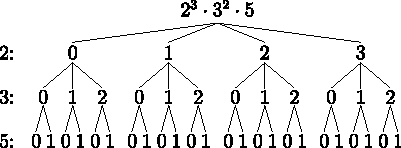
\includegraphics{../graphics/treeDia.pdf}
%\]
%What is going on in this diagram? What do the numbers represent? How
%does it help you count the number of factors of $2^3\cdot 3^2 \cdot
%5$?
%\end{problem}

\end{document}

%\documentclass[handout]{ximera}
\documentclass{ximera}

\usepackage{gensymb}
\usepackage{tabularx}
\usepackage{mdframed}
\usepackage{pdfpages}
%\usepackage{chngcntr}

\let\problem\relax
\let\endproblem\relax

\newcommand{\property}[2]{#1#2}




\newtheoremstyle{SlantTheorem}{\topsep}{\fill}%%% space between body and thm
 {\slshape}                      %%% Thm body font
 {}                              %%% Indent amount (empty = no indent)
 {\bfseries\sffamily}            %%% Thm head font
 {}                              %%% Punctuation after thm head
 {3ex}                           %%% Space after thm head
 {\thmname{#1}\thmnumber{ #2}\thmnote{ \bfseries(#3)}} %%% Thm head spec
\theoremstyle{SlantTheorem}
\newtheorem{problem}{Problem}[]

%\counterwithin*{problem}{section}



%%%%%%%%%%%%%%%%%%%%%%%%%%%%Jenny's code%%%%%%%%%%%%%%%%%%%%

%%% Solution environment
%\newenvironment{solution}{
%\ifhandout\setbox0\vbox\bgroup\else
%\begin{trivlist}\item[\hskip \labelsep\small\itshape\bfseries Solution\hspace{2ex}]
%\par\noindent\upshape\small
%\fi}
%{\ifhandout\egroup\else
%\end{trivlist}
%\fi}
%
%
%%% instructorIntro environment
%\ifhandout
%\newenvironment{instructorIntro}[1][false]%
%{%
%\def\givenatend{\boolean{#1}}\ifthenelse{\boolean{#1}}{\begin{trivlist}\item}{\setbox0\vbox\bgroup}{}
%}
%{%
%\ifthenelse{\givenatend}{\end{trivlist}}{\egroup}{}
%}
%\else
%\newenvironment{instructorIntro}[1][false]%
%{%
%  \ifthenelse{\boolean{#1}}{\begin{trivlist}\item[\hskip \labelsep\bfseries Instructor Notes:\hspace{2ex}]}
%{\begin{trivlist}\item[\hskip \labelsep\bfseries Instructor Notes:\hspace{2ex}]}
%{}
%}
%% %% line at the bottom} 
%{\end{trivlist}\par\addvspace{.5ex}\nobreak\noindent\hung} 
%\fi
%
%


\let\instructorNotes\relax
\let\endinstructorNotes\relax
%%% instructorNotes environment
\ifhandout
\newenvironment{instructorNotes}[1][false]%
{%
\def\givenatend{\boolean{#1}}\ifthenelse{\boolean{#1}}{\begin{trivlist}\item}{\setbox0\vbox\bgroup}{}
}
{%
\ifthenelse{\givenatend}{\end{trivlist}}{\egroup}{}
}
\else
\newenvironment{instructorNotes}[1][false]%
{%
  \ifthenelse{\boolean{#1}}{\begin{trivlist}\item[\hskip \labelsep\bfseries {\Large Instructor Notes: \\} \hspace{\textwidth} ]}
{\begin{trivlist}\item[\hskip \labelsep\bfseries {\Large Instructor Notes: \\} \hspace{\textwidth} ]}
{}
}
{\end{trivlist}}
\fi


%% Suggested Timing
\newcommand{\timing}[1]{{\bf Suggested Timing: \hspace{2ex}} #1}




\hypersetup{
    colorlinks=true,       % false: boxed links; true: colored links
    linkcolor=blue,          % color of internal links (change box color with linkbordercolor)
    citecolor=green,        % color of links to bibliography
    filecolor=magenta,      % color of file links
    urlcolor=cyan           % color of external links
}

\title{Why Does It Work?}
\author{Bart Snapp and Brad Findell}

\outcome{Learning outcome goes here.}

\begin{document}
\begin{abstract}
Abstract goes here.  
\end{abstract}
\maketitle

\label{A:GCDwork}

The Euclidean Algorithm\index{Euclidean Algorithm} is pretty
neat. Let's see if we can figure out \textbf{why} it works. As a gesture of friendship, I'll compute $\gcd(351,153)$:
\begin{align*}
351 &= \boldsymbol{153}\cdot 2 + \boldsymbol{45}\\ 
\boldsymbol{153} &= \boldsymbol{45}\cdot 3 + \boldsymbol{18}\\
\boldsymbol{45} &= \boldsymbol{18}\cdot 2 + \fbox{$\boldsymbol{9}$}\\
18 &= 9\cdot 2 + 0 \qquad \fbox{$\therefore \gcd(351,153) = 9$}
\end{align*}

Let's look at this line-by-line.

\paragraph{The First Line}
\begin{problem}
Since $351 = 153\cdot 2 + 45$, explain why $\gcd(153,45)$ divides $351$.
\end{problem}

\begin{problem}
Since $351 = 153\cdot 2 + 45$, explain why $\gcd(351,153)$ divides $45$.
\end{problem}

\begin{problem}
Since $351 = 153\cdot 2 + 45$, explain why $\gcd(351,153) = \gcd(153,45)$.
\end{problem}


\paragraph{The Second Line}
\begin{problem}
Since $153 = 45\cdot 3 + 18$, explain why $\gcd(45,18)$ divides $153$.
\end{problem}

\begin{problem}
Since $153 = 45\cdot 3 + 18$, explain why $\gcd(153,45)$ divides $18$.
\end{problem}

\begin{problem}
Since $153 = 45\cdot 3 + 18$, explain why $\gcd(153,45) = \gcd(45,18)$.
\end{problem}


\paragraph{The Third Line}
\begin{problem}
Since $45 = 18\cdot 2 + 9$, explain why $\gcd(18,9)$ divides $45$.
\end{problem}

\begin{problem}
Since $45 = 18\cdot 2 + 9$, explain why $\gcd(45,18)$ divides $9$.
\end{problem}

\begin{problem}
Since $45 = 18\cdot 2 + 9$, explain why $\gcd(45,18) = \gcd(18,9)$.
\end{problem}


\paragraph{The Final Line}

\begin{problem}
Why are we done? How do you know that the Euclidean Algorithm
will \textbf{always} terminate?
\end{problem}

\fixnote{New question:  What does the final line look like when the GCD is 1?}  

\end{document}

%\documentclass[handout]{ximera}
\documentclass[nooutcomes]{ximera}

\usepackage{gensymb}
\usepackage{tabularx}
\usepackage{mdframed}
\usepackage{pdfpages}
%\usepackage{chngcntr}

\let\problem\relax
\let\endproblem\relax

\newcommand{\property}[2]{#1#2}




\newtheoremstyle{SlantTheorem}{\topsep}{\fill}%%% space between body and thm
 {\slshape}                      %%% Thm body font
 {}                              %%% Indent amount (empty = no indent)
 {\bfseries\sffamily}            %%% Thm head font
 {}                              %%% Punctuation after thm head
 {3ex}                           %%% Space after thm head
 {\thmname{#1}\thmnumber{ #2}\thmnote{ \bfseries(#3)}} %%% Thm head spec
\theoremstyle{SlantTheorem}
\newtheorem{problem}{Problem}[]

%\counterwithin*{problem}{section}



%%%%%%%%%%%%%%%%%%%%%%%%%%%%Jenny's code%%%%%%%%%%%%%%%%%%%%

%%% Solution environment
%\newenvironment{solution}{
%\ifhandout\setbox0\vbox\bgroup\else
%\begin{trivlist}\item[\hskip \labelsep\small\itshape\bfseries Solution\hspace{2ex}]
%\par\noindent\upshape\small
%\fi}
%{\ifhandout\egroup\else
%\end{trivlist}
%\fi}
%
%
%%% instructorIntro environment
%\ifhandout
%\newenvironment{instructorIntro}[1][false]%
%{%
%\def\givenatend{\boolean{#1}}\ifthenelse{\boolean{#1}}{\begin{trivlist}\item}{\setbox0\vbox\bgroup}{}
%}
%{%
%\ifthenelse{\givenatend}{\end{trivlist}}{\egroup}{}
%}
%\else
%\newenvironment{instructorIntro}[1][false]%
%{%
%  \ifthenelse{\boolean{#1}}{\begin{trivlist}\item[\hskip \labelsep\bfseries Instructor Notes:\hspace{2ex}]}
%{\begin{trivlist}\item[\hskip \labelsep\bfseries Instructor Notes:\hspace{2ex}]}
%{}
%}
%% %% line at the bottom} 
%{\end{trivlist}\par\addvspace{.5ex}\nobreak\noindent\hung} 
%\fi
%
%


\let\instructorNotes\relax
\let\endinstructorNotes\relax
%%% instructorNotes environment
\ifhandout
\newenvironment{instructorNotes}[1][false]%
{%
\def\givenatend{\boolean{#1}}\ifthenelse{\boolean{#1}}{\begin{trivlist}\item}{\setbox0\vbox\bgroup}{}
}
{%
\ifthenelse{\givenatend}{\end{trivlist}}{\egroup}{}
}
\else
\newenvironment{instructorNotes}[1][false]%
{%
  \ifthenelse{\boolean{#1}}{\begin{trivlist}\item[\hskip \labelsep\bfseries {\Large Instructor Notes: \\} \hspace{\textwidth} ]}
{\begin{trivlist}\item[\hskip \labelsep\bfseries {\Large Instructor Notes: \\} \hspace{\textwidth} ]}
{}
}
{\end{trivlist}}
\fi


%% Suggested Timing
\newcommand{\timing}[1]{{\bf Suggested Timing: \hspace{2ex}} #1}




\hypersetup{
    colorlinks=true,       % false: boxed links; true: colored links
    linkcolor=blue,          % color of internal links (change box color with linkbordercolor)
    citecolor=green,        % color of links to bibliography
    filecolor=magenta,      % color of file links
    urlcolor=cyan           % color of external links
}

\title{Prome Factorization}
\author{Bart Snapp and Brad Findell}

\outcome{Learning outcome goes here.}

\begin{document}
\begin{abstract}
  We imagine a system of numbers without unique factorization.
\end{abstract}
\maketitle

\label{A:Prome}

\begin{teachingnote}
In the course, we first assume Euclid's Lemma and use it to prove the Fundamental Theorem of Arithmetic (FTA).  In this activity, both Euclid's Lemma and the FTA fail.

It might help to begin the class with the following questions:  
\begin{itemize}
\item If $7|(ab)$ (where $a$ and $b$ integers), does it follow that $7$ must divide either $a$ or $b$? 
\item If $14|(ab)$ (where $a$ and $b$ integers), does it follow that $14$ must divide either $a$ or $b$? 
\end{itemize}

Through discussion, students should decide that the answers are ``yes'' and ``no,'' respectively, and the reason is that 7 is prime but 14 is not.  Some students should realize that, in the second case, the factors of 2 and 7 (of 14) might be ``split'' between $a$ and $b$.  This realization can be stated as Euclid's Lemma:  

\begin{center}
Suppose $a$ and $b$ are integers and $p$ is prime.  If $p|ab$, then $p|a$ or $p|b$.  
\end{center}

Students are not be responsible for its name.  At this point, we accept it without proof.  

The purpose of questions 1-4 is to see that this ``new'' number system is very much like the integers:  You can always add, subtract, and multiply, but you cannot necessarily divide.  Students can use their reasoning about integers to explain these facts about the system $3\Z$.  

The purpose of questions 5-7 is to notice that both Euclid's Lemma and Unique Factorization fail in this number system.  Some examples:  

$$36 = 3\times 12 = 6\times 6$$
$$72 = 3\times 24=6\times 12$$
\end{teachingnote}


Let's consider a crazy set of numbers---all multiples of $3$. Let's
use the symbol $3\Z$ to denote the set consisting of all multiples of
$3$. As a gesture of friendship, I have written down the first $100$
nonnegative integers in $3\Z$:

\[
\begin{array}{cccccccccc}
0   & 3   & 6   & 9   & 12  & 15  & 18  & 21  & 24  & 27  \\
\\
30  & 33  & 36  & 39  & 42  & 45  & 48  & 51  & 54  & 57  \\
\\
60  & 63  & 66  & 69  & 72  & 75  & 78  & 81  & 84  & 87  \\
\\
90  & 93  & 96  & 99  & 102 & 105 & 108 & 111 & 114 & 117 \\
\\
120 & 123 & 126 & 129 & 132 & 135 & 138 & 141 & 144 & 147 \\
\\
150 & 153 & 156 & 159 & 162 & 165 & 168 & 171 & 174 & 177 \\
\\
180 & 183 & 186 & 189 & 192 & 195 & 198 & 201 & 204 & 207 \\
\\
210 & 213 & 216 & 219 & 222 & 225 & 228 & 231 & 234 & 237 \\
\\
240 & 243 & 246 & 249 & 252 & 255 & 258 & 261 & 264 & 267 \\
\\
270 & 273 & 276 & 279 & 282 & 285 & 288 & 291 & 294 & 297
\end{array}
\]



\begin{problem}
Given any two integers in $3\Z$, will their sum be in $3\Z$? Explain
your reasoning.
\end{problem}

\begin{problem}
Given any two integers in $3\Z$, will their difference be in $3\Z$?
Explain your reasoning.
\end{problem}
\begin{teachingnote}
Yes, but students might need to be reminded that $3\Z$ includes negative integers.  
\end{teachingnote}

\begin{problem}
Given any two integers in $3\Z$, will their product be in $3\Z$?
Explain your reasoning.
\end{problem}

\begin{problem}
Given any two integers in $3\Z$, will their quotient be in $3\Z$?
Explain your reasoning.
\end{problem}

\begin{definition}
Call a positive integer \textbf{prome} in $3\Z$ if it cannot be
expressed as the product of two integers \textit{both} in $3\Z$.
\end{definition}

As an example, I tell you that $6$ is prome number in $3\Z$. You may
object because $6 = 2\cdot 3$, but remember---$2$ is not in $3\Z$!


\begin{problem}
List some of the prome numbers less than $297$.  Hint:  What numbers in $3\Z$ \emph{can} be expressed as a product of two integers \emph{both} in $3\Z$?  
\end{problem}

\begin{problem}
Can you give some sort of algebraic characterization of prome numbers
in $3\Z$? 
\end{problem}

\begin{problem}
Can you find numbers that factor completely into prome numbers in
\textit{two} different ways? How many can you find?
\end{problem}

\end{document}

\newpage
\section{Picture Models for Equivalent Fractions}\label{A:EF}

\begin{teachingnote}

Step 1.  Use the first problem (use paper to show 3/8) to generate the meaning of fraction from the Common Core State Standards:  

\begin{quote}
3.NF.1. Understand a fraction $1/b$ as the quantity formed by $1$ part when a
whole is partitioned into $b$ equal parts; understand a fraction $a/b$ as
the quantity formed by $a$ parts of size $1/b$.

Source:  \url{http://www.corestandards.org/Math/Content/3/NF/A/1/}
\end{quote}


The code 3.NF.1 means ``third grade, number and operations--fractions, standard 1.''  These standards are written to be read by teachers, not students.

Step 2.  Introduce the formal definition of rational number and the set of rational numbers, as in the beginning of section 2.4.  

A rational number can be represented as $a/b$ with integers $a$ and $b$, where $b$ is not $0$.  

Distinguish fraction (a representation) from rational number, highlighting the phrase ``can be'' in the definition.  Have students generate fractions that are not rational numbers as well as rational numbers not represented as fractions.  

Introduce the letter $\Q$ (usually in ``black-board bold'' font) to denote the set of all rational numbers. 

Step 3.  Complete Activity A.16.  The point is to use the meaning of fractions above to explain why fractions are equivalent.  And the approach is ``reasoning generally with specific numbers.'' 

A.16.2.  For $2/3 = 4/6$, some students will be tempted to draw 2/3, draw 4/6 and then say, ``See!''  With this method, it is not clear why the pieces should line up.  Much better to use 2/3 to create 4/6 by cutting each of the thirds into two equal pieces.  

A.16.3.  For $3/6 = 2/4$, some students will be tempted to say ``Because they both equal 1/2.''  To explain why the pieces will have to line up, it is clearer (and more general) to go through a common denominator, such as 12ths or 24ths.  
 
A.16.4.  To show that $a/b = c/d$, generalize the approach from the previous problem:  Thinking of the common denominator $bd$, cut the $a/b$ parts each into $d$ parts.  Then we have $ad$ parts of size $1/(bd)$.  Cut the $c/d$ parts each into $b$ parts.  Then we have $cb$ parts of size $1/(db)$.  For the two fractions to be equal, the $ad$ parts of size $1/(bd)$ must be equal to the $cb$ parts of size $1/(db)$.  

A.16.5.  In the picture from A.16.4, because the parts are the same size (i.e., $1/(bd)$), it must follow that $ad = bc$.  (Argue both directions:  if the fractions are equal, then $ad = bc$;  if $ad = bc$, then the fractions must be equal.)  
\end{teachingnote}

\begin{prob}
Get out a piece of paper and show $\dfrac{3}{8}$.  Explain how you know.  
\end{prob}

\begin{prob}
Compare the following fractions.  Explain how you know:
\begin{enumerate}
\item $\frac{3}{5} \qquad \frac{4}{5}$
\item $\frac{3}{7} \qquad \frac{3}{8}$
\item $\frac{3}{7} \qquad \frac{5}{9}$
\item $\frac{6}{7} \qquad \frac{7}{8}$
\item $\frac{12}{11} \qquad \frac{13}{14}$
\end{enumerate}
\begin{teachingnote}
In the above comparison problems, highlight common denominator and common numerator strategies.  Also highlight comparing to benchmarks such as $1/2$ or $1$. 
\end{teachingnote}
\end{prob}

\begin{prob} 
Draw pictures to explain why:
\[
\frac{2}{3} = \frac{4}{6}
\]
Explain how your pictures show this.
\end{prob}


\begin{prob} 
Draw pictures to explain why:
\[
\frac{3}{6} = \frac{2}{4}
\]
Explain how your pictures show this.
\end{prob}



\begin{prob} 
Given equivalent fractions with $0< a\le b$ and $0 < c\le d$:
\[
\frac{a}{b} = \frac{c}{d}
\]
Give a procedure for representing this equation with pictures.
\end{prob}


\begin{prob} 
Explain, without cross-multiplication, why if $0< a\le b$ and $0 < c\le d$:
\[
\frac{a}{b} = \frac{c}{d}\qquad \text{if and only if}\qquad ad = bc
\]
Feel free to use pictures as part of your explanation.
\end{prob}

\newpage
\section{Picture Models for Fraction Operations}\label{A:FO}
\begin{prob} 
Draw pictures that model:
\[
\frac{1}{5} + \frac{2}{5} = \frac{3}{5}
\]
Explain how your pictures show this. Write a story problem whose
solution is given by the expression above.
\end{prob}

\begin{prob} 
Draw pictures that model:
\[
\frac{2}{3} + \frac{1}{4} = \frac{11}{12}
\]
Explain how your pictures model this equation. Be sure to carefully
explain how common denominators are represented in your
pictures. Write a story problem whose solution is given by the
expression above.
\end{prob}

\begin{prob} 
Given $0<a\le b$ and $0<c\le d$, explain how to draw pictures
that model the sum:
\[
\frac{a}{b} + \frac{c}{d}
\]
Use pictures to find this sum and carefully explain how common
denominators are represented in your pictures.
\end{prob}

% The following problems have been replaced by a new activity about fraction multiplication
%
%\begin{prob} 
%Given positive integers $a$ and $b$, explain how to draw pictures that
%model the product $a\cdot b$---give an example of your process.
%\end{prob}
%
%\begin{prob} 
%Draw pictures that model:
%\[
%\frac{4}{5} \cdot \frac{2}{3} = \frac{8}{15}
%\]
%Explain how your pictures model this equation. Write a story problem
%whose solution is given by the expression above. Does your story work with 
%\[
%\frac{7}{5} \cdot \frac{2}{3} = \frac{14}{15}?
%\]
%\end{prob}
%
%\begin{prob} 
%Given $0<a\le b$ and $0<c\le d$, explain how to draw pictures
%that model the product:
%\[
%\frac{a}{b} \cdot \frac{c}{d}
%\]
%Use pictures to find this product and explain how this product is shown
%in your pictures---give an example of your process.
%\end{prob}

%\documentclass[handout]{ximera}
\documentclass[nooutcomes]{ximera}

\usepackage{gensymb}
\usepackage{tabularx}
\usepackage{mdframed}
\usepackage{pdfpages}
%\usepackage{chngcntr}

\let\problem\relax
\let\endproblem\relax

\newcommand{\property}[2]{#1#2}




\newtheoremstyle{SlantTheorem}{\topsep}{\fill}%%% space between body and thm
 {\slshape}                      %%% Thm body font
 {}                              %%% Indent amount (empty = no indent)
 {\bfseries\sffamily}            %%% Thm head font
 {}                              %%% Punctuation after thm head
 {3ex}                           %%% Space after thm head
 {\thmname{#1}\thmnumber{ #2}\thmnote{ \bfseries(#3)}} %%% Thm head spec
\theoremstyle{SlantTheorem}
\newtheorem{problem}{Problem}[]

%\counterwithin*{problem}{section}



%%%%%%%%%%%%%%%%%%%%%%%%%%%%Jenny's code%%%%%%%%%%%%%%%%%%%%

%%% Solution environment
%\newenvironment{solution}{
%\ifhandout\setbox0\vbox\bgroup\else
%\begin{trivlist}\item[\hskip \labelsep\small\itshape\bfseries Solution\hspace{2ex}]
%\par\noindent\upshape\small
%\fi}
%{\ifhandout\egroup\else
%\end{trivlist}
%\fi}
%
%
%%% instructorIntro environment
%\ifhandout
%\newenvironment{instructorIntro}[1][false]%
%{%
%\def\givenatend{\boolean{#1}}\ifthenelse{\boolean{#1}}{\begin{trivlist}\item}{\setbox0\vbox\bgroup}{}
%}
%{%
%\ifthenelse{\givenatend}{\end{trivlist}}{\egroup}{}
%}
%\else
%\newenvironment{instructorIntro}[1][false]%
%{%
%  \ifthenelse{\boolean{#1}}{\begin{trivlist}\item[\hskip \labelsep\bfseries Instructor Notes:\hspace{2ex}]}
%{\begin{trivlist}\item[\hskip \labelsep\bfseries Instructor Notes:\hspace{2ex}]}
%{}
%}
%% %% line at the bottom} 
%{\end{trivlist}\par\addvspace{.5ex}\nobreak\noindent\hung} 
%\fi
%
%


\let\instructorNotes\relax
\let\endinstructorNotes\relax
%%% instructorNotes environment
\ifhandout
\newenvironment{instructorNotes}[1][false]%
{%
\def\givenatend{\boolean{#1}}\ifthenelse{\boolean{#1}}{\begin{trivlist}\item}{\setbox0\vbox\bgroup}{}
}
{%
\ifthenelse{\givenatend}{\end{trivlist}}{\egroup}{}
}
\else
\newenvironment{instructorNotes}[1][false]%
{%
  \ifthenelse{\boolean{#1}}{\begin{trivlist}\item[\hskip \labelsep\bfseries {\Large Instructor Notes: \\} \hspace{\textwidth} ]}
{\begin{trivlist}\item[\hskip \labelsep\bfseries {\Large Instructor Notes: \\} \hspace{\textwidth} ]}
{}
}
{\end{trivlist}}
\fi


%% Suggested Timing
\newcommand{\timing}[1]{{\bf Suggested Timing: \hspace{2ex}} #1}




\hypersetup{
    colorlinks=true,       % false: boxed links; true: colored links
    linkcolor=blue,          % color of internal links (change box color with linkbordercolor)
    citecolor=green,        % color of links to bibliography
    filecolor=magenta,      % color of file links
    urlcolor=cyan           % color of external links
}

\title{Fraction Multiplication}
\author{Bart Snapp and Brad Findell}

\outcome{Learning outcome goes here.}

\begin{document}
\begin{abstract}
  We think about what multiplication of fractions means.
\end{abstract}
\maketitle

\label{A:fractionMultiplication}

\begin{problem}
Suppose $x$ and $y$ are counting numbers.  
\begin{enumerate}
\item What is our convention for the meaning of $xy$ as repeated addition?  
\item In our convention for the meaning of the product $xy$, which letter describes 
\emph{how many groups} and which letter describes \emph{how many in one group}? 
\item In the product $xy$, the $x$ is called the \emph{multiplier} and $y$ is called the \emph{multiplicand}.  
Use these words to describe the meaning of $xy$ as repeated addition. 
\end{enumerate}
\end{problem}

\vspace{1in}

\begin{problem}
In the Common Core State Standards, fractions and fraction operations are built from \emph{unit fractions}, which are fractions with a $1$ in the numerator.  The meaning of a fraction $\frac{a}{b}$ involves three steps: (1) determining the whole; (2) describing the meaning of $\frac{1}{b}$; and (3) describe the meaning of the fraction $\frac{a}{b}$.  Use pictures to illustrate these three steps for the fraction
$\frac{3}{5}$.  
\end{problem}

\vspace{1in}

\begin{problem}
Now we combine the ideas from the previous two problems to describe meanings for simple multiplication of fractions.  
\begin{enumerate}
\item Without computing the result, describe the meaning of the product $5 \times \frac{1}{3}$.
\item Without computing the result, describe the meaning of the product $\frac{1}{3}\times 5$.
\item Without using the commutativity of multiplication (which we have not established for fractions), 
use these meanings and pictures to explain what the products should be. 
\end{enumerate}
\end{problem}

\vspace{1in}

\subsection*{Area Models}
\begin{problem}
Beginning with a unit square, use an area model to illustrate the following:  
\begin{enumerate}
\item $\frac{1}{3}\times \frac{1}{4}$ 
\item $\frac{7}{3}\times \frac{5}{4}$
\end{enumerate}
\end{problem}

\vspace{1.5in}
\
\begin{problem}
When computing $2\frac{1}{3}\times 3\frac{2}{5}$, Byron says that the answer is $6\frac{2}{15}$.  
\begin{enumerate}
\item Explain Byron's method. 
\item How do you know that he is incorrect?  
\item Use what is right about his method to show what he is missing. 
\end{enumerate}
\end{problem}

\end{document}

\newpage
\section{Flour Power}\label{A:FlourPower}

\begin{prob} 
Suppose a cookie recipe calls for $2$ cups of flour. If you have $6$
cups of flour total, how many batches of cookies can you make?
\begin{enumerate}
\item Draw a picture representing the situation, and use pictures to solve the problem.
\item Identify whether the problem is asking ``How many groups?'' or ``How many in one group?'' or something else entirely.
\item You find another recipe that calls for $1\frac{1}{2}$ cups per batch. If you have $6$ cups of flour, how many batches of these cookies can you make?  Again use pictures to solve the problem.
\item Somebody once told you that ``to divide fractions, you invert and
multiply.'' Discuss how this rule is manifested in this problem.
\end{enumerate}
\end{prob}

\begin{prob} 
You have $2$ snazzy stainless steel containers (both the same size), which hold a total of
$6$ cups of flour. How many cups of flour does $1$ container hold?
\begin{enumerate}
\item Draw a picture representing the situation, and use pictures to solve the problem.
\item Identify whether the problem is asking ``How many groups?'' or ``How many in one group?'' or something else entirely.
\item It turned out that the 6 cups of flour filled exactly $1\frac{1}{2}$ of your containers.  How many cups of flour does $1$ container hold?  Again use pictures to solve the problem.
\item Somebody once told you that ``to divide fractions, you invert and
multiply.'' Discuss how this rule is manifested in this problem.
\end{enumerate}
\end{prob}


%\begin{prob} 
%Now you have $3$ beautiful decorative bowls, which hold a total of
%$1/2$ cup of flour. How many cups of flour does $1$ decorative bowl
%hold?
%\begin{enumerate}
%\item Draw a picture representing the situation, and use your picture to solve the problem.
%\item Identify whether the problem is asking ``How many groups?'' or ``How many in one group?'' or something else entirely.
%\item Somebody once told you that ``to divide fractions, you invert and
%multiply.'' Discuss how this rule is manifested in this problem.
%\end{enumerate}
%\end{prob}
%

\newpage
\section{Picture Yourself Dividing}


We want to understand how to visualize 
\[
\frac{a}{b} \div \frac{c}{d}
\]
Let's see if we can ease into this.

\begin{prob}
Draw a picture that shows how to compute:
\[
10\div 5
\]
Explain how your picture could be redrawn for other similar
numbers. Write two story problems solved by this expression, one
asking for ``how many groups'' and the other asking for ``how many in
one group.''
\end{prob}

\begin{teachingnote}
Some students will write story problems that make sense only for whole number divisors, dividends, quotients, and remainders.  These problems are (mentally) challenging to imagine with non-integer quantities.  Spend some class discussion on discrete vs. continuous quantities, and talk about how continuous quantities are crucial for thinking about fraction division.  
\end{teachingnote}

\begin{prob}
Try to use a similar process to the one you used in the first problem
to draw a picture that shows how to compute:
\[
\frac{1}{4} \div 3
\]
Explain how your picture could be redrawn for other similar numbers.
Write two story problems solved by this expression, one asking for
``how many groups'' and the other asking for ``how many in one
group.''
\end{prob}


\begin{prob}
Try to use a similar process to the one you used in the first two problems
to draw a picture that shows how to compute:
\[
3 \div \frac{1}{4}
\]
Explain how your picture could be redrawn for other similar numbers.
Write two story problems solved by this expression, one asking for
``how many groups'' and the other asking for ``how many in one
group.''
\end{prob}

\fixnote{Also incorporate $1\frac{3}{4}\div \frac{1}{2}$, showing a common incorrect story problem.}

\begin{prob}
Try to use a similar process to the one you used in the first three problems
to draw a picture that shows how to compute:
\[
\frac{7}{5} \div \frac{3}{4}
\]
Explain how your picture could be redrawn for other similar numbers.
Write two story problems solved by this expression, one asking for
``how many groups'' and the other asking for ``how many in each
group.''
\end{prob}

\begin{prob}
Explain how to draw pictures to visualize:
\[
\frac{a}{b} \div \frac{c}{d}
\]
\end{prob}

\begin{prob}
Use pictures to explain why:
\[
\frac{a}{b} \div \frac{c}{d} = \frac{a}{b} \cdot \frac{d}{c}
\]
\end{prob}

\newpage
\section{Cross Something-ing}\label{A:CrossSomething}


\begin{prob} 
What might someone call the following statements:
\begin{enumerate}
\item $\dfrac{a}{b} = \dfrac{c}{d} \Rightarrow ad = bc$
\item $\dfrac{a}{b}\cdot \dfrac{b}{c} = \dfrac{a}{c}$
\item $\dfrac{a}{b}\div \dfrac{c}{d} = \dfrac{ad}{bc}$
\item $\dfrac{a}{b} +\dfrac{c}{d} = \dfrac{ad+bc}{bd}$
\item $ad < bc \Rightarrow \dfrac{a}{b} < \dfrac{c}{d}$
\item $ad < bc \Rightarrow \dfrac{c}{d} < \dfrac{a}{b}$
\end{enumerate}
\end{prob}

\begin{prob}
Which of the above statements are true? What specific name might you
use to describe them?
\end{prob}

\begin{prob} 
Use pictures to help explain why the true statements above are true
and give counterexamples showing that the false statements are false.
\end{prob}


\begin{prob} 
Can you think of other statements that should be grouped with those
above?
\end{prob}

\begin{prob}
If mathematics is a subject where you should strive to ``say what you
mean and mean what you say,'' what issue might arise with
cross-multiplication?
\end{prob}


%\documentclass[handout]{ximera}
\documentclass[nooutcomes]{ximera}

\usepackage{gensymb}
\usepackage{tabularx}
\usepackage{mdframed}
\usepackage{pdfpages}
%\usepackage{chngcntr}

\let\problem\relax
\let\endproblem\relax

\newcommand{\property}[2]{#1#2}




\newtheoremstyle{SlantTheorem}{\topsep}{\fill}%%% space between body and thm
 {\slshape}                      %%% Thm body font
 {}                              %%% Indent amount (empty = no indent)
 {\bfseries\sffamily}            %%% Thm head font
 {}                              %%% Punctuation after thm head
 {3ex}                           %%% Space after thm head
 {\thmname{#1}\thmnumber{ #2}\thmnote{ \bfseries(#3)}} %%% Thm head spec
\theoremstyle{SlantTheorem}
\newtheorem{problem}{Problem}[]

%\counterwithin*{problem}{section}



%%%%%%%%%%%%%%%%%%%%%%%%%%%%Jenny's code%%%%%%%%%%%%%%%%%%%%

%%% Solution environment
%\newenvironment{solution}{
%\ifhandout\setbox0\vbox\bgroup\else
%\begin{trivlist}\item[\hskip \labelsep\small\itshape\bfseries Solution\hspace{2ex}]
%\par\noindent\upshape\small
%\fi}
%{\ifhandout\egroup\else
%\end{trivlist}
%\fi}
%
%
%%% instructorIntro environment
%\ifhandout
%\newenvironment{instructorIntro}[1][false]%
%{%
%\def\givenatend{\boolean{#1}}\ifthenelse{\boolean{#1}}{\begin{trivlist}\item}{\setbox0\vbox\bgroup}{}
%}
%{%
%\ifthenelse{\givenatend}{\end{trivlist}}{\egroup}{}
%}
%\else
%\newenvironment{instructorIntro}[1][false]%
%{%
%  \ifthenelse{\boolean{#1}}{\begin{trivlist}\item[\hskip \labelsep\bfseries Instructor Notes:\hspace{2ex}]}
%{\begin{trivlist}\item[\hskip \labelsep\bfseries Instructor Notes:\hspace{2ex}]}
%{}
%}
%% %% line at the bottom} 
%{\end{trivlist}\par\addvspace{.5ex}\nobreak\noindent\hung} 
%\fi
%
%


\let\instructorNotes\relax
\let\endinstructorNotes\relax
%%% instructorNotes environment
\ifhandout
\newenvironment{instructorNotes}[1][false]%
{%
\def\givenatend{\boolean{#1}}\ifthenelse{\boolean{#1}}{\begin{trivlist}\item}{\setbox0\vbox\bgroup}{}
}
{%
\ifthenelse{\givenatend}{\end{trivlist}}{\egroup}{}
}
\else
\newenvironment{instructorNotes}[1][false]%
{%
  \ifthenelse{\boolean{#1}}{\begin{trivlist}\item[\hskip \labelsep\bfseries {\Large Instructor Notes: \\} \hspace{\textwidth} ]}
{\begin{trivlist}\item[\hskip \labelsep\bfseries {\Large Instructor Notes: \\} \hspace{\textwidth} ]}
{}
}
{\end{trivlist}}
\fi


%% Suggested Timing
\newcommand{\timing}[1]{{\bf Suggested Timing: \hspace{2ex}} #1}




\hypersetup{
    colorlinks=true,       % false: boxed links; true: colored links
    linkcolor=blue,          % color of internal links (change box color with linkbordercolor)
    citecolor=green,        % color of links to bibliography
    filecolor=magenta,      % color of file links
    urlcolor=cyan           % color of external links
}

\title{Hundredths Grids for Rational Numbers}
\author{Bart Snapp and Brad Findell}

\outcome{Learning outcome goes here.}

\begin{document}
\begin{abstract}
  We convert fractions into decimals using hundredths grids.
\end{abstract}
\maketitle

\label{A:hundredthsGrids}


When a $10\times 10$ square is taken to be $1$ whole, it can be used as a ``hundredths grid'' 
to represent fractions and decimals between $0$ and $1$. For example, one of the grids below 
is shaded to represent $\frac{21}{100}$.
\begin{image}
  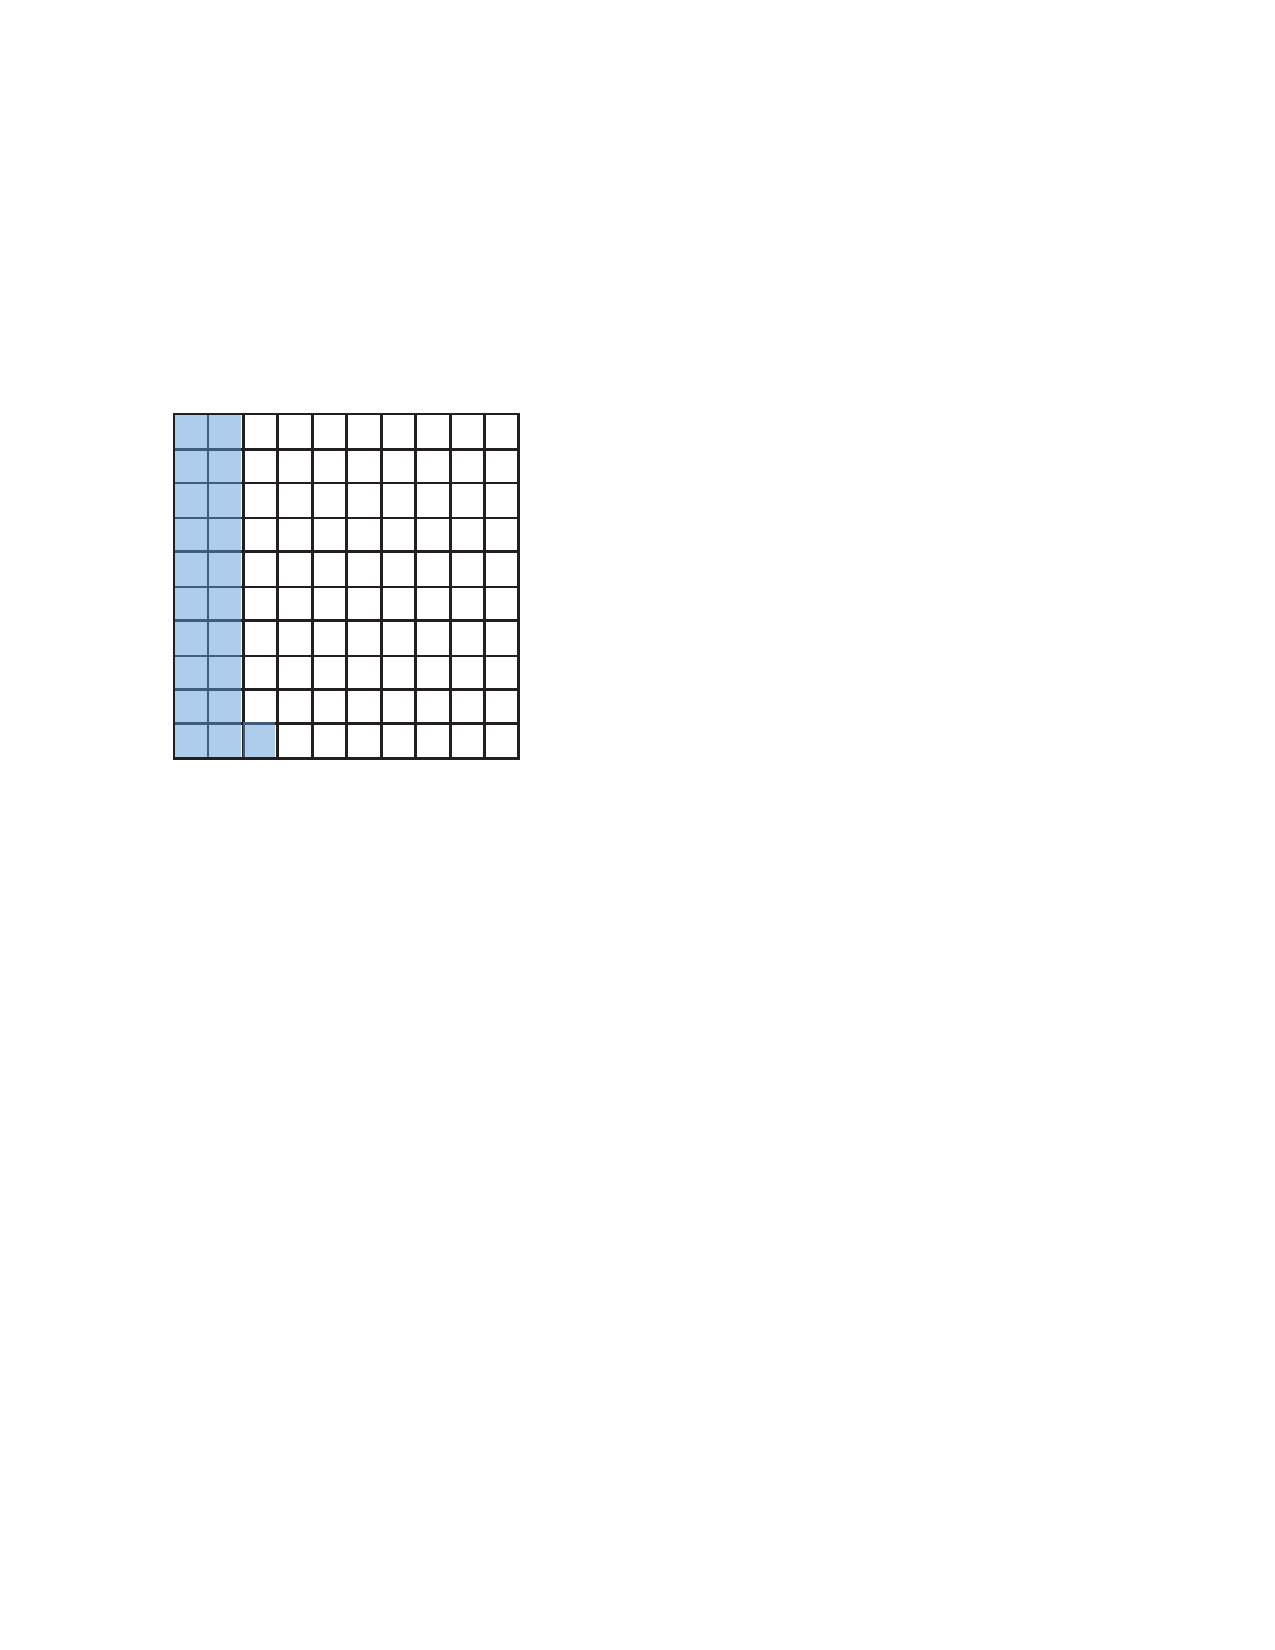
\includegraphics{../graphics/hundredthsGridSample}
\end{image}


\begin{problem}
  Shade the hundredths grid below to show $\frac{3}{20}$. Use your
  shading to determine a decimal equivalent for each fraction.
  \begin{image}
    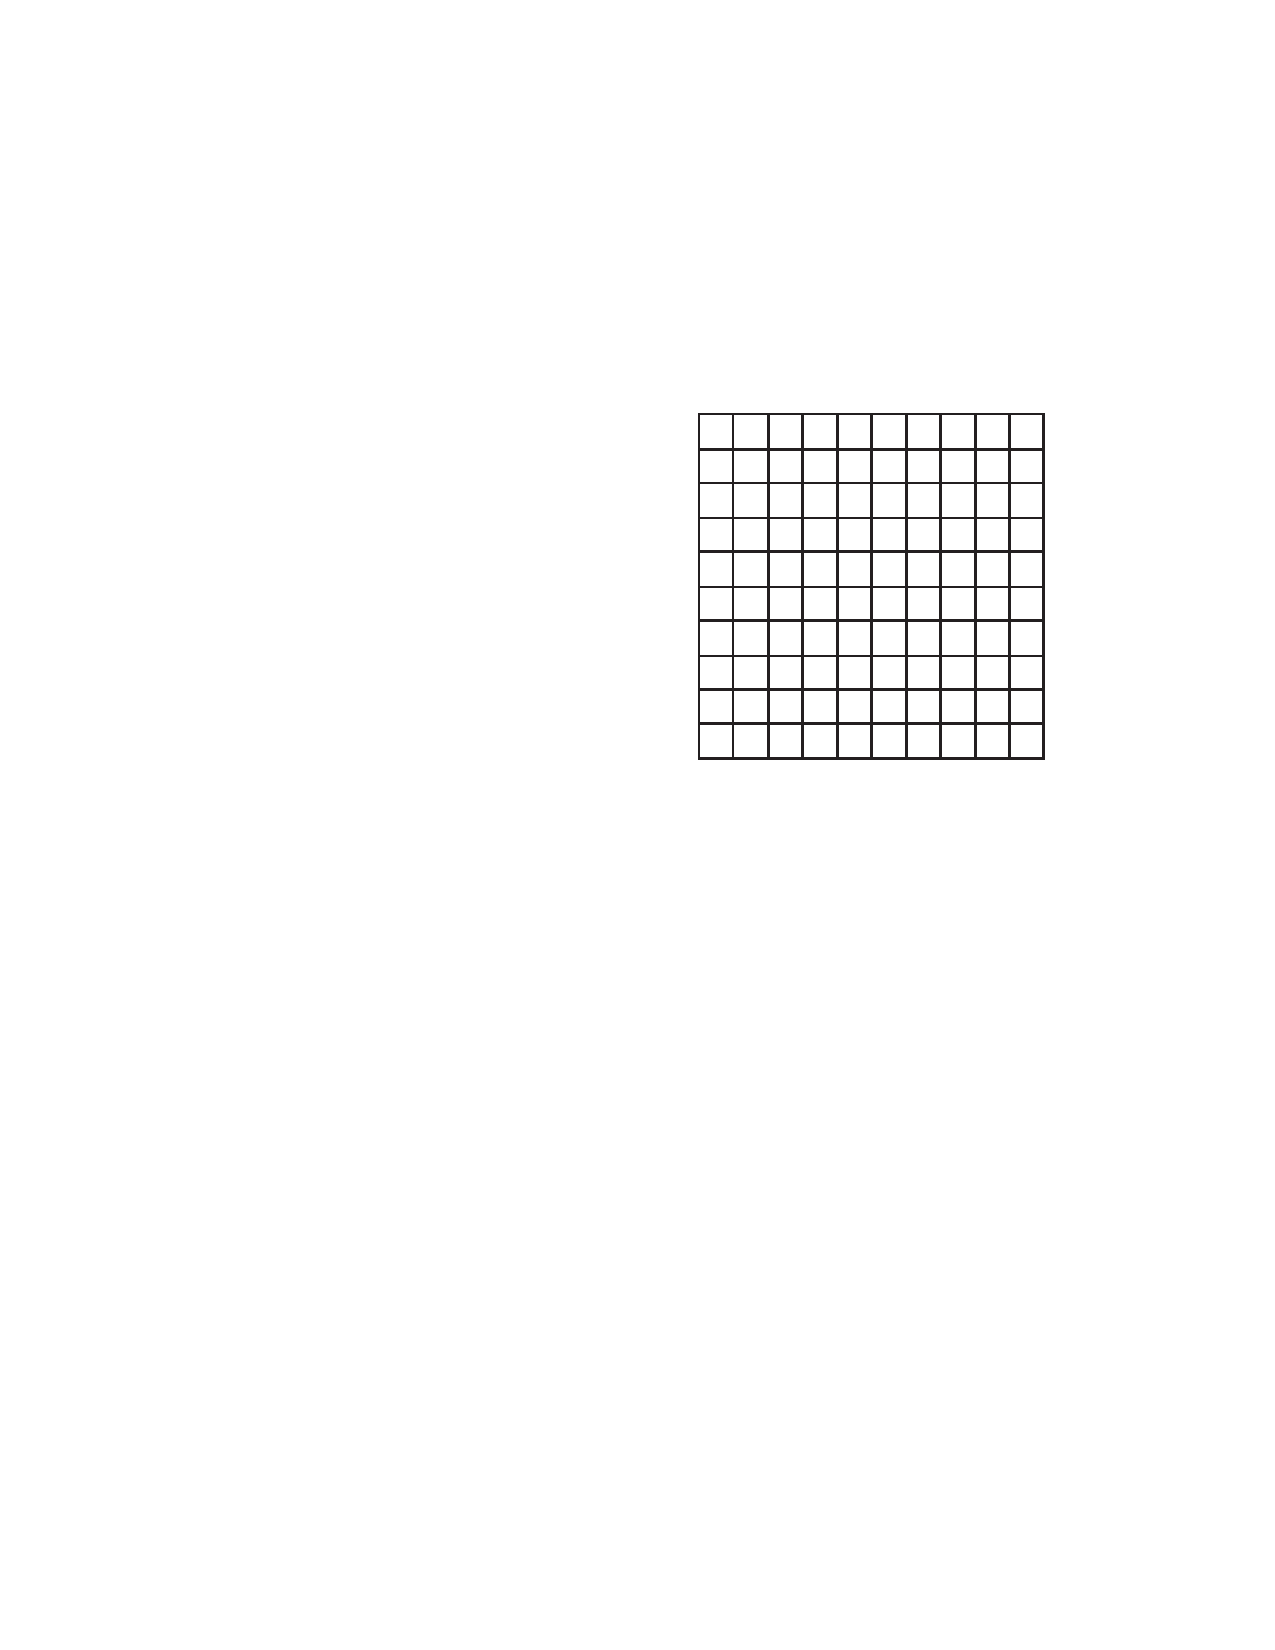
\includegraphics{../graphics/hundredthsGrid0.pdf}
  \end{image}
\end{problem}



\begin{problem}
  Shade the hundredths grid below to show $\frac{1}{8}$. Use your
  shading to determine a decimal equivalent for each fraction.
  \begin{image}
    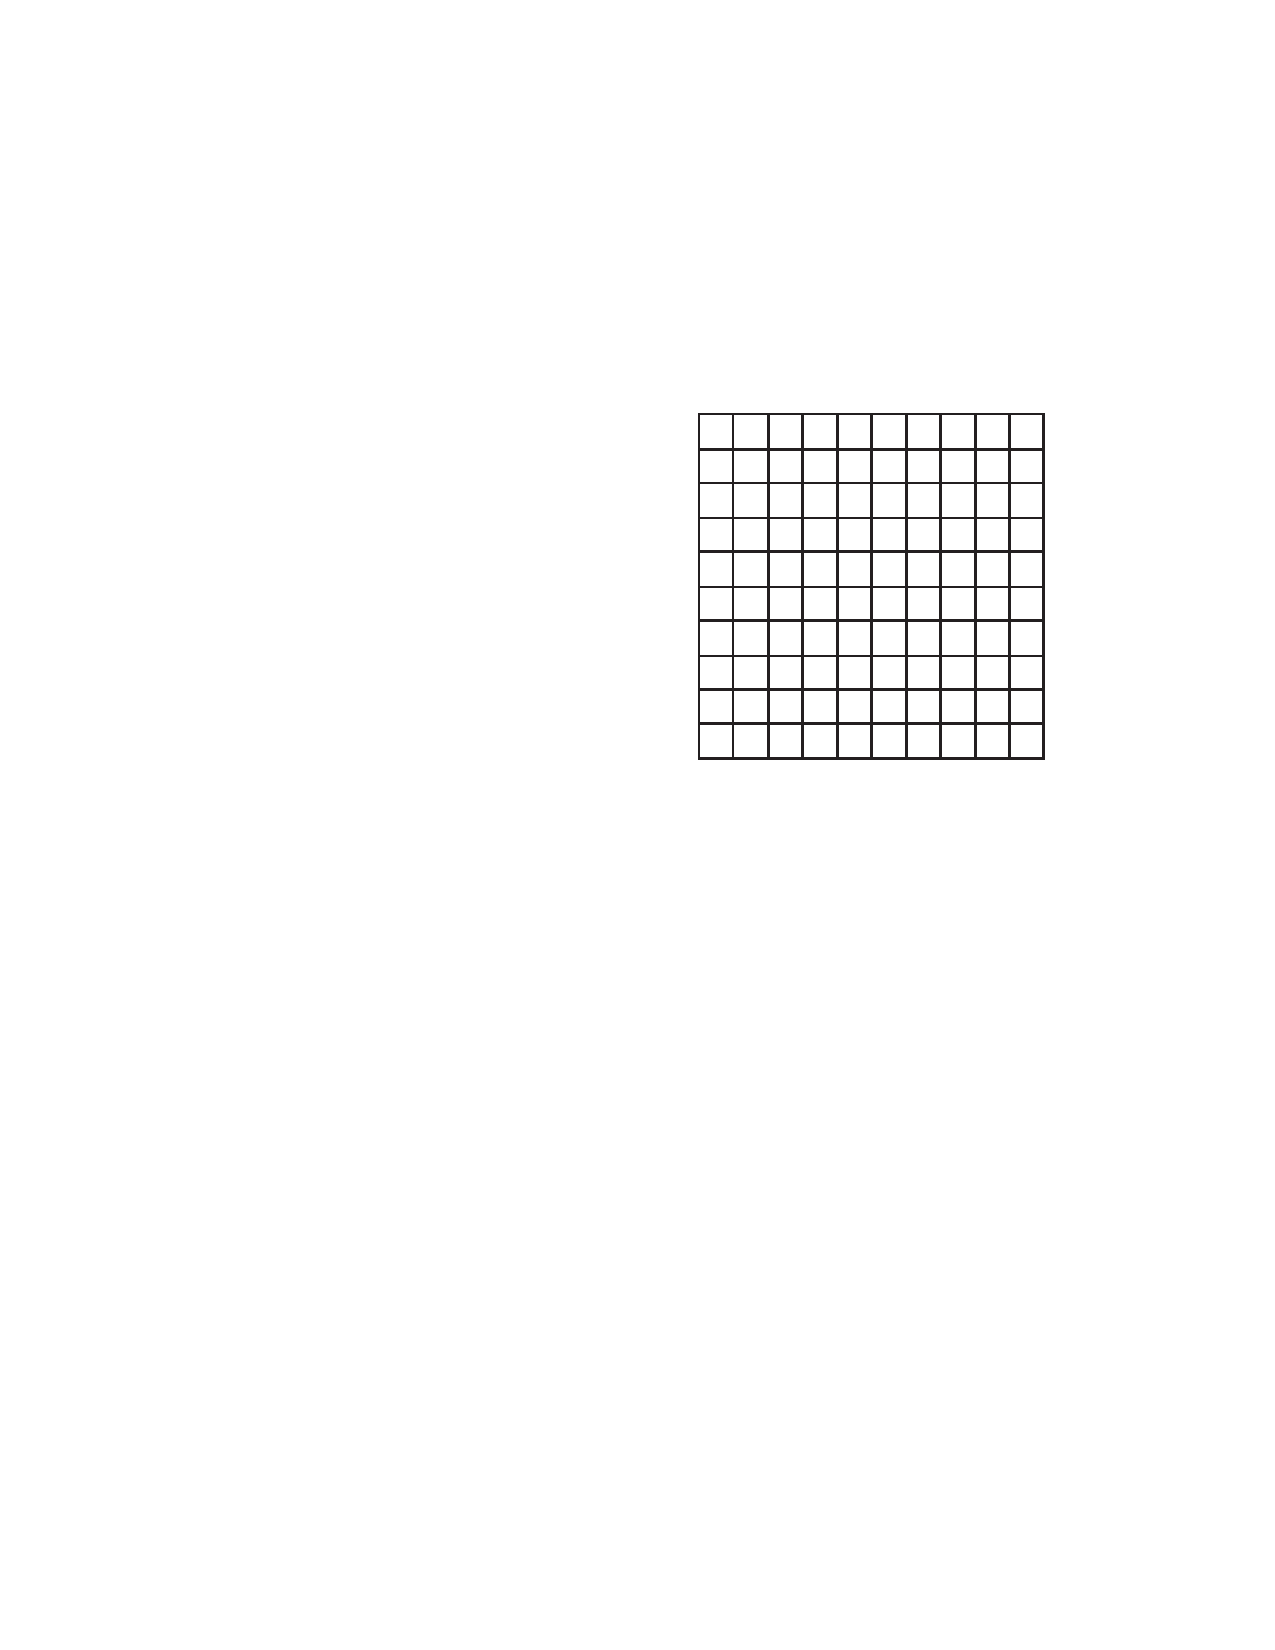
\includegraphics{../graphics/hundredthsGrid0.pdf}
  \end{image}
\end{problem}



\begin{problem}
  Shade the hundredths grid below to show $\frac{1}{6}$. Use your
  shading to determine a decimal equivalent for each fraction.
  \begin{image}
    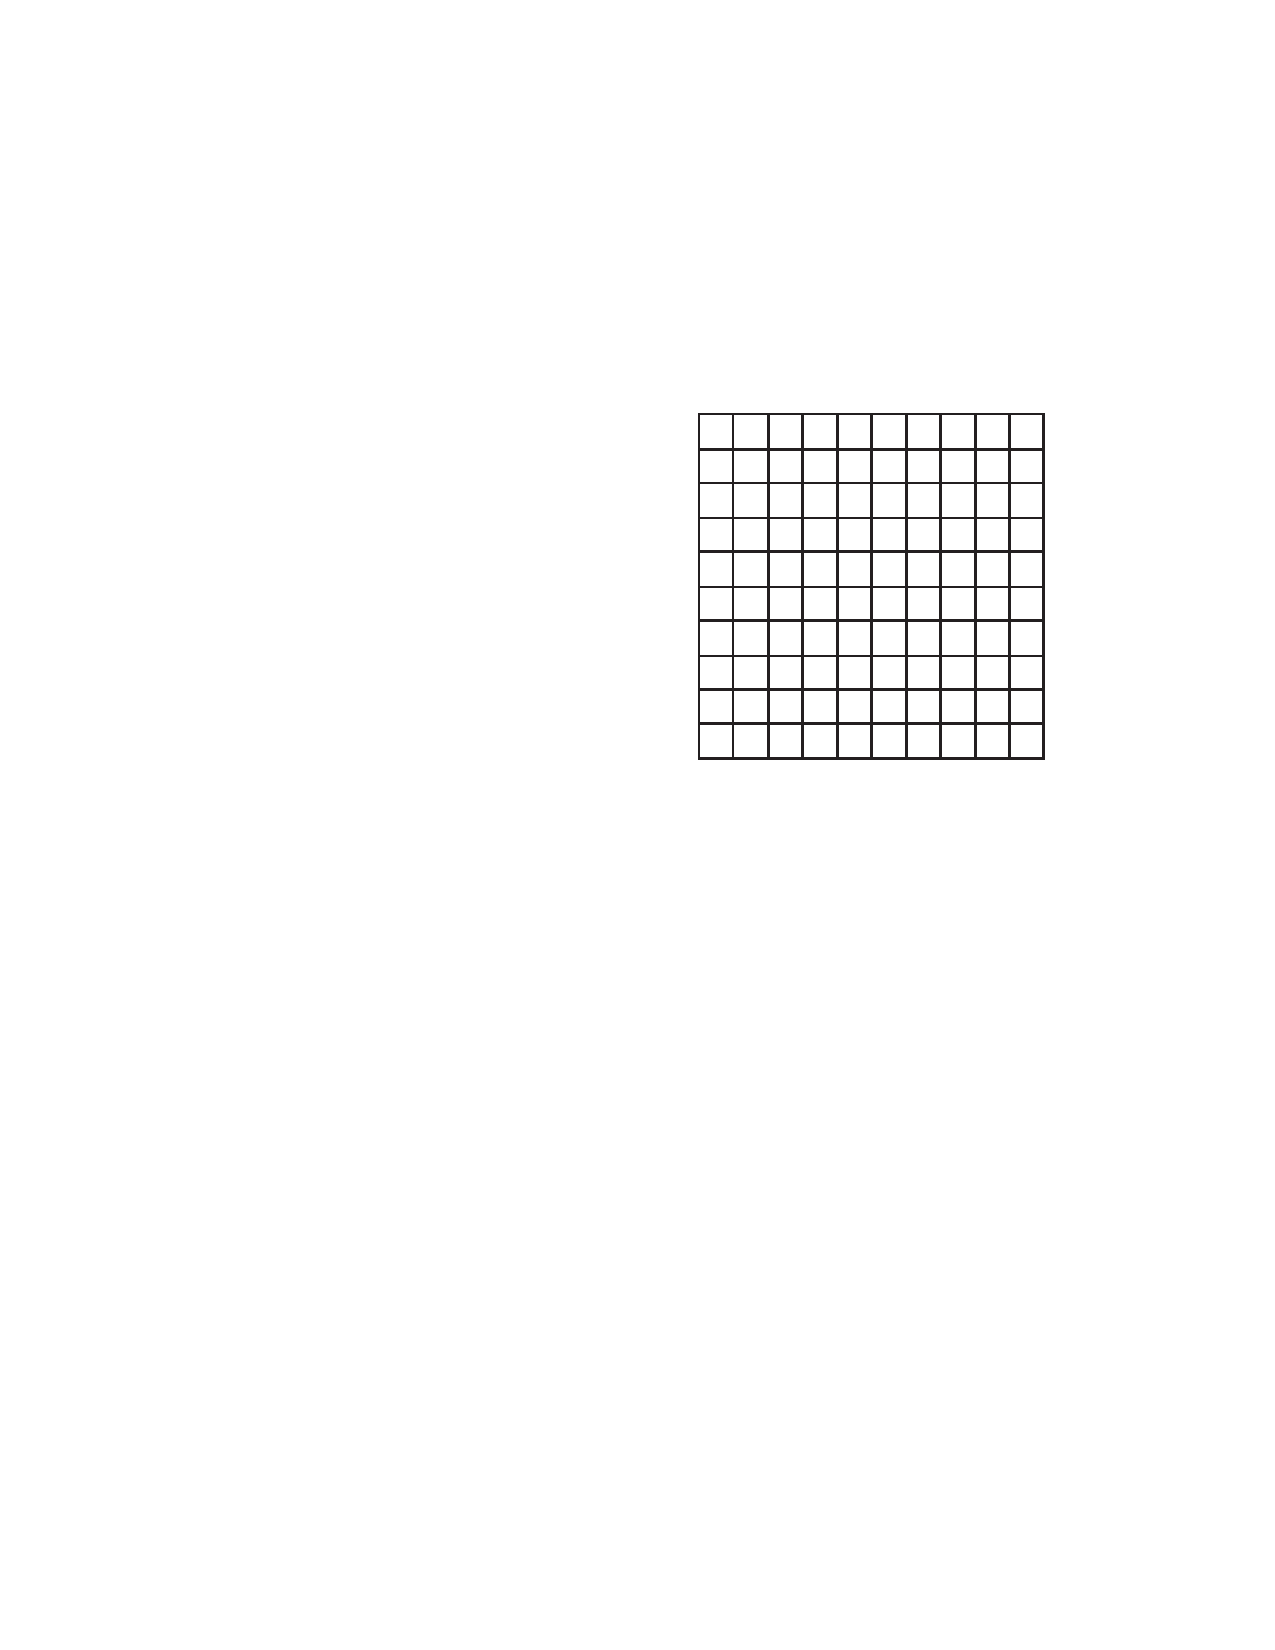
\includegraphics{../graphics/hundredthsGrid0.pdf}
  \end{image}
\end{problem}


\begin{problem}
  Shade the hundredths grid below to show $\frac{7}{12}$. Use your
  shading to determine a decimal equivalent for each fraction.
  \begin{image}
    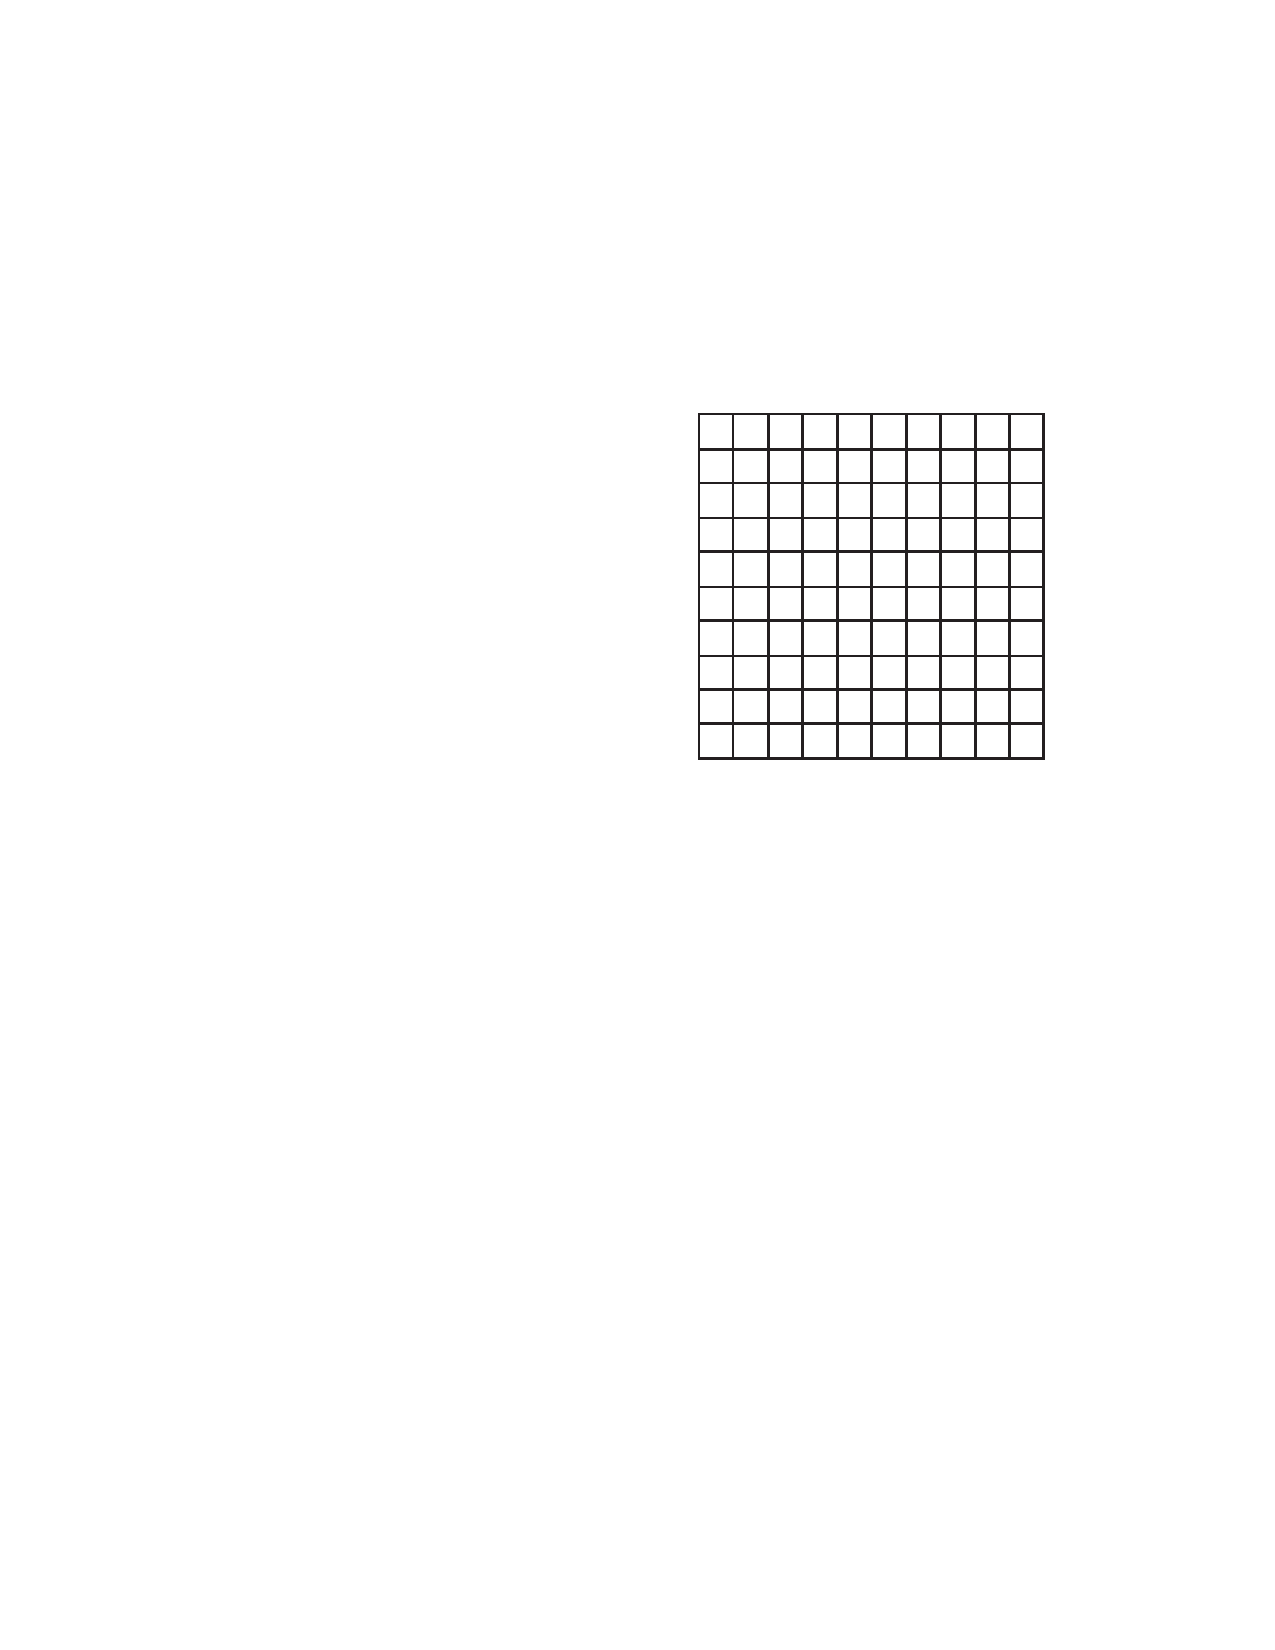
\includegraphics{../graphics/hundredthsGrid0.pdf}
  \end{image}
\end{problem}
  

\end{document}

%\documentclass[handout]{ximera}
\documentclass{ximera}

\usepackage{gensymb}
\usepackage{tabularx}
\usepackage{mdframed}
\usepackage{pdfpages}
%\usepackage{chngcntr}

\let\problem\relax
\let\endproblem\relax

\newcommand{\property}[2]{#1#2}




\newtheoremstyle{SlantTheorem}{\topsep}{\fill}%%% space between body and thm
 {\slshape}                      %%% Thm body font
 {}                              %%% Indent amount (empty = no indent)
 {\bfseries\sffamily}            %%% Thm head font
 {}                              %%% Punctuation after thm head
 {3ex}                           %%% Space after thm head
 {\thmname{#1}\thmnumber{ #2}\thmnote{ \bfseries(#3)}} %%% Thm head spec
\theoremstyle{SlantTheorem}
\newtheorem{problem}{Problem}[]

%\counterwithin*{problem}{section}



%%%%%%%%%%%%%%%%%%%%%%%%%%%%Jenny's code%%%%%%%%%%%%%%%%%%%%

%%% Solution environment
%\newenvironment{solution}{
%\ifhandout\setbox0\vbox\bgroup\else
%\begin{trivlist}\item[\hskip \labelsep\small\itshape\bfseries Solution\hspace{2ex}]
%\par\noindent\upshape\small
%\fi}
%{\ifhandout\egroup\else
%\end{trivlist}
%\fi}
%
%
%%% instructorIntro environment
%\ifhandout
%\newenvironment{instructorIntro}[1][false]%
%{%
%\def\givenatend{\boolean{#1}}\ifthenelse{\boolean{#1}}{\begin{trivlist}\item}{\setbox0\vbox\bgroup}{}
%}
%{%
%\ifthenelse{\givenatend}{\end{trivlist}}{\egroup}{}
%}
%\else
%\newenvironment{instructorIntro}[1][false]%
%{%
%  \ifthenelse{\boolean{#1}}{\begin{trivlist}\item[\hskip \labelsep\bfseries Instructor Notes:\hspace{2ex}]}
%{\begin{trivlist}\item[\hskip \labelsep\bfseries Instructor Notes:\hspace{2ex}]}
%{}
%}
%% %% line at the bottom} 
%{\end{trivlist}\par\addvspace{.5ex}\nobreak\noindent\hung} 
%\fi
%
%


\let\instructorNotes\relax
\let\endinstructorNotes\relax
%%% instructorNotes environment
\ifhandout
\newenvironment{instructorNotes}[1][false]%
{%
\def\givenatend{\boolean{#1}}\ifthenelse{\boolean{#1}}{\begin{trivlist}\item}{\setbox0\vbox\bgroup}{}
}
{%
\ifthenelse{\givenatend}{\end{trivlist}}{\egroup}{}
}
\else
\newenvironment{instructorNotes}[1][false]%
{%
  \ifthenelse{\boolean{#1}}{\begin{trivlist}\item[\hskip \labelsep\bfseries {\Large Instructor Notes: \\} \hspace{\textwidth} ]}
{\begin{trivlist}\item[\hskip \labelsep\bfseries {\Large Instructor Notes: \\} \hspace{\textwidth} ]}
{}
}
{\end{trivlist}}
\fi


%% Suggested Timing
\newcommand{\timing}[1]{{\bf Suggested Timing: \hspace{2ex}} #1}




\hypersetup{
    colorlinks=true,       % false: boxed links; true: colored links
    linkcolor=blue,          % color of internal links (change box color with linkbordercolor)
    citecolor=green,        % color of links to bibliography
    filecolor=magenta,      % color of file links
    urlcolor=cyan           % color of external links
}

\title{Shampoo, Rinse, \dots}
\author{Bart Snapp and Brad Findell}

\outcome{Learning outcome goes here.}

\begin{document}
\begin{abstract}
Abstract goes here.  
\end{abstract}
\maketitle

\label{A:Shampoo}
\index{repeating decimal}
\index{terminating decimal}

\fixnote{Table doesn't look great.  Cross-references are not working.}
We're going to investigate the following question: If $a$ and $b$ are
integers with $b \ne 0$, what can you say about the decimal
representation of $a/b$? 

As a middle school teacher, you should know from memory the decimal equivalents of many fractions, and 
you should be able to compute others quickly in your head.  Use this activity to hone this skill, and use your calculator 
as backup support.  

\begin{problem}\label{AR:exp} 
Complete the following table.  For type, write ``T'' for ``Terminating,'' and use other letters for other types you observe.  

%\begin{multicols}{2}

\renewcommand{\arraystretch}{2}
\begin{tabular}{l}
$\begin{array}{|c|p{1.5in}|p{0.5in}|}
\hline
\text{Fraction} & Decimal & Type \\ \hline
\frac{1}{2} & &  \\  \hline
\frac{1}{3} & &  \\   \hline
\frac{1}{4} & &  \\   \hline
\frac{1}{5} & &  \\   \hline
\frac{1}{6} & &  \\   \hline
\frac{1}{7} & &  \\   \hline
\frac{1}{8} & &  \\   \hline
\frac{1}{9} & &  \\   \hline
\frac{1}{10} & &  \\   \hline
\frac{1}{11} & &  \\   \hline
\frac{1}{12} & &  \\   \hline
\frac{1}{13} & &  \\  \hline
\frac{1}{14} & &  \\  \hline
\frac{1}{15} & &  \\  \hline
\frac{1}{16} & &  \\   \hline
\frac{1}{20} & &  \\   \hline
\frac{1}{24} & &  \\   \hline
\frac{1}{25} & &  \\   \hline
\frac{1}{28} & &  \\   \hline
\frac{1}{32} & &  \\   \hline
\frac{1}{35} & &  \\   \hline
\frac{1}{40} & &  \\   \hline
\frac{1}{42} & &  \\   \hline
\frac{1}{48} & &  \\   \hline
\frac{1}{64} & &  \\   \hline
\frac{1}{80} & &  \\   \hline
\end{array}$
\end{tabular}

%\end{multicols}


\end{problem}


%\begin{problem}
%Write the following fractions in decimal notation. Which have a
%``terminating'' and which have a ``non-terminating'' decimal?
%\[
%\begin{array}{cccccccccccc}
% \dfrac{1}{2}, &  \dfrac{1}{3}, &  \dfrac{1}{4}, &  \dfrac{1}{5}, &  \dfrac{1}{6}, & \dfrac{1}{8}, & \dfrac{1}{9}, &  \dfrac{1}{10}, &  \dfrac{1}{11}, &  \dfrac{1}{12}, &  \dfrac{1}{13},  & \dfrac{1}{15}\\ \\
% \dfrac{1}{16}, & \dfrac{1}{20}, &  \dfrac{1}{24}, &  \dfrac{1}{25}, &  \dfrac{1}{28}, &  \dfrac{1}{32}, &  \dfrac{1}{35}, &  \dfrac{1}{40}, &  \dfrac{1}{42}, &  \dfrac{1}{48}, &  \dfrac{1}{64}, &  \dfrac{1}{80}.
%\end{array}
%\]
%\end{problem}

\begin{problem}\label{AR:conj}
Can you find a pattern from your results from Problem~\ref{AR:exp}?
Use your pattern to guess whether the following fractions
``terminate''?  
\[
\dfrac{1}{61}\qquad \dfrac{1}{625} \qquad \dfrac{1}{6251}
\]
\end{problem}


\begin{problem}
Can you explain why your conjecture from Problem~\ref{AR:conj} is true?
\end{problem}

\begin{problem} Now let's consider fractions with decimal representations that do not terminate.  
\begin{enumerate}
\item Use long division to compute $1/7$.
\item \index{Division Theorem!for integers}
State the Division Theorem for integers.
\item How does the Division Theorem for integers appears in your computation for $1/7$?
\item In each instance of the Division Theorem, what 
is the divisor? And what does this imply about the remainder?
\item Generalize:  When $a$ and $b$ are integers with $b\ne 0$, 
what can you say about the decimal representation of $a/b$, assuming
it does not terminate?  Explain your reasoning.  
\end{enumerate}
\end{problem}

\begin{problem}\label{AR:nines} 
Compute $\frac{1}{9}$, $\frac{1}{99}$, and $\frac{1}{999}$. Can you
find a pattern? Can you explain why your pattern holds?
\end{problem}

\begin{teachingnote}
From long division, $\frac{1}{9} = 0.\overline{1}$, $\frac{1}{99} = 0.\overline{01}$, and $\frac{1}{999} = 0.\overline{001}$.  
\end{teachingnote}

\begin{problem}
Use your work from Problem~\ref{AR:nines} to give the fraction form of
the following decimals:
\begin{enumerate}
\item $0.\overline{357}$
\item $23.\overline{459}$
\item $0.23\overline{4598}$
\item $76.3\overline{421}$
\end{enumerate}
\end{problem}

\begin{teachingnote}
The technique is to reason from decimal multiplication as follows:  

$$0.\overline{357} = 357\times  0.\overline{001} = 357 \times \frac{1}{999}$$

No need to simplify these anticipated solutions: 
\begin{enumerate}
\item $0.\overline{357} = \dfrac{357}{999}$
\item $23.\overline{459} = 23 + \dfrac{459}{999}$
\item $0.23\overline{4598} = \dfrac{23}{100}+ \dfrac{1}{100}\times\dfrac{4598}{9999}$
\item $76.3\overline{421} = 76 + \dfrac{3}{10}+ \dfrac{1}{10}\times\dfrac{421}{999}$
\end{enumerate}
\end{teachingnote}

\begin{problem} 
Assuming that the pattern holds, is the number
\[
.123456789101112131415161718192021\dots
\]
a rational number? Explain your reasoning.
\end{problem}

\begin{teachingnote}
Reasoning from the finite list of remainders, the decimal representation of any rational number either terminates or (eventually) repeats.  In this problem, the number shows an interesting and predictiable pattern, but it does not show a sequence of digits that appears in exactly the same way again and again.  
\end{teachingnote}

\end{document}

%\documentclass[handout]{ximera}
\documentclass[nooutcomes]{ximera}

\usepackage{gensymb}
\usepackage{tabularx}
\usepackage{mdframed}
\usepackage{pdfpages}
%\usepackage{chngcntr}

\let\problem\relax
\let\endproblem\relax

\newcommand{\property}[2]{#1#2}




\newtheoremstyle{SlantTheorem}{\topsep}{\fill}%%% space between body and thm
 {\slshape}                      %%% Thm body font
 {}                              %%% Indent amount (empty = no indent)
 {\bfseries\sffamily}            %%% Thm head font
 {}                              %%% Punctuation after thm head
 {3ex}                           %%% Space after thm head
 {\thmname{#1}\thmnumber{ #2}\thmnote{ \bfseries(#3)}} %%% Thm head spec
\theoremstyle{SlantTheorem}
\newtheorem{problem}{Problem}[]

%\counterwithin*{problem}{section}



%%%%%%%%%%%%%%%%%%%%%%%%%%%%Jenny's code%%%%%%%%%%%%%%%%%%%%

%%% Solution environment
%\newenvironment{solution}{
%\ifhandout\setbox0\vbox\bgroup\else
%\begin{trivlist}\item[\hskip \labelsep\small\itshape\bfseries Solution\hspace{2ex}]
%\par\noindent\upshape\small
%\fi}
%{\ifhandout\egroup\else
%\end{trivlist}
%\fi}
%
%
%%% instructorIntro environment
%\ifhandout
%\newenvironment{instructorIntro}[1][false]%
%{%
%\def\givenatend{\boolean{#1}}\ifthenelse{\boolean{#1}}{\begin{trivlist}\item}{\setbox0\vbox\bgroup}{}
%}
%{%
%\ifthenelse{\givenatend}{\end{trivlist}}{\egroup}{}
%}
%\else
%\newenvironment{instructorIntro}[1][false]%
%{%
%  \ifthenelse{\boolean{#1}}{\begin{trivlist}\item[\hskip \labelsep\bfseries Instructor Notes:\hspace{2ex}]}
%{\begin{trivlist}\item[\hskip \labelsep\bfseries Instructor Notes:\hspace{2ex}]}
%{}
%}
%% %% line at the bottom} 
%{\end{trivlist}\par\addvspace{.5ex}\nobreak\noindent\hung} 
%\fi
%
%


\let\instructorNotes\relax
\let\endinstructorNotes\relax
%%% instructorNotes environment
\ifhandout
\newenvironment{instructorNotes}[1][false]%
{%
\def\givenatend{\boolean{#1}}\ifthenelse{\boolean{#1}}{\begin{trivlist}\item}{\setbox0\vbox\bgroup}{}
}
{%
\ifthenelse{\givenatend}{\end{trivlist}}{\egroup}{}
}
\else
\newenvironment{instructorNotes}[1][false]%
{%
  \ifthenelse{\boolean{#1}}{\begin{trivlist}\item[\hskip \labelsep\bfseries {\Large Instructor Notes: \\} \hspace{\textwidth} ]}
{\begin{trivlist}\item[\hskip \labelsep\bfseries {\Large Instructor Notes: \\} \hspace{\textwidth} ]}
{}
}
{\end{trivlist}}
\fi


%% Suggested Timing
\newcommand{\timing}[1]{{\bf Suggested Timing: \hspace{2ex}} #1}




\hypersetup{
    colorlinks=true,       % false: boxed links; true: colored links
    linkcolor=blue,          % color of internal links (change box color with linkbordercolor)
    citecolor=green,        % color of links to bibliography
    filecolor=magenta,      % color of file links
    urlcolor=cyan           % color of external links
}

\title{Decimals Aren't So Nice}
\author{Bart Snapp and Brad Findell}

\outcome{Learning outcome goes here.}

\begin{document}
\begin{abstract}
  We note that every number has an infinite decimal representation.
\end{abstract}
\maketitle

\label{A:DecNotNice}

\index{paradox!1=0.9@$1 = 0.999\dots$} 

We will investigate the following question: How is $0.999\dots$
related to $1$?



\begin{problem}
What symbol do you think you should use to fill in the box below?
\[
.999\dots \,\fbox{\rule[0mm]{0mm}{2mm}\hspace{2ex}}\, 1
\]
Should you use $<$, $>$, $=$ or something else entirely?
\end{problem}


\begin{problem}
What is $1 - .999\dots$?
\end{problem}

\begin{problem}
How do you write $1/3$ in decimal notation? Express
\[
\frac{1}{3} + \frac{1}{3} + \frac{1}{3}
\]
in both fraction and decimal notation.
\end{problem}

\begin{problem}
See what happens when you follow the directions below:
\begin{enumerate}
\item Set $x = .999\dots$.
\item Compute $10x$. 
\item Compute $10x-x$.
\item From the step immediately above, what does $9x$ equal?
\item From the step immediately above, what does $x$ equal?
\end{enumerate}
\end{problem}

\begin{problem}
Are there other numbers with this weird property?
\end{problem}

\end{document}

%\documentclass[handout]{ximera}
\documentclass{ximera}

\usepackage{gensymb}
\usepackage{tabularx}
\usepackage{mdframed}
\usepackage{pdfpages}
%\usepackage{chngcntr}

\let\problem\relax
\let\endproblem\relax

\newcommand{\property}[2]{#1#2}




\newtheoremstyle{SlantTheorem}{\topsep}{\fill}%%% space between body and thm
 {\slshape}                      %%% Thm body font
 {}                              %%% Indent amount (empty = no indent)
 {\bfseries\sffamily}            %%% Thm head font
 {}                              %%% Punctuation after thm head
 {3ex}                           %%% Space after thm head
 {\thmname{#1}\thmnumber{ #2}\thmnote{ \bfseries(#3)}} %%% Thm head spec
\theoremstyle{SlantTheorem}
\newtheorem{problem}{Problem}[]

%\counterwithin*{problem}{section}



%%%%%%%%%%%%%%%%%%%%%%%%%%%%Jenny's code%%%%%%%%%%%%%%%%%%%%

%%% Solution environment
%\newenvironment{solution}{
%\ifhandout\setbox0\vbox\bgroup\else
%\begin{trivlist}\item[\hskip \labelsep\small\itshape\bfseries Solution\hspace{2ex}]
%\par\noindent\upshape\small
%\fi}
%{\ifhandout\egroup\else
%\end{trivlist}
%\fi}
%
%
%%% instructorIntro environment
%\ifhandout
%\newenvironment{instructorIntro}[1][false]%
%{%
%\def\givenatend{\boolean{#1}}\ifthenelse{\boolean{#1}}{\begin{trivlist}\item}{\setbox0\vbox\bgroup}{}
%}
%{%
%\ifthenelse{\givenatend}{\end{trivlist}}{\egroup}{}
%}
%\else
%\newenvironment{instructorIntro}[1][false]%
%{%
%  \ifthenelse{\boolean{#1}}{\begin{trivlist}\item[\hskip \labelsep\bfseries Instructor Notes:\hspace{2ex}]}
%{\begin{trivlist}\item[\hskip \labelsep\bfseries Instructor Notes:\hspace{2ex}]}
%{}
%}
%% %% line at the bottom} 
%{\end{trivlist}\par\addvspace{.5ex}\nobreak\noindent\hung} 
%\fi
%
%


\let\instructorNotes\relax
\let\endinstructorNotes\relax
%%% instructorNotes environment
\ifhandout
\newenvironment{instructorNotes}[1][false]%
{%
\def\givenatend{\boolean{#1}}\ifthenelse{\boolean{#1}}{\begin{trivlist}\item}{\setbox0\vbox\bgroup}{}
}
{%
\ifthenelse{\givenatend}{\end{trivlist}}{\egroup}{}
}
\else
\newenvironment{instructorNotes}[1][false]%
{%
  \ifthenelse{\boolean{#1}}{\begin{trivlist}\item[\hskip \labelsep\bfseries {\Large Instructor Notes: \\} \hspace{\textwidth} ]}
{\begin{trivlist}\item[\hskip \labelsep\bfseries {\Large Instructor Notes: \\} \hspace{\textwidth} ]}
{}
}
{\end{trivlist}}
\fi


%% Suggested Timing
\newcommand{\timing}[1]{{\bf Suggested Timing: \hspace{2ex}} #1}




\hypersetup{
    colorlinks=true,       % false: boxed links; true: colored links
    linkcolor=blue,          % color of internal links (change box color with linkbordercolor)
    citecolor=green,        % color of links to bibliography
    filecolor=magenta,      % color of file links
    urlcolor=cyan           % color of external links
}

\title{Ratios and Proportional Relationships}
\author{Bart Snapp and Brad Findell}

\outcome{Learning outcome goes here.}

\begin{document}
\begin{abstract}
Abstract goes here.  
\end{abstract}
\maketitle

\label{A:ratioLaunch}
Here begins our work with ratios and proportional reasoning, which are the cornerstone of middle school mathematics.  Try to avoid procedural approaches, such as, ``set up a proportion and cross multiply.''  Instead, try to reason from the context and \textbf{use pictures and tables to support your reasoning}.  

As you solve these problems, note how the problems simultaneously build on understandings of fractions and pave the way for functions.  


\subsection*{Stacking Paper}
\begin{problem}
Suppose you want to know how many sheets are in a particular stack of paper, but don't want to count the pages directly. You have the following information:
\begin{itemize}
\item The given stack has height 4.50 cm.
\item A ream of 500 sheets has height 6.25 cm.
\end{itemize}
How many sheets of paper do you think are in the given stack?
\end{problem}

% From Stanley, 2014.  See more at: 
% http://blogs.ams.org/matheducation/2014/11/20/proportionality-confusion/

\begin{teachingnote}
Points to make: 
\begin{itemize}
\item To solve this problem, many people write a proportion and cross multiply, which might be fine if the only goal is the answer.  
But writing a proportion and cross multiplying misses opportunities for proportional reasoning.  
\item Draw out unit rates (80 sheets/cm and 0.0125 cm/sheet) and scale factors.  
\item Draw out quantities that are in a proportional relationship and write equations relating them.  
\item What is proportional to what?  
\end{itemize}
\end{teachingnote}

\begin{problem}
In your solution to the previous problem, what did you assume was proportional to what other quantity?  Be precise.  
\end{problem}

\subsection*{Mixing Punch}

\begin{problem}
Jenny is mixing punch and is considering two recipes:  
\begin{itemize}
\item Recipe A:  3 parts orange juice for every 5 parts ginger ale
\item Recipe B:  2 parts orange juice for every 3 parts ginger ale
\end{itemize}
\begin{enumerate}
\item Which recipe will give juice that is the most ``orangey''?  Explain your reasoning. 
\item Use a table to show various ways to make recipe B.  
\item To make 12 gallons of recipe B, how much of each will you need? 
\end{enumerate}
\end{problem}


\begin{teachingnote}
Draw out part:part versus part:whole comparisons, using quotients, common numerators, and common denominators.  In all cases, interpret the fractions and quotients.  

Use ratio tables, graphs, etc.  Note that graphs could be made relating any two of the three quantities (orange juice, ginger ale, punch).  

Draw out various unit rates:  3/5 parts orange juice for every 1 part of ginger ale... 
\end{teachingnote}

\subsection*{Racing Snails}
\begin{problem}
Mike is racing snails that move at a constant speed: 
\begin{itemize}
\item Snail A travels 3 inches in 5 minutes.  
\item Snail B travels 2 inches in 3 minutes. 
\end{itemize}
\begin{enumerate}
\item Which snail moves faster?  Explain your reasoning.
\item Use a table to show other distances and times for snail B.  
\end{enumerate}
\end{problem}


\begin{teachingnote}
These problems are very much the same as the previous problems.  But this time, the units are of different types, and they don't combine to make a new whole.  

Draw out both 2/3 in/min and 1.5 min./in as meaningful unit rates.  

Ratios are sometimes represented by fractions, but there is an important distinction:  A fraction is a single number, whereas a ratio
is often conceived as a relationship between two quantities.  
\end{teachingnote}

\end{document}

\newpage
\section{Poor Old Horatio}\label{A:ratios}


%  If you find that you want to write an equation, explain why the equation makes sense, and explain the steps in your solution process.  

\begin{prob}
A shade of orange is made by mixing 3 parts red paint with 5 parts
yellow paint.  Sam says we can add 4 cups of each color of paint and
maintain the same color.  Fred says we can quadruple both 3 and 5 and
get the same color.  
\begin{enumerate}
\item Who (if either or both) is correct?  Explain your reasoning.
\vspace{0.35in}

\item Use a table like the one below to show other paint mixtures that are the desired shade of orange. 
\[{\renewcommand{\arraystretch}{2}
\begin{tabular}{|c||c|c|c|c|c|c|c|c|}\hline
Red  &  3 &\rule[7mm]{12mm}{0mm} & \rule[7mm]{12mm}{0mm} & \rule[7mm]{12mm}{0mm}  & \rule[7mm]{12mm}{0mm}
 & \rule[7mm]{12mm}{0mm} & \rule[7mm]{12mm}{0mm} & \rule[7mm]{12mm}{0mm}   \\ \hline
Yellow & 5 &  &  &  & & & & \\ \hline
           &   &  &  &  & & & & \\ \hline
\end{tabular}}
\]
\end{enumerate}
\end{prob}


\begin{prob}
If we wanted to make the same orange paint but were required to use 73 cups of yellow paint, how
many cups of red paint would we need?  Explain your reasoning.  
\vspace{0.1in} 
\[{\renewcommand{\arraystretch}{2}
\begin{tabular}{|c||c|c|c|c|c|}\hline
Red  &  3 &\rule[7mm]{12mm}{0mm} &\rule[7mm]{12mm}{0mm} & \rule[7mm]{12mm}{0mm}  & \rule[7mm]{12mm}{0mm}   \\ \hline
Yellow & 5 &  &  &  & \\ \hline
           &   &   &    &  &  \\ \hline
\end{tabular}}
\]
\vspace{0.1in} 
\end{prob}


%\vspace{0.25in}

\begin{prob}
If we wanted to make the same orange paint but were required to use 56 cups of red paint, how
many cups of yellow paint would we need?  Explain your reasoning.  
\vspace{0.1in} 
\[{\renewcommand{\arraystretch}{2}
\begin{tabular}{|c||c|c|c|c|c|}\hline
Red  &  3 &\rule[7mm]{12mm}{0mm} &\rule[7mm]{12mm}{0mm} & \rule[7mm]{12mm}{0mm}  & \rule[7mm]{12mm}{0mm}   \\ \hline
Yellow & 5 &  &  &  & \\ \hline
           &   &   &    &  &  \\ \hline
\end{tabular}}
\]
\vspace{0.1in} 
\end{prob}

%\vspace{0.25in}

%\begin{prob}
%Is ``cross-multiplication''a legitimate way to solve the equations
%arising from this sort of problem---be sure to think of the weird
%units that are generated by doing so.  What good is this kooky method?
%What exactly is one doing when they ``cross-multiply'' and what type
%of problem does it solve?
%\end{prob}

\begin{prob}
Generalize your approaches to the previous problems.  
\begin{enumerate}
\item Give a general formula for computing how much red paint
is needed when $y$ cups of yellow paint is used.   
\item Give a general formula for computing how much yellow paint
 is needed when $r$ cups of red paint is used. 
\end{enumerate}
\vspace{0.1in} 
\[{\renewcommand{\arraystretch}{2}
\begin{tabular}{|c||c|c|c|c|c|}\hline
Red  &  3 &  &  &  &   \\ \hline
Yellow & 5  &\rule[7mm]{12mm}{0mm} &\rule[7mm]{12mm}{0mm} & \rule[7mm]{12mm}{0mm} & \rule[7mm]{12mm}{0mm}  \\ \hline
          &    &  &  &   &  \\ \hline
\end{tabular}}
\]
\vspace{0.1in} 
\end{prob}

\begin{prob}
Now suppose we want to make a \textbf{different shade} of orange, this time made with $\frac{3}{4}$ cup of red paint and $\frac{2}{3}$ cup of yellow paint.  How many cups of each color do you need in order to make 15 cups of the mixture?  Use the table below.  
\vspace{0.1in} 
\[{\renewcommand{\arraystretch}{2}
\begin{tabular}{|c||c|c|c|c|c|}\hline
Red  &  $\frac{3}{4}$ &  &  &  &   \\ \hline
Yellow & $\frac{2}{3}$  &\rule[7mm]{12mm}{0mm} &\rule[7mm]{12mm}{0mm} & \rule[7mm]{12mm}{0mm} & \rule[7mm]{12mm}{0mm}  \\ \hline
          &  & $17$  & $1$ & $15$   &  \\ \hline
\end{tabular}}
\]
\vspace{0.1in} 
\end{prob}

\begin{teachingnote}
Call attention to part/part vs. part/whole approaches. 
\end{teachingnote}

\begin{prob}
In proportional reasoning problems, a \emph{unit rate} describes the amount of one quantity for 1 unit of another quantity.  
\begin{enumerate}
\item What are the units for the various numbers in these problems?  
\item Identify some unit rates in this activity.  
\item In solving the above problems, it is likely that you or your classmates use strategies that made use of unit rates on the way to your solution.  Explain why this strategy is sometimes called \emph{going through one}.
\end{enumerate}
\end{prob}

\fixnote{Revise these problems drawn from Beckmann.  Use dollars/pound, or meters/second, etc.}

\begin{prob}
If $2\frac{1}{2}$ pints of jelly fills $3\frac{1}{2}$ jars, then how many jars will you need for 12 pints of jelly?  (Assume the jars are all the same size.)  If the last jar is not totally full, indicate how full it will be.  
\vspace{0.1in} 
\[{\renewcommand{\arraystretch}{2}
\begin{tabular}{|c||c|c|c|c|c|c|c|c|}\hline
Jelly  &  \rule[7mm]{12mm}{0mm} &\rule[7mm]{12mm}{0mm} & \rule[7mm]{12mm}{0mm} & \rule[7mm]{12mm}{0mm}  
 & \rule[7mm]{12mm}{0mm} & \rule[7mm]{12mm}{0mm} & \rule[7mm]{12mm}{0mm} & \rule[7mm]{12mm}{0mm}   \\ \hline
Jars &  &  &  &  & & & & \\ \hline
           &  &  &  &  & & & & \\ \hline
\end{tabular}}
\]
\vspace{0.1in} 
\end{prob}



\newpage
\section{Ratio Oddities}\label{A:ratioOddities}
In this activity we are going to investigate thinking about and adding
ratios.

\begin{teachingnote}
Typical answers:
  
\begin{center}
$\frac{3}{7}n+\frac{4}{7}n$, $3x+4x$, $g=\frac{4}{3}b$, $3b=4g$, $\frac{3}{4} = \frac{3x}{4x}$.
\end{center}

When writing equations, be sure to work through typical wrong answers:  (1) using letters as units versus the number of boys or girls; and (2) saying $3x=4x$ to indicate batches.  

There is no need to reduce the ratios in the answers.  Yet where appropriate, encourage answers with variables in them.

\end{teachingnote}

\begin{prob}
There are 3 boys for every 4 girls in Mrs.\ Sanders' class.
\begin{enumerate}
\item What fraction of the class are girls? 
\item List ratios that can describe this situation. 
\item If each of the number of boys and number of girls quadruples, what is the new ratio of girls to boys?
\item Write an equation relating the number of boys in the class to the number of girls in the class.

\item If the number of boys and number of girls each increase by 6, what can you say about the new ratio of boys to girls?
\end{enumerate}
\end{prob}



\begin{prob}\label{AP:C1}
Suppose the ratio of girls to boys in Smith's class is 7:3 while the
ratio of girls to boys in Jones' class is 6:5.  
\begin{enumerate}
\item If there are 50 students in Smith's class and 55 students in Jones' class, and both
classes get together for an assembly, what is the ratio of girls to
boys? Explain your reasoning.
\item What if there are 500 students in Smith's class and still 55 students in Jones' class?  
\item What if there are 5000 students in Smith's class and still 55 students in Jones' class?  
\item How do the ratios of girls to boys in the combined assembly compare to the ratios of girls to boys in the original classes?  
\item Now suppose you don't know how many students are in Smith's class and there are 55 students in Jones' class. What can you say about the ratio of girls to boys at the assembly?
\end{enumerate}
\end{prob}

\begin{prob}
Suppose you are teaching a class, and a student writes
\[
\frac{1}{4} + \frac{3}{5} = \frac{4}{9}
\]
\begin{enumerate}
\item How would you respond to this? 
\item This student is most contrary, and presents you with the following problem:
\begin{quote}
Suppose you have two cars, a 4 seater and a 5 seater. If the first car
is $1/4$ full and the second car is $3/5$ full, how full are they
together?
\end{quote}
The student then proceeds to answer their question with ``The answer
is $4/9$.'' How do you address this?

\begin{teachingnote}
You might want to ask what happens if the first car is $1/4$ full and $6/10$ full;  or suggest the first car is 2/8 full, because 2/8 = 1/4.
\end{teachingnote}

\item This student's reasoning suggest a new kind of ``addition'' of ratios.  Let's use $\oplus$ for this new form of ``addition.'' So
\[
\frac{a}{b} \oplus \frac{c}{d} = \frac{a+c}{b+d}.
\]
For which of the previous problems is does this ``addition'' give the correct answer?  What is going on?  
\item Use the student's context of seats and cars to reason about how $\frac{a}{b} \oplus \frac{c}{d}$ compares with $\frac{a}{b}$ and $\frac{c}{d}.$
\end{enumerate}
\end{prob}

\begin{prob} 
Let's think a bit more about $\oplus$. If you were going to plot
$\frac{a}{b}$ and $\frac{c}{d}$ on a number line, what can you 
say about the location of 
$\frac{a}{b} \oplus \frac{c}{d}$? Is this always the case, or does it
depend on the values of $a$, $b$, $c$, and $d$?  
\emph{Hint}:  Assume that all of the letters are positive.  Use specific numbers and a 
context; then try to reason generally.
\end{prob}

\begin{teachingnote}
Here you will probably not only want to have the students realize that
$\frac{a}{b} \oplus \frac{c}{d}$ is between both $\frac{a}{b}$ and
$\frac{c}{d}$, but that the location varies by which denominator is
largest.

Another approach is to compare slopes of vectors $(b,a)$, $(d,c)$, and $(b+d,a+c)$, all originating at the origin.  Through specific examples, students can reason that the vector sum (and therefore its slope) is between the others.  
\end{teachingnote}

%
%\begin{prob}
%Again, suppose the ratio of girls to boys in Smith's class is 7:3
%while the ratio of girls to boys in Jones' class is 6:5.  If there are
%40 students in Smith's class and 55 students in Jones' class, and both
%classes get together for an assembly, what is the ratio of girls to
%boys at the assembly? Explain your reasoning.
%\end{prob}








%\newpage
\section{Problem Solved!}\label{A:ProblemSolved}

Here's an old puzzler:


\begin{prob}
A man is riding a camel across a desert when he encounters a novel
sight. Three young men are fiercely arguing surrounded by 17
camels. Dismounting, the stranger was told that their father had died,
leaving (as their only real inheritance) these 17 camels. Now, the
eldest son was to receive half of the camels, the second son one-third
of the camels, the youngest son one-ninth of the camels. How could
they divide the 17 camels amongst themselves?  Explain your
reasoning.
\end{prob}

Uncharacteristically, I will solve this problem for you:

\begin{proof}[Solution] 
The man should generously add his camel to the $17$ being argued
over. Now there are $18$ camels to divide amongst the three
brothers. With this being the case:
\begin{itemize}
\item The eldest son receives $9$ camels.
\item The middle son receives $6$ camels.
\item The youngest son receives $2$ camels.
\end{itemize}
Ah! Since $9+6+2 = 17$, there is one left over, the man's original
camel---he can now have it back.
\end{proof}

\begin{prob}
What do you think of this solution?
\end{prob}

\begin{prob}
Describe your thought process when addressing the above
problem.
\end{prob}

%\documentclass[handout]{ximera}
\documentclass[nooutcomes]{ximera}

\usepackage{gensymb}
\usepackage{tabularx}
\usepackage{mdframed}
\usepackage{pdfpages}
%\usepackage{chngcntr}

\let\problem\relax
\let\endproblem\relax

\newcommand{\property}[2]{#1#2}




\newtheoremstyle{SlantTheorem}{\topsep}{\fill}%%% space between body and thm
 {\slshape}                      %%% Thm body font
 {}                              %%% Indent amount (empty = no indent)
 {\bfseries\sffamily}            %%% Thm head font
 {}                              %%% Punctuation after thm head
 {3ex}                           %%% Space after thm head
 {\thmname{#1}\thmnumber{ #2}\thmnote{ \bfseries(#3)}} %%% Thm head spec
\theoremstyle{SlantTheorem}
\newtheorem{problem}{Problem}[]

%\counterwithin*{problem}{section}



%%%%%%%%%%%%%%%%%%%%%%%%%%%%Jenny's code%%%%%%%%%%%%%%%%%%%%

%%% Solution environment
%\newenvironment{solution}{
%\ifhandout\setbox0\vbox\bgroup\else
%\begin{trivlist}\item[\hskip \labelsep\small\itshape\bfseries Solution\hspace{2ex}]
%\par\noindent\upshape\small
%\fi}
%{\ifhandout\egroup\else
%\end{trivlist}
%\fi}
%
%
%%% instructorIntro environment
%\ifhandout
%\newenvironment{instructorIntro}[1][false]%
%{%
%\def\givenatend{\boolean{#1}}\ifthenelse{\boolean{#1}}{\begin{trivlist}\item}{\setbox0\vbox\bgroup}{}
%}
%{%
%\ifthenelse{\givenatend}{\end{trivlist}}{\egroup}{}
%}
%\else
%\newenvironment{instructorIntro}[1][false]%
%{%
%  \ifthenelse{\boolean{#1}}{\begin{trivlist}\item[\hskip \labelsep\bfseries Instructor Notes:\hspace{2ex}]}
%{\begin{trivlist}\item[\hskip \labelsep\bfseries Instructor Notes:\hspace{2ex}]}
%{}
%}
%% %% line at the bottom} 
%{\end{trivlist}\par\addvspace{.5ex}\nobreak\noindent\hung} 
%\fi
%
%


\let\instructorNotes\relax
\let\endinstructorNotes\relax
%%% instructorNotes environment
\ifhandout
\newenvironment{instructorNotes}[1][false]%
{%
\def\givenatend{\boolean{#1}}\ifthenelse{\boolean{#1}}{\begin{trivlist}\item}{\setbox0\vbox\bgroup}{}
}
{%
\ifthenelse{\givenatend}{\end{trivlist}}{\egroup}{}
}
\else
\newenvironment{instructorNotes}[1][false]%
{%
  \ifthenelse{\boolean{#1}}{\begin{trivlist}\item[\hskip \labelsep\bfseries {\Large Instructor Notes: \\} \hspace{\textwidth} ]}
{\begin{trivlist}\item[\hskip \labelsep\bfseries {\Large Instructor Notes: \\} \hspace{\textwidth} ]}
{}
}
{\end{trivlist}}
\fi


%% Suggested Timing
\newcommand{\timing}[1]{{\bf Suggested Timing: \hspace{2ex}} #1}




\hypersetup{
    colorlinks=true,       % false: boxed links; true: colored links
    linkcolor=blue,          % color of internal links (change box color with linkbordercolor)
    citecolor=green,        % color of links to bibliography
    filecolor=magenta,      % color of file links
    urlcolor=cyan           % color of external links
}

\title{The Triathlete}
\author{Bart Snapp and Brad Findell}

\outcome{Learning outcome goes here.}

\begin{document}
\begin{abstract}
  We think about average speed.
\end{abstract}
\maketitle

\label{A:Triathlete}

\begin{problem} 
On Friday afternoon, just as Laine got off the bus, she realized that she had left her bicycle at school.  In order to have her bicycle at home for the weekend, she decided to run to school and then ride her bike back home.  If she averaged 6 mph running and 12 mph on her bike, what was her average speed for the round trip?  Explain your reasoning. 
\end{problem}

\begin{teachingnote}
A key idea here is that the average speed is independent of the distance.  Here are several ways that students can solve it: 
\begin{itemize}
\item Pick a distance, say 12 miles.  Then running to school will take 2 hours, and biking back home will take 1 hour.  That's a total of 24 miles in 3 hours, or an average of 8 mph.  
\item Let the distance be $d$.  Then running to school will take $\frac{d}{6}$ hours, and biking back home will take $\frac{d}{12}$ hours.  The total distance is $2d$.  So the average rate is 

$$\frac{2d}{\frac{d}{6}+\frac{d}{12}}=\frac{2}{\frac{1}{6}+\frac{1}{12}}=\frac{2}{\frac{3}{12}}=\frac{2}{\frac{1}{4}}=8 \text{ mph}$$
Notice that the $d$ factors out of both the numerator and the denominator (and hence cancels), which shows that the average speed is independent of the distance.  

Notice also that this calculation can be expressed as a different kind of average:  $$\frac{\frac{1}{6}+\frac{1}{12}}{2}=\frac{1}{8}$$
This average is called the \emph{harmonic mean}.  Specifically, 8 is the harmonic mean of 6 and 12 because it is the reciprocal of the average of their reciprocals.  (Math 1165 students do not need to know this language.)
\item Sometimes is helpful to think of speed as ``time per distance,'' which is the reciprocal of ``distance per time.''  In this problem, we can reason that Lanie runs a ``ten-minute mile" as follows:  Her speed of 6 mph would be $\frac{1}{6}$ hour/mile, which is the same as 10 min/mile.  Similarly, she bikes at 5 min/mile.  With this insight, we can cut the distance between home and school into 1-mile pieces and reason that she will take 10 minutes to run each mile and 5 minutes to bike the same mile on the way home.  That would be 15 minutes for both directions (2 miles), for an average speed of 7.5 min/mile, which is the same as 8 mph.  
\item Another way of thinking about these kinds of problems is as weighted averages.  For example, because the distances are the same, Laine will spend twice as much time running (i.e., at half the speed) as she spends on her bike.  Thus, we can weight the 6 mph running speed twice and the 12 mph biking speed just once, as follows:  
$$\textrm{Average speed }= \frac{2\cdot6 + 12}{3} = 8.$$
Notice we divide by 3 because that is the sum of the weights.  The same reasoning can work even when the numbers are more challenging.  
\end{itemize}
\end{teachingnote}

\begin{problem}
On Saturday, Laine completed a workout in which she split the time evenly between running and cycling.  If she again averaged 6 mph running and 12 mph on her bike, what was her average speed for the workout?  Explain your reasoning. 
\end{problem}

\begin{teachingnote}
Here the naive calculations works:  The average speed is the average of the two speeds, so the answer is $\frac{6+12}{2}=9$ mph.  But we should be clear why this works.  Here are two approaches: 
\begin{itemize}
\item Pick a time, say 1 hour, to spend on each activity.  Lanie will run 6 miles in 1 hour and will bike 12 miles in 1 hour.  That will be 18 miles in 2 hours, or an average of 9 mph.  This will work, of course, for every hour of activity, which suggests that the result is independent of time.  
\item Algebra:  Let the $t$ represent the time spent on each activity.  The distance running will be $6t$, the distance biking will be $12t$, and the total time will be $2t$.  So the average speed will be $$\frac{6t+12t}{2t}=\frac{18t}{2t}=9 \text{ mph.}$$  
Notice the common factor of $t$ cancels, which shows that the average speed is independent of the time.  
\end{itemize}
\end{teachingnote}

\begin{problem}
Why was her average speed on Saturday different from her average speed on Friday?  Can you reason, without computation, which average speed should be faster?  
\end{problem}

\begin{teachingnote}
One approach:  When the times are the same, the average will be midway between the two speeds.  When the distances are the same, in contrast, she will spend more time traveling at the slower speed than at the faster speed, so the average will be closer to the slower speed, which implies that the same-distance average is slower than the same-time average.  
\end{teachingnote}

\begin{problem} On Sunday, Laine's workout included swimming.  Assuming that she can swim at an average speed of 2 mph, describe two running-cycling-swimming workouts, one similar to Friday's scenario (same distance) and a second similar to Saturday's (same time).  Compute the average speed for each and explain your reasoning.  
\end{problem}

\begin{teachingnote}
Same distance (a la Friday):  

$$\text{Average speed } = \frac{3d}{\frac{d}{2}+\frac{d}{6}+\frac{d}{12}}=\frac{3}{\frac{1}{2}+\frac{1}{6}+\frac{1}{12}}=\frac{3}{\frac{9}{12}}=\frac{3}{\frac{3}{4}}=4  \text{ mph.}$$

Same time (a la Saturday):  $$\text{Average speed } = \frac{2t+6t+12t}{3t}=\frac{20t}{3t}=6\frac{1}{3} \text{ mph.}$$
\end{teachingnote}

\begin{problem}
Which of the workout scenarios (same distance or same time) most closely resembles an actual triathlon?  Why do you think that is the case?
\end{problem}

\begin{teachingnote}
In actual triathlons, the running distances are much shorter than the biking distances, and the swimming distances are much shorter still.  It would not be reasonable to swim any reasonable biking distance.  So the ``same time'' scenario is closer.  But in reality, the swimming times are quite a bit shorter than the running and biking times.  
\end{teachingnote}

\begin{problem}
After two months of intense training, Laine is able to average $s$ mph swimming, $r$ mph running, and $c$ mph cycling.  Again describe two running-cycling-swimming workouts, one similar to each of the two original scenarios, and compute her average speeds.     
\end{problem}

\begin{teachingnote}
Same distance (a la Friday):  

$$\text{Average speed } = \frac{3d}{\frac{d}{s}+\frac{d}{r}+\frac{d}{c}}=\frac{3}{\frac{1}{s}+\frac{1}{r}+\frac{1}{c}}$$

Same time (a la Saturday):  $$\text{Average speed } = \frac{st+rt+ct}{3t}=\frac{(s+r+c)t}{3t}=\frac{s+r+c}{3}$$
\end{teachingnote}

\end{document}

\newpage
\section{The Dreaded Story Problem}\label{A:dreadedStoryProblem}

Let's try our hand at a problem involving ratios.

\begin{teachingnote}
This problem is challenging.  Naive ``solutions'' are likely to be wrong.  
\end{teachingnote}


\begin{prob}
On orders from his doctor, every day, Marathon Marty must run from his
house to a statue of Millard Fillmore and run back home along the same
path.  So Marty doesn't lollygag, the doctor orders him to average 8
miles per hour for the round trip.  
\begin{enumerate}
\item On Monday, Marty ran into Gabby Gilly on his way
to the statue and averaged only 6 miles per hour for the trip out to
the statue.What must Marty do to ensure he's obeyed his doctor's orders? 


\begin{teachingnote}
Here is a sketch of an algebraic solution.  

Identify the following constants and variables:  
\begin{itemize}
\item $6 \text{ mph} =$ the rate traveling from home to the statue
\item $8 \text{ mph} =$ the average rate traveling for the round trip
\item $x = $ the rate traveling from the statue back home
\item $d =$ the distance to from home to the statue
\item $t_1 = $ the time traveling from home to the statue
\item $t_2 = $ the time traveling from the statue back home
\end{itemize}

\vspace{0.15in}

There are several relationships among distance, rate, and time.  Write the following equations: 
\begin{itemize}
\item Going to the statue:  $d = 6t_1$
\item Returning from the statue:  $d = xt_2$
\item For the round trip:  $2d = 8(t_1+t_2)$
\end{itemize}

%\begin{itemize}
%\item Going to the statue:  $6=\dfrac{d}{t_1}$
%\item Returning from the statue:  $x=\dfrac{d}{t_2}$
%\item For the round trip:  $8=\dfrac{2d}{t_1+t_2}$
%\end{itemize}

\begin{enumerate}[1.]
\item Explain each of the above equations.  
\item Explain how to use these equations to yield the following equation:  
$$8 = \frac{2d}{\frac{d}{6}+\frac{d}{x}}.$$
\item Now solve this equation for $x$ to yield $x=12$.  
\item Explain how the solution shows that the answer is ``independent of the distance.''  (Hint:  What does the phrase in quotes mean?)  
\item For the following problems, generalize by using an outgoing rate of $r$, and the above equation becomes
$$8 = \frac{2d}{\frac{d}{r}+\frac{d}{x}}.$$
\item Solving this equation for $x$ yields $x=\frac{8r}{2r-8}$.  
\end{enumerate}

\end{teachingnote}

\item On Tuesday, Marty did not see Gilly on his way to the statue and
averaged 9.23 miles per hour for the trip out to the statue.
What must Marty do to ensure he's obeyed his doctor's orders?
\begin{teachingnote}
$$x=\frac{8\cdot 9.23}{2\cdot 9.23 - 8}\approx 7.06$$
\end{teachingnote}
%\item Now assume the doctor orders him to average 6 miles per hour for the round trip.
%Being fired up, Marty ignores Gilly and averages 8 miles per
%hour on the way out.  What must Marty do to ensure he's obeyed his
%doctor's orders?
\item On Wednesday, Gilly talks so much
that Marty only averages 4 miles per hour on the way out.  What must
Marty do to ensure he's obeyed his doctor's orders?
\begin{teachingnote}
In this case, the general solution for $x$ is undefined because of division by 0.  Encourage students also to try numbers near 4, such as 4.1, and 4.01, and they will see that the required return speed approaches infinity as $r$ approaches 4 from the right.  One way to think about this is that averaging 4 mph on the way out uses up all of time allotted for an 8 mph round trip, so there is 0 time left for the return.  
\end{teachingnote}

\item Assuming that Marty, for whatever reason, averages $r$ miles per hour on
the trip out to the statue. What must Marty do to ensure he's obeyed
his doctor's orders?

\begin{teachingnote}
Assuming that the previous result is $x=\frac{8r}{2r-8}$, analyze this to explain the previous results, including the vertical and horizontal asymptotes.
\end{teachingnote}
\end{enumerate}
\end{prob}


%
%Now the doctor orders him to average $n$ miles per hour for the round trip.
%Assuming that Marty, for whatever reason, averages $m$ miles per hour on
%the trip out to the statue. What must Marty do to ensure he's obeyed
%his doctor's orders?


%\documentclass[handout]{ximera}
\documentclass[nooutcomes]{ximera}

\usepackage{gensymb}
\usepackage{tabularx}
\usepackage{mdframed}
\usepackage{pdfpages}
%\usepackage{chngcntr}

\let\problem\relax
\let\endproblem\relax

\newcommand{\property}[2]{#1#2}




\newtheoremstyle{SlantTheorem}{\topsep}{\fill}%%% space between body and thm
 {\slshape}                      %%% Thm body font
 {}                              %%% Indent amount (empty = no indent)
 {\bfseries\sffamily}            %%% Thm head font
 {}                              %%% Punctuation after thm head
 {3ex}                           %%% Space after thm head
 {\thmname{#1}\thmnumber{ #2}\thmnote{ \bfseries(#3)}} %%% Thm head spec
\theoremstyle{SlantTheorem}
\newtheorem{problem}{Problem}[]

%\counterwithin*{problem}{section}



%%%%%%%%%%%%%%%%%%%%%%%%%%%%Jenny's code%%%%%%%%%%%%%%%%%%%%

%%% Solution environment
%\newenvironment{solution}{
%\ifhandout\setbox0\vbox\bgroup\else
%\begin{trivlist}\item[\hskip \labelsep\small\itshape\bfseries Solution\hspace{2ex}]
%\par\noindent\upshape\small
%\fi}
%{\ifhandout\egroup\else
%\end{trivlist}
%\fi}
%
%
%%% instructorIntro environment
%\ifhandout
%\newenvironment{instructorIntro}[1][false]%
%{%
%\def\givenatend{\boolean{#1}}\ifthenelse{\boolean{#1}}{\begin{trivlist}\item}{\setbox0\vbox\bgroup}{}
%}
%{%
%\ifthenelse{\givenatend}{\end{trivlist}}{\egroup}{}
%}
%\else
%\newenvironment{instructorIntro}[1][false]%
%{%
%  \ifthenelse{\boolean{#1}}{\begin{trivlist}\item[\hskip \labelsep\bfseries Instructor Notes:\hspace{2ex}]}
%{\begin{trivlist}\item[\hskip \labelsep\bfseries Instructor Notes:\hspace{2ex}]}
%{}
%}
%% %% line at the bottom} 
%{\end{trivlist}\par\addvspace{.5ex}\nobreak\noindent\hung} 
%\fi
%
%


\let\instructorNotes\relax
\let\endinstructorNotes\relax
%%% instructorNotes environment
\ifhandout
\newenvironment{instructorNotes}[1][false]%
{%
\def\givenatend{\boolean{#1}}\ifthenelse{\boolean{#1}}{\begin{trivlist}\item}{\setbox0\vbox\bgroup}{}
}
{%
\ifthenelse{\givenatend}{\end{trivlist}}{\egroup}{}
}
\else
\newenvironment{instructorNotes}[1][false]%
{%
  \ifthenelse{\boolean{#1}}{\begin{trivlist}\item[\hskip \labelsep\bfseries {\Large Instructor Notes: \\} \hspace{\textwidth} ]}
{\begin{trivlist}\item[\hskip \labelsep\bfseries {\Large Instructor Notes: \\} \hspace{\textwidth} ]}
{}
}
{\end{trivlist}}
\fi


%% Suggested Timing
\newcommand{\timing}[1]{{\bf Suggested Timing: \hspace{2ex}} #1}




\hypersetup{
    colorlinks=true,       % false: boxed links; true: colored links
    linkcolor=blue,          % color of internal links (change box color with linkbordercolor)
    citecolor=green,        % color of links to bibliography
    filecolor=magenta,      % color of file links
    urlcolor=cyan           % color of external links
}

\title{I Walk the Line}
\author{Bart Snapp and Brad Findell}

\outcome{Learning outcome goes here.}

\begin{document}
\begin{abstract}
  We solve linear equations, with the context being our guide.
\end{abstract}
\maketitle

\label{A:walk}
Solve the problems below initially without using letters and without algebraic procedures.  Rely on numerical reasoning only, and then generalize your numerical approaches.  

\begin{problem}
Slimy Sam is on the lam from the law.  Being not-too-smart, he drives
the clunker of a car he stole east on I-70 across Ohio.  Because the
car can only go a maximum of 52 miles per hour, he floors it all the
way from where he stole the car (just now at the Rest Area 5 miles
west of the Indiana line) and goes as far as he can before running out
of gas 3.78 hours from now.

\begin{enumerate}
\item At what mile marker will he be 3 hours after stealing the car?
\item At what mile marker will he be when he runs out of gas and is
  arrested?
\item At what mile marker will he be $x$ hours after
  stealing the car?
\item At what time will he be at mile marker 99 (east of Indiana)?
\item At what time will he be at mile marker 71.84?
\item At what time will he be at mile marker $y$?
\item Do parts (c) and (f) supposing that the car
  goes $m$ miles per hour and Sam started $b$ miles east of the
  Ohio-Indiana border.
\item What ``form'' of an equation for a line does this problem
  motivate?
\end{enumerate}
\end{problem}

\begin{problem}
Free-Lance Freddy works for varying hourly rates, depending on the
job.  He also carries some spare cash for lunch.  To make his
customers sweat, Freddy keeps a meter on his belt telling how much
money they currently owe (with his lunch money added in).
\begin{enumerate}
\item On Monday, 3 hours into his work as a gourmet burger flipper,
  Freddy's meter reads $\$42$. 7 hours into his work, his meter reads
  $\$86$.  If he works for 12 hours, how much money will he have?  When
  will he have $\$196$? Solve this problem \textbf{without} finding his
  lunch money.
\item On Tuesday, Freddy is CEO of the of \textit{We Say So} Company.
  After 2.53 hours of work, his meter reads $\$863.15$ and after 5.71
  hours of work, his meter reads $\$$1349.78.  If he works for 10.34
  hours, how much money will he have?  How much time will he be in
  office to have $\$$1759.21?
\item On Wednesday, Freddy is starting goalie for the \textit{Columbus
  Blue Jackets}. After $x_1$ hours of work, his meter reads $y_1$
  dollars and after $x_2$ hours of work, his meter reads $y_2$
  dollars. Without finding his amount of lunch money, if he works for
  $x$ hours, how much money will he have?  How much time will he be in
  front of the net to have $y$ dollars?
\item What ``form'' of an equation for a line does this problem
  motivate?
\end{enumerate}
\end{problem}

\begin{problem} 
Counterfeit Cathy buys two kinds of fake cereal: Square Cheerios for
$\$$4 per pound and Sugarless Sugar Pops for $\$$5 per pound.

\begin{enumerate}
\item If Cathy's goal for today is to buy $\$$1000 of cereal, how
  much of each kind could she purchase? Give five possible answers.
\item Plot your answers.  What does the slope represent in this
  situation? What do the points where your curve intercepts the axes
  represent?
\item If she buys Square Cheerios for $a$ dollars per pound and
  Sugarless Sugar Pops for $b$ dollars per pound and she wants to buy
  $c$ dollars of cereal, write an equation that relates the amount of
  Sugar Pops Cathy buys to the amount of Cheerios she buys.  What
  ``form'' of the equation of a line does this problem motivate?
\item Write a function in the form 
\[
\text{pounds of Sugar Pops} = f(\text{pounds of Cheerios}).
\]
\end{enumerate}
\end{problem}


\begin{problem}
Given points $p= (3,7)$ and $q = (4,9)$, find the formula for the line
that connects these points.
\end{problem}


\begin{problem}
In each of the situations above, write an equation relating the two
variables (hours and position, hours and current financial status,
pounds of Square Cheerios and pounds of Sugarless Sugar Pops) and
answer the following questions:
\begin{enumerate}
\item How did (or could) the equations help you solve the problems
  above? What about a table or a graph?
 \item Organize the information in each problem into a table and then
 into a graph.  What patterns do you see, if any?
  \item  What do the different features of your graph represent for each situation?
 \end{enumerate}
\end{problem}

\end{document}

\newpage
\section{Constant Amount Changes}\label{A:ConstantAmount}

In this section, we explore sequences and functions and the fact that sequences are functions. 

Sometimes you compute the output value of a function from a previous output value.  This is called a \emph{recursive} representation of the function.  Other times, you compute the output value directly from the input value.  This is called a \emph{closed form} representation of the function.  Both approaches are important, as they provide different insights.  

\begin{prob}
We can use function notation for sequences, with $f(n)$ representing the $n^\mathrm{th}$ term of a sequence.  Here is an example of a sequence specified recursively:  
$$f(0) = 1\text{, }f(1) = 1,\text{ and }f(n) = f(n-1)+f(n-2)\text{ for }n \ge 2.$$
\begin{enumerate}
\item Find $f(6)$ and explain your reasoning.  
\item Why was it important to give the values $f(0) = 1$ and $f(1) = 1$?  
\end{enumerate}
\end{prob}

\begin{prob}%\label{P:gtg1}
Gertrude the Gumchewer has an addiction to Xtra Sugarloaded Gum, and it's getting worse.  At the beginning of her habit, on day 0, she chews 3 pieces and then, each day afterward, she chews 8 more pieces than she chewed the day before.
\begin{enumerate}
\item Gertrude's friend Wanda notices that Gertrude chewed 35 pieces on day 4.  Wanda claims that, because Gertrude is increasing the number of pieces she chews at a constant rate, we can just use proportions with the given piece of information to find out how many pieces Gertrude chewed on any other day.  Is Wanda correct or not?  Explain. 
\item Make a table of how many pieces of gum Gertrude chewed on each of the first 10 days of her addiction.  
\item Think of what a $4^\mathrm{th}$ grader would do to predict the next day's number of pieces given the previous day's number of pieces.  Use the variables $Next$ and $Now$ to write an equation that describes the thinking.
\item Write a recursive specification for a function $g(n)$ that gives the number of pieces of gum Gertrude chewed on the $n^\mathrm{th}$ day.  
\item How many pieces of gum Gertrude did chew on the $793^\mathrm{rd}$ day of her habit?  Explain your reasoning.  
\item How would the $4^\mathrm{th}$ grader answer the previous question?  How does this differ from how you solved it?
\item Write a closed formula for computing $g(n)$ directly from $n$.  
\item Make a graph of your data about Gertrude's gum chewing.  Which variable do you plot on the horizontal axis?  Explain.  
\item Does it make sense to connect the dots on your graph?  Explain.  
\item  Locate the values $g(6)$ and $g(5)$ in your table from above, compute  $g(6) - g(5)$, and interpret your result.  How might you have known the answer without doing any calculation?  
\end{enumerate}
\end{prob}

\begin{prob}
Slimy Sam steals a car from a rest area 3 miles east of the Indiana-Ohio state line and starts heading east along the side of I-70.  Because the car is a real clunker, it can only go 8 miles per hour.  
\begin{enumerate}
\item Assuming the police are laughing too hard to arrest Sam, describe Sam's position on I-70 (via mile markers) $t$ hours after stealing the car.  
\item Make a graph of your data about Sam's travel.  Which variable do you plot on the horizontal axis?  Explain.  
\item Does it make sense to connect the dots on your graph?  Explain your reasoning.  
\item Write a recursive specification for a function $s(t)$ that gives Sam's position on I-70 at hour $t$.  
\item Write closed formula for $s(t)$.  
\item How is this problem the same and how is it different from the Gertrude problem?  
\item Dumb Question:  At any specific time, how many positions could Sam be in? 
\end{enumerate}
\end{prob}

%\documentclass[handout]{ximera}
\documentclass{ximera}

\usepackage{gensymb}
\usepackage{tabularx}
\usepackage{mdframed}
\usepackage{pdfpages}
%\usepackage{chngcntr}

\let\problem\relax
\let\endproblem\relax

\newcommand{\property}[2]{#1#2}




\newtheoremstyle{SlantTheorem}{\topsep}{\fill}%%% space between body and thm
 {\slshape}                      %%% Thm body font
 {}                              %%% Indent amount (empty = no indent)
 {\bfseries\sffamily}            %%% Thm head font
 {}                              %%% Punctuation after thm head
 {3ex}                           %%% Space after thm head
 {\thmname{#1}\thmnumber{ #2}\thmnote{ \bfseries(#3)}} %%% Thm head spec
\theoremstyle{SlantTheorem}
\newtheorem{problem}{Problem}[]

%\counterwithin*{problem}{section}



%%%%%%%%%%%%%%%%%%%%%%%%%%%%Jenny's code%%%%%%%%%%%%%%%%%%%%

%%% Solution environment
%\newenvironment{solution}{
%\ifhandout\setbox0\vbox\bgroup\else
%\begin{trivlist}\item[\hskip \labelsep\small\itshape\bfseries Solution\hspace{2ex}]
%\par\noindent\upshape\small
%\fi}
%{\ifhandout\egroup\else
%\end{trivlist}
%\fi}
%
%
%%% instructorIntro environment
%\ifhandout
%\newenvironment{instructorIntro}[1][false]%
%{%
%\def\givenatend{\boolean{#1}}\ifthenelse{\boolean{#1}}{\begin{trivlist}\item}{\setbox0\vbox\bgroup}{}
%}
%{%
%\ifthenelse{\givenatend}{\end{trivlist}}{\egroup}{}
%}
%\else
%\newenvironment{instructorIntro}[1][false]%
%{%
%  \ifthenelse{\boolean{#1}}{\begin{trivlist}\item[\hskip \labelsep\bfseries Instructor Notes:\hspace{2ex}]}
%{\begin{trivlist}\item[\hskip \labelsep\bfseries Instructor Notes:\hspace{2ex}]}
%{}
%}
%% %% line at the bottom} 
%{\end{trivlist}\par\addvspace{.5ex}\nobreak\noindent\hung} 
%\fi
%
%


\let\instructorNotes\relax
\let\endinstructorNotes\relax
%%% instructorNotes environment
\ifhandout
\newenvironment{instructorNotes}[1][false]%
{%
\def\givenatend{\boolean{#1}}\ifthenelse{\boolean{#1}}{\begin{trivlist}\item}{\setbox0\vbox\bgroup}{}
}
{%
\ifthenelse{\givenatend}{\end{trivlist}}{\egroup}{}
}
\else
\newenvironment{instructorNotes}[1][false]%
{%
  \ifthenelse{\boolean{#1}}{\begin{trivlist}\item[\hskip \labelsep\bfseries {\Large Instructor Notes: \\} \hspace{\textwidth} ]}
{\begin{trivlist}\item[\hskip \labelsep\bfseries {\Large Instructor Notes: \\} \hspace{\textwidth} ]}
{}
}
{\end{trivlist}}
\fi


%% Suggested Timing
\newcommand{\timing}[1]{{\bf Suggested Timing: \hspace{2ex}} #1}




\hypersetup{
    colorlinks=true,       % false: boxed links; true: colored links
    linkcolor=blue,          % color of internal links (change box color with linkbordercolor)
    citecolor=green,        % color of links to bibliography
    filecolor=magenta,      % color of file links
    urlcolor=cyan           % color of external links
}

\title{Constant Percentage (Ratio) Changes}
\author{Bart Snapp and Brad Findell}

\outcome{Learning outcome goes here.}

\begin{document}
\begin{abstract}
Abstract goes here.  
\end{abstract}
\maketitle

\label{A:ConstantRatio}
\begin{teachingnote}
Students will need graph paper.
\end{teachingnote}

\begin{problem}
Billy is a bouncing ball.  He is dropped from a height of 13 feet and each bounce goes up 92\% of the bounce before it.  Assume that the first time Billy hits the ground is bounce 1.  

\begin{enumerate}
\item Make a table of how high Billy bounced after each of the first 10 times he hit the ground.  Be sure to indicate the arithmetic process you go through for each bounce (i.e., not just the final height).  Find a pattern that will predict an answer.  

{\renewcommand{\arraystretch}{1.4}
\begin{tabular}{c|c}
        Bounce    & Height \\
\hline
         0       &          13        \\
                 &                      \\
                 &                      \\
                 &                      \\
                 &                      \\
                 &                      \\
                 &                      \\
                 &                      \\
                 &                      \\
                 &                      \\
\end{tabular}
}

\item Think of what a $7^\mathrm{th}$ grader would do to predict the next bounce's height given the previous bounce's height.  How would the $7^\mathrm{th}$ grader answer the previous question?  How does this differ from how you solved it?

\item Make a graph of your data about Billy.  Which variable do you plot on the horizontal axis?  Explain.  

\item Does it make sense to connect the dots on your graph?  Explain your reasoning.  

\item How high will Billy bounce after the 38th bounce?  How high will Billy bounce after the $n^\mathrm{th}$ bounce?  Explain your reasoning. 

\item  Use function notation, $f(n)$, and a recursive formula to specify the height of Billy's bounces, including the initial condition and general term.   

\item Use function notation, $f(n)$, and an explicit formula to specify the height of Billy's bounces.  Indicate the domain of the function.    

\item Using your table from above, compute the differences between the heights on successive bounces (e.g.,  $f(1) - f(0)$, $f(2) - f(1)$, etc.).  What do you notice?  Why does this happen?

\item Compare and contrast the explicit and recursive representations from Billy and from Gertrude.  How do the role(s) of the operations and initial values differ, remain the same, or relate?
\end{enumerate}
\end{problem}

\begin{problem}
Supppose 13 mg of a drug is administered to a patient once, and the amount of the drug in the patient's body decreases by 8\% each hour.  
\begin{enumerate}
\item Describe the amount of the drug in the patient's body $t$ hours after it was administered.  

\item Make a graph of your data about the amount of drug in the body over time.  Which variable do you plot on the horizontal axis?  Explain.  

\item Does it make sense to connect the dots on your graph?  Explain your reasoning.  

\item Use function notation, $g(t)$, and an explicit formula to specify the the amount of drug remaining in the body after $t$ hours.  Indicate the domain of the function. 

\item How is this problem fundamentally different from the Billy problem?  What is the same and different about the functions $f$ and $g$?  

\item Dumb Question:  At any one time, how many different amounts of the drug are possible in the patient's body?
\end{enumerate}
\end{problem}

\end{document}

%\newpage
\section{Rules of Exponents}\label{A:ExponentRules}

\fixnote{Replace with new activity here.}  

\begin{prob}
Attendance at a picnic consistently grows by 21\% each year.  The attendance this year was 5678.    
\begin{enumerate}
\item Write both a recursive and explicit representation of the relationship between the number of years and the attendance.  Use 2013 as ``year 0.''

\item Using only the attendance for 2018, how would you find the attendance for 2024 by doing only one multiplication?  What rule from school mathematics supports your solution process?
      
\item Using only the explicit form of the relationship, predict what the attendance was in 2010.  Now find the same information by only using the attendance in 2018 and one division. What rule from school mathematics supports your solution process?
     
\item What was the attendance in 2013?  What rule from school mathematics supports your solution process?
\end{enumerate}
\end{prob}
\begin{prob}
What is wrong with the following statement:  ``$5^7$ is 5 multiplied by itself 7 times.''  If the statement were true, what would $5^1$ be?  What would $5^0$ be?
\end{prob}

\begin{prob}
Why is $x^3$ not the same function as $3^x$?  We often think of multiplication as ``repeated addition,'' and we find that adding $a$ copies of $b$ gives the same result as adding $b$ copies of $a$.  Does this idea work for thinking of exponentiation as ``repeated multiplication''?  Explain.  
\end{prob}


\begin{prob}
Joe Schmo saved the King's daughter from a vicious dragon.  For such gallantry, the King offers Joe the choice of two payment plans: 
\begin{itemize}
\item Plan \#1:  \$1 today, and on subsequent days Joe will have an amount that is the cube of the day number (so, for example, on day 2, Joe  will have \$8). 
\item Plan \#2:  \$1 today, and on subsequent days Joe will have 2\% more than the previous day (for example, on Day \#2, he'll have \$1.02).  
\end{itemize}
Note that Joe must deposit the previous day's money in order to get today's money.  Assuming he wants the plan that yields the most money, which plan should he pick?  Explain your reasoning.  
\end{prob}
  Replaced by Meanings of Exponents
%\documentclass[handout]{ximera}
\documentclass{ximera}

\usepackage{gensymb}
\usepackage{tabularx}
\usepackage{mdframed}
\usepackage{pdfpages}
%\usepackage{chngcntr}

\let\problem\relax
\let\endproblem\relax

\newcommand{\property}[2]{#1#2}




\newtheoremstyle{SlantTheorem}{\topsep}{\fill}%%% space between body and thm
 {\slshape}                      %%% Thm body font
 {}                              %%% Indent amount (empty = no indent)
 {\bfseries\sffamily}            %%% Thm head font
 {}                              %%% Punctuation after thm head
 {3ex}                           %%% Space after thm head
 {\thmname{#1}\thmnumber{ #2}\thmnote{ \bfseries(#3)}} %%% Thm head spec
\theoremstyle{SlantTheorem}
\newtheorem{problem}{Problem}[]

%\counterwithin*{problem}{section}



%%%%%%%%%%%%%%%%%%%%%%%%%%%%Jenny's code%%%%%%%%%%%%%%%%%%%%

%%% Solution environment
%\newenvironment{solution}{
%\ifhandout\setbox0\vbox\bgroup\else
%\begin{trivlist}\item[\hskip \labelsep\small\itshape\bfseries Solution\hspace{2ex}]
%\par\noindent\upshape\small
%\fi}
%{\ifhandout\egroup\else
%\end{trivlist}
%\fi}
%
%
%%% instructorIntro environment
%\ifhandout
%\newenvironment{instructorIntro}[1][false]%
%{%
%\def\givenatend{\boolean{#1}}\ifthenelse{\boolean{#1}}{\begin{trivlist}\item}{\setbox0\vbox\bgroup}{}
%}
%{%
%\ifthenelse{\givenatend}{\end{trivlist}}{\egroup}{}
%}
%\else
%\newenvironment{instructorIntro}[1][false]%
%{%
%  \ifthenelse{\boolean{#1}}{\begin{trivlist}\item[\hskip \labelsep\bfseries Instructor Notes:\hspace{2ex}]}
%{\begin{trivlist}\item[\hskip \labelsep\bfseries Instructor Notes:\hspace{2ex}]}
%{}
%}
%% %% line at the bottom} 
%{\end{trivlist}\par\addvspace{.5ex}\nobreak\noindent\hung} 
%\fi
%
%


\let\instructorNotes\relax
\let\endinstructorNotes\relax
%%% instructorNotes environment
\ifhandout
\newenvironment{instructorNotes}[1][false]%
{%
\def\givenatend{\boolean{#1}}\ifthenelse{\boolean{#1}}{\begin{trivlist}\item}{\setbox0\vbox\bgroup}{}
}
{%
\ifthenelse{\givenatend}{\end{trivlist}}{\egroup}{}
}
\else
\newenvironment{instructorNotes}[1][false]%
{%
  \ifthenelse{\boolean{#1}}{\begin{trivlist}\item[\hskip \labelsep\bfseries {\Large Instructor Notes: \\} \hspace{\textwidth} ]}
{\begin{trivlist}\item[\hskip \labelsep\bfseries {\Large Instructor Notes: \\} \hspace{\textwidth} ]}
{}
}
{\end{trivlist}}
\fi


%% Suggested Timing
\newcommand{\timing}[1]{{\bf Suggested Timing: \hspace{2ex}} #1}




\hypersetup{
    colorlinks=true,       % false: boxed links; true: colored links
    linkcolor=blue,          % color of internal links (change box color with linkbordercolor)
    citecolor=green,        % color of links to bibliography
    filecolor=magenta,      % color of file links
    urlcolor=cyan           % color of external links
}

\title{Meanings of Exponents}
\author{Bart Snapp and Brad Findell}

\outcome{Learning outcome goes here.}

\begin{document}
\begin{abstract}
Abstract goes here.  
\end{abstract}
\maketitle

\label{A:MeaningsOfExponents}

Students in grades 3-7 can use their understanding of counting number arithmetic to build understandings of the arithmetic of negative integers and rational numbers.  Here are the key ideas: 
\begin{quote}
\begin{itemize}
\item The properties of operations (commutative, associative, and distributive properties) are established for counting numbers based on meanings of operations. 
\item As we extend arithmetic to negative integers and rational numbers, we want the properties of operations to continue to hold.  
\end{itemize}
\end{quote}

This activity follows an analogous process for exponents: Students use their understanding of counting number exponents to build an understanding of negative integer and rational exponents.  Here are the key ideas: 
\begin{quote}
\begin{itemize}
\item The rules of exponents are established for counting number exponents based on the meaning of an exponent.  
\item As we extend to negative and rational exponents, we want the rules of exponents to continue to hold.  
\end{itemize}
\end{quote}

\begin{problem}
Students sometimes say that $a^n$ means ``$a$ multiplied by itself $n$ times.''  But for counting number exponents, this is not correct.  For example, how many multiplications are there in $3^5$?  Write a better definition for $a^n$, where $n$ is a counting number.  
\end{problem}

\begin{problem}
Why is $x^3$ not the same function as $3^x$?  We often think of multiplication as ``repeated addition,'' and we find that adding $a$ copies of $b$ gives the same result as adding $b$ copies of $a$.  Does this idea work for thinking of exponentiation as ``repeated multiplication''?  Explain.  
\end{problem}

\begin{problem}
If you do not know (or do not remember) the rules for exponents, you can still use your definition of $a^n$ to figure out other ways of writing expressions with exponents.  Use \textbf{specific values} for letters in expressions of the form $a^na^m$, 
$a^n/a^m$, $(a^n)^m$, and $(ab)^n$ for counting-number exponents, to explain what the rules must be.  Choose specific values that help you explain generally.  
\end{problem}

\begin{problem}
\textbf{Patterns.}  One way to reason about the meanings of zero and negative exponents is to use patterns.  As you complete the following table, \textbf{imagine that you know nothing about zero and negative exponents.}  Instead, use the patterns in the values for positive exponents to reason about what the values should be for zero and negative exponents.  Then reason generally about the meaning of $a^0$ and $a^{-n}$, where $n$ is a counting number and $a$ is a real number.  Are there any values of $a$ for which your reasoning is not valid?  Explain.  
\end{problem}

\fixnote{Table doesn't look good.}

\begin{minipage}{0.3\textwidth}
\begin{align*}
2^3 &=  \\
2^2 & = \\
2^1 &= \\
2^0 &= \\
2^{-1} &= \\
2^{-2} &= \\
2^{-3} &= \\
\end{align*}
\end{minipage}
\begin{minipage}{0.3\textwidth}
\begin{align*}
3^3 &=  \\
3^2 & = \\
3^1 &= \\
3^0 &= \\
3^{-1} &= \\
3^{-2} &= \\
3^{-3} &= \\
\end{align*}
\end{minipage}
\begin{minipage}{0.3\textwidth}
\begin{align*}
(-2)^3 &=  \\
(-2)^2 & = \\
(-2)^1 &= \\
(-2)^0 &= \\
(-2)^{-1} &= \\
(-2)^{-2} &= \\
(-2)^{-3} &= \\
\end{align*}
\end{minipage}
\begin{minipage}{0.3\textwidth}
\begin{align*}
\left(\frac{1}{2}\right)^3 &=  \\
\left(\frac{1}{2}\right)^2 & = \\
\left(\frac{1}{2}\right)^1 &= \\
\left(\frac{1}{2}\right)^0 &= \\
\left(\frac{1}{2}\right)^{-1} &= \\
\left(\frac{1}{2}\right)^{-2} &= \\
\left(\frac{1}{2}\right)^{-3} &= \\
\end{align*}
\end{minipage}


\begin{problem}
\textbf{Extending the rules.}  A careful way to approach zero and negative integer exponents is to use the rules of exponents (which you established above for counting-number exponents) to determine what 0 and negative integer exponents must mean if the exponent rules continue to hold in this extended domain.
\begin{enumerate}
\item Use the exponent rules to provide two explanations for a sensible definition of $a^0$, being clear about why your definition makes sense.  Note any restrictions on $a$.  
\item Use the exponent rules to provide two explanations for a sensible definition of $a^{-n}$, where $n$ is a counting number.  Again, note any restrictions on $a$.
\end{enumerate}
\end{problem}

\begin{problem}
While trying to decide what $3^{\frac{2}{5}}$ should mean, Katie wondered about the expression $\left(3^{\frac{2}{5}}\right)^5$.  What should Katie's expression be equal to?  Explain, using rules of exponents.  Then use Katie's idea to determine a value for $3^{\frac{2}{5}}$.  
\end{problem}

\end{document}

%\newpage
\section{Something Doesn't Add Up\dots}\label{A:doesntAddUp}

\fixnote{Move these to problems.}

\begin{prob}\label{P:sdau2}
Sum all the counting numbers starting with $551$ and ending at
$5051$. Use the rows of numbers below to help you.
\[
\begin{array}{c@{ + }c@{ + }c@{ + }c@{ + }c@{ + }c@{ + }c@{ + }c@{ + }c@{ + }c@{ + }c@{ + }c@{ + }c}
551 & 552 & 553 & 554 & 555 & 556 & \cdots & 5046 & 5047 & 5048 & 5049 & 5050 & 5051 \\
5051 & 5050 & 5049 & 5048 & 5047 & 5046 & \cdots & 556 & 555 & 554 & 553 & 552 & 551 
\end{array}
\]
Explain your reasoning---be sure to clearly explain what happens in
the ``dots.''  
\end{prob}


\begin{prob}\label{P:sdau1}
How many unshaded circles are in the diagram below? 
\[
\includegraphics{../graphics/sum1.pdf}
\]
Explain your reasoning---be sure to clearly explain what happens in
the ``dots.'' Compare this with question \ref{P:sdau2}.
\end{prob}



\begin{prob}
Sum the numbers:  
\[
106 + 112 + 118 + \dots + 514
\]
Compare this with questions \ref{P:sdau1} and \ref{P:sdau2} above.
\end{prob}

\begin{prob}
Sum the numbers:
\[
2.2 + 2.9 + 3.6 + 4.3 + \dots + 81.3
\]
\end{prob}


  Replaced by arithmetic series
% \newpage
\section{Gertrude the Gumchewer}

\begin{prob}\label{P:gtg1}
Gertrude the Gumchewer has an addiction to \textit{Xtra Sugarloaded
  Gum}, and it's getting worse.  Each day, she goes to her always
stocked storage vault and grabs gum to chew.  At the beginning of her
habit, she chewed three pieces and then, each day, she chews 8 more
pieces than she chewed the day before to satisfy her ever-increasing
cravings.
\begin{enumerate}
\item How many pieces will she chew on the $10$th day of her habit?
\item How many pieces will she chew on the $k$th day of her habit?
\item How many pieces will she chew on the $793$rd day of her habit? How do you know you are right?
\item How many pieces will she chew over the course of the first $793$
  days of her habit?
\end{enumerate}
\end{prob}

\begin{prob}\label{P:gtg2}
Assume now that Gertrude, at the beginning of her habit, chewed $m$
pieces of gum and then, each day, she chews $n$ more pieces than she
chewed the day before to satisfy her ever-increasing cravings.  How many pieces will she chew over the course of the first $k$
  days of her habit? Explain your formula and how you know it will work for any $m$, $n$ and $k$.  
\end{prob}

\begin{prob}
Use the method you developed in questions \ref{P:gtg1} and
\ref{P:gtg2} to find the sum:
\[
19 + 26 + 33 + \dots + 1720
\]
Give a story problem that is represented by this sum.
\end{prob}

   % Replaced by ConstantAmount and WorldSeries
% \newpage
\section{Billy the Bouncing Ball}\label{A:billy}

\begin{prob}
Sum the numbers:
\[
1 + 2 + 4 + 8 + 16 + \dots + 8388608
\]
\end{prob}



\begin{prob}
Billy the Bouncing Ball is dropped from a height of 13.5 feet.  After
each bounce, Billy only goes up by $60\%$ of what he did on the
previous bounce.

\begin{enumerate}
\item How high will Billy go after the 38th bounce?
\item How much distance will Billy travel over the course of 38
  bounces (not including the height he went up after the 38th
  bounce)?
\end{enumerate}
\end{prob}

\begin{prob}
Assume now that Billy the Bouncing Ball is dropped from a height of
$h$ feet. After each bounce, Billy goes up a distance equal to $r$
times the distance of the previous bounce. (For example, $r=.60$ in
part 1.)
\begin{enumerate}
\item If $r<1$, what can you say about Billy's bounces? What if $r=1$?
  What if $r>1$?
\item How high will Billy go after the $k$th bounce?
\item How much distance will Billy travel over the course of $k$
  bounces (not including the height he went up after the $k$th
  bounce)?
\end{enumerate}
\end{prob}


    %  Replaced by ConstantRatio and WorldSeries
\documentclass{ximera}

\usepackage{gensymb}
\usepackage{tabularx}
\usepackage{mdframed}
\usepackage{pdfpages}
%\usepackage{chngcntr}

\let\problem\relax
\let\endproblem\relax

\newcommand{\property}[2]{#1#2}




\newtheoremstyle{SlantTheorem}{\topsep}{\fill}%%% space between body and thm
 {\slshape}                      %%% Thm body font
 {}                              %%% Indent amount (empty = no indent)
 {\bfseries\sffamily}            %%% Thm head font
 {}                              %%% Punctuation after thm head
 {3ex}                           %%% Space after thm head
 {\thmname{#1}\thmnumber{ #2}\thmnote{ \bfseries(#3)}} %%% Thm head spec
\theoremstyle{SlantTheorem}
\newtheorem{problem}{Problem}[]

%\counterwithin*{problem}{section}



%%%%%%%%%%%%%%%%%%%%%%%%%%%%Jenny's code%%%%%%%%%%%%%%%%%%%%

%%% Solution environment
%\newenvironment{solution}{
%\ifhandout\setbox0\vbox\bgroup\else
%\begin{trivlist}\item[\hskip \labelsep\small\itshape\bfseries Solution\hspace{2ex}]
%\par\noindent\upshape\small
%\fi}
%{\ifhandout\egroup\else
%\end{trivlist}
%\fi}
%
%
%%% instructorIntro environment
%\ifhandout
%\newenvironment{instructorIntro}[1][false]%
%{%
%\def\givenatend{\boolean{#1}}\ifthenelse{\boolean{#1}}{\begin{trivlist}\item}{\setbox0\vbox\bgroup}{}
%}
%{%
%\ifthenelse{\givenatend}{\end{trivlist}}{\egroup}{}
%}
%\else
%\newenvironment{instructorIntro}[1][false]%
%{%
%  \ifthenelse{\boolean{#1}}{\begin{trivlist}\item[\hskip \labelsep\bfseries Instructor Notes:\hspace{2ex}]}
%{\begin{trivlist}\item[\hskip \labelsep\bfseries Instructor Notes:\hspace{2ex}]}
%{}
%}
%% %% line at the bottom} 
%{\end{trivlist}\par\addvspace{.5ex}\nobreak\noindent\hung} 
%\fi
%
%


\let\instructorNotes\relax
\let\endinstructorNotes\relax
%%% instructorNotes environment
\ifhandout
\newenvironment{instructorNotes}[1][false]%
{%
\def\givenatend{\boolean{#1}}\ifthenelse{\boolean{#1}}{\begin{trivlist}\item}{\setbox0\vbox\bgroup}{}
}
{%
\ifthenelse{\givenatend}{\end{trivlist}}{\egroup}{}
}
\else
\newenvironment{instructorNotes}[1][false]%
{%
  \ifthenelse{\boolean{#1}}{\begin{trivlist}\item[\hskip \labelsep\bfseries {\Large Instructor Notes: \\} \hspace{\textwidth} ]}
{\begin{trivlist}\item[\hskip \labelsep\bfseries {\Large Instructor Notes: \\} \hspace{\textwidth} ]}
{}
}
{\end{trivlist}}
\fi


%% Suggested Timing
\newcommand{\timing}[1]{{\bf Suggested Timing: \hspace{2ex}} #1}




\hypersetup{
    colorlinks=true,       % false: boxed links; true: colored links
    linkcolor=blue,          % color of internal links (change box color with linkbordercolor)
    citecolor=green,        % color of links to bibliography
    filecolor=magenta,      % color of file links
    urlcolor=cyan           % color of external links
}

\title{Arithmetic Series}
\author{Bart Snapp and Brad Findell}

\outcome{Sum arithmetic series.}

\begin{document}
\begin{abstract}
We study arithmetic series.
\end{abstract}
\maketitle

\label{A:arithmeticSeries}

In this activity, we explore \emph{arithmetic series}, which are sums of consecutive terms from an arithmetic sequence.

Ms. Nguyen's math class has been looking at ``triangular numbers.''  The first 6 triangular numbers are shown below. 
\begin{image}
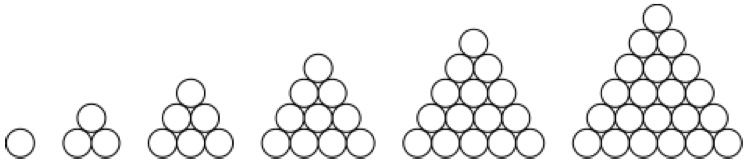
\includegraphics{triangularNumbers}
\end{image}
\fixnote{Maybe start this problem without help.  Need an original graphic.}

\begin{problem}
Blair wanted to find the $551^{st}$ triangular number.  She used a table and looked for a pattern in the \emph{sequence of partial sums}:  $1, 1+2, 1+2+3, \dots$.  Help her finish her idea.  
\end{problem}

\begin{problem}
Kaley realized the the $551^{st}$ triangular number would be the sum 
\[
1+2+3+4+\dots+548+549+550+551
\]
She started pairing the first with the last number; the second with the second-to-last; the third with the third-to-last; and so on.  She saw that the averages are always the same.  Help her finish her idea.  
\end{problem}

\begin{problem}
Ali begin by writing out the sum forward and backward and follows:  
\[
\begin{array}{c@{ + }c@{ + }c@{ + }c@{ + }c@{ + }c@{ + }c@{ + }c@{ + }c@{ + }c@{ + }c@{ + }c@{ + }c}
1 & 2 & 3 & 4 & 5 & 6 & \cdots & 546 & 547 & 548 & 549 & 550 & 551 \\
551 & 550 & 549 & 548 & 547 & 546 & \cdots & 6 & 5 & 4 & 3 & 2 & 1 
\end{array}
\]
Help her finish her idea.  Be sure to explain clearly what happens ``in the dots.''  Does it matter whether there are an even or an odd number of terms?  
\end{problem}

\begin{problem}
Cooper was interested in a different triangular number and drew the following picture:   
\begin{image}
\includegraphics{sum1.pdf}
\end{image}
Which triangular number was he finding?  Help him finish his idea.  Be sure to explain clearly what 
happens ``in the dots.'' 
\end{problem}


\begin{problem}
Sum the numbers:  
\[
106 + 112 + 118 + \dots + 514
\]
\end{problem}

\begin{problem}
Sum the numbers:
\[
2.2 + 2.9 + 3.6 + 4.3 + \dots + 81.3
\]
\end{problem}


\begin{problem}
Suppose you have an arithmetic sequence beginning with $a$, with a constant difference of $d$ and with $n$ terms.  
\begin{enumerate}
\item What is the $n^{th}$ term of the sequence?  
\item Use dots to write the series consisting of the first $n$ terms of this sequence.
\item Find the sum of this series.  
\end{enumerate}
\end{problem}

\end{document}

\newpage
\section{Geometric Series}\label{A:geometicSeries}

In this activity, we explore \emph{geometric series}, which are sums of consecutive terms from an geometric sequence.

Ms. Radigan's math class has been trying to compute the following sums:  
$$1+2+4+8+\dots+2^{19}$$
$$\frac{2}{3}+\frac{2}{9}+\frac{2}{27}+\dots+\frac{2}{3^{13}}$$

\begin{prob}
Kelsey used tables and looked for pattern in the \emph{sequence of partial sums}:  $1, 1+2, 1+2+4, \dots$.  Help her finish her idea for both sequences.    
\end{prob}

\begin{prob}
For the sum beginning with $\frac{2}{3}$, Erin started by drawing a large square (which she imagined as having area 1), and she shaded in $\frac{2}{3}$ of it.  Then she shaded in $\frac{2}{9}$ more, and so on.  Help her finish her idea.  
\end{prob}

\begin{prob}
Ryan wrote out all of the terms in the first sum, represented as powers of 2, beginning with $1+2+2^2+2^3$.  
Then he realized that because the terms formed a geometric sequence, he could multiply the series by the common ratio of 2, and the resulting series would be almost identical to the first, differing only at the beginning and the end.  By subtracting the first series from the second, all of the middle terms would cancel.  Help him finish his idea.  
\end{prob}

\begin{prob}
Ali said, ``Here is a thought experiment.  I take a sheet of paper, rip it perfectly into thirds, place one piece to start a pile that I will call A, another piece to start a pile I will call B, and I keep the third piece in my hands.  I then rip that piece into thirds, place one piece on pile A, one piece on pile B, and keep the third.  Notice that each of pile A and pile B have $\frac{1}{3}+\frac{1}{9}$ of a sheet of paper, and I still have $\frac{1}{9}$ of a sheet in my hands.  I continue this process until I place $\frac{1}{3^{13}}$ of a sheet on each pile and still have $\frac{1}{3^{13}}$ of a sheet in my hands.  

Help Ali finish her idea.  
\end{prob}


\begin{prob}
Sum the expression:  
\[
\frac{2}{3}+\frac{4}{9}+\frac{8}{27}+\dots+\frac{2^n}{3^n}
\]
What happens to this sum as $n$ gets really large?  
\end{prob}


\begin{prob}
Consider the expression: 
$$\frac{7}{10}+\frac{7}{100}+\frac{7}{1000}+\dots+\frac{7}{10^n}$$
\begin{enumerate}
\item Find the sum of the expression. 
\item What happens to this sum as $n$ gets really large?  
\item How does this help you explain why a particular repeating decimal is a particular rational number?  Be sure to indicate what repeating decimal and what rational number you are talking about.  
\end{enumerate}
\end{prob}


\begin{prob}
Suppose you have an geometric sequence beginning with $a$, with a constant ratio of $r$ and with $n$ terms.  
\begin{enumerate}
\item What is the $n^{th}$ term of the sequence?  
\item Use dots to write the series consisting of the first $n$ terms of this sequence.
\item Find the sum of this series.  
\end{enumerate}
\end{prob}



%\documentclass[handout]{ximera}
\documentclass{ximera}

\usepackage{gensymb}
\usepackage{tabularx}
\usepackage{mdframed}
\usepackage{pdfpages}
%\usepackage{chngcntr}

\let\problem\relax
\let\endproblem\relax

\newcommand{\property}[2]{#1#2}




\newtheoremstyle{SlantTheorem}{\topsep}{\fill}%%% space between body and thm
 {\slshape}                      %%% Thm body font
 {}                              %%% Indent amount (empty = no indent)
 {\bfseries\sffamily}            %%% Thm head font
 {}                              %%% Punctuation after thm head
 {3ex}                           %%% Space after thm head
 {\thmname{#1}\thmnumber{ #2}\thmnote{ \bfseries(#3)}} %%% Thm head spec
\theoremstyle{SlantTheorem}
\newtheorem{problem}{Problem}[]

%\counterwithin*{problem}{section}



%%%%%%%%%%%%%%%%%%%%%%%%%%%%Jenny's code%%%%%%%%%%%%%%%%%%%%

%%% Solution environment
%\newenvironment{solution}{
%\ifhandout\setbox0\vbox\bgroup\else
%\begin{trivlist}\item[\hskip \labelsep\small\itshape\bfseries Solution\hspace{2ex}]
%\par\noindent\upshape\small
%\fi}
%{\ifhandout\egroup\else
%\end{trivlist}
%\fi}
%
%
%%% instructorIntro environment
%\ifhandout
%\newenvironment{instructorIntro}[1][false]%
%{%
%\def\givenatend{\boolean{#1}}\ifthenelse{\boolean{#1}}{\begin{trivlist}\item}{\setbox0\vbox\bgroup}{}
%}
%{%
%\ifthenelse{\givenatend}{\end{trivlist}}{\egroup}{}
%}
%\else
%\newenvironment{instructorIntro}[1][false]%
%{%
%  \ifthenelse{\boolean{#1}}{\begin{trivlist}\item[\hskip \labelsep\bfseries Instructor Notes:\hspace{2ex}]}
%{\begin{trivlist}\item[\hskip \labelsep\bfseries Instructor Notes:\hspace{2ex}]}
%{}
%}
%% %% line at the bottom} 
%{\end{trivlist}\par\addvspace{.5ex}\nobreak\noindent\hung} 
%\fi
%
%


\let\instructorNotes\relax
\let\endinstructorNotes\relax
%%% instructorNotes environment
\ifhandout
\newenvironment{instructorNotes}[1][false]%
{%
\def\givenatend{\boolean{#1}}\ifthenelse{\boolean{#1}}{\begin{trivlist}\item}{\setbox0\vbox\bgroup}{}
}
{%
\ifthenelse{\givenatend}{\end{trivlist}}{\egroup}{}
}
\else
\newenvironment{instructorNotes}[1][false]%
{%
  \ifthenelse{\boolean{#1}}{\begin{trivlist}\item[\hskip \labelsep\bfseries {\Large Instructor Notes: \\} \hspace{\textwidth} ]}
{\begin{trivlist}\item[\hskip \labelsep\bfseries {\Large Instructor Notes: \\} \hspace{\textwidth} ]}
{}
}
{\end{trivlist}}
\fi


%% Suggested Timing
\newcommand{\timing}[1]{{\bf Suggested Timing: \hspace{2ex}} #1}




\hypersetup{
    colorlinks=true,       % false: boxed links; true: colored links
    linkcolor=blue,          % color of internal links (change box color with linkbordercolor)
    citecolor=green,        % color of links to bibliography
    filecolor=magenta,      % color of file links
    urlcolor=cyan           % color of external links
}

\title{Second Differences}
\author{Bart Snapp and Brad Findell}

\outcome{Learning outcome goes here.}

\begin{document}
\begin{abstract}
Abstract goes here.  
\end{abstract}
\maketitle

\label{A:secondDifferences}
In a previous activity, we developed strategies for finding the sum of arithmetic series.  In this activity, we use arithmetic series to develop a formula for a sequence that has constant second differences.  Then we demonstrate that all quadratic sequences have constant second differences.  

\begin{problem}
Consider the sequence $f(n)$ given in the table below.  In the rightmost column, $\Delta$ (``delta'') means difference, computed by subtracting the current value of $f(n)$ from the next.  
\vspace{0.1in} 
\[{\renewcommand{\arraystretch}{1.6}
\begin{tabular}{|c|c|c|}\hline
$n$ & $f(n)$ & $\Delta$ \\ \hline
   0     &  \cellcolor{lightgray}4  &  \cellcolor{lightgray}3  \\ \hline
   1     &  7 &   \cellcolor{lightgray}3 \\ \hline
   2     &  10 &  \cellcolor{lightgray}3  \\ \hline
   3     &  13 &  \cellcolor{lightgray}3  \\ \hline
   4     &  16 &  \cellcolor{lightgray}3   \\ \hline
   5     &  19 &    \\ \hline
\rule[5mm]{12mm}{0mm}  &  \rule[5mm]{12mm}{0mm} &\rule[5mm]{12mm}{0mm}    \\ \hline
\end{tabular}}
\]
\vspace{0.1in} 
\begin{enumerate}
\item Explain how $f(5)$ can be computed from the shaded cells in the table.  
\item Generalize your method to develop and explain a formula for $f(n)$.  
\item What was it about the differences that made this problem easy?  
\end{enumerate}
\end{problem}

\newpage

\begin{problem}
Consider the sequence $g(n)$ given in the table below.  
\vspace{0.1in} 
\[{\renewcommand{\arraystretch}{1.6}
\begin{tabular}{|c|c|c|c|}\hline
$n$ & $g(n)$ & $\Delta$ & $\Delta\Delta$ \\ \hline
   0     &  \cellcolor{lightgray}1  &  \cellcolor{lightgray}  & \\ \hline
   1     &  $-2$ &  \cellcolor{lightgray} & \\ \hline
   2     &  1 &  \cellcolor{lightgray}  & \\ \hline
   3     &  10 &  \cellcolor{lightgray} &  \\ \hline
   4     &  25 & \cellcolor{lightgray}  &  \\ \hline
   5     &  46 &   &  \\ \hline
   6     &  73 &   &  \\ \hline
\rule[5mm]{12mm}{0mm}  &  \rule[5mm]{12mm}{0mm} &\rule[5mm]{12mm}{0mm}  &\rule[5mm]{12mm}{0mm}   \\ \hline
\end{tabular}}
\]
\vspace{0.1in} 
\begin{enumerate}
\item Compute $\Delta$ by subtracting the current value of $g(n)$ from the next.  
\item Explain the formula $\Delta(n) = g(n+1)-g(n)$.
\item Check that the shaded cells sum to $g(5)$, and explain how that makes sense based upon how the $\Delta$ values were calculated.  \item Because the $\Delta$ values (``first differences'') are not constant, use the $\Delta\Delta$ column to compute the ``differences of the differences'' (also called ``second differences'').  
\item From the fact that the second differences are constant, develop an explicit formula for $\Delta$ in terms of $n$.  
\end{enumerate}
\end{problem}

\newpage

\begin{problem}
The same sequence $g(n)$ is given below, this time with a formula for $\Delta$ in terms of $n$.    
\vspace{0.1in} 
\[{\renewcommand{\arraystretch}{1.6}
\begin{tabular}{|c|c|c|}\hline
$n$ & $g(n)$ & $\Delta(n)=6n-3$  \\ \hline
   0     &   \cellcolor{lightgray}1  &   \cellcolor{lightgray}$-3$  \\ \hline
   1     &  $-2$ &  \cellcolor{lightgray}3   \\ \hline
   2     &  1 &    \cellcolor{lightgray}9  \\ \hline
   3     &  10 &  \cellcolor{lightgray}15    \\ \hline
   4     &  25 &   \cellcolor{lightgray}21   \\ \hline
   5     &  46 &  27   \\ \hline
   6     &  73 &     \\ \hline
\rule[5mm]{12mm}{0mm}  &  \rule[5mm]{12mm}{0mm} &\rule[5mm]{12mm}{0mm}    \\ \hline
\end{tabular}}
\]
\vspace{0.1in} 
\begin{enumerate}
\item Explain each of the following steps:    
\begin{align*}
g(5) &= 1 + \Delta(0) + \Delta(1) + \Delta(2) + \Delta(3) + \Delta(4)  \\
        &= 1 + (6\cdot 0 -3) + (6\cdot1 -3) + (6\cdot2 -3) + (6\cdot3 -3) + (6\cdot4 -3) \\
        & = 1 + 6\cdot( 0 + 1 + 2 + 3 + 4) + (-3 + -3 + -3 + -3 + -3) \\
        & = 1 + 6\cdot\frac{5\cdot 4}{2} + 5\cdot (-3)
\end{align*}
\item Where do you see arithmetic series in the calculations you just explained?  
\item Generalize the above approach to yield an expression for $g(n)$.  
\item What kind of sequence is $g(n)$?  
\end{enumerate}

\end{problem}

\newpage

\begin{problem}
A general quadratic sequence $h(n)$ is given below.    
\vspace{0.1in} 
\[{\renewcommand{\arraystretch}{1.6}
\begin{tabular}{|c|c|c|c|}\hline
$n$ & $h(n)=an^2+bn+c$ & $\Delta$ & $\Delta\Delta$ \\ \hline
   0     &    &    & \\ \hline
   1     &   &   & \\ \hline
   2     &   &    & \\ \hline
   3     &   &   &  \\ \hline
\rule[5mm]{12mm}{0mm}  &  \rule[5mm]{12mm}{0mm} &\rule[5mm]{30mm}{0mm}  &\rule[5mm]{30mm}{0mm}   \\ \hline
\end{tabular}}
\]
\vspace{0.1in} 
\begin{enumerate}
\item Compute the values of $h(n)$.  
\item Compute $\Delta$ by subtracting the next value of $h(n)$ from the current.  
\item Use the $\Delta\Delta$ column to compute the second differences.  
\item Generalize the result for first differences by computing $\Delta(n)=h(n+1)-h(n)$.
\item Generalize the result for second differences by computing $\Delta\Delta(n)=\Delta(n+1)-\Delta(n)$.
\item Explain how your work demonstrates that, for any quadratic sequence, the second differences must be constant.  
\end{enumerate}
\end{problem}

\end{document}
 % Needs \RequirePackage{xcolor,colortbl}, 
% but then some of the Euclidean Algorithm sections won't compile.  
%\documentclass[handout]{ximera}
\documentclass[nooutcomes]{ximera}

\usepackage{gensymb}
\usepackage{tabularx}
\usepackage{mdframed}
\usepackage{pdfpages}
%\usepackage{chngcntr}

\let\problem\relax
\let\endproblem\relax

\newcommand{\property}[2]{#1#2}




\newtheoremstyle{SlantTheorem}{\topsep}{\fill}%%% space between body and thm
 {\slshape}                      %%% Thm body font
 {}                              %%% Indent amount (empty = no indent)
 {\bfseries\sffamily}            %%% Thm head font
 {}                              %%% Punctuation after thm head
 {3ex}                           %%% Space after thm head
 {\thmname{#1}\thmnumber{ #2}\thmnote{ \bfseries(#3)}} %%% Thm head spec
\theoremstyle{SlantTheorem}
\newtheorem{problem}{Problem}[]

%\counterwithin*{problem}{section}



%%%%%%%%%%%%%%%%%%%%%%%%%%%%Jenny's code%%%%%%%%%%%%%%%%%%%%

%%% Solution environment
%\newenvironment{solution}{
%\ifhandout\setbox0\vbox\bgroup\else
%\begin{trivlist}\item[\hskip \labelsep\small\itshape\bfseries Solution\hspace{2ex}]
%\par\noindent\upshape\small
%\fi}
%{\ifhandout\egroup\else
%\end{trivlist}
%\fi}
%
%
%%% instructorIntro environment
%\ifhandout
%\newenvironment{instructorIntro}[1][false]%
%{%
%\def\givenatend{\boolean{#1}}\ifthenelse{\boolean{#1}}{\begin{trivlist}\item}{\setbox0\vbox\bgroup}{}
%}
%{%
%\ifthenelse{\givenatend}{\end{trivlist}}{\egroup}{}
%}
%\else
%\newenvironment{instructorIntro}[1][false]%
%{%
%  \ifthenelse{\boolean{#1}}{\begin{trivlist}\item[\hskip \labelsep\bfseries Instructor Notes:\hspace{2ex}]}
%{\begin{trivlist}\item[\hskip \labelsep\bfseries Instructor Notes:\hspace{2ex}]}
%{}
%}
%% %% line at the bottom} 
%{\end{trivlist}\par\addvspace{.5ex}\nobreak\noindent\hung} 
%\fi
%
%


\let\instructorNotes\relax
\let\endinstructorNotes\relax
%%% instructorNotes environment
\ifhandout
\newenvironment{instructorNotes}[1][false]%
{%
\def\givenatend{\boolean{#1}}\ifthenelse{\boolean{#1}}{\begin{trivlist}\item}{\setbox0\vbox\bgroup}{}
}
{%
\ifthenelse{\givenatend}{\end{trivlist}}{\egroup}{}
}
\else
\newenvironment{instructorNotes}[1][false]%
{%
  \ifthenelse{\boolean{#1}}{\begin{trivlist}\item[\hskip \labelsep\bfseries {\Large Instructor Notes: \\} \hspace{\textwidth} ]}
{\begin{trivlist}\item[\hskip \labelsep\bfseries {\Large Instructor Notes: \\} \hspace{\textwidth} ]}
{}
}
{\end{trivlist}}
\fi


%% Suggested Timing
\newcommand{\timing}[1]{{\bf Suggested Timing: \hspace{2ex}} #1}




\hypersetup{
    colorlinks=true,       % false: boxed links; true: colored links
    linkcolor=blue,          % color of internal links (change box color with linkbordercolor)
    citecolor=green,        % color of links to bibliography
    filecolor=magenta,      % color of file links
    urlcolor=cyan           % color of external links
}

\title{Hieroglyphical Algebra}
\author{Bart Snapp and Brad Findell}

\outcome{Learning outcome goes here.}

\begin{document}
\begin{abstract}
  We use a strange multiplication table to solve algebra problems.
\end{abstract}
\maketitle

\label{A:HAlgebra} 
Note: This activity is based on an activity originally designed by Lee Wayand.



Consider the following addition and multiplication tables:
%% \[
%% {\renewcommand{\arraystretch}{1.8}
%% \begin{array}{clc}
%% {\renewcommand{\arraystretch}{1.8}
%% \begin{array}{|c||c|c|c|c|c|c|c|c|c|}\hline
%%  +  &\loo & \la & \lo & \lb & \lc & \ld & \lf & \lh & \li \\ \hline\hline
%% \loo& \ld & \lh &\loo & \li & \lb & \lo & \la & \lf & \lc \\ \hline
%% \la & \lh & \li & \la & \ld &\loo & \lf & \lb & \lc & \lo \\ \hline
%% \lo &\loo & \la & \lo & \lb & \lc & \ld & \lf & \lh & \li \\ \hline
%% \lb & \li & \ld & \lb & \lh & \la & \lc &\loo & \lo & \lf \\ \hline
%% \lc & \lb &\loo & \lc & \la & \lf & \li & \lo & \ld & \lh \\ \hline
%% \ld & \lo & \lf & \ld & \lc & \li &\loo & \lh & \la & \lb \\ \hline
%% \lf & \la & \lb & \lf &\loo & \lo & \lh & \lc & \li & \ld \\ \hline
%% \lh & \lf & \lc & \lh & \lo & \ld & \la & \li & \lb &\loo \\ \hline
%% \li & \lc & \lo & \li & \lf & \lh & \lb & \ld &\loo & \la \\ \hline
%% \end{array}}
%% \vspace{.5cm}
%% & 
%% \begin{array}{l}
%% \text{$\loo =$ fish} \\ 
%% \text{$\la =$ lolly-pop} \\ 
%% \text{$\lo =$ skull} \\ 
%% \text{$\lb =$ cinder-block} \\ 
%% \text{$\lc =$ DNA} \\ 
%% \text{$\ld =$ fork} \\ 
%% \text{$\lf =$ man} \\ 
%% \text{$\lh =$ balloon} \\ 
%% \text{$\li =$ eyeball} 
%% \end{array}
%% & 
%% {\renewcommand{\arraystretch}{1.8}
%% \begin{array}{|c||c|c|c|c|c|c|c|c|c|}\hline
%% \cdot & \ld & \li & \lh & \lf & \lo & \la & \lb & \lc &\loo \\ \hline\hline
%% \ld   &\loo & \la & \lb & \lc & \lo & \li & \lh & \lf & \ld \\ \hline
%% \li   & \la & \lh & \lf & \ld & \lo & \lb & \lc &\loo & \li \\ \hline
%% \lh   & \lb & \lf & \ld & \la & \lo & \lc &\loo & \li & \lh \\ \hline
%% \lf   & \lc & \ld & \la & \lb & \lo &\loo & \li & \lh & \lf \\ \hline
%% \lo   & \lo & \lo & \lo & \lo & \lo & \lo & \lo & \lo & \lo \\ \hline
%% \la   & \li & \lb & \lc &\loo & \lo & \lh & \lf & \ld & \la \\ \hline
%% \lb   & \lh & \lc &\loo & \li & \lo & \lf & \ld & \la & \lb \\ \hline
%% \lc   & \lf &\loo & \li & \lh & \lo & \ld & \la & \lb & \lc \\ \hline
%% \loo  & \ld & \li & \lh & \lf & \lo & \la & \lb & \lc &\loo \\ \hline
%% \end{array}} 
%% \end{array}}
%% \]
\[
\renewcommand{\arraystretch}{1.8}
\begin{array}{cl}
\begin{array}{|c||c|c|c|c|c|c|c|c|c|}\hline
 +  &\loo & \la & \lo & \lb & \lc & \ld & \lf & \lh & \li \\ \hline\hline
\loo& \ld & \lh &\loo & \li & \lb & \lo & \la & \lf & \lc \\ \hline
\la & \lh & \li & \la & \ld &\loo & \lf & \lb & \lc & \lo \\ \hline
\lo &\loo & \la & \lo & \lb & \lc & \ld & \lf & \lh & \li \\ \hline
\lb & \li & \ld & \lb & \lh & \la & \lc &\loo & \lo & \lf \\ \hline
\lc & \lb &\loo & \lc & \la & \lf & \li & \lo & \ld & \lh \\ \hline
\ld & \lo & \lf & \ld & \lc & \li &\loo & \lh & \la & \lb \\ \hline
\lf & \la & \lb & \lf &\loo & \lo & \lh & \lc & \li & \ld \\ \hline
\lh & \lf & \lc & \lh & \lo & \ld & \la & \li & \lb &\loo \\ \hline
\li & \lc & \lo & \li & \lf & \lh & \lb & \ld &\loo & \la \\ \hline
\end{array}
& 
\begin{array}{l}
\text{$\loo =$ fish} \\ 
\text{$\la =$ lolly-pop} \\ 
\text{$\lo =$ skull} \\ 
\text{$\lb =$ cinder-block} \\ 
\text{$\lc =$ DNA} \\ 
\text{$\ld =$ fork} \\ 
\text{$\lf =$ man} \\ 
\text{$\lh =$ balloon} \\ 
\text{$\li =$ eyeball} 
\end{array}
\end{array}
\]



\[
\renewcommand{\arraystretch}{1.8}
\begin{array}{cl}
\begin{array}{|c||c|c|c|c|c|c|c|c|c|}\hline
\cdot & \ld & \li & \lh & \lf & \lo & \la & \lb & \lc &\loo \\ \hline\hline
\ld   &\loo & \la & \lb & \lc & \lo & \li & \lh & \lf & \ld \\ \hline
\li   & \la & \lh & \lf & \ld & \lo & \lb & \lc &\loo & \li \\ \hline
\lh   & \lb & \lf & \ld & \la & \lo & \lc &\loo & \li & \lh \\ \hline
\lf   & \lc & \ld & \la & \lb & \lo &\loo & \li & \lh & \lf \\ \hline
\lo   & \lo & \lo & \lo & \lo & \lo & \lo & \lo & \lo & \lo \\ \hline
\la   & \li & \lb & \lc &\loo & \lo & \lh & \lf & \ld & \la \\ \hline
\lb   & \lh & \lc &\loo & \li & \lo & \lf & \ld & \la & \lb \\ \hline
\lc   & \lf &\loo & \li & \lh & \lo & \ld & \la & \lb & \lc \\ \hline
\loo  & \ld & \li & \lh & \lf & \lo & \la & \lb & \lc &\loo \\ \hline
\end{array}
& 
\begin{array}{l}
\text{$\loo =$ fish} \\ 
\text{$\la =$ lolly-pop} \\ 
\text{$\lo =$ skull} \\ 
\text{$\lb =$ cinder-block} \\ 
\text{$\lc =$ DNA} \\ 
\text{$\ld =$ fork} \\ 
\text{$\lf =$ man} \\ 
\text{$\lh =$ balloon} \\ 
\text{$\li =$ eyeball} 
\end{array}
\end{array}
\]
\newpage



\begin{problem} 
Can you tell me which glyph represents $0$? How did you arrive at this
conclusion?
\end{problem}

\begin{problem} 
Can you tell me which glyph represents $1$? How did you arrive at this
conclusion?
\end{problem}

\begin{problem}
A number $x$ has an \textit{additive inverse} if you can find another number $y$ with 
\[
x + y = 0.
\]
and we say that ``$y$ is the additive inverse for $x$.'' If possible,
find the additive inverse of every number in the table above.
\end{problem}

\begin{problem}
A number $x$ has a \textit{multiplicative inverse} if you can find
another number $y$ with
\[
x\cdot y = 1.
\]
and we say that ``$y$ is the multiplicative inverse for $x$.'' If
possible, find the multiplicative inverse of every number in the
table above.
\end{problem}



\begin{problem} If possible, solve the following equations:
\begin{enumerate}
\item $\lh \cdot \lx - \lb = \ld$
\item $\dfrac{\ly}{\lb} = \dfrac{\ld}{\loo}$
\item $\bigg(\lz - \ld\bigg)\bigg(\lz + \lf\bigg)=\loo$
\item $\dfrac{\loo - \lw}{\lc} + \ld = \dfrac{\lh}{\lf}$
\end{enumerate}
In each case explain your reasoning.
\end{problem}

\begin{problem} If possible, solve the following equations:
\begin{enumerate}
\item $\lx \cdot \lx = \ld$
\item $\lz\cdot \lz = \lf$
\item $\ly\cdot \ly + \ly \cdot \lb = \loo$
\item $\lw \cdot \lw+ \lc = \lw$
\end{enumerate}
In each case explain your reasoning.
\end{problem}

\end{document}

\newpage
\section{The Other Side---Solving Equations}\label{A:otherSide}


In this activity, we will explore ideas related to solving equations.


\begin{prob}
Solve the following equation three ways: Using algebra, using the
balance, and with the graph. At each step, the three models should be in
complete alignment.
\[
\]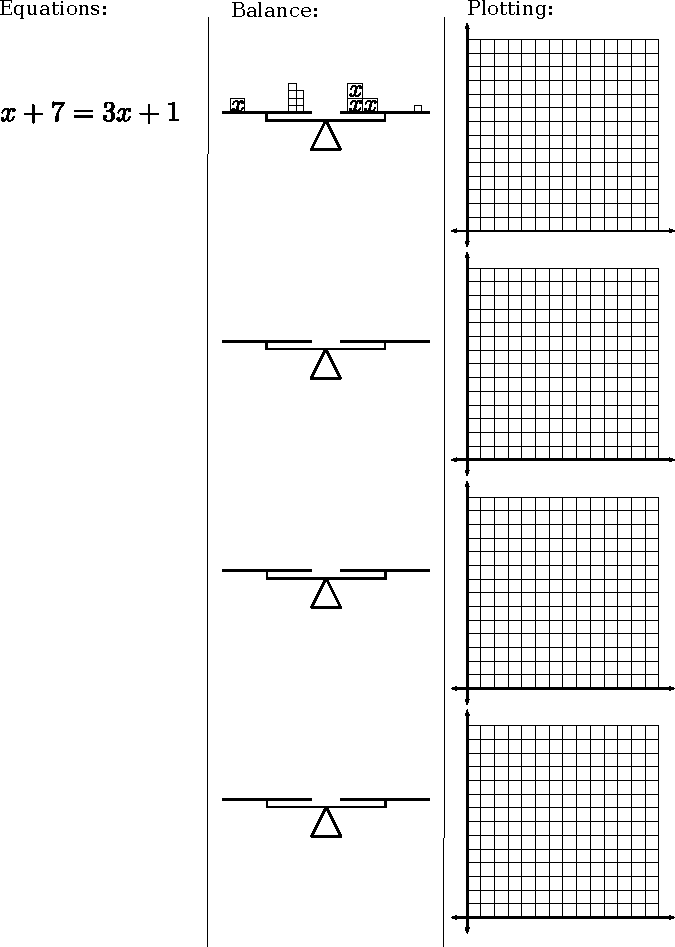
\includegraphics[scale=0.8]{../graphics/eqBalGraph.pdf}
\end{prob}


\begin{prob}
Critically analyze the three ``different'' methods of solving
equations, noting the advantages and disadvantages of each. 
\end{prob}

\begin{prob}
Can you solve quadratic equations using the methods above?
If so give an example. If not, explain why not.
\end{prob}

\begin{teachingnote}
The key point here is that it is difficult to make ``balances'' work for anything but linear equations.  But the graphical approach always works, as described in the following standard:  

CCSS.A-REI.11.  Explain why the $x$-coordinates of the points where the graphs of the equations $y = f(x)$ and $y = g(x)$ intersect are the solutions of the equation $f(x) = g(x)$; find the solutions approximately, e.g., using technology to graph the functions, make tables of values, or find successive approximations. Include cases where $f(x)$ and/or $g(x)$ are linear, polynomial, rational, absolute value, exponential, and logarithmic functions.*
\end{teachingnote}


\begin{prob}
Can you think of an example when the undoing via algebraic
manipulation would fail?
\end{prob}

\begin{teachingnote}
Here we are looking for something where an inverse function must be
applied, as in $.6 = \sin(x)$.
\end{teachingnote}


While sometimes we solve equations via a process of algebraic
manipulation, other times we have a formula.


\begin{prob}
Give a formula for solving linear equations of the form $ax + b =0$.
\end{prob}





\newpage
\section{Solving Quadratics}\label{A:solvingQuadratics}
Here we explore various methods for solving quadratic equations in one variable.  \textbf{Please read all instructions carefully.}

\begin{prob}
Is $\sqrt{4}=\pm 2$?  Explain. 
\end{prob}

\vfill

\begin{teachingnote}
Both $2$ and $-2$ are ``square roots'' of $4$ because $2^2=4$ and $(-2)^2=4$, and both of them are solutions to the equation $x^2=4$.  The question is whether the radical symbol refers to both of them, either of them (you choose?), or a specific one of them.  
\end{teachingnote}

\begin{prob}
Suppose that $\sqrt{4}=\pm 2$?  Then evaluate $\sqrt{4}+\sqrt{9}$.  
\end{prob}

\begin{teachingnote}
$$\sqrt{4}+\sqrt{9}=\pm2+\pm3=5, -1, 1, or -5$$
\end{teachingnote}

\vfill

\begin{prob}
What does your calculator say about $\sqrt{4}+\sqrt{9}$?  
\end{prob}

\vfill 

\begin{teachingnote}
Now emphasize the conventional meaning of the radical symbol:  For $a>0$ then $\sqrt{a}$ means the positive square root of $a$.  
\end{teachingnote}



\begin{prob}
In the following problems, you \textbf{may not use the quadratic formula}.  But just for the record, write down the quadratic formula.  
\end{prob}
\begin{teachingnote}
Many students will write only $\frac{-b\pm\sqrt{b^2-4ac}}{2a}$, but we want them to write the following:  
$$\text{If }ax^2+bx+c=0\text{ and }a\ne 0\text{, then }x=\frac{-b\pm\sqrt{b^2-4ac}}{2a}\text{.}$$
Note that if the radical symbol were to refer to both a positive and negative square root, then there would be no reason to write $\pm$ outside the radical symbol.  
\end{teachingnote}
\vspace{0.8in}

\begin{prob}
In the following list of equations, solve those that are \textbf{easy} to solve.  
\begin{enumerate}
\item $(x-3)(x+2)=0$
\item $(x-3)(x+2)=1$
\item $(2x-5)(3x+1)=0$
\item $(x-a)(x-b)=0$
\item $(x-1)(x-3)(x+2)(2x-3)=0$
\end{enumerate}
\end{prob}

\begin{prob}
Regarding the previous problem, state the property of numbers that made all but one of the equations easy to solve.  
\end{prob}

\begin{teachingnote}
Zero product property:  If $ab = 0$ then $a=0$ or $b=0$.  Note that this doesn't work when the right side is not 0.  
\end{teachingnote}

\vspace{0.3in}


%\begin{prob} For each part below, write a linear equation with the state solution.  
%\begin{enumerate}
%\item $x=\frac{2}{3}$
%\item $x=\frac{a}{b}$
%\end{enumerate}
%\end{prob}

\begin{prob}For each part below, write a quadratic equation with the stated solution(s) and no other solutions.  
\begin{enumerate}
\item $x=7$ or $x=-4$
\item $x=p$ or $x=q$
\item $x=3$
\item $x=\frac{1\pm\sqrt{5}}{2}$
 \end{enumerate}
\end{prob}

\begin{prob}
Find all solutions to $x^3-3x^2+x+1=0$.  Hint:  One solution is $x=1$.  
\end{prob}

%\documentclass[handout]{ximera}
\documentclass{ximera}

\usepackage{gensymb}
\usepackage{tabularx}
\usepackage{mdframed}
\usepackage{pdfpages}
%\usepackage{chngcntr}

\let\problem\relax
\let\endproblem\relax

\newcommand{\property}[2]{#1#2}




\newtheoremstyle{SlantTheorem}{\topsep}{\fill}%%% space between body and thm
 {\slshape}                      %%% Thm body font
 {}                              %%% Indent amount (empty = no indent)
 {\bfseries\sffamily}            %%% Thm head font
 {}                              %%% Punctuation after thm head
 {3ex}                           %%% Space after thm head
 {\thmname{#1}\thmnumber{ #2}\thmnote{ \bfseries(#3)}} %%% Thm head spec
\theoremstyle{SlantTheorem}
\newtheorem{problem}{Problem}[]

%\counterwithin*{problem}{section}



%%%%%%%%%%%%%%%%%%%%%%%%%%%%Jenny's code%%%%%%%%%%%%%%%%%%%%

%%% Solution environment
%\newenvironment{solution}{
%\ifhandout\setbox0\vbox\bgroup\else
%\begin{trivlist}\item[\hskip \labelsep\small\itshape\bfseries Solution\hspace{2ex}]
%\par\noindent\upshape\small
%\fi}
%{\ifhandout\egroup\else
%\end{trivlist}
%\fi}
%
%
%%% instructorIntro environment
%\ifhandout
%\newenvironment{instructorIntro}[1][false]%
%{%
%\def\givenatend{\boolean{#1}}\ifthenelse{\boolean{#1}}{\begin{trivlist}\item}{\setbox0\vbox\bgroup}{}
%}
%{%
%\ifthenelse{\givenatend}{\end{trivlist}}{\egroup}{}
%}
%\else
%\newenvironment{instructorIntro}[1][false]%
%{%
%  \ifthenelse{\boolean{#1}}{\begin{trivlist}\item[\hskip \labelsep\bfseries Instructor Notes:\hspace{2ex}]}
%{\begin{trivlist}\item[\hskip \labelsep\bfseries Instructor Notes:\hspace{2ex}]}
%{}
%}
%% %% line at the bottom} 
%{\end{trivlist}\par\addvspace{.5ex}\nobreak\noindent\hung} 
%\fi
%
%


\let\instructorNotes\relax
\let\endinstructorNotes\relax
%%% instructorNotes environment
\ifhandout
\newenvironment{instructorNotes}[1][false]%
{%
\def\givenatend{\boolean{#1}}\ifthenelse{\boolean{#1}}{\begin{trivlist}\item}{\setbox0\vbox\bgroup}{}
}
{%
\ifthenelse{\givenatend}{\end{trivlist}}{\egroup}{}
}
\else
\newenvironment{instructorNotes}[1][false]%
{%
  \ifthenelse{\boolean{#1}}{\begin{trivlist}\item[\hskip \labelsep\bfseries {\Large Instructor Notes: \\} \hspace{\textwidth} ]}
{\begin{trivlist}\item[\hskip \labelsep\bfseries {\Large Instructor Notes: \\} \hspace{\textwidth} ]}
{}
}
{\end{trivlist}}
\fi


%% Suggested Timing
\newcommand{\timing}[1]{{\bf Suggested Timing: \hspace{2ex}} #1}




\hypersetup{
    colorlinks=true,       % false: boxed links; true: colored links
    linkcolor=blue,          % color of internal links (change box color with linkbordercolor)
    citecolor=green,        % color of links to bibliography
    filecolor=magenta,      % color of file links
    urlcolor=cyan           % color of external links
}

\title{Complete Squares}
\author{Bart Snapp and Brad Findell}

\outcome{Learning outcome goes here.}

\begin{document}
\begin{abstract}
Abstract goes here.  
\end{abstract}
\maketitle

\label{A:completeSquares}

\begin{problem}
In the following list of equations, solve those that are \textbf{easy} to solve.  
\begin{enumerate}
\item $x^2=5$
\item $x^2 - 4 = 2$
\item $x^2 - 4x = 2$
\item $2x^2=1$
\item $(x-2)^2=5$
\end{enumerate}
\end{problem}
\vspace{0.3in}

\begin{problem}
Regarding the previous problem, state the property of numbers that made all but one of the equations easy to solve.  
\begin{teachingnote}
If $u^2=a$ then $u=\pm\sqrt{a}$.  Be sure to spend some time discussing why 
$$\pm\sqrt{\frac{1}{2}}=\pm\frac{1}{\sqrt{2}}=\pm\frac{\sqrt{2}}{2}.$$
\end{teachingnote}
\vspace{0.3in}
\end{problem}

\begin{problem}
Although $160$ is not a square in base ten, what could you add to $160$ so that the result would be a square number?  
\end{problem}

\begin{problem}
 Consider the polynomial expression $x^2+6x$ to be a number in base $x$.  We want to add to this polynomial so that the result is a square in base $x$.  
\begin{enumerate}
\item Use ``flats'' and ``longs'' to draw a picture of this polynomial as a number in base $x$, adding enough ``ones'' so that you can arrange the polynomial into a square.  
\vspace{0.5in}
\item What ``feature'' of the square does the new polynomial expression represent?  
\item Why does it make sense to call this technique ``completing the square''? 
\item Use your picture to help you solve the equation $x^2+6x=5$.  
\end{enumerate}
\end{problem}


\begin{problem}
Complete the square to solve the following equations: 
\begin{enumerate}
\item $x^2+3x=4$
\vspace{.8in}
\item $x^2+bx=q$
\vspace{.8in}
\item $2x^2+8x=12$
\vspace{.8in}
\item $ax^2+bx+c=0$
\vspace{.8in}
\end{enumerate}  
\end{problem}

\begin{problem}
Solve the following equation
\[
x^5 - 4x^4 - 18x^3 + 64x^2 + 17x -60 = 0
\]
assuming you know that $1$, $-1$, and $3$ are roots.
\end{problem}

\end{document}

%\documentclass[handout]{ximera}
\documentclass[nooutcomes]{ximera}

\usepackage{gensymb}
\usepackage{tabularx}
\usepackage{mdframed}
\usepackage{pdfpages}
%\usepackage{chngcntr}

\let\problem\relax
\let\endproblem\relax

\newcommand{\property}[2]{#1#2}




\newtheoremstyle{SlantTheorem}{\topsep}{\fill}%%% space between body and thm
 {\slshape}                      %%% Thm body font
 {}                              %%% Indent amount (empty = no indent)
 {\bfseries\sffamily}            %%% Thm head font
 {}                              %%% Punctuation after thm head
 {3ex}                           %%% Space after thm head
 {\thmname{#1}\thmnumber{ #2}\thmnote{ \bfseries(#3)}} %%% Thm head spec
\theoremstyle{SlantTheorem}
\newtheorem{problem}{Problem}[]

%\counterwithin*{problem}{section}



%%%%%%%%%%%%%%%%%%%%%%%%%%%%Jenny's code%%%%%%%%%%%%%%%%%%%%

%%% Solution environment
%\newenvironment{solution}{
%\ifhandout\setbox0\vbox\bgroup\else
%\begin{trivlist}\item[\hskip \labelsep\small\itshape\bfseries Solution\hspace{2ex}]
%\par\noindent\upshape\small
%\fi}
%{\ifhandout\egroup\else
%\end{trivlist}
%\fi}
%
%
%%% instructorIntro environment
%\ifhandout
%\newenvironment{instructorIntro}[1][false]%
%{%
%\def\givenatend{\boolean{#1}}\ifthenelse{\boolean{#1}}{\begin{trivlist}\item}{\setbox0\vbox\bgroup}{}
%}
%{%
%\ifthenelse{\givenatend}{\end{trivlist}}{\egroup}{}
%}
%\else
%\newenvironment{instructorIntro}[1][false]%
%{%
%  \ifthenelse{\boolean{#1}}{\begin{trivlist}\item[\hskip \labelsep\bfseries Instructor Notes:\hspace{2ex}]}
%{\begin{trivlist}\item[\hskip \labelsep\bfseries Instructor Notes:\hspace{2ex}]}
%{}
%}
%% %% line at the bottom} 
%{\end{trivlist}\par\addvspace{.5ex}\nobreak\noindent\hung} 
%\fi
%
%


\let\instructorNotes\relax
\let\endinstructorNotes\relax
%%% instructorNotes environment
\ifhandout
\newenvironment{instructorNotes}[1][false]%
{%
\def\givenatend{\boolean{#1}}\ifthenelse{\boolean{#1}}{\begin{trivlist}\item}{\setbox0\vbox\bgroup}{}
}
{%
\ifthenelse{\givenatend}{\end{trivlist}}{\egroup}{}
}
\else
\newenvironment{instructorNotes}[1][false]%
{%
  \ifthenelse{\boolean{#1}}{\begin{trivlist}\item[\hskip \labelsep\bfseries {\Large Instructor Notes: \\} \hspace{\textwidth} ]}
{\begin{trivlist}\item[\hskip \labelsep\bfseries {\Large Instructor Notes: \\} \hspace{\textwidth} ]}
{}
}
{\end{trivlist}}
\fi


%% Suggested Timing
\newcommand{\timing}[1]{{\bf Suggested Timing: \hspace{2ex}} #1}




\hypersetup{
    colorlinks=true,       % false: boxed links; true: colored links
    linkcolor=blue,          % color of internal links (change box color with linkbordercolor)
    citecolor=green,        % color of links to bibliography
    filecolor=magenta,      % color of file links
    urlcolor=cyan           % color of external links
}

\title{Maximums and Minimums}
\author{Bart Snapp and Brad Findell}

\outcome{Learning outcome goes here.}

\begin{document}
\begin{abstract}
  We think about different forms of quadratic equations.
\end{abstract}
\maketitle

\label{A:vertex}

%\begin{teachingnote}
%This activity will be necessary for computing least squares approximation.
%\end{teachingnote}

%
%While you might have encountered completing the
%square\index{completing the square} first when solving quadratic
%equations, its real power is in transforming the form of an
%expression to reveal properties of that expression. 
%
%In this activity, we'll see it in action.

  

In high school mathematics, you saw three different forms for quadratic functions.  In this activity, we explore the advantages and disadvantages of each.  

Note:  We use only real numbers for $x$.  And we begin by agreeing that the shape of the graph of a quadratic function is a parabola.  

\begin{problem}
Consider the function $f(x) = x^2 -3$. What are the maximum/minimum value(s) of $f(x)$, and for what $x$ values do they occur? 
Explain your reasoning.  Use this information to sketch a graph.  
\end{problem}

\begin{problem}
Consider the function $f(x) = 3(x-5)^2 +7$. What are the maximum/minimum value(s) of $f(x)$, and for what $x$ values do they occur? Explain your reasoning.  Use this information to sketch a graph.  
\end{problem}

\begin{problem}
Consider the function $f(x) = -2(x+3)^2 + 7$. What are the maximum/minimum value(s) of $f(x)$, and for what $x$ values do they occur? Explain your reasoning.  Use this information to sketch a graph.  
\end{problem}

\begin{problem}
What are the advantages of the form $f(x) = a(x-h)^2+k$ for a quadratic function?  Why is it called vertex form?  What do the values of $a$, $h$, and $k$ tell you about the graph?  
\end{problem}


\begin{problem}
Consider the function $f(x) = x^2 + 4x + 2$. Complete the square to
put this function into vertex form, and sketch a graph.
\end{problem}

\vfill

\begin{problem}
Consider the function $f(x) = 2x^2 - 8x + 6$. Complete the square to
put this function into vertex form, and sketch a graph.
\end{problem}

\vfill
\newpage

\begin{problem}
Consider the function $f(x) = (x+1)(x+5)$.  
\begin{enumerate}
\item What points on the graph are easy to locate?  
\item How can you use those points to find the vertex? 
\item Sketch the graph. 
\end{enumerate}
\end{problem}


\begin{problem}
Consider the function $f(x) = -2(x-2)(x+3)$.  
\begin{enumerate}
\item What points on the graph are easy to locate?  
\item How can you use those points to find the vertex? 
\item Sketch the graph. 
\end{enumerate}
\end{problem}

\begin{problem}
Consider the function $f(x) = a(x-r_1)(x-r_2)$.  
\begin{enumerate}
\item What do the values of $a$, $r_1$, and $r_2$ tell you about the graph?  
\item How can you use that information to find the vertex? 
\item What is this form called and why?  
\end{enumerate}
\end{problem}

\begin{problem}
Consider the function $f(x) = ax^2+bx+c$.  
\begin{enumerate}
\item What do the values of $a$, $b$, and $c$ tell you about the graph?  
\item What are the advantages and disadvantages of this form?  
\end{enumerate}
\end{problem}


%\begin{problem}
%Consider the parabola $f(x) = 3x^2 + 7x - 1$. Complete the square to
%put this expression in the form above and identify the maximum/minimum
%value(s) of this curve.
%\end{problem}
%
%
%\begin{problem}
%Given a parabola $f(x) = ax^2 + bx +c$. Complete the square to put
%this expression in the form above and identify the maximum/minimum
%value(s) of this curve.
%\end{problem}
%
%
%\begin{problem}
%Could you find the same formula found in the previous question by
%appealing to the symmetry of the roots?
%\end{problem}

\end{document}

%\newpage
\section{Least Squares Approximation}\label{A:leastSquares}

In this activity, we are going to investigate \textit{least
squares approximation}\index{least squares approximation}.

\begin{prob}
Consider the following data:
\{(2,3), (4,5), (6,11)\}
\[

\includegraphics{../graphics/complexPlane.pdf}
\]
Plot the data and use a ruler to sketch a ``best fit'' line.
\end{prob}

\begin{prob}
Now we are going to record some more data in the chart below:
\begin{enumerate}
\item  For each data point, use a ruler to measure the vertical distance between the point and the line. Record this in the first empty row of the table below.
\item For each data point, square the vertical distance. Record this in the second empty row of the table below.
\end{enumerate}
\[
{\renewcommand{\arraystretch}{1.8}
\renewcommand{\arraycolsep}{3mm}
\begin{array}{|l||c|c|c|c|}\hline
\text{Point} & (2,3) & (4,5) & (6,11)  \\ \hline\hline
\text{Vertical Distance} & & & \\ \hline
\text{Squares} & & & \\ \hline
\end{array}}
\]
\end{prob}

\begin{prob}
Add up the squares of the vertical distances. You want this to be as
small as possible. Compare your sum with that of a friend, or enemy.
Whoever got the smallest value has the best approximation of the given data.
\end{prob}

\begin{prob}
Now find the equation of the line you drew. Write it down and don't
forget it!
\end{prob}

So far we've just been ``eye-balling'' our data. Let's roll up our
sleaves and do some real math.

\begin{prob}
Suppose that your line is $\l(x) = ax + b$. Give an expression
representing the sum of squares you get with your data above.
\end{prob}

\begin{teachingnote}
Here we're looking for something like:
\[
(a\cdot 2+ b -3)^2 + (a\cdot 4+ b -5)^2 + (a\cdot 6+ b -11)^2
\]
\end{teachingnote}

\begin{prob}
Simplfy the expression above. You should now have a quadratic in two
variables $a$ and $b$. Find the minimum, thinking of this as quadratic equation in $a$ and then thinking of this as a quadratic equation in $b$. 
\end{prob}

\begin{prob}
You should now have two equations, and two unknowns---solve!
\end{prob}


\begin{prob}
Compare your computed formula with the line you guessed---how did you
do?
\end{prob}

%\documentclass[handout]{ximera}
\documentclass{ximera}

\usepackage{gensymb}
\usepackage{tabularx}
\usepackage{mdframed}
\usepackage{pdfpages}
%\usepackage{chngcntr}

\let\problem\relax
\let\endproblem\relax

\newcommand{\property}[2]{#1#2}




\newtheoremstyle{SlantTheorem}{\topsep}{\fill}%%% space between body and thm
 {\slshape}                      %%% Thm body font
 {}                              %%% Indent amount (empty = no indent)
 {\bfseries\sffamily}            %%% Thm head font
 {}                              %%% Punctuation after thm head
 {3ex}                           %%% Space after thm head
 {\thmname{#1}\thmnumber{ #2}\thmnote{ \bfseries(#3)}} %%% Thm head spec
\theoremstyle{SlantTheorem}
\newtheorem{problem}{Problem}[]

%\counterwithin*{problem}{section}



%%%%%%%%%%%%%%%%%%%%%%%%%%%%Jenny's code%%%%%%%%%%%%%%%%%%%%

%%% Solution environment
%\newenvironment{solution}{
%\ifhandout\setbox0\vbox\bgroup\else
%\begin{trivlist}\item[\hskip \labelsep\small\itshape\bfseries Solution\hspace{2ex}]
%\par\noindent\upshape\small
%\fi}
%{\ifhandout\egroup\else
%\end{trivlist}
%\fi}
%
%
%%% instructorIntro environment
%\ifhandout
%\newenvironment{instructorIntro}[1][false]%
%{%
%\def\givenatend{\boolean{#1}}\ifthenelse{\boolean{#1}}{\begin{trivlist}\item}{\setbox0\vbox\bgroup}{}
%}
%{%
%\ifthenelse{\givenatend}{\end{trivlist}}{\egroup}{}
%}
%\else
%\newenvironment{instructorIntro}[1][false]%
%{%
%  \ifthenelse{\boolean{#1}}{\begin{trivlist}\item[\hskip \labelsep\bfseries Instructor Notes:\hspace{2ex}]}
%{\begin{trivlist}\item[\hskip \labelsep\bfseries Instructor Notes:\hspace{2ex}]}
%{}
%}
%% %% line at the bottom} 
%{\end{trivlist}\par\addvspace{.5ex}\nobreak\noindent\hung} 
%\fi
%
%


\let\instructorNotes\relax
\let\endinstructorNotes\relax
%%% instructorNotes environment
\ifhandout
\newenvironment{instructorNotes}[1][false]%
{%
\def\givenatend{\boolean{#1}}\ifthenelse{\boolean{#1}}{\begin{trivlist}\item}{\setbox0\vbox\bgroup}{}
}
{%
\ifthenelse{\givenatend}{\end{trivlist}}{\egroup}{}
}
\else
\newenvironment{instructorNotes}[1][false]%
{%
  \ifthenelse{\boolean{#1}}{\begin{trivlist}\item[\hskip \labelsep\bfseries {\Large Instructor Notes: \\} \hspace{\textwidth} ]}
{\begin{trivlist}\item[\hskip \labelsep\bfseries {\Large Instructor Notes: \\} \hspace{\textwidth} ]}
{}
}
{\end{trivlist}}
\fi


%% Suggested Timing
\newcommand{\timing}[1]{{\bf Suggested Timing: \hspace{2ex}} #1}




\hypersetup{
    colorlinks=true,       % false: boxed links; true: colored links
    linkcolor=blue,          % color of internal links (change box color with linkbordercolor)
    citecolor=green,        % color of links to bibliography
    filecolor=magenta,      % color of file links
    urlcolor=cyan           % color of external links
}

\title{Solving Cubic Equations}
\author{Bart Snapp and Brad Findell}

\outcome{Learning outcome goes here.}

\begin{document}
\begin{abstract}
Abstract goes here.  
\end{abstract}
\maketitle

\label{A:solvingCubics}

To solve the cubic equation $x^3+px+q=0$, we use methods that were discovered and advanced by various mathematicians, including Ferro, Tartaglia, and Cardano.  The approach is organized in three steps.  \textbf{Make notes in the margin as you follow along.}  

%\begin{itemize}
%\item Step 1:  Replace $x$ with $u+v$.
%\item Step 2: Set $uv$ so that all of the terms are eliminated except for $u^3$, $v^3$, and constant terms.
%\item Step 3: Clear denominators, recognize the equation as a quadratic in $u^3$, and use the quadratic formula.
%\end{itemize}

\subsection{Step 1:  Replace $x$ with $u+v$}
In $x^3+px+q=0$, let $x = u + v$.  % $$(u+v)^3+p(u+v)+q=0.$$ 
Show that the result can be written as follows:  

$$u^3+v^3+(3uv+p)(u+v)+q = 0.$$

\subsection{Step 2: Set $uv$ to eliminate terms}
If $3uv+p=0$, then all of the terms are eliminated except for $u^3$, $v^3$, and constant terms. Explain why the equation simplifies nicely to:

$$u^3+v^3 + q = 0.$$

Solve $3uv+p=0$ for $v$, substitute, and show that we have:  

$$u^3+\left( \frac{-p}{3u}\right)^3+q=0.$$

\subsection{Step 3:  Recognize the equation as a quadratic in $u^3$ and solve}

By multiplying by $u^3$, show that we get a quadratic in $u^3$:   

$$u^6+qu^3+\left( \frac{-p}{3}\right)^3 = 0.$$

Show that this has solutions: 

$$u^3 = \frac{-q\pm\sqrt{q^2-4\left( \frac{-p}{3}\right)^3}}{2}.$$

Now, use the facts $v= -p/(3u)$ and $x = u + v$ to write a formula for $x$: 

$$x = \sqrt[3]{\frac{-q\pm\sqrt{q^2-4\left( \frac{-p}{3}\right)^3}}{2}} 
+  \frac{-p}{3\sqrt[3]{\frac{-q\pm\sqrt{q^2-4\left( \frac{-p}{3}\right)^3}}{2}}}.$$

\begin{problem}
How many values does this formula give for $x$?  From the original equation $x^3+px+q=0$, how many solutions should we expect? 
\end{problem}
\vfill

\begin{problem}
Use the above formula to solve the specific equation $x^3-15x-4=0$.  Show that $$x = \sqrt[3]{2 \pm \sqrt{-121}} + \frac{5}{\sqrt[3]{2\pm\sqrt{-121}}}.$$
Are these values of $x$ real numbers?  
\end{problem}
\vfill


\begin{problem}
Use technology to graph $y=x^3-15x-4$.  According to the graph, how many real roots does the polynomial have?  What is going on?  
\end{problem}
\vfill

\begin{problem}
Choose ``plus'' in the $\pm$, and check that $2+\sqrt{-1}$ is a cube root of $2 + \sqrt{-121}$.  Use that fact to simplify the above expression for $x$.  What do you notice?  
\end{problem}
\vfill

\begin{problem}
Now choose ``minus'' in the $\pm$ above, and find the value of $x$.  What do you notice?  
\end{problem}

\vfill
In both cases, the formula requires computations with square roots of negative numbers, but the result is a real solution.  These kinds of occurrences were the historical impetus behind the gradual acceptance of complex numbers.  

\end{document}

%\newpage
\section{It Takes All Kinds\dots}\label{A:otherCurves}
\fixnote{Maybe move these to problems.  Replace with linear, quadratic, exponential sheet.}

Data can come in all shapes and sizes. While a line is the simplest
approximation, it might not be the best.

\begin{prob}
Consider the data below:
\[
\begin{array}{|c|c|c|c|c|}\hline
x & 0 & 1 & 2 & 3 \\ \hline
y & 8.1 & 22.1 & 60.1 & 165 \\ \hline
\end{array}
\]
What type of data is this? To get the ``brain
juices'' flowing here are some choices. It could be:
\begin{enumerate}
\item A parabola.
\item An exponential.
\item A quartic.
\item Something else.
\end{enumerate}
Hint: Think about the most famous graph of all, the one you know most
about.  And see if you can somehow convert the above data to get that
type of graph. You will probably need to make some plots. 
\end{prob}


\begin{prob}
Now do the same with this data:
\[
\begin{array}{|c|c|c|c|c|}\hline
x & 1 & 2 & 3 & 4 \\ \hline
y & 8.3 & 443.6 & 24420.8 & 1364278.6 \\ \hline
\end{array}
\]
\end{prob}


\begin{prob}
Now do the same with this data:
\[
\begin{array}{|c|c|c|c|c|c|}\hline
x & 1 & 2 & 3 & 4 & 5 \\ \hline
y & 7 & 62 & 220 & 506 & 1012 \\ \hline 
\end{array}
\]
\end{prob}

\begin{prob}
Here is a sample of semi-log paper. What's going on here?
\[
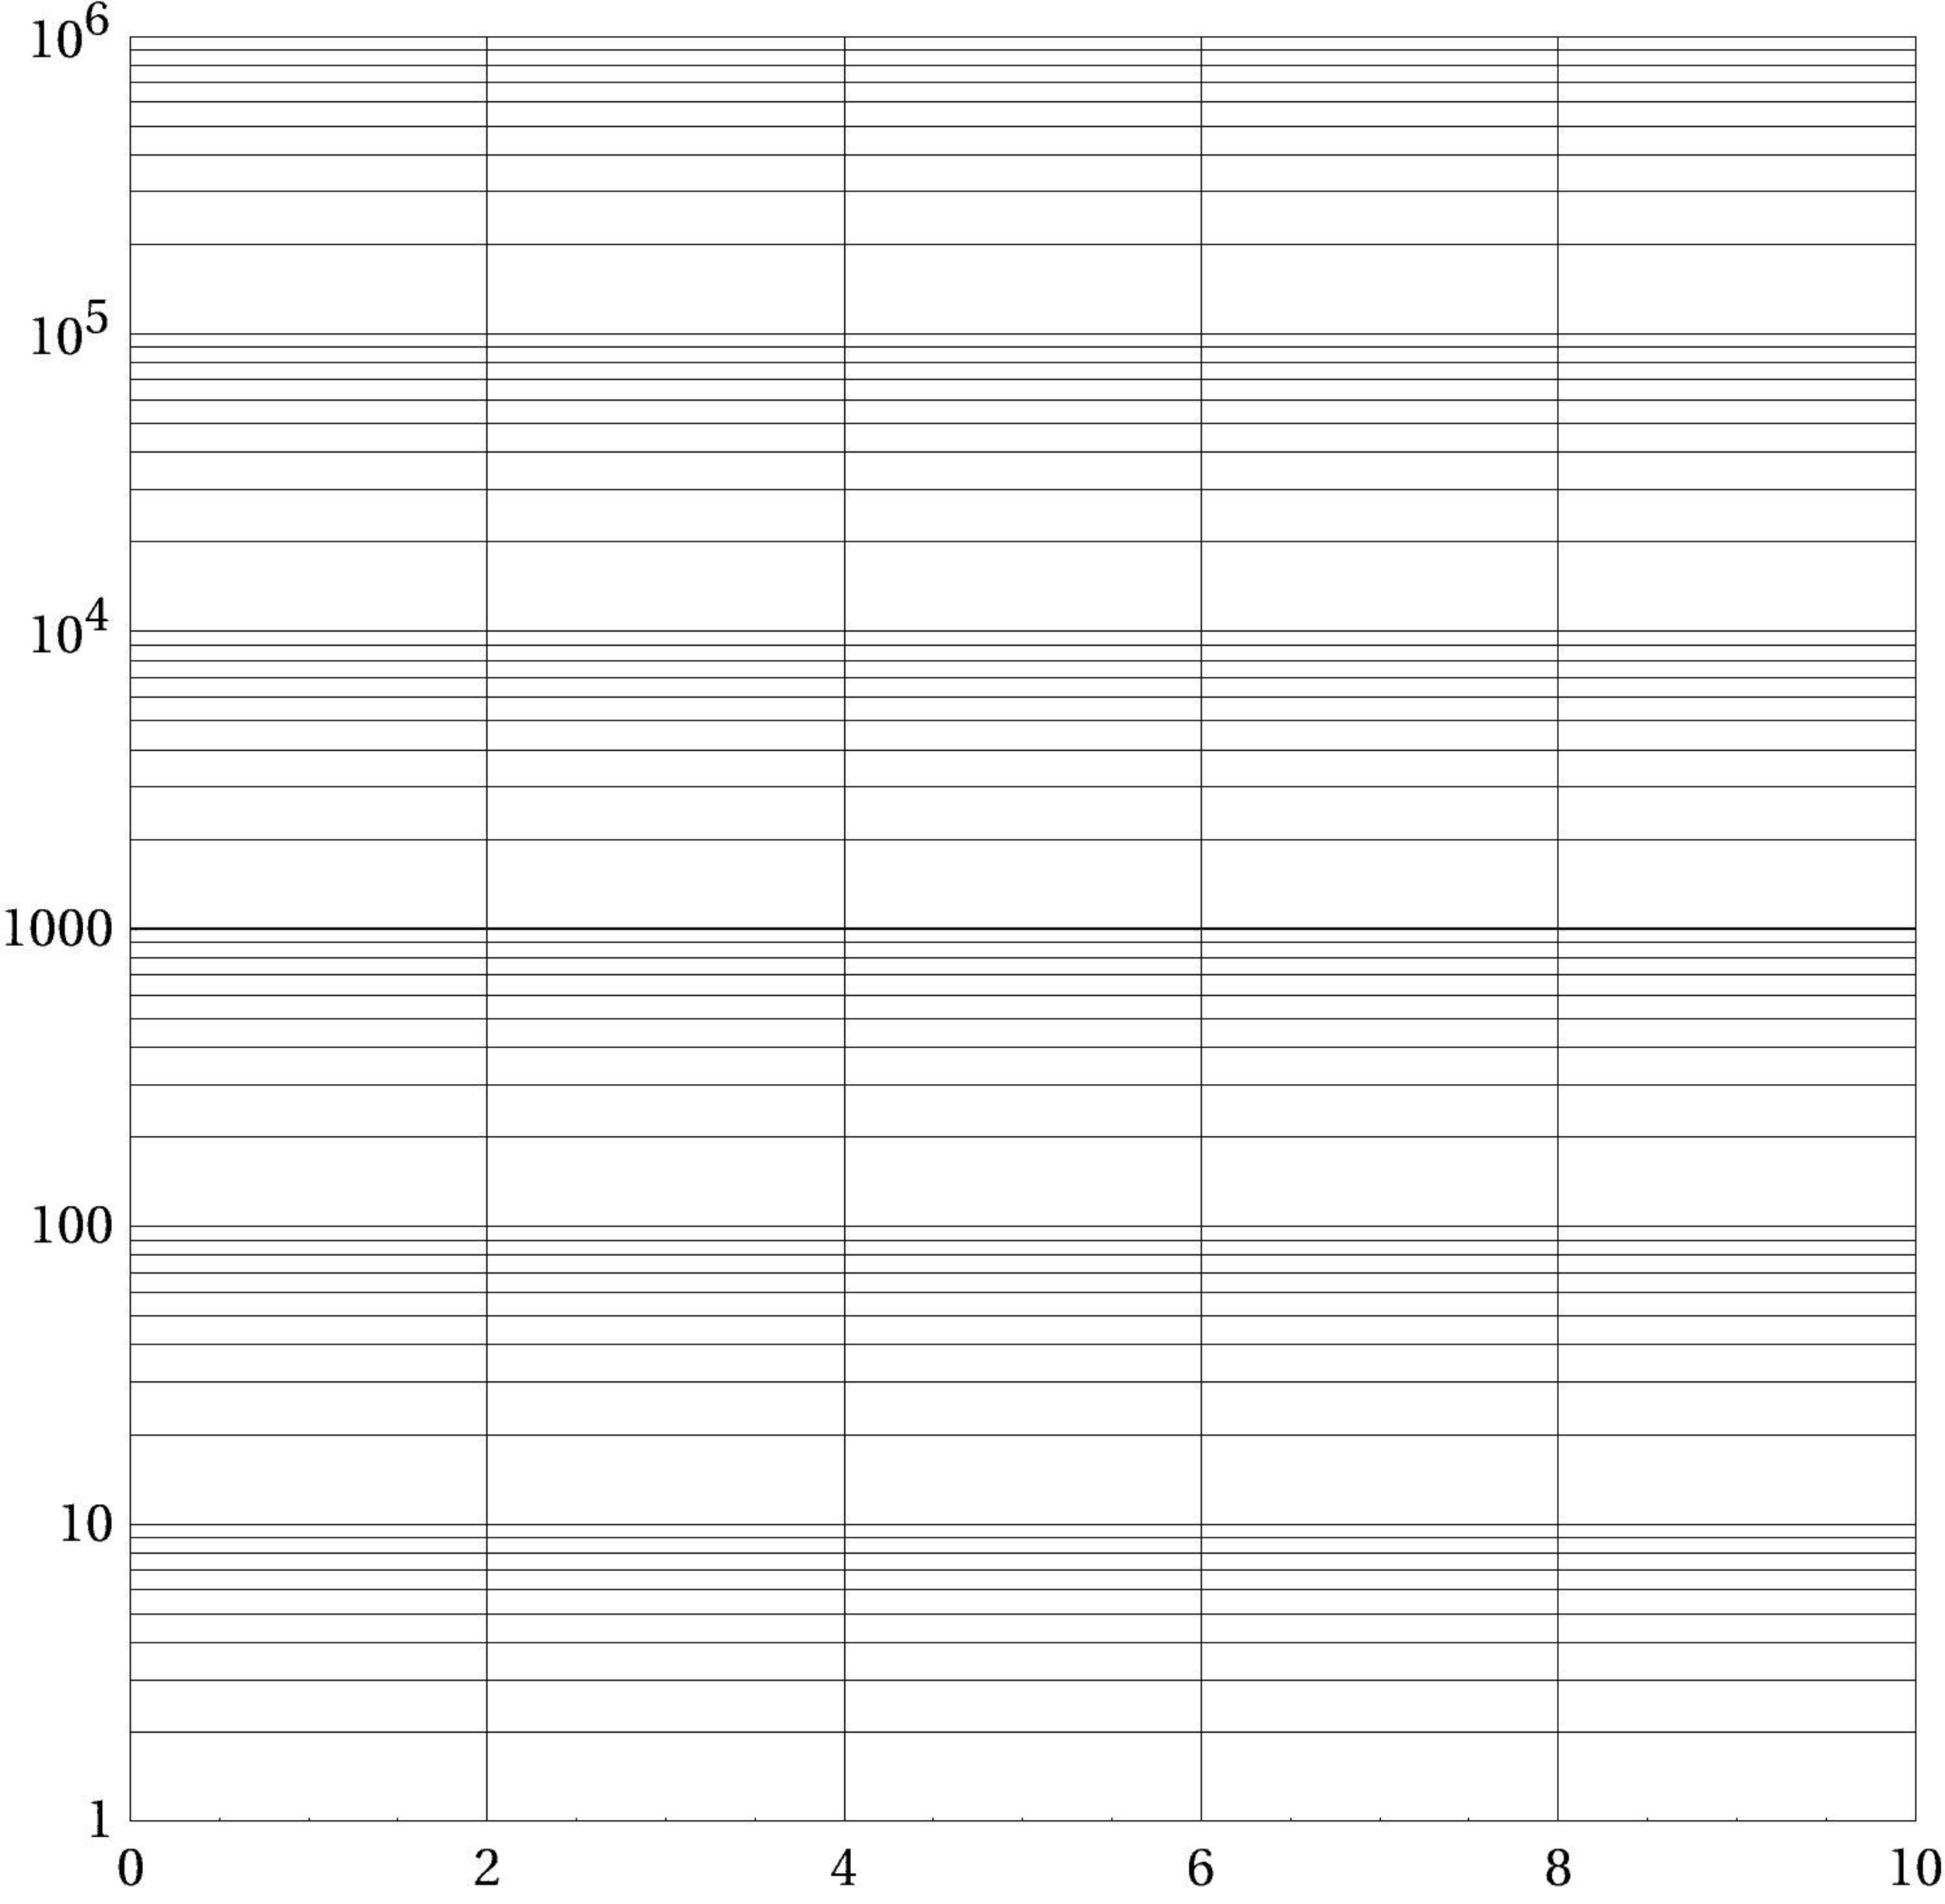
\includegraphics[width=4in]{../graphics/semiLog.pdf}
\]
\end{prob}

%\documentclass[handout]{ximera}
\documentclass[nooutcomes]{ximera}

\usepackage{gensymb}
\usepackage{tabularx}
\usepackage{mdframed}
\usepackage{pdfpages}
%\usepackage{chngcntr}

\let\problem\relax
\let\endproblem\relax

\newcommand{\property}[2]{#1#2}




\newtheoremstyle{SlantTheorem}{\topsep}{\fill}%%% space between body and thm
 {\slshape}                      %%% Thm body font
 {}                              %%% Indent amount (empty = no indent)
 {\bfseries\sffamily}            %%% Thm head font
 {}                              %%% Punctuation after thm head
 {3ex}                           %%% Space after thm head
 {\thmname{#1}\thmnumber{ #2}\thmnote{ \bfseries(#3)}} %%% Thm head spec
\theoremstyle{SlantTheorem}
\newtheorem{problem}{Problem}[]

%\counterwithin*{problem}{section}



%%%%%%%%%%%%%%%%%%%%%%%%%%%%Jenny's code%%%%%%%%%%%%%%%%%%%%

%%% Solution environment
%\newenvironment{solution}{
%\ifhandout\setbox0\vbox\bgroup\else
%\begin{trivlist}\item[\hskip \labelsep\small\itshape\bfseries Solution\hspace{2ex}]
%\par\noindent\upshape\small
%\fi}
%{\ifhandout\egroup\else
%\end{trivlist}
%\fi}
%
%
%%% instructorIntro environment
%\ifhandout
%\newenvironment{instructorIntro}[1][false]%
%{%
%\def\givenatend{\boolean{#1}}\ifthenelse{\boolean{#1}}{\begin{trivlist}\item}{\setbox0\vbox\bgroup}{}
%}
%{%
%\ifthenelse{\givenatend}{\end{trivlist}}{\egroup}{}
%}
%\else
%\newenvironment{instructorIntro}[1][false]%
%{%
%  \ifthenelse{\boolean{#1}}{\begin{trivlist}\item[\hskip \labelsep\bfseries Instructor Notes:\hspace{2ex}]}
%{\begin{trivlist}\item[\hskip \labelsep\bfseries Instructor Notes:\hspace{2ex}]}
%{}
%}
%% %% line at the bottom} 
%{\end{trivlist}\par\addvspace{.5ex}\nobreak\noindent\hung} 
%\fi
%
%


\let\instructorNotes\relax
\let\endinstructorNotes\relax
%%% instructorNotes environment
\ifhandout
\newenvironment{instructorNotes}[1][false]%
{%
\def\givenatend{\boolean{#1}}\ifthenelse{\boolean{#1}}{\begin{trivlist}\item}{\setbox0\vbox\bgroup}{}
}
{%
\ifthenelse{\givenatend}{\end{trivlist}}{\egroup}{}
}
\else
\newenvironment{instructorNotes}[1][false]%
{%
  \ifthenelse{\boolean{#1}}{\begin{trivlist}\item[\hskip \labelsep\bfseries {\Large Instructor Notes: \\} \hspace{\textwidth} ]}
{\begin{trivlist}\item[\hskip \labelsep\bfseries {\Large Instructor Notes: \\} \hspace{\textwidth} ]}
{}
}
{\end{trivlist}}
\fi


%% Suggested Timing
\newcommand{\timing}[1]{{\bf Suggested Timing: \hspace{2ex}} #1}




\hypersetup{
    colorlinks=true,       % false: boxed links; true: colored links
    linkcolor=blue,          % color of internal links (change box color with linkbordercolor)
    citecolor=green,        % color of links to bibliography
    filecolor=magenta,      % color of file links
    urlcolor=cyan           % color of external links
}

\title{Sketching Roots}
\author{Bart Snapp and Brad Findell}

\outcome{Learning outcome goes here.}

\begin{document}
\begin{abstract}
We seek to understand the connection between roots and the plots of
polynomials.
\end{abstract}
\maketitle

\label{A:sketchRoots}

In this activity we seek to better understand the connection between
roots and the plots of polynomials.  We will restrict our attention to polynomials with real coefficients.  

First, we need to be precise about the correct usage of some important language:  

\begin{itemize}
\item Expressions have \emph{values}.  
\item Equations have \emph{solutions}:  values of the variables that make the equation true. 
\item Functions have \emph{zeros}: input values that give output values of 0.
\item Polynomials (i.e., polynomial expressions) have \emph{roots}.  
\end{itemize}
These ideas are related, of course, as follows:  A zero of a polynomial function, $p(x)$, is a root of the polynomial $p(x)$ and a solution to the equation $p(x) = 0$.  

Please try to use this language correctly:  Equations do not have zeros, and functions do not have solutions.  

\begin{problem}
Give an example of a polynomial, and write a true sentence about related equations, functions, zeros, equations, and roots.  
\end{problem}

\begin{problem}
Sketch the plot of a quadratic polynomial with real coefficients that has:
\begin{enumerate}
\item Two real roots.
\item One repeated real root.
\item No real roots.
\end{enumerate}
In each case, give an example of such a polynomial.
\end{problem}

\begin{problem}
Can you have a quadratic polynomial with exactly one real root and
$1$ complex root?  Explain why or why not.
\end{problem}


\begin{problem}
Sketch the plot of a cubic polynomial with real coefficients that has:
\begin{enumerate}
\item Three distinct real roots.
\item One real root and two complex roots.
\end{enumerate}
In each case, give an example of such a polynomial.
\end{problem}

\begin{problem}
Can you have a cubic polynomial with no real roots?  Explain why or
why not. What about two distinct real roots and one complex root?
\end{problem}


\begin{problem}
For polynomials with real coefficients of degree $1$ to $5$, classify
exactly which types of roots can be found. For example, in our work
above, we classified polynomials of degree $2$ and $3$.
\end{problem}

\end{document}

%\documentclass[handout]{ximera}
\documentclass{ximera}

\usepackage{gensymb}
\usepackage{tabularx}
\usepackage{mdframed}
\usepackage{pdfpages}
%\usepackage{chngcntr}

\let\problem\relax
\let\endproblem\relax

\newcommand{\property}[2]{#1#2}




\newtheoremstyle{SlantTheorem}{\topsep}{\fill}%%% space between body and thm
 {\slshape}                      %%% Thm body font
 {}                              %%% Indent amount (empty = no indent)
 {\bfseries\sffamily}            %%% Thm head font
 {}                              %%% Punctuation after thm head
 {3ex}                           %%% Space after thm head
 {\thmname{#1}\thmnumber{ #2}\thmnote{ \bfseries(#3)}} %%% Thm head spec
\theoremstyle{SlantTheorem}
\newtheorem{problem}{Problem}[]

%\counterwithin*{problem}{section}



%%%%%%%%%%%%%%%%%%%%%%%%%%%%Jenny's code%%%%%%%%%%%%%%%%%%%%

%%% Solution environment
%\newenvironment{solution}{
%\ifhandout\setbox0\vbox\bgroup\else
%\begin{trivlist}\item[\hskip \labelsep\small\itshape\bfseries Solution\hspace{2ex}]
%\par\noindent\upshape\small
%\fi}
%{\ifhandout\egroup\else
%\end{trivlist}
%\fi}
%
%
%%% instructorIntro environment
%\ifhandout
%\newenvironment{instructorIntro}[1][false]%
%{%
%\def\givenatend{\boolean{#1}}\ifthenelse{\boolean{#1}}{\begin{trivlist}\item}{\setbox0\vbox\bgroup}{}
%}
%{%
%\ifthenelse{\givenatend}{\end{trivlist}}{\egroup}{}
%}
%\else
%\newenvironment{instructorIntro}[1][false]%
%{%
%  \ifthenelse{\boolean{#1}}{\begin{trivlist}\item[\hskip \labelsep\bfseries Instructor Notes:\hspace{2ex}]}
%{\begin{trivlist}\item[\hskip \labelsep\bfseries Instructor Notes:\hspace{2ex}]}
%{}
%}
%% %% line at the bottom} 
%{\end{trivlist}\par\addvspace{.5ex}\nobreak\noindent\hung} 
%\fi
%
%


\let\instructorNotes\relax
\let\endinstructorNotes\relax
%%% instructorNotes environment
\ifhandout
\newenvironment{instructorNotes}[1][false]%
{%
\def\givenatend{\boolean{#1}}\ifthenelse{\boolean{#1}}{\begin{trivlist}\item}{\setbox0\vbox\bgroup}{}
}
{%
\ifthenelse{\givenatend}{\end{trivlist}}{\egroup}{}
}
\else
\newenvironment{instructorNotes}[1][false]%
{%
  \ifthenelse{\boolean{#1}}{\begin{trivlist}\item[\hskip \labelsep\bfseries {\Large Instructor Notes: \\} \hspace{\textwidth} ]}
{\begin{trivlist}\item[\hskip \labelsep\bfseries {\Large Instructor Notes: \\} \hspace{\textwidth} ]}
{}
}
{\end{trivlist}}
\fi


%% Suggested Timing
\newcommand{\timing}[1]{{\bf Suggested Timing: \hspace{2ex}} #1}




\hypersetup{
    colorlinks=true,       % false: boxed links; true: colored links
    linkcolor=blue,          % color of internal links (change box color with linkbordercolor)
    citecolor=green,        % color of links to bibliography
    filecolor=magenta,      % color of file links
    urlcolor=cyan           % color of external links
}

\title{Geometry and Adding Complex Numbers}
\author{Bart Snapp and Brad Findell}

\outcome{Learning outcome goes here.}

\begin{document}
\begin{abstract}
Abstract goes here.  
\end{abstract}
\maketitle

\label{A:complexAddition}


Let's think about the geometry of adding complex numbers. We won't be
alone on our journey---Louie Llama\index{Louie Llama} is here to help
us out:
\begin{image}
\begin{tabular}{ccc}

\includegraphics[scale=.5]{llama.pdf} & 
\qquad $\leftrightsquigarrow$\qquad & 
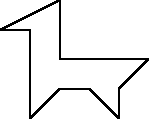
\includegraphics{llamaPlot.pdf}\\
Louie Llama & & how we'll draw him
\end{tabular}
\end{image}

\begin{problem} 
Here's Louie Llama hanging out near the point $0$ in the complex
plane. Add $4+4i$ to him. Make a table and show in the plane below what happens.
\begin{image}
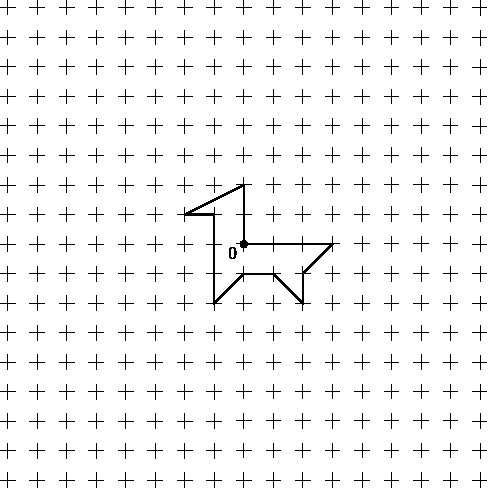
\includegraphics{complexAdd.pdf}
\end{image}
\end{problem}

\begin{problem}
Explain what it means to ``add'' a complex number to Louie
Llama. Describe the process(es) used when doing this.
\end{problem}


\begin{problem} 
Put Louie Llama back where he started, now add $1-5i$ to him.  Make a
table and show what happens in the plane.
\end{problem}


\begin{problem} 
Geometrically speaking, what does it mean to ``add'' complex numbers?
\end{problem}

\end{document}

%\documentclass[handout]{ximera}
\documentclass{ximera}

\usepackage{gensymb}
\usepackage{tabularx}
\usepackage{mdframed}
\usepackage{pdfpages}
%\usepackage{chngcntr}

\let\problem\relax
\let\endproblem\relax

\newcommand{\property}[2]{#1#2}




\newtheoremstyle{SlantTheorem}{\topsep}{\fill}%%% space between body and thm
 {\slshape}                      %%% Thm body font
 {}                              %%% Indent amount (empty = no indent)
 {\bfseries\sffamily}            %%% Thm head font
 {}                              %%% Punctuation after thm head
 {3ex}                           %%% Space after thm head
 {\thmname{#1}\thmnumber{ #2}\thmnote{ \bfseries(#3)}} %%% Thm head spec
\theoremstyle{SlantTheorem}
\newtheorem{problem}{Problem}[]

%\counterwithin*{problem}{section}



%%%%%%%%%%%%%%%%%%%%%%%%%%%%Jenny's code%%%%%%%%%%%%%%%%%%%%

%%% Solution environment
%\newenvironment{solution}{
%\ifhandout\setbox0\vbox\bgroup\else
%\begin{trivlist}\item[\hskip \labelsep\small\itshape\bfseries Solution\hspace{2ex}]
%\par\noindent\upshape\small
%\fi}
%{\ifhandout\egroup\else
%\end{trivlist}
%\fi}
%
%
%%% instructorIntro environment
%\ifhandout
%\newenvironment{instructorIntro}[1][false]%
%{%
%\def\givenatend{\boolean{#1}}\ifthenelse{\boolean{#1}}{\begin{trivlist}\item}{\setbox0\vbox\bgroup}{}
%}
%{%
%\ifthenelse{\givenatend}{\end{trivlist}}{\egroup}{}
%}
%\else
%\newenvironment{instructorIntro}[1][false]%
%{%
%  \ifthenelse{\boolean{#1}}{\begin{trivlist}\item[\hskip \labelsep\bfseries Instructor Notes:\hspace{2ex}]}
%{\begin{trivlist}\item[\hskip \labelsep\bfseries Instructor Notes:\hspace{2ex}]}
%{}
%}
%% %% line at the bottom} 
%{\end{trivlist}\par\addvspace{.5ex}\nobreak\noindent\hung} 
%\fi
%
%


\let\instructorNotes\relax
\let\endinstructorNotes\relax
%%% instructorNotes environment
\ifhandout
\newenvironment{instructorNotes}[1][false]%
{%
\def\givenatend{\boolean{#1}}\ifthenelse{\boolean{#1}}{\begin{trivlist}\item}{\setbox0\vbox\bgroup}{}
}
{%
\ifthenelse{\givenatend}{\end{trivlist}}{\egroup}{}
}
\else
\newenvironment{instructorNotes}[1][false]%
{%
  \ifthenelse{\boolean{#1}}{\begin{trivlist}\item[\hskip \labelsep\bfseries {\Large Instructor Notes: \\} \hspace{\textwidth} ]}
{\begin{trivlist}\item[\hskip \labelsep\bfseries {\Large Instructor Notes: \\} \hspace{\textwidth} ]}
{}
}
{\end{trivlist}}
\fi


%% Suggested Timing
\newcommand{\timing}[1]{{\bf Suggested Timing: \hspace{2ex}} #1}




\hypersetup{
    colorlinks=true,       % false: boxed links; true: colored links
    linkcolor=blue,          % color of internal links (change box color with linkbordercolor)
    citecolor=green,        % color of links to bibliography
    filecolor=magenta,      % color of file links
    urlcolor=cyan           % color of external links
}

\title{Geometry and Multiplying Complex Numbers}
\author{Bart Snapp and Brad Findell}

\outcome{Learning outcome goes here.}

\begin{document}
\begin{abstract}
Abstract goes here.  
\end{abstract}
\maketitle

\label{A:complexMultiplication}

Now we'll investigate the geometry of multiplying complex
numbers. In each case, specify the transformation.  For example, if you see a rotation, specify the angle and the center of rotation.  

Louie Llama\index{Louie Llama} is here to help us out:
\begin{image}
\begin{tabular}{ccc}

\includegraphics[scale=.5]{llama.pdf} & 
\qquad $\leftrightsquigarrow$\qquad & 
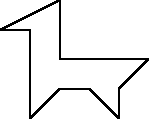
\includegraphics{llamaPlot.pdf}\\
Louie Llama & & how we'll draw him
\end{tabular}
\end{image}

\begin{problem} 
Here's Louie Llama hanging out near the point $0$ in the complex
plane. Multiply him by $2$. Make a table and show in the plane below what happens.  What transformation do you see?  
\begin{image}
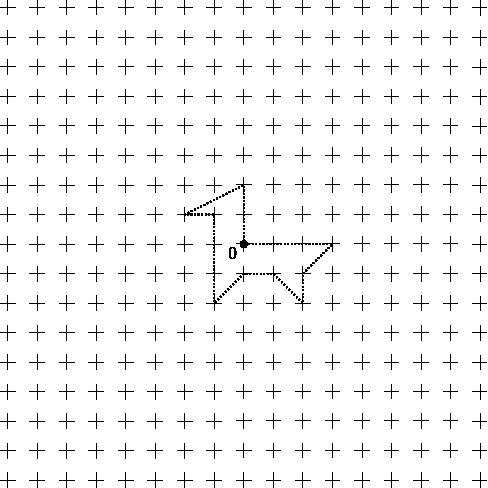
\includegraphics{complexMult.pdf}
\end{image}
\end{problem}

\begin{problem} 
Now multiply him by $i$. Make a table and show in the plane below what happens.  What transformation do you see?  
\begin{image}

\includegraphics{complexPlane.pdf}
\end{image}
\end{problem}

\vfill

\begin{problem} 
Now multiply Louie Llama by $1+i$. Make a table and show in the plane
below what happens.  What transformation do you see?  
\begin{image}

\includegraphics{complexPlane.pdf}
\end{image}
\end{problem}

\vfill


\begin{problem} 
%  Used to mutliply by $\frac{1}{2}+\frac{\sqrt{3}}{2}i$.
Now multiply Louie Llama by $1 - 2i$. Make a
table and show in the plane below what happens.  What transformation do you see?  
\begin{image}

\includegraphics{complexPlane.pdf}
\end{image}
\end{problem}


\begin{problem}
Make a table to summarize your results from the previous problems.  
Then describe what happens geometrically when we ``multiply''  by a complex
number. 
\end{problem}

\end{document}

%\newpage
\section{To the Second Degree}\label{A:deg2Ext}

In this activity, we seek to understand why roots of polynomials with
real coefficients must always come in conjugate pairs.

\begin{prob}
Consider your favorite (non-real) complex number, I'll call it
$\xi$. Find a polynomial with real coefficients whose degree is as
small as possible having your number as a root. What is the degree
of your polynomial?
\end{prob}


\begin{prob}
I'll call the polynomial found in the first problem $s(x)$. Let $f(x)$
be some other polynomial with
\[
f(\xi) = 0.
\]
I claim $s(x) | f(x)$. Explain why if $s(x)\nmid f(x)$ then there exist $q(x)$ and $r(x)$ with
\[
f(x) = s(x) \cdot q(x) + r(x)\qquad\text{with }\deg(r) <\deg(s).
\]
\end{prob}

\begin{prob}
Plug in $\xi$ for $x$ in the equation above. What does this tell you
about $r(\xi)$? Is this possible?
\end{prob}

\begin{prob}
Explain why complex roots must always come in conjugate pairs. Also
plot some conjugate pairs in the complex plane and explain what
``conjugation'' means geometrically.
\end{prob}

%\newpage
\section{Undoing---Using Inverse Functions}



\begin{prob}
Formulas are fine, but what do you do to solve something like this:
\[
5 = e^x \qquad \text{}
\]
\end{prob}





and To Infinity and Beyond!)

What about equations that can't be put (or easily) put into a nice
form?  They might have solutions too, but if we only rely on the
``undoing'' means, we may never find them (and thus, all most students
are given in school are those ``rigged up'' equations- yes- important
to know how to solve, but they're not the only ones around)!  For
example, if you involve two or more types of functions in the same
equation (say exponential, log, and polynomial- e.g., $5\cdot
2^{x-4}-x^13 + \ln(x) + 102.8=0$), you now have several different
kinds of ``undoings'' to contend with.

Over the centuries, methods have been developed to deal with the
``ugly'' cases mentioned in the paragraph above.  Usually, we only end
up with an approximate answer, but we can often dictate how close the
answer can be to the actual (by analyzing the algorithms and figuring
out how many steps would be necessary to get as close as we need to
be).

\paragraph{Graphing Calculator} 
With the advent of powerful technology, we can often sidestep many of
these mathematical issues with even a simple hand-held graphing
calculator (which probably has a ``solve'' feature that will (usually)
give you a solution closest to a value you give it (if a solution
exists)).  You can also do a little more yourself by using the
graphing feature and (best done by bringing everything over = 0 and
enter the function on the other side and find its x-intercepts by
using the ``zoom'' feature).  Side question, though: How is the
calculator doing these things?  How was it programmed?  What
mathematical methods is it using?

However, you can also do a few other techniques that require a bit
more work.  For example:

\paragraph{Judicious Guess and Check}  
Don't underestimate this technique, which is the first technique that
we really should start with in early childhood (e.g., ``Fill in the
brackets: $15-\langle\, \rangle=6$''.  Before knowing any ``undoing''
techniques, we guess and check judiciously until we see that $9$ is what
makes the statement true- perhaps using objects and/or couching it in
a story problem.).  It can also lead to an expression(s) to model the
story problem if you can't already find one (perhaps it helped you in
the \textit{Dreaded Story Problem} to do just that!).  

For solving the equations that are wacky like the one above that
involved a lot of function types, we basically do the same as the
early childhood student (with a little more background) and can use
the calculator to do the grungy calculating for us.  Enter and guess
our first solution to be, say, 4 and see if that gives us zero when we
plug it in.  Unfortunately, $f(4) = -67108754.81$, which apparently is
not zero!  But we guess again and plug in, say, 1 and we get $f(1) =
102.425$.  I claim that we can guarantee that there is a solution
between $x = -1$ and $x = 4$ (why?).  Now hone in on that solution (or
maybe even find others in that interval).  We'll do the ``bisection''
technique here, which means we'll test the midpoint between $1$ and $4$
(and all midpoints of subsequent intervals): 2.5: $f(2.5) \approx -150000$. So, we have an answer between 1 and 2.5 (why?).  Try $f(1.75)=
-1339.348$.  Try 1.375 (midpoint between 1 and 1.75); $f(1.375)=41.132$,
which is greater than zero, so our answer must be between 1.375 and
1.75.  Try that midpoint: 1.5625: $f(1.5625)=-226.703<0$.  So the answer
must be between 1.375 and 1.5625: try 1.46875: $f(1.46875)=-43.9713<0$.
So we know our answer must be between 1.46875 and 1.375.  And so on
until we get the accuracy we need.  There are several variations on
this technique (in terms of how to find your next guess.  Here we
always used the midpoint).

\paragraph{Fixed Point Iteration} 
(You might look at the activity ``Spreadsheet Mania'' before embarking
on this method).  Often, when teaching algebra to students who only
know how to solve linear equations, I will find students who make an
initial stab at solving, say, a quadratic equation for $x$, in the
following manner:
\begin{align*}
x^2 + 2x -8 &= 0 & \\
2x &= 8 - x^2 & \\
x &= 4- .5 x^2 & \text{(divided by $2$)}
\end{align*}
Or, they will do something like this:
\begin{align*}
x^2 + 2x -8 &= 0 \\
x(x+2) &= 8 \\
x = \frac{8}{x+2}
\end{align*}
Of course, this seems pointless, as we don't get an equation of the
tried and true form ``x = a number''.  Instead, we get 
\[
x= \text{another expression in terms of $x$} 
\]
or ``x = g(x).'' What should we do with such students?  Suspend or
expel them???! Actually, the students are not wrong (other than not
finding a numerical answer).  These are re-writings (``interior
decorating'') of the original equation.  But what good are they?

It turns out that, under certain conditions, we can take advantage of
this form to get a solution (but not necessarily all solutions) by
using this form $g(x)=x$ and plugging in an initial value into $g(x)$
and plugging the result back into g(x), and so on.  Under certain
conditions, the values will approach a solution (i.e., we keep getting
roughly the same value over and over, meaning the $g(x)$ we're getting
is the same as the $x$ we'll plug in next, thus satisfying the
original equation).  And it's a nice method for when $x$ can be solved
for using traditional algebraic techniques (``undoing''), but just not
for a number.
      
You can use your calculator or (much quicker yet) the spreadsheet to
do this (How is this related to recursion??).
      
In our example, we already know the solutions to the equation from previous schoolwork.  That is, $x = 2$ and $x = - 4$.
\begin{enumerate}
\item Use $x=\frac{8}{x+2}$ .  Start with $x = 4$ and plug it into the right side (the initial value is often called the ``seed'').  We get $8/6= 1.\bar{3}$.  Now plug $1.\bar{3}$ into the same expression and get $2.4$.  Then plug in $2.4$ into it, etc., etc.  Keep doing this about 10 times (10 iterations) and you'll notice that the resulting values bounce before and after 2, one of our known solutions.  In fact, you'll find that no matter what your seed is (even, say, -4000), you'll relatively quickly be converging to 2.  However, no seed will get you close to the other solution (-4).  (How can this be done on a spreadsheet?: See the later activity ``Spreadsheet Mania'' for a good shortcut method to avoid the drudgery you've experienced)
\item Try the other ``solution'' we came up with in the intro:  $g(x) = 4-.5x^2$  Try it, no matter what you put in for your seed or the number of iterations, it won't get close to either solution (in fact, it sometimes will ``blow up'').  Thus, some forms are better than others for this method.
\item Say we wanted to solve $x^3 – 3x = 0$.  (We can do this
conventionally by factoring out $x$ and getting $0$, and +/- square root
of 3 (about 1.732)).  We can also ``solve for x'' and get $x = x^3 –
2x$.  Using $x^3-2x$ as our $g(x)$, use 1 as your seed and what happens?
Will any seed or \# of iterations get us reasonably close to the known
roots?  Try an alternative: $x = (1/3)x^3$. (Try seeds = 1.732, 1.735,
1.738.  What happened?  Try seed=1.7.  What happened?)  

\item Try another quadratic equation (known solutions again): $x^2+9x+19 = 0$.  Solve for $x = -19/(x+9)$ and use several seeds.  Do you get close to a solution?
Which one?  

\item Now solve an equation we have no idea about a solution
for: $x^2 – \cos(x) = 0.$  Solving for $x$ gives $x = \sqrt{\cos(x)}$.  Can you
conjecture a solution?  Check that it works in the original equation
on a calculator. 
\item When does this ``fixed point'' technique work?
Put the graphs of our $g(x)$'s with the graph $y=x$ (Why would this make
sense to do?).  Because we're not as familiar with some of the $g(x)$'s,
let's use g(x) = linear graphs first.  Use the spreadsheet as well:
Use $g(x) = 2x +3, -2x + 3, .7x + 3, 1.1x +3, .92x + 3$., etc. with
several seeds.  You'll have to fill down quite a ways (say 1000) to
see what's happening.  Sketch the graph of each with y=x and see what
happens graphically.  Make a conjecture as to when fixed point
iteration works or not.  

\item This idea of ``fixed point'' is
generalized to more powerful equation solving algorithms, including
Newton's Method.  It is generalized even more to solving other kinds
of equations, such as differential equations.
\end{enumerate}
\paragraph{Calculus-Based Techniques} For you calculus fans out there, another famous equation-solving method is ``Newton's Method''.  It's reasonably simple to understand- just need to see a picture involving tangent lines to see the reasoning. We might visit this in Math 111.

%\newpage
\section{Yet Another Division Theorem}\label{gaussianInt}


Take a minute to recall the \textit{Division Theorem}. Got it? OK we
can do something similar with complex numbers. Check this out:

\begin{definition}\index{Gaussian integers} 
A \textbf{Gaussian integer} is a number of the form
\[
a + bi
\]
where $a$ and $b$ are integers and $i$ is the square-root of negative
one.
\end{definition}

Just like with integers, we have a division theorem here too, check it
out (this time I'll play nice):

\begin{theorem}[Division Theorem]\index{Division Theorem!for Gaussian integers}
Given any Gaussian integer $\alpha$ and a nonzero Gaussian integer
$\beta$, there exist Gaussian integers $\theta$ and $\rho$ such that
\[
\alpha = \beta \cdot \theta + \rho \qquad \text{with}\qquad 
\rho\cdot\bar{\rho} <  \beta\cdot\bar{\beta}
\]
where $\bar{a + bi} = a - bi$.
\end{theorem}

Suppose you want to divide $7+7i$ by $1+2i$ and end up with quotient
and remainder that are both Gaussian integers. How do you do this?
We'll use the complex plane to help us out.
\[

\includegraphics{../graphics/complexPlane.pdf}
\]
\begin{prob} 
Mark $1+2i$ and $7 +7i$ on the complex plane. Use the grid above to
help you and be sure to label your work.
\end{prob}

\begin{prob}
Mark every Gaussian integer multiple of $1+2i$ on the plane
above. Explain what happens and explain why it happens.
\end{prob}


\begin{prob} 
Find the nearest multiple of $1+2i$ to $7+7i$.
\end{prob}

\begin{prob}
Use your work above to help find $\theta$ and $\rho$ such that
\[
7 + 7i  = (1+2i)\cdot \theta + \rho \qquad \text{with}\qquad 
\rho\cdot\bar{\rho} <  5.
\]
\end{prob}

\begin{prob}
Are the $\theta$ and $\rho$ you found above unique? Discuss.
\end{prob}

\begin{prob} 
Explain what is going on here in terms of geometry.
\end{prob}

\begin{prob}
Find $\theta$ and $\rho$ such that
\[
9 + 8i  = (5+2i)\cdot \theta + \rho \qquad \text{with}\qquad 
\rho\cdot\bar{\rho} <  29.
\]
As a gesture of friendship, I have provided a fresh grid for your
work.
\[

\includegraphics{../graphics/complexPlane.pdf}
\]
\end{prob}



\begin{prob}
Are the $\theta$ and $\rho$ you found above unique? Discuss.
\end{prob}

%\newpage
\section{Broken Records}\label{A:orderMod}

Fill in the following table:
\[
{\renewcommand{\arraystretch}{1.8}
\renewcommand{\arraycolsep}{3mm}
\begin{array}{|r||c|c|c|c|c|c|c|c|c|c|}\hline
\text{modulus:} & 2 & 3 & 4 & 5 & 6 & 7 & 8 & 9 & 10 & 11 \\ \hline\hline
2\cdot 1 \equiv & & & & & & & & & & \\ \hline
2\cdot 2 \equiv & & & & & & & & & & \\ \hline
2\cdot 3 \equiv & & & & & & & & & & \\ \hline
2\cdot 4 \equiv & & & & & & & & & & \\ \hline
2\cdot 5 \equiv & & & & & & & & & & \\ \hline
2\cdot 6 \equiv & & & & & & & & & & \\ \hline
2\cdot 7 \equiv & & & & & & & & & & \\ \hline
2\cdot 8 \equiv & & & & & & & & & & \\ \hline
2\cdot 9 \equiv & & & & & & & & & & \\ \hline
2\cdot 10\equiv & & & & & & & & & & \\ \hline
2\cdot 11\equiv & & & & & & & & & & \\ \hline
\end{array}}
\]

\begin{prob} 
Find patterns in your table above, clearly describe the patterns you find.
\end{prob}

\begin{prob} 
Consider the patterns you found. Can you explain why they happen?
\end{prob}

\begin{prob}
When does a column have a $0$? When does a column have a $1$? 
\end{prob}

\begin{prob}
Describe what would happen if you extend the table for bigger
moduli and bigger multiplicands.
\end{prob}


\vfill

\newpage


\[
{\renewcommand{\arraystretch}{1.8}
\renewcommand{\arraycolsep}{3mm}
\begin{array}{|r||c|c|c|c|c|c|c|c|c|c|}\hline
\text{modulus:} & 2 & 3 & 4 & 5 & 6 & 7 & 8 & 9 & 10 & 11 \\ \hline\hline
3\cdot 1 \equiv & & & & & & & & & & \\ \hline
3\cdot 2 \equiv & & & & & & & & & & \\ \hline
3\cdot 3 \equiv & & & & & & & & & & \\ \hline
3\cdot 4 \equiv & & & & & & & & & & \\ \hline
3\cdot 5 \equiv & & & & & & & & & & \\ \hline
3\cdot 6 \equiv & & & & & & & & & & \\ \hline
3\cdot 7 \equiv & & & & & & & & & & \\ \hline
3\cdot 8 \equiv & & & & & & & & & & \\ \hline
3\cdot 9 \equiv & & & & & & & & & & \\ \hline
3\cdot 10\equiv & & & & & & & & & & \\ \hline
3\cdot 11\equiv & & & & & & & & & & \\ \hline
\end{array}}
\]

\begin{prob} 
Find patterns in your table above, clearly describe the patterns you find.
\end{prob}

\begin{prob} 
Consider the patterns you found. Can you explain why they happen?
\end{prob}


\begin{prob}
When does a column have a $0$? When does a column have a $1$? 
\end{prob}


\begin{prob}
Can you describe what would happen if you extend the table for bigger
moduli and bigger multiplicands?
\end{prob}

\begin{prob}
Describe precisely when a column of the table will contain
representatives for each integer modulo $n$. Explain why your
description is true.
\end{prob}


%\newpage
\section{Close, but No Cigar}

Sometimes, we are not able to come up with formulas for our function
models.  In fact, sometimes all that we have are a few data points $(x,
y)$.  Obviously, we'd like to know more exact values of our function,
but the cupboard is often bare---we have to make lemonade out of
lemons.  Thus, we try to ``fill in'' points in between the given points
in order for our model to have some predictive quality to it.

You already saw this in Statistics 145 when you talked about the
``best-fit'' line.  There actually could be several definitions of what
is meant by this, but typically we use the ``least-squares'' line.
Although we usually see the formula for the slope and intercept of
this line either just quoted or derived with multi-variable calculus
in textbooks (something probably not done with the limited time
allotted for Math 111), you can actually find it for yourself using
algebraic ideas from school (although it also would be nice to know
why those algebraic ideas work!):

\begin{prob}
Find the ``least-squares'' line for the data points $(2, 3)$, $(4,
5)$, and $(6, 11)$ (note that these don't already form a line- graph
or algebraically see or just use common sense): That is, find $a$ and
$b$ so that the sum of the squares of the vertical distances of the
above data points from the line $y=ax+b$ is as small as possible
(Unpack what these words really say---a graph is probably best!  Then
solve algebraically using what you know from Algebra II or so).
\end{prob}

\begin{prob}
Of course, contrary to the ``linear disease'' that engulfs our
country, not every variable grows at the same rate all the time (i.e.,
we're not always on cruise control or, mathematically, not every
relationship is linear!)!  If the data you're given appear to be
non-linear, we try to fit a predictive non-linear curve to such a
graph (e.g., if the graph appears to be exponential in nature, we try
to fit a ``best-fit exponential function'' $y=ke^{ax}$ instead of a
``best-fit'' line $y=ax+b$).  Now how can you tell if a graph appears
to be exponential or more like a polynomial?  For example, look at the
data below:
\[
\begin{array}{|c|c|c|c|c|}\hline
x & 0 & 1 & 2 & 3 \\ \hline
y & 8.1 & 22.1 & 60.1 & 165 \\ \hline
\end{array}
\]

A group of students graph the data.  Susie says, ``This sure looks
like a parabola!''  But Fred says, ``No it doesn't, I just got done
studying exponentials and it looks like an exponential!''  Susie says
in reply, ``What?! I sat in those boring classes with you---I know
about exponentials, but I also know my parabolas---and this is a
parabola.''  Then Julie chimes in, ``Both of you dummies are wrong,
it's a quartic ($x^4$)''.  Then a whole slew of ``Says who? Says me!''
ensues.  Before this turns into a brawl and people get hurt, how can
we sanely tell who is right, if any of them? They can't all be right!


Hint: Think about the most famous graph of all, the one you know most
about.  And see if you can somehow convert the above data to get that
type of graph by graphing the relationship between variables related
to $x$ and $y$ That is, if it was truly best modeled by $y=ke^{ax}$,
then we'd know (why?) $\ln(y) = ax \ln(k)$ (try graphing the
$x$-coordinates on the horizontal axis and the natural log of the $y$
coordinates on the vertical axis. What should that graph look like if
it is best modeled by an exponential?).  If it were best modeled by $y
= kx^a$ (i.e., like a polynomial), then we'd know (why?) $\ln(y) =
a\ln(x) + \ln(k)$ (what would you graph on each axis here?).  Graph
each of these with the given data and see what happens (and find best
values for either $k$ or $a$ for the model you conjecture is best.  Note:
We could ask you to find the ``best-fit'' line for the ``linearized'' data
like in \#1, but we'll give you a break and just ask for a good eyeball
estimate here!)).

Now do the same with this data:
\[
\begin{array}{|c|c|c|c|c|}\hline
x & 1 & 2 & 3 & 4 \\ \hline
y & 8.3 & 443.6 & 24420.8 & 1364278.6 \\ \hline
\end{array}
\]

Now do the same with this data:
\[
\begin{array}{|c|c|c|c|c|c|}\hline
x & 1 & 2 & 3 & 4 & 5 \\ \hline
y & 7 & 62 & 220 & 506 & 1012 \\ \hline 
\end{array}
\]
\end{prob}

\begin{prob}
Although not all data are modeled by polynomials, because of their
easy function evaluations (place value, all K-8 arithmetic!) and
smoothness of graphs, polynomials are often a universal go-to model
for data (we try to fit a polynomial that contains all the data
points).  As was noted in Polly Nomial \#3, there are a couple of ways
to do this, at least one of which you'll do in a future activity.

Note: sometimes, finding ``best-fit'' curves can be done by a graphing
calculator (On the TI-83 and its kin, go to STATS, enter your
(2-variable) data into EDIT, and go to CALC (where you'll find LinReg,
CubicReg (cubic polynomial), ExpReg , etc.)  Of course, the
graphing calculator will blindly give you the ``best-fit'' curve of
all ilk's.  It still takes, as illustrated above, a human mind to
figure out which, if any, best fit the given data.for purposes of
prediction.
\end{prob}

%\documentclass[handout]{ximera}
\documentclass[nooutcomes]{ximera}

\usepackage{gensymb}
\usepackage{tabularx}
\usepackage{mdframed}
\usepackage{pdfpages}
%\usepackage{chngcntr}

\let\problem\relax
\let\endproblem\relax

\newcommand{\property}[2]{#1#2}




\newtheoremstyle{SlantTheorem}{\topsep}{\fill}%%% space between body and thm
 {\slshape}                      %%% Thm body font
 {}                              %%% Indent amount (empty = no indent)
 {\bfseries\sffamily}            %%% Thm head font
 {}                              %%% Punctuation after thm head
 {3ex}                           %%% Space after thm head
 {\thmname{#1}\thmnumber{ #2}\thmnote{ \bfseries(#3)}} %%% Thm head spec
\theoremstyle{SlantTheorem}
\newtheorem{problem}{Problem}[]

%\counterwithin*{problem}{section}



%%%%%%%%%%%%%%%%%%%%%%%%%%%%Jenny's code%%%%%%%%%%%%%%%%%%%%

%%% Solution environment
%\newenvironment{solution}{
%\ifhandout\setbox0\vbox\bgroup\else
%\begin{trivlist}\item[\hskip \labelsep\small\itshape\bfseries Solution\hspace{2ex}]
%\par\noindent\upshape\small
%\fi}
%{\ifhandout\egroup\else
%\end{trivlist}
%\fi}
%
%
%%% instructorIntro environment
%\ifhandout
%\newenvironment{instructorIntro}[1][false]%
%{%
%\def\givenatend{\boolean{#1}}\ifthenelse{\boolean{#1}}{\begin{trivlist}\item}{\setbox0\vbox\bgroup}{}
%}
%{%
%\ifthenelse{\givenatend}{\end{trivlist}}{\egroup}{}
%}
%\else
%\newenvironment{instructorIntro}[1][false]%
%{%
%  \ifthenelse{\boolean{#1}}{\begin{trivlist}\item[\hskip \labelsep\bfseries Instructor Notes:\hspace{2ex}]}
%{\begin{trivlist}\item[\hskip \labelsep\bfseries Instructor Notes:\hspace{2ex}]}
%{}
%}
%% %% line at the bottom} 
%{\end{trivlist}\par\addvspace{.5ex}\nobreak\noindent\hung} 
%\fi
%
%


\let\instructorNotes\relax
\let\endinstructorNotes\relax
%%% instructorNotes environment
\ifhandout
\newenvironment{instructorNotes}[1][false]%
{%
\def\givenatend{\boolean{#1}}\ifthenelse{\boolean{#1}}{\begin{trivlist}\item}{\setbox0\vbox\bgroup}{}
}
{%
\ifthenelse{\givenatend}{\end{trivlist}}{\egroup}{}
}
\else
\newenvironment{instructorNotes}[1][false]%
{%
  \ifthenelse{\boolean{#1}}{\begin{trivlist}\item[\hskip \labelsep\bfseries {\Large Instructor Notes: \\} \hspace{\textwidth} ]}
{\begin{trivlist}\item[\hskip \labelsep\bfseries {\Large Instructor Notes: \\} \hspace{\textwidth} ]}
{}
}
{\end{trivlist}}
\fi


%% Suggested Timing
\newcommand{\timing}[1]{{\bf Suggested Timing: \hspace{2ex}} #1}




\hypersetup{
    colorlinks=true,       % false: boxed links; true: colored links
    linkcolor=blue,          % color of internal links (change box color with linkbordercolor)
    citecolor=green,        % color of links to bibliography
    filecolor=magenta,      % color of file links
    urlcolor=cyan           % color of external links
}

\title{On the Road}
\author{Bart Snapp and Brad Findell}

\outcome{Learning outcome goes here.}

\begin{document}
\begin{abstract}
  We find binomial coefficients in unexpected places.
\end{abstract}
\maketitle

\label{A:traffic}

\begin{problem} 
Steve likes to drive the city roads. Suppose he is driving down a road
with three traffic lights. For this activity, we will ignore yellow
lights, and pretend that lights are either red or green.
\begin{enumerate}
\item How many ways could he see one red light and two green lights?
\item How many ways could he see one green light and two red lights?
\item How many ways could he see all red lights?
\end{enumerate}
\end{problem}

\begin{problem} 
Now suppose Steve is driving down a road with four traffic lights.
\begin{enumerate}
\item How many ways could he see two red light and two green lights?
\item How many ways could he see one green light and three red lights?
\item How many ways could he see all green lights?
\end{enumerate}
\end{problem}

\begin{problem} 
In the following chart let $n$ be the number of traffic
lights and $k$ be  the number of green lights seen. In each square, write the number of ways this number of green lights could be seen while Steve drives down the street.
\newpage

\begin{teachingnote}
It is hard for students to see the patterns.  But sheering the table might make it easy to recognize as Pascal's triangle, and then some students will fill it in rotely rather than spending their intellectual energy on careful, organized counting of the possibilities.  

Don't worry about $n = k = 0$ at this point.  But when $k > n$ the entry clearly should be $0$. 
\end{teachingnote}
\[
\begin{array}{|c|c|c|c|c|c|c|c|}
    \hline
          & k=0 & k=1 & k=2 & k=3 & k=4 & k=5 & k = 6\\
    \hline
    n=0 &\rule[0mm]{0mm}{7mm}&       &       &       &       &   &   \\
    \hline
    n=1 &\rule[0mm]{0mm}{7mm}  &       &       &       &       &   &   \\
    \hline
    n=2 & \rule[0mm]{0mm}{7mm} &     &     &       &       &    &  \\
    \hline
    n=3 &\rule[0mm]{0mm}{7mm}       &       &       &       &       &   &   \\
    \hline
    n=4 & \rule[0mm]{0mm}{7mm}      &       &       &       &       &   &   \\
    \hline
    n=5 &\rule[0mm]{0mm}{7mm}       &       &       &       &       &   &   \\
    \hline
    n=6 &\rule[0mm]{0mm}{7mm}       &       &       &       &       &   &   \\
    \hline
\end{array}
\]
Describe any patterns you see in your table and try to explain them in
terms of traffic lights.
\begin{teachingnote}
Let $\binom{n}{k}$ denote the entry in the $n^{th}$ row and $k^{th}$ column.  Then we hope that students will notice patterns such as the following: 
\begin{itemize}
\item $\binom{n}{0} = \binom{n}{n} = 1$
\item $\binom{n}{1} = n$
\item $\binom{n}{k} = \binom{n}{n-k}$
\end{itemize}
They should be able to explain these facts by talking about ``choosing'' lights in particular ways.  
\end{teachingnote}
\end{problem}

\end{document}

%\documentclass[handout]{ximera}
\documentclass{ximera}

\usepackage{gensymb}
\usepackage{tabularx}
\usepackage{mdframed}
\usepackage{pdfpages}
%\usepackage{chngcntr}

\let\problem\relax
\let\endproblem\relax

\newcommand{\property}[2]{#1#2}




\newtheoremstyle{SlantTheorem}{\topsep}{\fill}%%% space between body and thm
 {\slshape}                      %%% Thm body font
 {}                              %%% Indent amount (empty = no indent)
 {\bfseries\sffamily}            %%% Thm head font
 {}                              %%% Punctuation after thm head
 {3ex}                           %%% Space after thm head
 {\thmname{#1}\thmnumber{ #2}\thmnote{ \bfseries(#3)}} %%% Thm head spec
\theoremstyle{SlantTheorem}
\newtheorem{problem}{Problem}[]

%\counterwithin*{problem}{section}



%%%%%%%%%%%%%%%%%%%%%%%%%%%%Jenny's code%%%%%%%%%%%%%%%%%%%%

%%% Solution environment
%\newenvironment{solution}{
%\ifhandout\setbox0\vbox\bgroup\else
%\begin{trivlist}\item[\hskip \labelsep\small\itshape\bfseries Solution\hspace{2ex}]
%\par\noindent\upshape\small
%\fi}
%{\ifhandout\egroup\else
%\end{trivlist}
%\fi}
%
%
%%% instructorIntro environment
%\ifhandout
%\newenvironment{instructorIntro}[1][false]%
%{%
%\def\givenatend{\boolean{#1}}\ifthenelse{\boolean{#1}}{\begin{trivlist}\item}{\setbox0\vbox\bgroup}{}
%}
%{%
%\ifthenelse{\givenatend}{\end{trivlist}}{\egroup}{}
%}
%\else
%\newenvironment{instructorIntro}[1][false]%
%{%
%  \ifthenelse{\boolean{#1}}{\begin{trivlist}\item[\hskip \labelsep\bfseries Instructor Notes:\hspace{2ex}]}
%{\begin{trivlist}\item[\hskip \labelsep\bfseries Instructor Notes:\hspace{2ex}]}
%{}
%}
%% %% line at the bottom} 
%{\end{trivlist}\par\addvspace{.5ex}\nobreak\noindent\hung} 
%\fi
%
%


\let\instructorNotes\relax
\let\endinstructorNotes\relax
%%% instructorNotes environment
\ifhandout
\newenvironment{instructorNotes}[1][false]%
{%
\def\givenatend{\boolean{#1}}\ifthenelse{\boolean{#1}}{\begin{trivlist}\item}{\setbox0\vbox\bgroup}{}
}
{%
\ifthenelse{\givenatend}{\end{trivlist}}{\egroup}{}
}
\else
\newenvironment{instructorNotes}[1][false]%
{%
  \ifthenelse{\boolean{#1}}{\begin{trivlist}\item[\hskip \labelsep\bfseries {\Large Instructor Notes: \\} \hspace{\textwidth} ]}
{\begin{trivlist}\item[\hskip \labelsep\bfseries {\Large Instructor Notes: \\} \hspace{\textwidth} ]}
{}
}
{\end{trivlist}}
\fi


%% Suggested Timing
\newcommand{\timing}[1]{{\bf Suggested Timing: \hspace{2ex}} #1}




\hypersetup{
    colorlinks=true,       % false: boxed links; true: colored links
    linkcolor=blue,          % color of internal links (change box color with linkbordercolor)
    citecolor=green,        % color of links to bibliography
    filecolor=magenta,      % color of file links
    urlcolor=cyan           % color of external links
}

\title{Pascal's Triangle: Fact or Fiction?}
\author{Bart Snapp and Brad Findell}

\outcome{Learning outcome goes here.}

\begin{document}
\begin{abstract}
Abstract goes here.  
\end{abstract}
\maketitle

\label{A:factOrFiction}

\begin{teachingnote}
Connect to previous activity as follows:  Let $\binom{n}{k}$ denote the entry in the $n^{th}$ row and $k^{th}$ column, think of it as choosing $k$ green lights from $n$ lights, and use the shorthand language ``$n$ choose $k$.''  An ultimate goal for this content is that students can explain these patterns in many ways: Pascal's triangle, traffic lights, binomial coefficients, $n$ choose $k$ as an idea, the $n$ choose $k$ formula, pizza toppings, flipping coins, etc.
\end{teachingnote}
\begin{problem}
Consider the numbers $\binom{n}{k}$.  These numbers can be arranged
into a ``triangle'' form that is popularly called ``Pascal's
Triangle''.  Assuming that the ``top'' entry is $\binom{0}{0}=1$, we
write the numbers row by row, with $n$ fixed for each row.  Write out
the first 7 rows of Pascal's Triangle.

\vspace{3in}


Note that there are many patterns to be found.  Your job is to justify
the following patterns in the context of relevant models. Here are three patterns.  Can you explain them?
\begin{enumerate}
\item $\binom{n}{k} = \binom{n}{n-k}$.
\item The sum of the entries in each row is $2^n$.
\item $\binom{n}{k-1} + \binom{n}{k} = \binom{n+1}{k}$.
\end{enumerate}
\end{problem}

\end{document}

%\newpage
\section{Pascal's Pyramid}\label{A:pyramid}

A \textit{pyramid} is a three-dimensional object that has some polygon
as its base and triangles that converge to a point as its sides. Fancy
folks call a triangular-based pyramid a
\textit{tetrahedron}.\index{tetrahedron}
\[
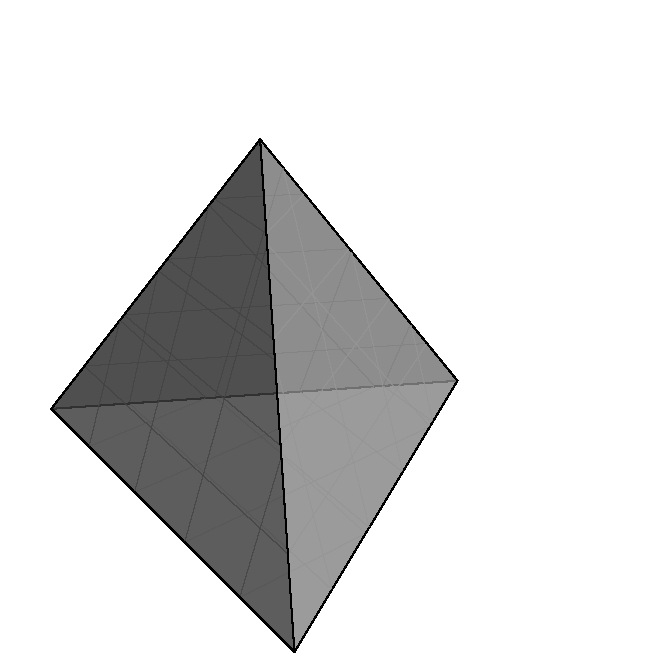
\includegraphics[scale=.5]{../graphics/pyr.pdf}
\]
Since three-dimensional objects are hard to view on a flat sheet of
paper, sometimes we think about them by taking cross sections:
\[
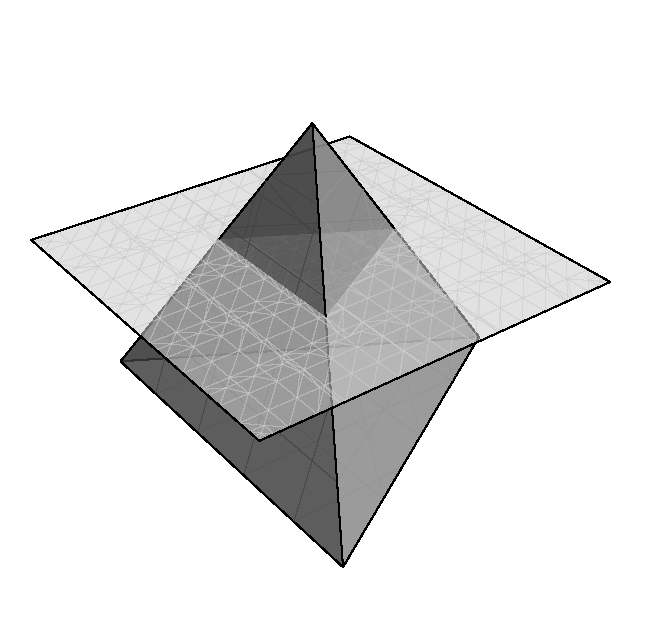
\includegraphics[scale=.5]{../graphics/planeCross.pdf}
\]
We're going to build a triangular-based pyramid out of numbers. Here
are the first four cross sections:
\[
1 \qquad 
\begin{tabular}{@{\,}c@{\,}c@{\,}c@{\,}}
1 & & 1\\
 & 1 & 
\end{tabular}
\qquad 
\begin{tabular}{@{\,}c@{\,}c@{\,}c@{\,}c@{\,}c@{\,}}
1 & & 2 & & 1 \\
 & 2 & & 2 &  \\
 & & 1 & &  
\end{tabular}
\qquad
\begin{tabular}{@{\,}c@{\,}c@{\,}c@{\,}c@{\,}c@{\,}c@{\,}c@{\,}}
1 & & 3 & & 3 & & 1 \\
 & 3 & & 6 & & 3 &  \\ 
 & & 3 & & 3 & &  \\ 
 & & & 1 & & &  
\end{tabular}
\]
This pyramid that we are building is called \textbf{Pascal's
  pyramid}.\index{Pascal's!pyramid}

\begin{prob} 
Give the next two cross sections of Pascal's pyramid. Explain your
reasoning.
\end{prob}


\begin{prob} 
Do you see any connections to Pascal's Triangle in Pascal's pyramid?
Explain what you see.
\end{prob}


\begin{prob} Use the Binomial Theorem to expand:
\[
(a + x)^3
\]
\end{prob}



\begin{prob} 
Replace $x$ above with $b+c$, and use the Binomial Theorem again along
with your computation above to expand:
\[
(a + b + c)^3
\]
\end{prob}


\begin{prob} 
What do you notice about the coefficients in the expansion of $(a + b + c)^3$?
\end{prob}


\begin{prob} Explain how the trinomial coefficient
\[
\binom{n}{j,k} = \frac{n!}{j! k!(n-j-k)!}
\]
corresponds to entries of Pascal's pyramid. Feel free to draw diagrams
and give examples.
\end{prob}

\begin{prob} 
The trinomial coefficient $\binom{n}{j,k}$ has the following
``physical'' meaning: It is the number of ways one can choose $j$
objects and $k$ objects from a set of $n$ objects. Try a couple of
relevant and revealing examples to provide evidence for this claim.
\end{prob}

\begin{prob}  
Explain how Pascal's Triangle is formed. In your explanation, use the
notation $\binom{n}{j,k}$. If you were so inclined to do so, could you
state a single equation that basically encapsulates your explanation
above?
\end{prob}


\begin{prob} 
Use Pascal's pyramid to expand:
\[
(a + b + c)^4
\]
Try to formulate a ``Trinomial Theorem.''
\end{prob}

\begin{prob} Use your Trinomial Theorem to explain why the numbers in the $n$th cross section of Pascal's pyramid sum to $3^n$.
\end{prob}

%%%%%%%%%%%%%%%%%%%%%%%%%%%%%%%%%%%%%%%%%%%%
%%%%%%%%%%%%%%%%%%%%%%%%%%%%%%%%%%%%%%%%%%%%
%% REF - R. L. Keeney and James F. Ramaley
%% Mathematics Magazine, Vol. 42, No. 4 (Sep., 1969), pp. 210-213 
%%

%\documentclass[handout]{ximera}
\documentclass{ximera}

\usepackage{gensymb}
\usepackage{tabularx}
\usepackage{mdframed}
\usepackage{pdfpages}
%\usepackage{chngcntr}

\let\problem\relax
\let\endproblem\relax

\newcommand{\property}[2]{#1#2}




\newtheoremstyle{SlantTheorem}{\topsep}{\fill}%%% space between body and thm
 {\slshape}                      %%% Thm body font
 {}                              %%% Indent amount (empty = no indent)
 {\bfseries\sffamily}            %%% Thm head font
 {}                              %%% Punctuation after thm head
 {3ex}                           %%% Space after thm head
 {\thmname{#1}\thmnumber{ #2}\thmnote{ \bfseries(#3)}} %%% Thm head spec
\theoremstyle{SlantTheorem}
\newtheorem{problem}{Problem}[]

%\counterwithin*{problem}{section}



%%%%%%%%%%%%%%%%%%%%%%%%%%%%Jenny's code%%%%%%%%%%%%%%%%%%%%

%%% Solution environment
%\newenvironment{solution}{
%\ifhandout\setbox0\vbox\bgroup\else
%\begin{trivlist}\item[\hskip \labelsep\small\itshape\bfseries Solution\hspace{2ex}]
%\par\noindent\upshape\small
%\fi}
%{\ifhandout\egroup\else
%\end{trivlist}
%\fi}
%
%
%%% instructorIntro environment
%\ifhandout
%\newenvironment{instructorIntro}[1][false]%
%{%
%\def\givenatend{\boolean{#1}}\ifthenelse{\boolean{#1}}{\begin{trivlist}\item}{\setbox0\vbox\bgroup}{}
%}
%{%
%\ifthenelse{\givenatend}{\end{trivlist}}{\egroup}{}
%}
%\else
%\newenvironment{instructorIntro}[1][false]%
%{%
%  \ifthenelse{\boolean{#1}}{\begin{trivlist}\item[\hskip \labelsep\bfseries Instructor Notes:\hspace{2ex}]}
%{\begin{trivlist}\item[\hskip \labelsep\bfseries Instructor Notes:\hspace{2ex}]}
%{}
%}
%% %% line at the bottom} 
%{\end{trivlist}\par\addvspace{.5ex}\nobreak\noindent\hung} 
%\fi
%
%


\let\instructorNotes\relax
\let\endinstructorNotes\relax
%%% instructorNotes environment
\ifhandout
\newenvironment{instructorNotes}[1][false]%
{%
\def\givenatend{\boolean{#1}}\ifthenelse{\boolean{#1}}{\begin{trivlist}\item}{\setbox0\vbox\bgroup}{}
}
{%
\ifthenelse{\givenatend}{\end{trivlist}}{\egroup}{}
}
\else
\newenvironment{instructorNotes}[1][false]%
{%
  \ifthenelse{\boolean{#1}}{\begin{trivlist}\item[\hskip \labelsep\bfseries {\Large Instructor Notes: \\} \hspace{\textwidth} ]}
{\begin{trivlist}\item[\hskip \labelsep\bfseries {\Large Instructor Notes: \\} \hspace{\textwidth} ]}
{}
}
{\end{trivlist}}
\fi


%% Suggested Timing
\newcommand{\timing}[1]{{\bf Suggested Timing: \hspace{2ex}} #1}




\hypersetup{
    colorlinks=true,       % false: boxed links; true: colored links
    linkcolor=blue,          % color of internal links (change box color with linkbordercolor)
    citecolor=green,        % color of links to bibliography
    filecolor=magenta,      % color of file links
    urlcolor=cyan           % color of external links
}

\title{You Can Count on It!}
\author{Bart Snapp and Brad Findell}

\outcome{Learning outcome goes here.}

\begin{document}
\begin{abstract}
Abstract goes here.  
\end{abstract}
\maketitle

\label{A:countOnIt}
\begin{teachingnote}
 The words permutation and combination tend to promote formulaic thinking rather than careful reasoning.  And students tend to ask ``Does order matter?'' in ways that don't help them with the reasoning. 

The major purposes of this activity: (1) the multiplication principle of counting, supported by a drawn or imagined tree diagram; and (2) strong explanatory thinking around ``$n$ choose $k$,'' connecting to both traffic lights and Pascal's triangle.  

Although students will find formulas for ``$n$ choose $k$'' to be useful, we need not emphasize formulas for permutations because the multiplication principle provides it for free.   (See also the final exam review document from 2014.)
\end{teachingnote}

\begin{problem}
The Diet-Lite restaurant offers 3 entr\'ees, 4 side dishes, 2 desserts
and 5 kinds of drinks.  
\begin{enumerate}
\item If you were going to select a dinner with one
entr\'ee and one side dish, how many different dinners could you order?  Explain your reasoning.  
\item If you were going to select a dinner with one
entr\'ee, one side dish, one dessert, and one drink, how many different
dinners could you order?
\end{enumerate}
\end{problem}

\begin{problem}
Suppose an Ohio license plate consists of two letters followed by two
digits followed by two letters.  How many different
license plates can be made if: 
\begin{enumerate}
\item There are no more restrictions on the
numbers or letters.
\item  There are no repeats of numbers or letters.
\end{enumerate}
\end{problem}

\begin{problem}
Naming officers and choosing a committee.
\begin{enumerate}
\item How many ways can a chairperson, secretary, and treasurer be named in a club of 10 people?  
\item How many ways can a committee of 3 people be chosen from this same club?
\item Explain using how the answer to (b) makes sense by beginning with the answer to (a) and then ``adjusting'' for overcounting.  
\item Generalize part (c) to explain a formula for the number of ways that a committee of $k$ people can be chosen from a club of $n$ members, where $k$ and $n$ are counting numbers with $k<n$.
\end{enumerate}
\end{problem}

\begin{teachingnote}
The following problems are optional.
\end{teachingnote}

\begin{problem}
Six coins are flipped separately (e.g., HTHHHT is different from THHHTH).  How many different results are
possible?
\end{problem}

\begin{problem}
A pizza shop always puts cheese on their pizzas.  If the shop offers
$n$ additional toppings, how many different pizzas can be ordered?
(Note: A plain cheese pizza is an option.)
\end{problem}


%\begin{problem}
%The Pig-Out restaurant offers 5 entrees, 8 side dishes, 12 desserts,
%and 6 kinds of drinks.  If you were going to select a dinner with 3
%entr\'ees, 4 side dishes, 7 desserts, and one drink, how many
%different dinners could you order?
%\end{problem}

\end{document}


\newpage
\section{Which Road Should We Take?}

\begin{prob} Consider a six-sided die. Without actually rolling a die, guess the number of 1's, 2's, 3's, 4's, 5's, and 6's you would obtain in 50 rolls. Record your predictions in the chart below:
\begin{center}\textbf{Predictions}\end{center}
\[
\begin{tabular}{|c|c|c|c|c|c|c|}\hline
\# of 1's & \# of 2's & \# of 3's & \# of 4's & \# of 5's & \# of 6's & Total \\ \hline 
\rule[0mm]{0mm}{7mm} \hspace{15mm} &  \hspace{15mm} & \hspace{15mm} & \hspace{15mm} & \hspace{15mm} & \hspace{15mm} & \hspace{15mm}\\ \hline
\end{tabular}
\]


Now roll a die 50 times and record the number of 1's, 2's, 3's, 4's, 5's, and 6's you obtain.  
\begin{center}\textbf{Experimental Results}\end{center}
\[
\begin{tabular}{|c|c|c|c|c|c|c|}\hline
\# of 1's & \# of 2's & \# of 3's & \# of 4's & \# of 5's & \# of 6's & Total \\ \hline 
\rule[0mm]{0mm}{7mm} \hspace{15mm} &  \hspace{15mm} & \hspace{15mm} & \hspace{15mm} & \hspace{15mm} & \hspace{15mm} & \hspace{15mm}\\ \hline
\end{tabular}
\]
How did you come up with your predictions? How do your predictions
compare with your actual results? Now make a chart to combine your
data with that of the rest of the class.

\end{prob}

\paragraph{Experiment 1}  We investigated the results of throwing 
one die and recording what we saw (a $1$, a $2$, ..., or a $6$).  
We said that the probability of an event (for example, getting a ``3'' 
in this experiment) predicts the frequency with which we expect to see 
that event occur in a large number of trials.
You argued the $P(\text{seeing }3)=1/6$ (meaning we
expect to get a $3$ in about $1/6$ of our trials) because there were
six different outcomes, only one of them is a $3$, and you expected
each outcome to occur about the same number of times.

\paragraph{Experiment 2}
We are now investigating the results of throwing two dice and
recording the sum of the faces. We are trying to analyze the
probabilities associated with these sums.  Let's focus first on
$P(sum=2)=?$. We might have some different theories, such 
as the following:


\paragraph{Theory 1} 
$P(\text{sum}=2)=1/11$. 

It is proposed that a sum of $2$ was $1$ out
of the $11$ possible sums $\{2,3,4,5,6,7,8,9,10,11,12\}$.


\paragraph{Theory 2} 
$P(\text{sum}=2)=1/21$. 

It is proposed that a sum of $2$ was $1$ of
$21$ possible results, counting $1+3$ as the same as $3+1$:

\[
\begin{array}{cccccc}
1+1 & - & - & - & - & - \\
2+1 & 2+2 & - & - & - & - \\
3+1 & 3+2 & 3+3 & - & - & - \\
4+1 & 4+2 & 4+3 & 4+4 & - & - \\
5+1 & 5+2 & 5+3 & 5+4 & 5+5 & - \\
6+1 & 6+2 & 6+3 & 6+4 & 6+5 & 6+6 
\end{array}
\]

\begin{teachingnote}
Some might suggest that the sample space is better thought of as ordered pairs rather than sums.  In any case, the upshot is that for anything we do with the two dice, the sample space has 36 elements.  Then the following activity, Lumpy and Eddy, might be redundant.
\end{teachingnote}

\begin{prob}
Propose your own Theory 3.  
\end{prob}

%\subparagraph{Theory 3} $P(\text{sum}=2)=1/36$. 
%
%It was proposed that a
%sum of $2$ was $1$ of $36$ possible results, counting $1+3$ as
%different from $3+1$:
%\[
%\begin{array}{cccccc}
%1+1 & 1+2 & 1+3 & 1+4 & 1+5 & 1+6 \\
%2+1 & 2+2 & 2+3 & 2+4 & 2+5 & 2+6 \\
%3+1 & 3+2 & 3+3 & 3+4 & 3+5 & 3+6 \\
%4+1 & 4+2 & 4+3 & 4+4 & 4+5 & 4+6 \\
%5+1 & 5+2 & 5+3 & 5+4 & 5+5 & 5+6 \\
%6+1 & 6+2 & 6+3 & 6+4 & 6+5 & 6+6 
%\end{array}
%\]

\begin{prob}
Test all theories by computing $P(2)$, $P(3)$, \dots , $P(12)$ for each theory and comparing to the dice rolls recorded by the class.  What do you notice?  
\end{prob}

\begin{prob}
Which theory do you like best?  Why?
\end{prob}


\begin{prob}
 How could we test our theory further?
\end{prob}

%\documentclass[handout]{ximera}
\documentclass{ximera}

\usepackage{gensymb}
\usepackage{tabularx}
\usepackage{mdframed}
\usepackage{pdfpages}
%\usepackage{chngcntr}

\let\problem\relax
\let\endproblem\relax

\newcommand{\property}[2]{#1#2}




\newtheoremstyle{SlantTheorem}{\topsep}{\fill}%%% space between body and thm
 {\slshape}                      %%% Thm body font
 {}                              %%% Indent amount (empty = no indent)
 {\bfseries\sffamily}            %%% Thm head font
 {}                              %%% Punctuation after thm head
 {3ex}                           %%% Space after thm head
 {\thmname{#1}\thmnumber{ #2}\thmnote{ \bfseries(#3)}} %%% Thm head spec
\theoremstyle{SlantTheorem}
\newtheorem{problem}{Problem}[]

%\counterwithin*{problem}{section}



%%%%%%%%%%%%%%%%%%%%%%%%%%%%Jenny's code%%%%%%%%%%%%%%%%%%%%

%%% Solution environment
%\newenvironment{solution}{
%\ifhandout\setbox0\vbox\bgroup\else
%\begin{trivlist}\item[\hskip \labelsep\small\itshape\bfseries Solution\hspace{2ex}]
%\par\noindent\upshape\small
%\fi}
%{\ifhandout\egroup\else
%\end{trivlist}
%\fi}
%
%
%%% instructorIntro environment
%\ifhandout
%\newenvironment{instructorIntro}[1][false]%
%{%
%\def\givenatend{\boolean{#1}}\ifthenelse{\boolean{#1}}{\begin{trivlist}\item}{\setbox0\vbox\bgroup}{}
%}
%{%
%\ifthenelse{\givenatend}{\end{trivlist}}{\egroup}{}
%}
%\else
%\newenvironment{instructorIntro}[1][false]%
%{%
%  \ifthenelse{\boolean{#1}}{\begin{trivlist}\item[\hskip \labelsep\bfseries Instructor Notes:\hspace{2ex}]}
%{\begin{trivlist}\item[\hskip \labelsep\bfseries Instructor Notes:\hspace{2ex}]}
%{}
%}
%% %% line at the bottom} 
%{\end{trivlist}\par\addvspace{.5ex}\nobreak\noindent\hung} 
%\fi
%
%


\let\instructorNotes\relax
\let\endinstructorNotes\relax
%%% instructorNotes environment
\ifhandout
\newenvironment{instructorNotes}[1][false]%
{%
\def\givenatend{\boolean{#1}}\ifthenelse{\boolean{#1}}{\begin{trivlist}\item}{\setbox0\vbox\bgroup}{}
}
{%
\ifthenelse{\givenatend}{\end{trivlist}}{\egroup}{}
}
\else
\newenvironment{instructorNotes}[1][false]%
{%
  \ifthenelse{\boolean{#1}}{\begin{trivlist}\item[\hskip \labelsep\bfseries {\Large Instructor Notes: \\} \hspace{\textwidth} ]}
{\begin{trivlist}\item[\hskip \labelsep\bfseries {\Large Instructor Notes: \\} \hspace{\textwidth} ]}
{}
}
{\end{trivlist}}
\fi


%% Suggested Timing
\newcommand{\timing}[1]{{\bf Suggested Timing: \hspace{2ex}} #1}




\hypersetup{
    colorlinks=true,       % false: boxed links; true: colored links
    linkcolor=blue,          % color of internal links (change box color with linkbordercolor)
    citecolor=green,        % color of links to bibliography
    filecolor=magenta,      % color of file links
    urlcolor=cyan           % color of external links
}

\title{Lumpy and Eddie}
\author{Bart Snapp and Brad Findell}

\outcome{Learning outcome goes here.}

\begin{document}
\begin{abstract}
Abstract goes here.  
\end{abstract}
\maketitle

Two ancient philosophers, Lumpy and Eddie, were sitting on rocks
flipping coins. 

\begin{problem} Lumpy and Eddie wondered about the probability of obtaining both a head and a tail. Here is how it went:
\begin{quote}
Eddie argued the following: ``Look Lumpy, it's clear to me that when
we flip two coins, we should get one of each about half the time
because there are two possibilities: They're either the same or
different.'' Lumpy, on the other hand, argued this way: ``Eddie, stop
being a wise guy! If we flipped two coins, we should expect both a
head and tail to come up about a third of the time because there are
only three possibilities: two heads, two tails, and one of each.''
\end{quote}
Which, if any, of these two guys is right?  Is there another answer?
\end{problem}

\begin{problem}
Next Lumpy and Eddie threw a third coin in the mix and wondered about
the probability of obtaining 2 heads and a tail or 2 tails and a head.
\begin{enumerate}
\item What would Lumpy say in this case?
\item What would Eddie say in this case?
\end{enumerate}
Be sure to clearly explain why you think they would answer in the way
you suggest.
\end{problem}

\end{document}


\newpage
\section{Go Climb a Tree!} 

%\fixnote{Make this more careful and focused.  Perhaps begin with one and one freethrows in basketball as a reason to draw a tree diagram.  In all problems, we need to assume independence.  In problem 3, best of five games would be enoug.  In problem 5, we mean by guessing.}

In this activity, we'll evaluate the probabilities of complex events
using tree diagrams, fraction arithmetic, and counting.

% Removed the following problem because the multiplication connection is not fully made.  Restore if we can find a way. 
%
%\begin{prob}
%Give a story problem that is modeled by the expression:
%\[
%\frac{3}{7} \times \frac{2}{5}
%\]  
%Let the start of the story be: ``$2/5$ of the class are girls.''  Once
%you have the story, solve it using pictures (use rectangles for the
%wholes) and explain why it makes sense that multiplying fractions is
%the same as multiplying the numerators and multiplying the
%denominators.
%\end{prob}
%
%Removed the following problem because weather events are not independent.  
%\begin{prob}
%The Weather Channel has predicted that there is a 70\% chance of rain today, a 20\% chance of rain tomorrow, and a 40\% chance of rain the day after tomorrow.  Use a tree diagram to help answer the following:
%\begin{enumerate}
%\item What is the probability that it will rain today and not rain tomorrow? 
%\item What is the probability it will rain on exactly one of the first two days?
%\item What is the probability that it will rain today, not rain tomorrow, and rain the following day?
%\item What is the probability that it will rain on exactly two of the three days?
%\item What is the probability it will rain on all three days?
%\item What is the probability it won't rain at all?
%\item What is the probability it will rain on at least one of the days?
%\end{enumerate}
%\end{prob}

\begin{prob}
Place \textbf{three green} cubes and \textbf{three red} cubes in a bag.  Without looking, draw three cubes, one at a time, \textbf{without replacement}.  
\begin{enumerate}
\item Write probabilities in the tree diagram below to organize the possible outcomes and compute their probabilities.  
\[
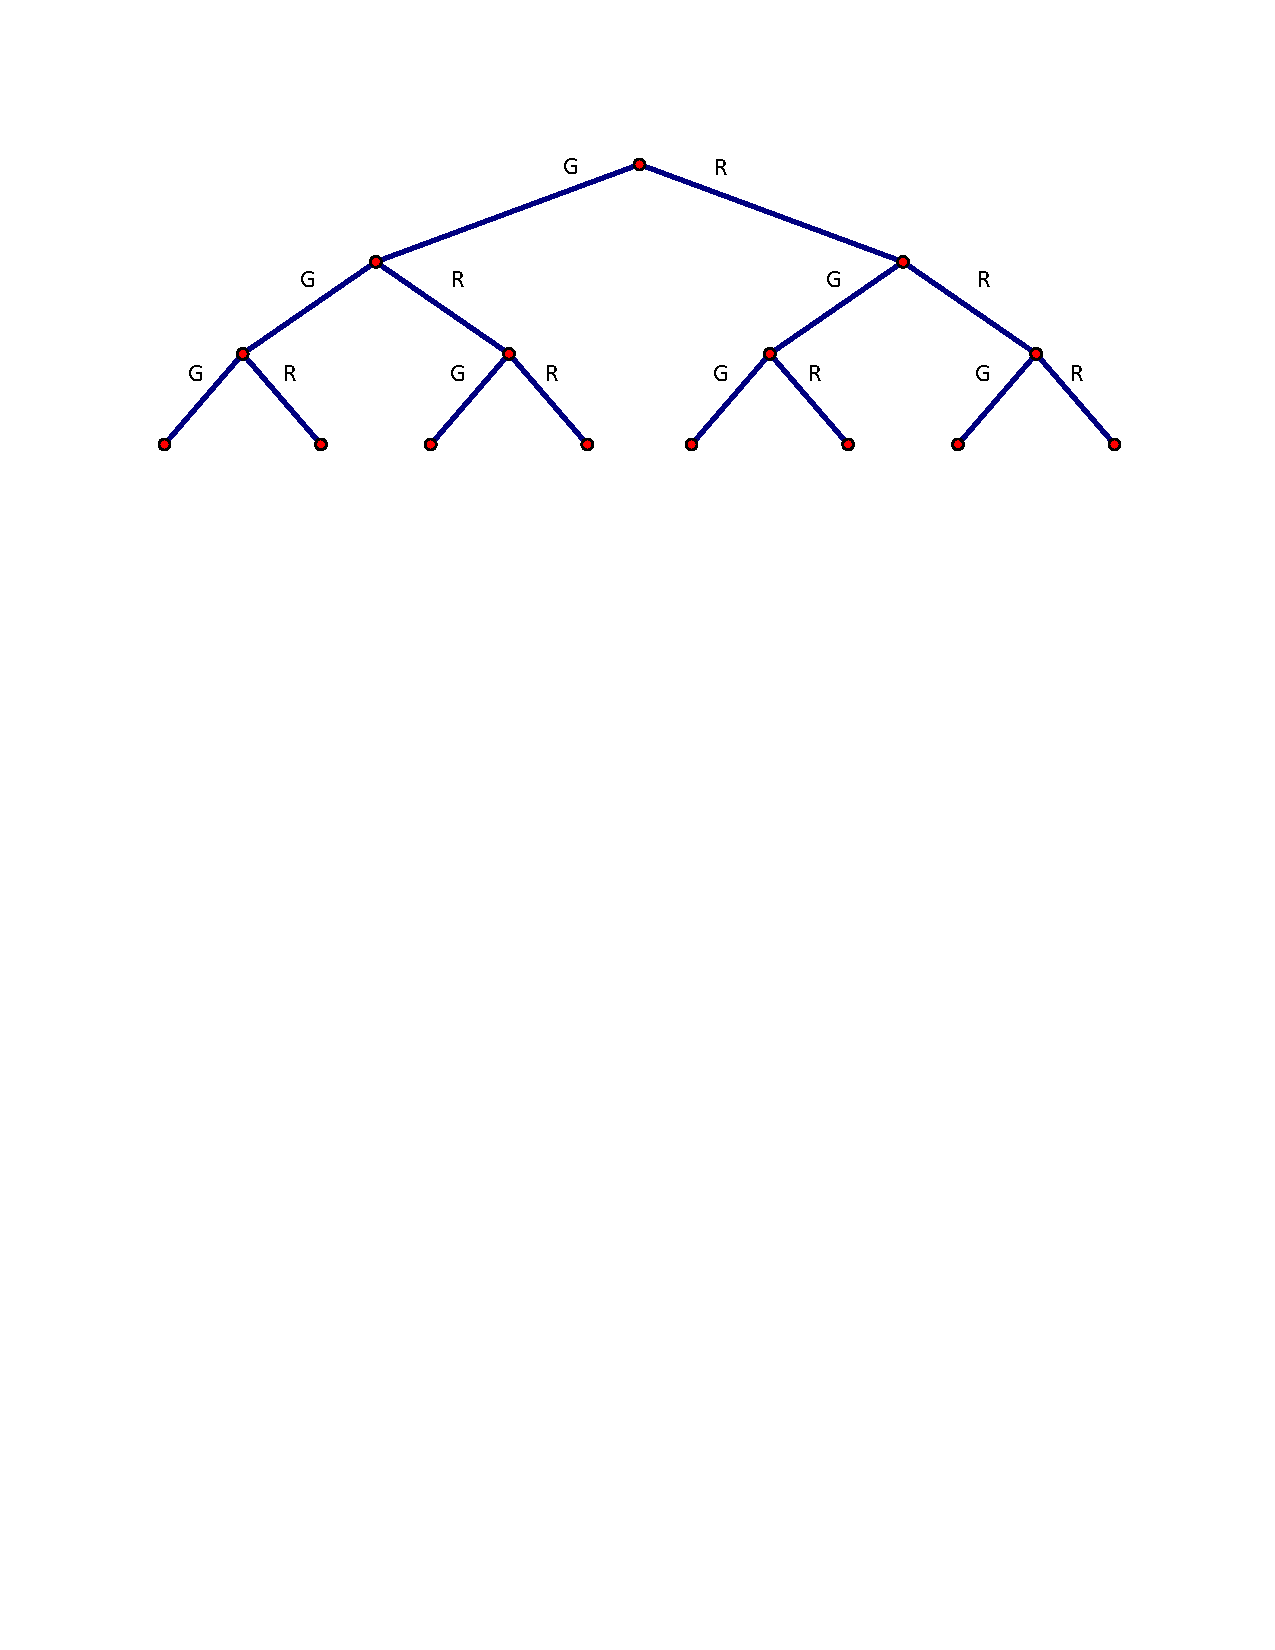
\includegraphics[scale=0.8]{../graphics/tree.pdf}
\]
\vspace{.15in}
\item What is the probability of three reds? 
\item What is the probability of two reds and a green? 
\item What is the probability of one red and two greens? 
\item What is the probability of three greens? 
\item If the first cube is green, what is the probability that the second cube is red? 
\item If the first cube is red, what is the probability that the second cube is red? 
\item What is the probability that the second cube is red?  
\end{enumerate}
\end{prob}

\newpage
\begin{prob}
Place \textbf{three green} cubes and \textbf{three red cubes} in a bag.  Without looking, draw three cubes, one at a time, \textbf{this time with replacement}.  
\begin{enumerate}
\item Write probabilities in the tree diagram below to organize the possible outcomes and compute their probabilities.  
\[
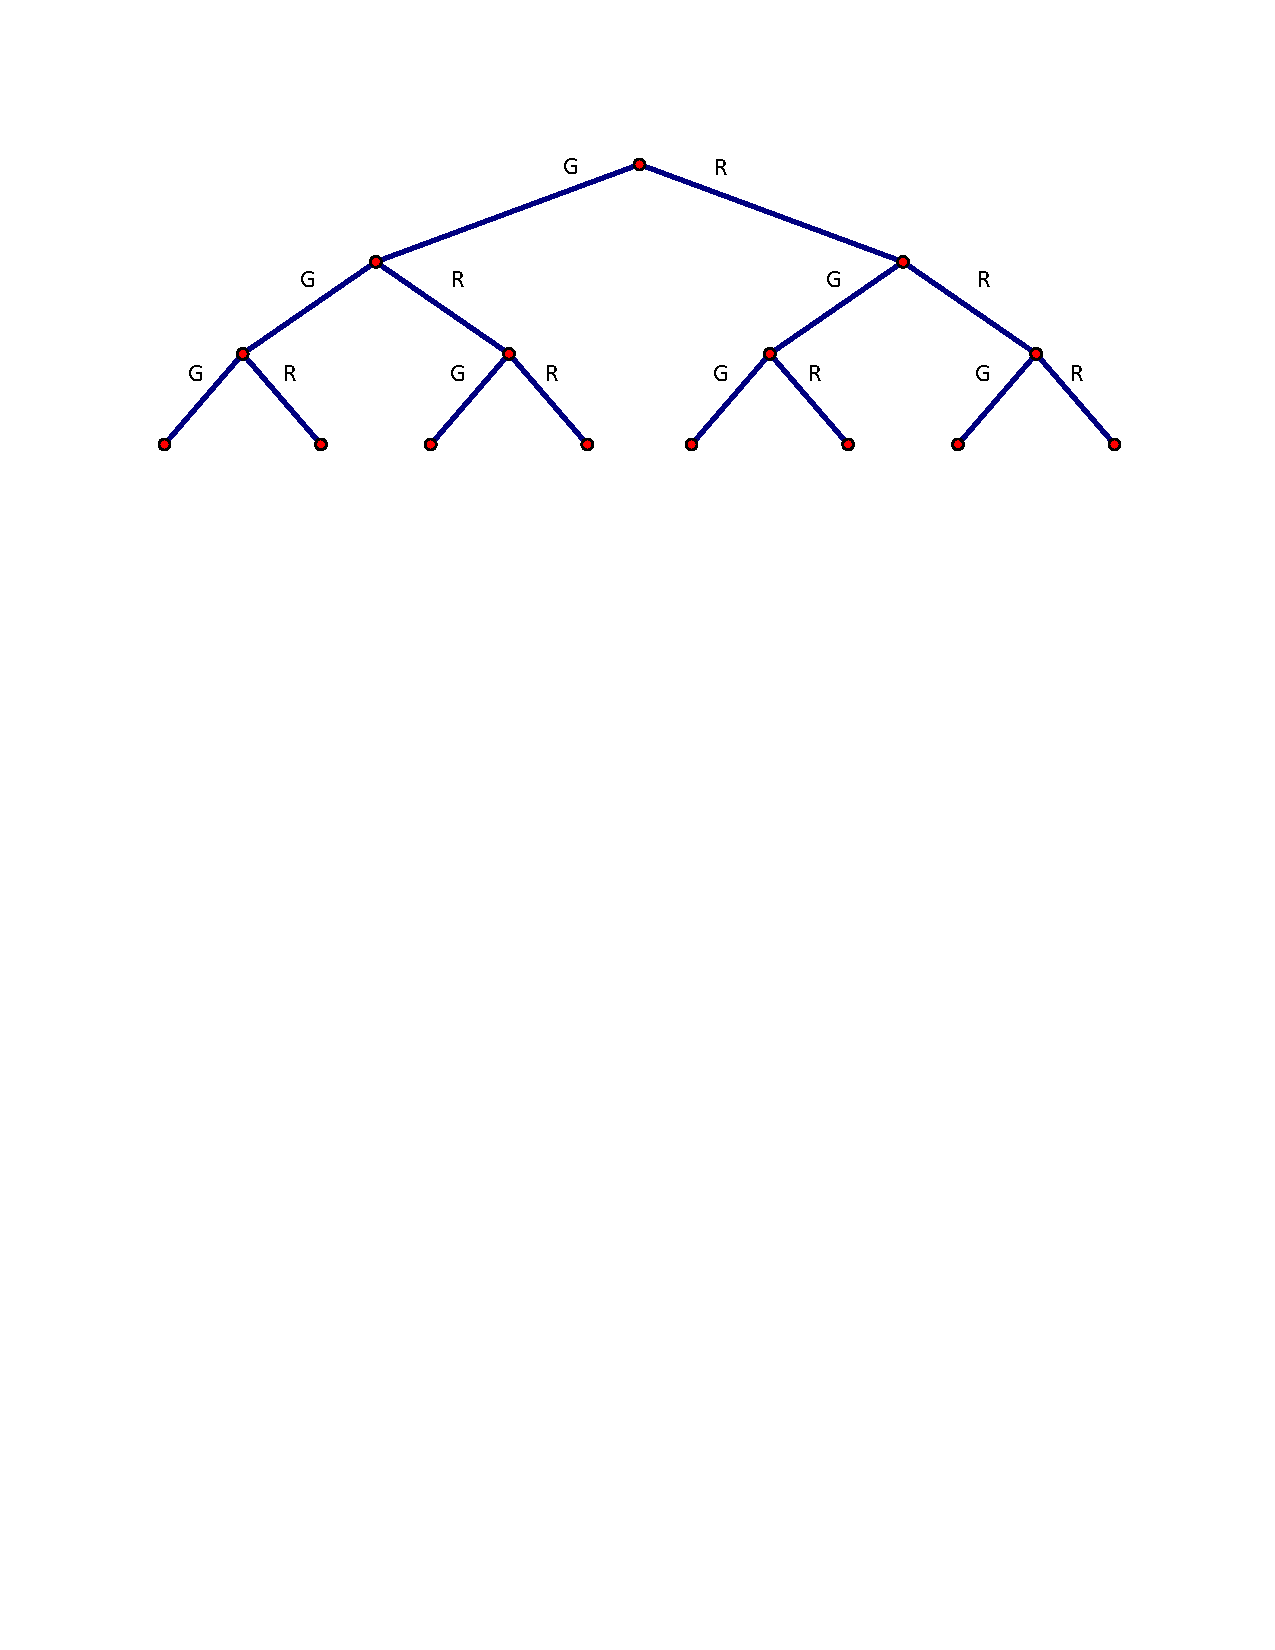
\includegraphics[scale=0.8]{../graphics/tree.pdf}
\]
\vspace{.15in}
\item What is the probability of three reds? 
\item What is the probability of two reds and a green? 
\item What is the probability of one red and two greens? 
\item What is the probability of three greens? 
\item If the first cube is green, what is the probability that the second cube is red? 
\item If the first cube is red, what is the probability that the second cube is red? 
\item What is the probability that the second cube is red?  
\item Use the words "dependent" and "independent" to contrast the probability that the second cube is red in this and the previous scenario.  
\end{enumerate}
\end{prob}

\newpage
\begin{prob}
This time, place \textbf{two green} cubes and \textbf{three red} cubes in a bag.  Without looking, draw three cubes, one at a time, \textbf{again with replacement}.  
\begin{enumerate}
\item Write probabilities in the tree diagram below to organize the possible outcomes and compute their probabilities.  
\[
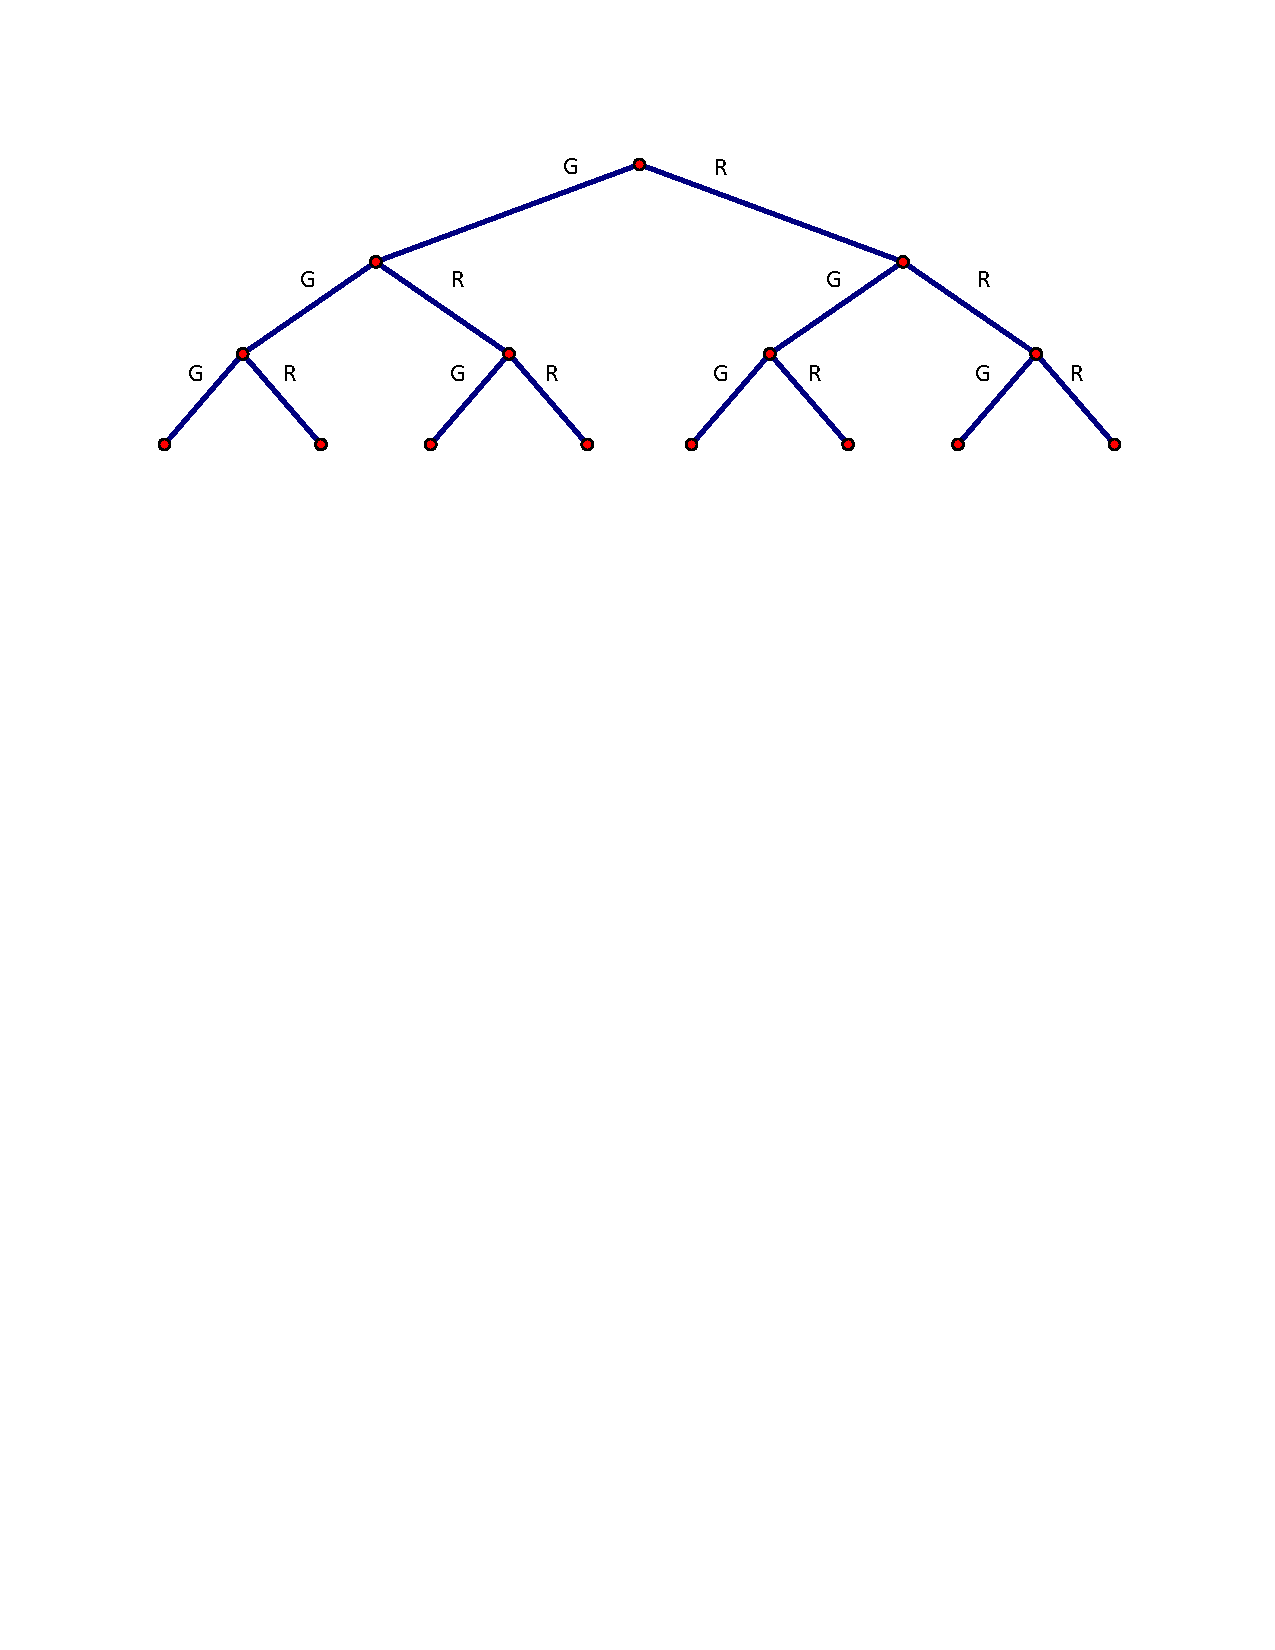
\includegraphics[scale=0.8]{../graphics/tree.pdf}
\]
\vspace{.15in}
\item What is the probability of three reds? 
\item What is the probability of two reds and a green? 
\item What is the probability of one red and two greens? 
\item What is the probability of three greens? 
\item If the first cube is green, what is the probability that the second cube is red? 
\item If the first cube is red, what is the probability that the second cube is red? 
\item What is the probability that the second cube is red?  
\item Is the probability that the second cube is red independent of the outcome of the first cube?  Explain. 
\item In the previous scenario, some outcomes are equally likely.  Is that true here?  Why or why not? 
\end{enumerate}
\end{prob}

\newpage

\begin{prob}
Suppose the Indians and the Yankees are to face each other in a best-of-three series.  Suppose the probability that the Indians will win any game is 60\%, and suppose the outcomes of the games are independent of one another.  
\begin{enumerate}
\item Draw a tree diagram for the series.  
\item What is the probability that the Indians win games 1 and 3 to win the series?
\item What is the probability that the Indians win the series in exactly 3 games?
\item What is the probability that the Indians win the series?
\end{enumerate}
\end{prob}


\begin{prob} 
Fred the Slob has an unreliable car that starts only 60\% of the days.
If the car doesn't start, poor Fred must walk the one block to work.
This week, he is slated to work 5 days (Monday through Friday).  
\begin{enumerate}
\item What is the probability that Fred will walk on Monday and Wednesday
and drive the other days?
\item What is the probability that Fred will drive on exactly 4 of the days? 
\item What is the probability that poor Fred will have to walk on at least two of the days?
\end{enumerate}
\end{prob}






%\begin{prob}
%Use the techniques of this activity (i.e., using a special case and
%fraction arithmetic to help investigate a more general case) to find
%the probability of passing a 10-question true/false test by guessing if you
%must get 70\% or more correct to pass.
%\end{prob}

\newpage
\section{They'll Fall for Anything!}\label{A:fallForAnything}

What is incorrect about the following reasoning? Be specific!

\begin{prob}
Herman says that if you pick a United States citizen at random, the
probability of selecting a citizen from Indiana is because Indiana is
one of 50 equally likely states to be selected.
\end{prob}


\begin{prob}
Jerry has set up a game in which one wins a prize if he/she selects an
orange chip from a bag.  There are two bags to choose from.  One has 2
orange and 4 green chips.  The other bag has 7 orange and 7 green
chips.  Jerry argues that you have a better chance of winning by
drawing from the second bag because there are more orange chips in it.
\end{prob}

\begin{prob}
Gil the Gambler says that it is just as likely to flip 5 coins and get
exactly 3 heads as it is to flip 10 coins and get exactly 6 heads
because
\[
\frac{3}{5} = \frac{6}{10}
\]
\end{prob}

\begin{prob}
We draw 4 cards without replacement from a deck of 52.  Know-it-all
Ned says the probability of obtaining all four 7's is
$\frac{4}{\binom{52}{4}}$ because there are ways to select the
$\binom{52}{4}$ 4 cards and there are four 7's in the deck.
\end{prob} 

\begin{prob}
At a festival, Stealin' Stan gives Crazy Chris the choice of one of
three prizes---each of which was hidden behind a door.  One of the
doors has a fabulous prize behind it while the other two doors each
have a ``zonk'' (a free used tube of toothpaste, etc.).  Crazy Chris
chooses Door \#1.  Before opening that door, Stealin' Stan shows Chris
that hidden behind Door \#3 is a zonk and gives Chris the option to
keep Door \#1 or switch to Door \#2.  Chris says, ``Big deal.  It doesn't
help my chances of winning to switch or not switch.''
\end{prob}

%\newpage
\activity\section{The Harmonic Triangle}\index{harmonic triangle} 

Leibniz, one of the inventors of calculus, dreamed up this beast while
trying to solve a problem posed to him by Huygens:
\[
\begin{tabular}{@{\,}c@{\,}c@{\,}c@{\,}c@{\,}c@{\,}c@{\,}c@{\,}c@{\,}c@{\,}}
& & & & $\frac{1}{1}$ & & & & \\
& & & $\frac{1}{2}$ & & $\frac{1}{2}$ & & & \\
& & $\frac{1}{3}$ & & $\frac{1}{6}$ & & $\frac{1}{3}$ & & \\
& $\frac{1}{4}$ & & $\frac{1}{12}$ & & $\frac{1}{12}$ & & $\frac{1}{4}$ &\\
$\frac{1}{5}$ & & $\frac{1}{20}$ & & $\frac{1}{30}$ & & $\frac{1}{20}$ & & $\frac{1}{5}$
\end{tabular}
\]

\begin{prob} 
What relationships can you find between the entries of the triangle as
we move from row to row?
\end{prob}


\begin{prob} What are the next two rows? Clearly articulate how to produce more rows of the Harmonic Triangle.
\end{prob}

\begin{prob} Explain how the following expression
\[
\frac{1}{k\binom{n}{k}}
\]
corresponds to entries of the Harmonic Triangle. Feel free to draw
diagrams and give examples.
\end{prob}

\begin{prob}  
Explain how the Harmonic Triangle is formed. In your explanation, use
the notation
\[
\frac{1}{k\binom{n}{k}}
\]
If you were so inclined to do so, could you state a single equation
that basically encapsulates your explanation above?
\end{prob}

\begin{prob} 
Can you explain why the numerators of the fractions in the Harmonic
Triangle must always be $1$?
\end{prob}


\begin{prob} Explain how to use the Harmonic Triangle to go from:
\[
\frac{1}{2} + \frac{1}{6} + \frac{1}{12} + \frac{1}{20}+\cdots
\]
to
\[
\left(1 - \frac{1}{2}\right) + \left(\frac{1}{2}-\frac{1}{3}\right) + 
\left(\frac{1}{3}- \frac{1}{4}\right) + \left(\frac{1}{4}-\frac{1}{5}\right) + \cdots 
\]
Conclude by explaining why Leibniz said:
\[
\frac{1}{2} + \frac{1}{6} + \frac{1}{12} + \frac{1}{20}+\cdots = 1
\]
\end{prob}

\begin{prob} Explain how to use the Harmonic Triangle to go from:
\[
\frac{1}{3} + \frac{1}{12} + \frac{1}{30} + \frac{1}{60}+\cdots 
\]
to
\[
\left(\frac{1}{2} - \frac{1}{6}\right) + \left(\frac{1}{6}-\frac{1}{12}\right) + 
\left(\frac{1}{12}- \frac{1}{20}\right) + \left(\frac{1}{20}-\frac{1}{30}\right) + \cdots 
\]
Conclude by explaining why Leibniz said:
\[
\frac{1}{3} + \frac{1}{12} + \frac{1}{30} + \frac{1}{60}+\cdots = \frac{1}{2}
\]
\end{prob}

\begin{prob} 
Can you generalize the results above? Can you give a list of infinite
sums and conjecture what they will converge to?
\end{prob}





%%%%%%%%%%%%%%%%%%%%%%%%%%%%%%%%%%%%%%%%%%%%
%%%%%%%%%%%%%%%%%%%%%%%%%%%%%%%%%%%%%%%%%%%%
%% REF - Cut the knot
%% http://www.cut-the-knot.org/Curriculum/Combinatorics/LeibnitzTriangle.shtml
%% The Origins of the Infinitesimal Calculus. Margaret E. Baron. Dover 1969  
%%

%\newpage
\activity\section{Whoops!}


Niccol\`{o} Fontana Tartaglia was a great mathematician of the
1500's. Once he claimed claimed that the sums
\[
1+2+4, \qquad 1+2+4+8, \qquad 1+2+4+8+16, \qquad\text{and so on,} 
\]
are alternately prime and composite.

\begin{prob}
Investigate Tartaglia's claim and report your findings.
\end{prob}

One thing that would make analyzing this claim easier would be if we
had a simple formula for his sums. 

\begin{prob} 
Using a table, see if you can guess a formula for Tartaglia's sums.
\end{prob}

\begin{prob} 
Can you explain why your formula holds? Can you generalize your
formula?
\end{prob}


\begin{prob}
Expand out the following:
\begin{enumerate}
\item $(a^2 -1)(1 + a^2 + a^{2 \cdot 2})$
\item $(a^2 -1)(1 + a^2 + a^{2 \cdot 2}+a^{3 \cdot 2})$  
\item $(a^2 -1)(1 + a^2 + a^{2 \cdot 2}+a^{3 \cdot 2} + a^{4 \cdot 2})$ 
\end{enumerate}
\end{prob}

\begin{prob} Expand out the following:
\[
(2^a - 1)(1 + 2^a + 2^{2a} + 2^{3a} + \dots + 2^{(b-1)a})
\]
what does this say about Tartaglia's conjecture above?
\end{prob}



%\newpage
\activity\section{Big Primes}


All over the world, computers are churning away, trying to to find the
next prime. This is what is known as the Great Internet Mersenne Prime
Search---or (don't laugh) \index{GIMPS}GIMPS. If you are willing, you
too can play along and donate time on your computer. Every year or so
a new prime is found, and glory-everlasting\footnote{This might be a
slight exaggeration.} goes to the person who finds it! I will not
attempt to be up to date. Please use some inter-web-search-doo-hicky
or whatever to find the largest known prime. Please write the actual
number below:

\vspace{1in}

There is little doubt in my mind that this largest known prime will be
of the form:
\[
M_n = 2^n -1
\]
where $n$ is some number. Numbers of this form are
called \textit{Mersenne} numbers.\index{Mersenne numbers}

\begin{prob} 
Make a table of the Mersenne numbers $M_n$ for $n$ from $1$ to $10$. 
\end{prob}

\begin{prob} 
Which of the numbers in your table are prime? Make a conjecture.
\end{prob}

\begin{prob} 
Continue your table out to $M_{14}$. Check your conjecture up to this
point.
\end{prob}


\begin{prob} 
Compare this activity to the activity \textit{Whoops!} What do you
notice?
\end{prob}


By the way, we should add---$M_{n}$ grows very fast as $n$
grows. Let's do some comparisons:

\begin{prob} 
Which is bigger, the largest known Mersenne prime or the number of atoms
in \textit{you}?
\end{prob}

\begin{prob} 
Which is bigger, the largest known Mersenne prime or the number of
atoms in the planet Earth?
\end{prob}

\begin{prob} 
Which is bigger, the largest known Mersenne prime or the number of
atoms in the Sun?
\end{prob}

\begin{prob} 
Which is bigger, the largest known Mersenne prime or the number of
atoms in the visible Universe?
\end{prob}



%% \chapter{Enrichment Topics}
%% \input{../chapters/enrichment/continuedFractions.tex}
%% \input{../chapters/enrichment/music.tex}



%%%% Index and References
\input{../chapters/back}
%%%%

\begin{teachingnote}
Activities to be added or revised:  
\begin{itemize}
\item Beckmann 1G
\item Product Puzzle from Connected Mathematics Project 
\item A.13. There are many factors to consider.  Needs revision. 
\item A.20. Picture Yourself Dividing.  Include $1\frac{3}{4}\div \frac{1}{2}$. 
\item A.26. Poor Old Horatio.  Need new ratio table problems.
\item A.54  Second Differences.  Current version won't compile within notes.  
\end{itemize}
\end{teachingnote}

% Fixnote summary and other needs
%
% Highlight Deep Insights, such as
%  * The point-slope form of a line turns a non-proportional situation into a proportional one. 
%  * The sequence of partial sums of an arithmetic series is a quadratic function. 
%  * With common denominators, division of fractions ? 
%
% Fix the footnotes
%
%More problems needed: 
% 1.1. Other bases
% 1.2. Doubling and halving algorithm for multiplication 
%         Mysterious base two game
% 2.1. Models of integer arithmetic
% 3.1. Easy problems on ratio and proportional reasoning
% 	Ratio tables, going through 1, tables that aren?t ratio tables
% 3.2. More problem on quadratics, exponentials?  (Some in LaTeX comments.)
%
% Discussion:  Meaning of the equals sign somewhere
%

